% Options for packages loaded elsewhere
\PassOptionsToPackage{unicode}{hyperref}
\PassOptionsToPackage{hyphens}{url}
%
\documentclass[oneside]{article}
\usepackage{listings}
\lstdefinelanguage{es3}{
	literate=%
	{0}{{{\color{black}0}}}1
	{1}{{{\color{black}1}}}1
	{2}{{{\color{black}2}}}1
	{3}{{{\color{black}3}}}1
	{4}{{{\color{black}4}}}1
	{5}{{{\color{black}5}}}1
	{6}{{{\color{black}6}}}1
	{7}{{{\color{black}7}}}1
	{8}{{{\color{black}8}}}1
	{9}{{{\color{black}9}}}1,
	sensitive = false,
	breaklines=true,
	columns=fixed,
}
% Set Language
\lstset{
	language={es3},
	basicstyle=\small\ttfamily, % Global Code Style
	extendedchars=true, % Allows 256 instead of 128 ASCII characters
	tabsize=2, % number of spaces indented when discovering a tab 
	columns=fixed, % make all characters equal width
	keepspaces=true, % does not ignore spaces to fit width, convert tabs to spaces
	showstringspaces=false, % lets spaces in strings appear as real spaces
	breaklines=true, % wrap lines if they don't fit
	frame=trbl, % draw a frame at the top, right, left and bottom of the listing
}
\usepackage{amsmath,amssymb}
\usepackage{lmodern}
\usepackage{iftex}
\ifPDFTeX
  \usepackage[T1]{fontenc}
  \usepackage[utf8]{inputenc}
  \usepackage{textcomp} % provide euro and other symbols
\else % if luatex or xetex
  \usepackage{unicode-math}
  \defaultfontfeatures{Scale=MatchLowercase}
  \defaultfontfeatures[\rmfamily]{Ligatures=TeX,Scale=1}
\fi
% Use upquote if available, for straight quotes in verbatim environments
\IfFileExists{upquote.sty}{\usepackage{upquote}}{}
\IfFileExists{microtype.sty}{% use microtype if available
  \usepackage[]{microtype}
  \UseMicrotypeSet[protrusion]{basicmath} % disable protrusion for tt fonts
}{}
\makeatletter
\@ifundefined{KOMAClassName}{% if non-KOMA class
  \IfFileExists{parskip.sty}{%
    \usepackage{parskip}
  }{% else
    \setlength{\parindent}{0pt}
    \setlength{\parskip}{6pt plus 2pt minus 1pt}}
}{% if KOMA class
  \KOMAoptions{parskip=half}}
\makeatother
\usepackage{xcolor}
\IfFileExists{xurl.sty}{\usepackage{xurl}}{} % add URL line breaks if available
\IfFileExists{bookmark.sty}{\usepackage{bookmark}}{\usepackage{hyperref}}
\hypersetup{
  hidelinks,
  pdfcreator={LaTeX via pandoc}}
\urlstyle{same} % disable monospaced font for URLs
\usepackage{longtable,booktabs,array}
\usepackage{multirow}
\usepackage{calc} % for calculating minipage widths
% Correct order of tables after \paragraph or \subparagraph
\usepackage{etoolbox}
\makeatletter
\patchcmd\longtable{\par}{\if@noskipsec\mbox{}\fi\par}{}{}
\makeatother
% Allow footnotes in longtable head/foot
\IfFileExists{footnotehyper.sty}{\usepackage{footnotehyper}}{\usepackage{footnote}}
\makesavenoteenv{longtable}
\usepackage{graphicx}
\makeatletter
\def\maxwidth{\ifdim\Gin@nat@width>\linewidth\linewidth\else\Gin@nat@width\fi}
\def\maxheight{\ifdim\Gin@nat@height>\textheight\textheight\else\Gin@nat@height\fi}
\makeatother
% Scale images if necessary, so that they will not overflow the page
% margins by default, and it is still possible to overwrite the defaults
% using explicit options in \includegraphics[width, height, ...]{}
\setkeys{Gin}{width=\maxwidth,height=\maxheight,keepaspectratio}
% Set default figure placement to htbp
\makeatletter
\def\fps@figure{htbp}
\makeatother
\setlength{\emergencystretch}{3em} % prevent overfull lines
\providecommand{\tightlist}{%
  \setlength{\itemsep}{0pt}\setlength{\parskip}{0pt}}
\setcounter{secnumdepth}{-\maxdimen} % remove section numbering
\ifLuaTeX
  \usepackage{selnolig}  % disable illegal ligatures
\fi

%\author{}
%\date{}

\begin{document}

% frontpage font color from the .doc: orange.
% frontpage font sizes from the .doc: 36pt, 16pt, 14pt.

\begin{center}
	{\Huge \textcolor{orange}{\textbf{Morrowind Scripting for Dummies}}}
	
	\vspace{5mm}
	
	{\LARGE (10\textsuperscript{th} Edition)}
	
	\vspace{5mm}
	
	{\Large A manual for the TES Construction Set Scripting Language by
		
	\vspace{5mm}	
	
	\textbf{GhanBuriGhan}
	
	\textbf{Updated by Yacoby and melian}}

	{\large \textbf{With help and information from the community}}
\end{center}

\vspace{5mm}

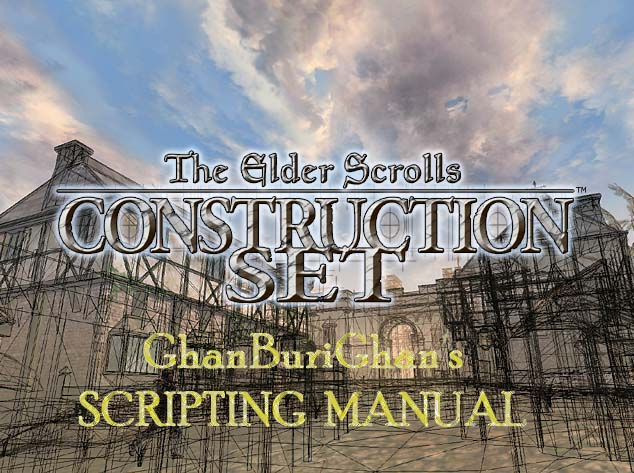
\includegraphics{media/image1.jpg}

\clearpage

\tableofcontents
\addtocontents{toc}

%Table of Contents
%
%\protect\hyperlink{foreword-to-the-ninth-edition}{Foreword to the ninth
%edition 9}
%
%\protect\hyperlink{foreword-to-eighth-edition}{Foreword to eighth
%edition 10}
%
%\protect\hyperlink{_Toc53412549}{Introduction 11}
%
%\protect\hyperlink{using-this-guide.}{Using this guide. 11}
%
%\protect\hyperlink{what-is-a-script}{What is a script? 11}
%
%\protect\hyperlink{what-can-scripts-do}{What can scripts do? 12}
%
%\protect\hyperlink{what-scripts-cant-do}{What scripts can't do: 12}
%
%\protect\hyperlink{_Toc53412554}{Scripting tutorial 13}
%
%\protect\hyperlink{lets-get-going}{Let's get going! 13}
%
%\protect\hyperlink{the-scripting-window}{The scripting window 13}
%
%\protect\hyperlink{what-do-we-want}{What do we want? 14}
%
%\protect\hyperlink{writing-a-script}{Writing a script 14}
%
%\protect\hyperlink{naming-a-script-begin-and-end}{Naming a script: Begin
%and End 14}
%
%\protect\hyperlink{detecting-an-action-by-the-player}{Detecting an
%action by the player 15}
%
%\protect\hyperlink{writing-text-and-obtaining-decisions-from-the-player}{Writing
%text and obtaining decisions from the player 15}
%
%\protect\hyperlink{how-local-scripts-are-executed}{How local scripts are
%executed 16}
%
%\protect\hyperlink{your-first-bug}{Your first bug 19}
%
%\protect\hyperlink{putting-a-spell-on-the-player}{Putting a spell on the
%player 19}
%
%\protect\hyperlink{how-to-learn-more}{How to learn more 22}
%
%\protect\hyperlink{general-information-scripts-commands-and-syntax}{General
%Information: Scripts, Commands and Syntax 23}
%
%\protect\hyperlink{types-of-scripts}{Types of scripts 23}
%
%\protect\hyperlink{local-scripts}{Local scripts 23}
%
%\protect\hyperlink{global-scripts}{Global scripts 23}
%
%\protect\hyperlink{syntax}{Syntax 25}
%
%\protect\hyperlink{beginning-and-ending-scripts}{Beginning and ending
%scripts 25}
%
%\protect\hyperlink{general-syntax-for-functions}{General syntax for
%functions: 25}
%
%\protect\hyperlink{general-syntax-commas-parentheses-and-spaces}{General
%syntax: Commas, parentheses and spaces 26}
%
%\protect\hyperlink{comments}{Comments 26}
%
%\protect\hyperlink{indentation-using-tabstops}{Indentation / using
%tabstops 26}
%
%\protect\hyperlink{variables}{Variables 27}
%
%\protect\hyperlink{types-of-variables}{Types of variables 27}
%
%\protect\hyperlink{_Toc182634499}{Local variables 28}
%
%\protect\hyperlink{global-variables}{Global variables 29}
%
%\protect\hyperlink{referencing-variables-on-other-objects-and-scripts}{Referencing
%variables on other objects and scripts 29}
%
%\protect\hyperlink{using-variables-in-functions}{Using variables in
%functions 30}
%
%\protect\hyperlink{section}{Operators / mathematical calculations 30}
%
%\protect\hyperlink{_Toc182634504}{Testing conditions 31}
%
%\protect\hyperlink{use-of-if-elseif-conditions}{Use of if\ldots{} elseif
%conditions 31}
%
%\protect\hyperlink{while-conditions}{While conditions 33}
%
%\protect\hyperlink{constructing-boolean-operations-in-tes-script}{Constructing
%Boolean operations in TES Script 34}
%
%\protect\hyperlink{_Toc53412583}{List of TES-script functions 35}
%
%\protect\hyperlink{explanation-of-the-format}{Explanation of the format
%35}
%
%\protect\hyperlink{working-with-objects}{Working with objects 36}
%
%\protect\hyperlink{working-with-inventory-items}{Working with inventory
%items 36}
%
%\protect\hyperlink{adding-and-removing-items-from-the-inventory}{Adding
%and removing items from the inventory 36}
%
%\protect\hyperlink{dropping-items-to-the-floor}{Dropping items to the
%floor 38}
%
%\protect\hyperlink{monitoring-inventory-activities-adding-dropping-items-and-using-soul-gems}{Monitoring
%inventory activities: Adding, dropping items and using soul gems 39}
%
%\protect\hyperlink{force-equipping-an-item}{Force-equipping an Item 40}
%
%\protect\hyperlink{detecting-if-an-item-has-been-equipped}{Detecting if
%an item has been equipped 41}
%
%\protect\hyperlink{disabling-ability-to-equip-an-item}{Disabling ability
%to equip an item 42}
%
%\protect\hyperlink{_Toc182634518}{Checking for presence of items in
%inventory 43}
%
%\protect\hyperlink{repairing-objects}{Repairing objects 43}
%
%\protect\hyperlink{worn-equipped-object-information}{Worn / equipped
%object information 43}
%
%\protect\hyperlink{usedonme-function}{UsedOnMe function 46}
%
%\protect\hyperlink{moving-and-placing-objects}{Moving and placing
%objects 46}
%
%\protect\hyperlink{moving-along-an-objects-axis}{Moving along an objects
%axis 46}
%
%\protect\hyperlink{moving-along-the-world-axis}{Moving along the world
%axis 47}
%
%\protect\hyperlink{cellupdate}{CellUpdate 48}
%
%\protect\hyperlink{setting-position-the-other-way-to-do-movement}{Setting
%position (the other way to do movement) 48}
%
%\protect\hyperlink{positioning-an-object-in-the-world-or-in-an-interior-cell}{Positioning
%an object in the world or in an interior cell 50}
%
%\protect\hyperlink{resetting-an-object-to-its-original-position}{Resetting
%an object to its original position 51}
%
%\protect\hyperlink{placing-an-item-near-the-pc}{Placing an item near the
%PC 51}
%
%\protect\hyperlink{place-items-near-an-object}{Place items near an
%object 52}
%
%\protect\hyperlink{creating-new-object-references-with-placeitem}{Creating
%new object-references with PlaceItem 52}
%
%\protect\hyperlink{rotation-and-angles}{Rotation and angles 54}
%
%\protect\hyperlink{making-an-object-spin}{Making an object spin 54}
%
%\protect\hyperlink{setting-angles}{Setting Angles 54}
%
%\protect\hyperlink{scale-functions}{Scale Functions 56}
%
%\protect\hyperlink{determining-location-relative-position-and-movement}{Determining
%location, relative position and movement 58}
%
%\protect\hyperlink{detecting-if-player-is-indoors-or-outdoors}{Detecting
%if player is indoors or outdoors 58}
%
%\protect\hyperlink{determining-the-players-cell}{Determining the players
%cell 58}
%
%\protect\hyperlink{distance-of-one-object-to-another}{Distance of one
%object to another 59}
%
%\protect\hyperlink{determining-an-objects-position-and-facing}{Determining
%an objects position and facing 59}
%
%\protect\hyperlink{line-of-sight}{Line of Sight 60}
%
%\protect\hyperlink{_Toc182634542}{Determine whether an Actor is detected
%by another Actor 62}
%
%\protect\hyperlink{determining-when-the-pc-leaves-a-cell}{Determining
%when the PC leaves a cell 62}
%
%\protect\hyperlink{detect-player-traveling}{Detect player traveling 63}
%
%\protect\hyperlink{triggers-for-actors-standing-on-an-object}{Triggers
%for Actors standing on an object 64}
%
%\protect\hyperlink{hurting-an-actor-standing-on-an-object}{Hurting an
%Actor standing on an object 65}
%
%\protect\hyperlink{_Toc182634547}{Object Collision Functions 65}
%
%\protect\hyperlink{checking-activation-of-an-item-and-activating-it}{Checking
%activation of an item and activating it 66}
%
%\protect\hyperlink{locking-and-unlocking-doors-or-chests}{Locking and
%Unlocking doors or chests 69}
%
%\protect\hyperlink{animating-objects}{Animating objects 69}
%
%\protect\hyperlink{enabling-and-disabling-objects}{Enabling and
%disabling objects 71}
%
%\protect\hyperlink{deleting-a-reference-completely}{Deleting a reference
%completely 72}
%
%\protect\hyperlink{dont-save-changes-to-an-object}{Don't save changes to
%an object 74}
%
%\protect\hyperlink{scripting-npcs-ai-and-movement}{Scripting NPC's: AI
%and Movement 75}
%
%\protect\hyperlink{make-an-npc-walk-to-a-new-location}{Make an NPC walk
%to a new location 75}
%
%\protect\hyperlink{checking-whether-an-npc-has-performed-his-movement}{Checking
%whether an NPC has performed his movement 75}
%
%\protect\hyperlink{make-an-actor-turn-or-face-a-certain-direction}{Make
%an Actor turn or face a certain direction 77}
%
%\protect\hyperlink{define-random-actor-movement}{Define random Actor
%movement 77}
%
%\protect\hyperlink{making-actors-activate-objects}{Making Actors
%activate objects 79}
%
%\protect\hyperlink{following-and-escorting}{Following and Escorting 80}
%
%\protect\hyperlink{checking-which-ai-package-is-currently-executed}{Checking
%which AI package is currently executed 81}
%
%\protect\hyperlink{forcing-sneak-movement}{Forcing sneak movement 83}
%
%\protect\hyperlink{forcing-running-and-jumping-tribunal-npc-movement-functions}{Forcing
%running and jumping: Tribunal NPC Movement Functions 85}
%
%\protect\hyperlink{detecting-players-action-running-jumping-sneaking}{Detecting
%players action: running, jumping, sneaking? 86}
%
%\protect\hyperlink{detect-combat-readiness}{Detect combat readiness 87}
%
%\protect\hyperlink{section-7}{Making someone fall 88}
%
%\protect\hyperlink{equipment-sharing-and-other-companion-functions}{Equipment
%sharing and other companion functions 88}
%
%\protect\hyperlink{race-faction-and-rank}{Race, Faction and Rank 90}
%
%\protect\hyperlink{determining-race}{Determining Race 90}
%
%\protect\hyperlink{determining-the-pcs-faction-status}{Determining the
%PC's Faction status: 90}
%
%\protect\hyperlink{modifying-faction-standing-and-reaction}{Modifying
%faction standing and reaction 91}
%
%\protect\hyperlink{determining-and-changing-reputation-and-disposition}{Determining
%and changing reputation and disposition 93}
%
%\protect\hyperlink{werewolf-specific-functions}{Werewolf-specific
%functions 94}
%
%\protect\hyperlink{set-the-werewolf-attributes}{Set the werewolf
%attributes 94}
%
%\protect\hyperlink{change-the-color-of-secunda}{Change the color of
%Secunda 94}
%
%\protect\hyperlink{determine-how-many-kills-a-werewolf-has}{Determine
%how many kills a werewolf has 94}
%
%\protect\hyperlink{check-to-see-if-the-creature-is-in-werewolf-form}{Check
%to see if the creature is in werewolf form 95}
%
%\protect\hyperlink{change-to-a-werewolf}{Change to a werewolf 95}
%
%\protect\hyperlink{section-8}{Special werewolf global variables 96}
%
%\protect\hyperlink{text-and-dialogue}{Text and Dialogue 97}
%
%\protect\hyperlink{brief-dialogue-how-to}{Brief dialogue how-to 97}
%
%\protect\hyperlink{the-concept-of-mw-dialogue}{The concept of MW
%dialogue 97}
%
%\protect\hyperlink{how-dialogue-works}{How dialogue works 98}
%
%\protect\hyperlink{a-few-golden-rules}{A few golden rules 101}
%
%\protect\hyperlink{dialogue-101}{Dialogue 101 101}
%
%\protect\hyperlink{dialogue-related-functions}{Dialogue-related
%functions 103}
%
%\protect\hyperlink{displaying-messages}{Displaying messages 103}
%
%\protect\hyperlink{_Toc182634588}{Displaying variables and text defines
%in a message box 105}
%
%\protect\hyperlink{adding-a-dialogue-topic}{Adding a dialogue topic 106}
%
%\protect\hyperlink{initiating-and-ending-dialogue}{Initiating and ending
%dialogue 107}
%
%\protect\hyperlink{allowing-forced-dialogue-with-werewolf-player-bloodmoon}{Allowing
%forced Dialogue with Werewolf player (Bloodmoon) 108}
%
%\protect\hyperlink{multiple-choice-asking-questions}{Multiple choice --
%asking questions 109}
%
%\protect\hyperlink{adding-to-the-journal-and-testing-journal-entries}{Adding
%to the journal and testing journal entries 110}
%
%\protect\hyperlink{special-dialogue-only-functions}{Special
%dialogue-only functions 111}
%
%\protect\hyperlink{changing-the-hello-setting}{Changing the Hello
%setting 112}
%
%\protect\hyperlink{useful-dialogue-variables}{Useful dialogue variables
%112}
%
%\protect\hyperlink{changing-and-testing-skills-attributes-and-other-stats}{Changing
%and testing Skills, Attributes, and other Stats 113}
%
%\protect\hyperlink{get-set-and-modify-stats---general-remarks}{Get, Set,
%and Modify stats - general remarks 113}
%
%\protect\hyperlink{determining-and-changing-actor-and-player-stats}{Determining
%and changing Actor and player stats: 114}
%
%\protect\hyperlink{determining-and-changing-attributes}{Determining and
%changing Attributes: 114}
%
%\protect\hyperlink{determining-and-changing-health-magicka-fatigue}{Determining
%and changing Health, Magicka, Fatigue: 114}
%
%\protect\hyperlink{determining-and-changing-skills}{Determining and
%changing Skills: 115}
%
%\protect\hyperlink{determining-and-changing-level}{Determining and
%changing Level 115}
%
%\protect\hyperlink{_Toc182634604}{GetStat, ModStat and SetStat: A
%concerned modder's guide. - Galsiah 116}
%
%\protect\hyperlink{combat}{Combat 120}
%
%\protect\hyperlink{initiating-and-ending-combat}{Initiating and ending
%combat 120}
%
%\protect\hyperlink{detecting-attack}{Detecting Attack 120}
%
%\protect\hyperlink{combat-related-getmodset-ai-functions-fight-flee-alarm}{Combat
%related Get/Mod/Set AI functions: Fight, Flee, Alarm 122}
%
%\protect\hyperlink{keeping-track-of-kills-and-knockouts}{Keeping track
%of kills and knockouts 123}
%
%\protect\hyperlink{resurrecting-a-dead-actor}{Resurrecting a dead Actor
%125}
%
%\protect\hyperlink{crime}{Crime 126}
%
%\protect\hyperlink{determining-and-changing-crime-level}{Determining and
%changing Crime Level 126}
%
%\protect\hyperlink{jailing-the-pc}{Jailing the PC 126}
%
%\protect\hyperlink{clearing-the-pc-of-crime}{Clearing the PC of crime
%126}
%
%\protect\hyperlink{detecting-crime}{Detecting crime 126}
%
%\protect\hyperlink{useful-global-variables}{Useful global variables 128}
%
%\protect\hyperlink{magic}{Magic 129}
%
%\protect\hyperlink{limiting-the-use-of-teleport}{Limiting the use of
%teleport 129}
%
%\protect\hyperlink{limiting-the-use-of-levitation}{Limiting the use of
%levitation 130}
%
%\protect\hyperlink{checking-and-managing-souls-and-soulgems}{Checking
%and managing souls and soulgems 131}
%
%\protect\hyperlink{adding-and-removing-spells-and-cursing}{Adding and
%removing spells and cursing 133}
%
%\protect\hyperlink{casting-spells}{Casting spells 134}
%
%\protect\hyperlink{managing-and-testing-for-spells}{Managing and testing
%for spells 135}
%
%\protect\hyperlink{managing-and-testing-spell-effects}{Managing and
%testing spell effects 136}
%
%\protect\hyperlink{testing-disease}{Testing disease 137}
%
%\protect\hyperlink{explosion}{Explosion 138}
%
%\protect\hyperlink{magic-getmodset-effects-functions}{Magic Get/Mod/Set
%effects functions: 138}
%
%\protect\hyperlink{sound}{Sound 140}
%
%\protect\hyperlink{make-actors-speak-an-audio-file}{Make Actors speak an
%audio file 140}
%
%\protect\hyperlink{playing-music}{Playing music 140}
%
%\protect\hyperlink{playing-sounds}{Playing sounds 141}
%
%\protect\hyperlink{controlling-sound}{Controlling sound 141}
%
%\protect\hyperlink{sound-file-formats}{Sound file formats 142}
%
%\protect\hyperlink{keeping-track-of-time}{Keeping track of time 143}
%
%\protect\hyperlink{timer}{Timer 143}
%
%\protect\hyperlink{morrowinds-time-related-global-variables}{Morrowind's
%time related global variables 143}
%
%\protect\hyperlink{keeping-track-of-days-passed}{Keeping track of days
%passed 144}
%
%\protect\hyperlink{moon-phases}{Moon phases 144}
%
%\protect\hyperlink{weather}{Weather 146}
%
%\protect\hyperlink{changing-weather}{Changing weather 146}
%
%\protect\hyperlink{changing-weather-settings-for-a-region}{Changing
%weather settings for a region 146}
%
%\protect\hyperlink{determining-current-weather}{Determining current
%weather 147}
%
%\protect\hyperlink{detecting-wind-speed}{Detecting wind speed 147}
%
%\protect\hyperlink{player-sleeping}{Player sleeping 148}
%
%\protect\hyperlink{enabling-and-disabling-player-control-and-interface}{Enabling
%and disabling player control and interface 149}
%
%\protect\hyperlink{disable-player-control-functions}{Disable player
%control functions 149}
%
%\protect\hyperlink{enable-player-control-functions}{Enable player
%control functions 149}
%
%\protect\hyperlink{check-player-control-status}{Check player control
%status 150}
%
%\protect\hyperlink{force-first-or-third-person-view}{Force first or
%third person view 150}
%
%\protect\hyperlink{functions-for-character-generation-menus}{Functions
%for character generation menus 150}
%
%\protect\hyperlink{determining-if-player-has-menus-open}{Determining if
%player has menus open 151}
%
%\protect\hyperlink{using-menutest-to-open-and-close-menus}{Using
%MenuTest to open and close menus 152}
%
%\protect\hyperlink{miscellaneous-functions-and-variables}{Miscellaneous
%functions and variables 153}
%
%\protect\hyperlink{breaking-of-script-processing}{Breaking of script
%processing 153}
%
%\protect\hyperlink{controlling-global-scripts}{Controlling global
%scripts 153}
%
%\protect\hyperlink{fading-the-screen-in-and-out}{Fading the screen in
%and out 154}
%
%\protect\hyperlink{adding-a-location-to-the-map}{Adding a location to
%the map 154}
%
%\protect\hyperlink{assigning-random-values-to-variables}{Assigning
%random values to variables 154}
%
%\protect\hyperlink{playing-videos}{Playing videos 155}
%
%\protect\hyperlink{_Toc182634660}{Levelled List functions 156}
%
%\protect\hyperlink{square-root}{Square root 157}
%
%\protect\hyperlink{water-level-functions}{Water Level Functions 157}
%
%\protect\hyperlink{tips-and-tricks}{Tips and tricks 160}
%
%\protect\hyperlink{little-helpers-text-search-copy-paste}{Little
%helpers: Text search, copy, paste 160}
%
%\protect\hyperlink{alternative-scripting-editors}{Alternative scripting
%editors 160}
%
%\protect\hyperlink{script-extenders}{Script Extenders 161}
%
%\protect\hyperlink{script-with-style-for-safer-scripting}{Script with
%style for safer scripting 162}
%
%\protect\hyperlink{cleaning-up-your-mod}{Cleaning up your mod 163}
%
%\protect\hyperlink{on-references-persist}{On References Persist 165}
%
%\protect\hyperlink{the-72-hours-bug-a-brief-explanation}{The "72-Hours
%Bug": A Brief Explanation 165}
%
%\protect\hyperlink{limits-of-the-script-editor}{Limits of the Script
%Editor 166}
%
%\protect\hyperlink{pitfalls}{Pitfalls 167}
%
%\protect\hyperlink{saving-cpu-time}{Saving CPU time 168}
%
%\protect\hyperlink{targeted-scripts-running-global-scripts-tied-to-an-object}{Targeted
%scripts: running "global" scripts tied to an object 170}
%
%\protect\hyperlink{detecting-when-the-player-does-a-load-from-saved-game}{Detecting
%when the player does a load from saved game: 171}
%
%\protect\hyperlink{uses-of-the-chargenstate-variable---disabling-saving-and-menus}{Uses
%of the CharGenState variable - Disabling saving and menus 173}
%
%\protect\hyperlink{detecting-use-of-scrolls-or-books}{Detecting use of
%scrolls or books 174}
%
%\protect\hyperlink{making-actors-switch-between-weapons}{Making Actors
%switch between weapons 176}
%
%\protect\hyperlink{_Toc182634679}{Making NPCs switch between spell
%"sets" 177}
%
%\protect\hyperlink{making-actors-lie-down}{Making Actors lie down 177}
%
%\protect\hyperlink{scripted-teleporting}{Scripted teleporting 181}
%
%\protect\hyperlink{interaction-between-mods}{Interaction between mods
%183}
%
%\protect\hyperlink{safely-starting-global-scripts--avoiding-the-main-script}{Safely
%starting global scripts- avoiding the main script 184}
%
%\protect\hyperlink{use-sound-to-detect-events}{Use sound to detect
%events 185}
%
%\protect\hyperlink{large-battles}{Large battles 185}
%
%\protect\hyperlink{a-guide-to-making-ridable-objects}{A guide to making
%ridable objects 186}
%
%\protect\hyperlink{selecting-objects}{Selecting objects 186}
%
%\protect\hyperlink{creatingdeleting-objects}{Creating/Deleting objects
%186}
%
%\protect\hyperlink{falling-off-from-objects}{Falling off from objects
%187}
%
%\protect\hyperlink{collision-detection}{Collision detection 188}
%
%\protect\hyperlink{savegame-issue}{Savegame issue 188}
%
%\protect\hyperlink{trigonometry-script---fast-sine-and-cosine}{Trigonometry
%script - fast sine and cosine 189}
%
%\protect\hyperlink{mannequins}{Mannequins 198}
%
%\protect\hyperlink{is-she-looking-at-me}{Is she looking at me? 201}
%
%\protect\hyperlink{cinematic-sequence}{Cinematic sequence 203}
%
%\protect\hyperlink{troubleshooting}{Troubleshooting 204}
%
%\protect\hyperlink{general-hints}{General hints 204}
%
%\protect\hyperlink{the-console}{The Console 204}
%
%\protect\hyperlink{using-the-console-to-check-variables}{Using the
%Console to check variables: 204}
%
%\protect\hyperlink{using-the-console-to-quickly-test-scripts}{Using the
%Console to quickly test scripts: 204}
%
%\protect\hyperlink{error-messages-malfunctions-and-common-causes}{Error
%messages, malfunctions and common causes 205}
%
%\protect\hyperlink{in-the-editor}{In the editor 205}
%
%\protect\hyperlink{in-game-error-messages}{In game error messages: 205}
%
%\protect\hyperlink{appendix}{Appendix 208}
%
%\protect\hyperlink{new-functions-that-come-with-tribunal}{New functions
%that come with TRIBUNAL 208}
%
%\protect\hyperlink{changes-fixes-to-morrowind-scripting}{Changes / fixes
%to Morrowind scripting: 208}
%
%\protect\hyperlink{index-of-new-tribunal-script-functions}{Index of new
%Tribunal Script Functions: 208}
%
%\protect\hyperlink{new-functions-that-come-with-bloodmoon}{New functions
%that come with BLOODMOON 209}
%
%\protect\hyperlink{index-of-new-bloodmoon-script-functions-and-variables}{Index
%of new Bloodmoon Script Functions and variables: 209}
%
%\protect\hyperlink{previously-undocumented-functions}{Previously
%undocumented functions 210}
%
%\protect\hyperlink{variable-type-functions}{Variable-type functions:
%211}
%
%\protect\hyperlink{local-variables-that-get-set-by-the-game}{Local
%variables that get set by the game: 211}
%
%\protect\hyperlink{local-variables-that-you-can-set-as-a-flag}{Local
%variables that you can set as a flag: 211}
%
%\protect\hyperlink{special-globals}{Special Globals 211}
%
%\protect\hyperlink{game-units}{Game units: 213}
%
%\protect\hyperlink{derived-attribute-calculations}{Derived attribute
%calculations: 213}
%
%\protect\hyperlink{_Toc53412751}{Magic Effect List 215}
%
%\protect\hyperlink{list-of-console-commands}{List of console commands
%216}
%
%\protect\hyperlink{game-settings}{Game Settings 219}
%
%\protect\hyperlink{index}{Index 226}

\hypertarget{foreword-to-the-tenth-edition}{%
\subsubsection{\texorpdfstring{\hfill\break
Foreword to the tenth edition}{Foreword to the ninth edition}}\label{foreword-to-the-tenth-edition}}

This community edition is a port to LaTeX for easy and open collaboration. Development is at https://github.com/sultan-of-rum/morrowind-scripting-for-dummies. Please send all bug reports to this repository.

The primary focus for this project is to incorporate corrections and updates by the Tamriel Rebuilt team. Special thanks goes to them for allowing free use of their information. It also uses default OpenMW-CS syntax highlighting, and a main goal is to move towards an open license.

\hypertarget{foreword-to-the-ninth-edition}{%
\subsubsection{\texorpdfstring{\hfill\break
Foreword to the ninth edition}{Foreword to the ninth edition}}\label{foreword-to-the-ninth-edition}}

Another update, this time by more than one person, now you can get really confused when it mentions that ``I'' did something or found something *grins*. Although this update was intended as a bugfix, a huge amount of new information has been added - since much of it concerns the bugs and pitfalls of the scripting language that have been discovered since version 8, you will find changes and additions scattered throughout.

I have also added a couple more functions that were missing from the last version, and there is a small section on script extenders to give a brief overview of what can be done with each which should hopefully prove informative to anyone wanting to know more about what they do. Galsiah proveded a large section on the failings of get/mod/set stat; there is a lot more info on dialog and how it works, which should be very useful; a short explanation of float values and how they work has
been added; some sections have been rearranged for clarity; and I \emph{think} I've removed all the en dashes and typographer's quotes from code blocks, so it should be safe to copy-paste most of the example scripts now.

Special thanks go to GhanBuriGhan, who gave me permission to update his indispensable guide. Also thanks to Dave Humphrey for his permission to use the information on UESP wiki, and everyone who contributed to that wiki. I would like to thank exclusiveor77, DinkumThinkum, Björn, abot, Galsiah, Casey Tucker, cyran0 and JOG for the huge amount of information they gave me on the forums.

However without the help of the rest of community, everyone who collected all the information, posted their experiences, this guide would have never happened.

Yacoby and melian

\hypertarget{foreword-to-eighth-edition}{%
\subsubsection{\texorpdfstring{\hfill\break
Foreword to eighth edition}{ Foreword to eighth edition}}\label{foreword-to-eighth-edition}}

Oh no, MSFD updates again! Quite a few changes this time. I have continued to reorder functions to achieve a more consistent classification. In the course of this restructuring of the text, Tribunal and Bloodmoon functions are now also sorted among the rest of the functions (but clearly marked), and the same applies for Get/Set/ModStat type functions - the ones that affect magic are now in the Magic section, the ones that affect combat are in the combat chapter, and so on. I reformatted all the function entries for better visibility. There are also a good number of corrections and additions: check out the corrected list of idles in AIWander, more detailed info on functions such as OnDeath, OnActivate, or the revelation that some functions, like PositionCell use a different unit for the angle setting (minutes instead of degrees). There is a lot of interesting new detail on the intricacies of RemoveItem, OnPCEquip, and SkipEquip. Throughout, I have added a couple more sample scripts. I have assembled a tips list on Dialogue from the information from a once-pinned thread on the official forums. To make your mod-testing easier, I now have a much more complete list of console commands, and you may find that some of these may actually be useful script functions as well. A nice collection of new tips and tricks have also been added, e.g. on how to detect savegame loading, alternative script editors, a fast sine and cosine calculator and more.

I would like to mention something here, that has become more and more evident in recent discussions. Apparently the different versions of the game (Morrowind, the expansions, various updates, European/American versions), have quite a number of functional differences with respect to scripting. This may explain a lot of the conflicting information I get about some functions. Some functions actually seem to have lost functionality in later versions of the game, some regained functionality, etc. In the absence of a full change log by Bethesda it is unfortunately impossible to really give a final verdict in many of these cases.

Again I can only stress that this guide would never have become what it is without the help and support of the modding community. This time, I would like to say special thanks to Nigedo, DinkumThinkum, ManaUser, ThePal, Erstam, JDGBOLT, Klinn, and MentalElf, for their tireless help in finding and solving many errors or inconsistencies in the last edition, or sharing scripts and information with me. Thanks also to Emma, for all the info she put into that dialogue thread on the forums.

GhanBuriGhan

Disclaimer \& Copyright Statment: The Elder Scrolls, Morrowind, Daggerfall, Arena, Tribunal, Bloodmoon the TES Construction Set etc. are property of Bethesda Softworks, a ZeniMax Media company. The authors and editors of this manual make no claims to these names and trademarks. In all other respects I (GhanBuriGhan) maintain the copyright for this document. This guide is fully unofficial and in no way am I, any other authors or editors, or Bethesda responsible for any damages or loss of data, patience, hair, or sanity inflicted through the use of this manual. You can freely distribute this document as long as you keep it intact and unmodified.

\emph{\textbf{If you find older versions of this document on the web for
download, please inform the webmaster about the new version.}}

% Chapter sectioning
%\protect\hypertarget{_Toc53412549}{}{}

\section{Introduction}

\hypertarget{using-this-guide.}{%
\subsection{Using this guide.}\label{using-this-guide.}}

If you are new to scripting, you should probably start by reading this introduction and especially do the tutorial. It is my best attempt at explaining scripts, what they do, and how to program one, in simple terms.

Secondly this is a manual, a reference, a handbook. The bulk of this document is a documentation of the available functions. This part is not written for the beginner, you are expected to know the basics of scripting already. I have however tried to provide a lot more info, explanations and sample scripts than the original helpfile, to make it easier to use these functions correctly in your scripts. Use the index at the end of the document to find info on a specific function, or the table of contents to find functions related to a general area of
interest. If you run into errors, the Troubleshooting section may help you a bit. In the Appendix you find lists that may also come in handy as a reference.

Thirdly, as an advanced scripter you may find the Tips and Tricks section interesting that covers both basic advice and advanced scripting techniques.

Finally a word of advice: don't take what's written here as gospel. The info in this guide represents the best of my knowledge and forum wisdom, but that doesn't mean that there aren't mistakes and oversights, etc. E.g. if I write that a function doesn't take variables as arguments it \emph{probably} doesn't -- but if it is important for your mod, by all means try anyway. It may have changed with a patch or maybe simply nobody checked before. So run a test, and if you find something new, let me know, and I will add the info in a possible future update.

\hypertarget{what-is-a-script}{%
\subsection{What is a script?}\label{what-is-a-script}}

Scripts are basically pieces of code written in a special scripting language (I will call it TES script from here on). These little "programs" will run during the game and can perform certain things in the game, lots of things actually: Trigger events, control time and place, make things and creatures vanish, appear or move, give messages to the player, change stats, even change the weather -- the possibilities are great.

TES Script is a unique scripting language, it is not used outside the TES Construction Set. As a scripting language it has certain limitations compared to a "real" programming language, like, e.g. C++:

\begin{enumerate}
\def\labelenumi{\arabic{enumi}.}
\item
  The scope of TES Script is limited-- don't expect to be able to program anything that is not already in the game in one way or another -- which is not to say you can not achieve new and unusual things with scripting! But you can't use TES script to, say, program a word processor.
\item
  TES Script is also not an SDK (software development kit) that lets you actually work with and change (parts of) the games source code. That's why you can't use TES script to, for example, add new weather-effects. Those are hardcoded and you would need to change the actual game .exe to do that.
\item
  It's an interpreted language not a compiled one -- the code needs a separate program (in this case Morrowind) to run -- unlike compiled code that could be run by itself, like an .exe application.
\end{enumerate}

\hypertarget{what-can-scripts-do}{%
\subsection{What can scripts do?}\label{what-can-scripts-do}}

Scripts for Morrowind are a way to have the game dynamically react to what the player does in the game world. You can use scripts to manage complex quests. You can use scripts to create custom items that perform actions beyond what regular enchantments could. You can use scripts to create traps. You can use scripts to change NPC or creature behavior. Remember the character creation in Morrowind? It's basically controlled by a number of scripts. Seen Fargoth sneak around to his stash in Seyda Neen? That's a script directing his moves. Freed any slaves? That also is handled by a script. So the short answer to the question is: a lot.

\hypertarget{what-scripts-cant-do}{%
\subsection{What scripts can't do:}\label{what-scripts-cant-do}}

The TES script language is limited in its capabilities -- there are only so many functions that you can use and sometimes the possible uses are not all that you may wish them to be. In fact some functions are buggy or plain broken. In many cases smart scripters can find workarounds for apparent limitations, but don't expect miracles. Many things are hardcoded and can not or only indirectly be influenced by scripts.

% End text.

% Chapter sectioning]
%\protect\hypertarget{_Toc53412554}{}{}
\section{Scripting tutorial}

If you are completely new to scripting and programming in general, the thought of using TES script might be a little daunting -- I have therefore written an extended tutorial that will walk you through making your first script. I will also explain the main elements of the scripting language as we go. There will be other explanations on the way, but the key instructions will be in \textbf{bold} print.

\hypertarget{lets-get-going}{%
\subsection{Let's get going!}\label{lets-get-going}}

We start by opening the script editor: \textbf{Start up the TES Construction Set, open the Morrowind.esm file and then select Edit Scripts from the Gameplay menu to open the scripting window.}

\hypertarget{the-scripting-window}{%
\subsection{The scripting window}\label{the-scripting-window}}

You enter the script editor either by \textbf{selecting Gameplay -- Edit Scripts from the menu}, by clicking the edit script button (the pencil) in the taskbar or by accessing it from an Object or NPC dialogue, by clicking the button with the ellipses {[}\ldots{]} next to the script field. The editor window is pretty basic:

% Graphic here is on another page because the margins are different than the .doc

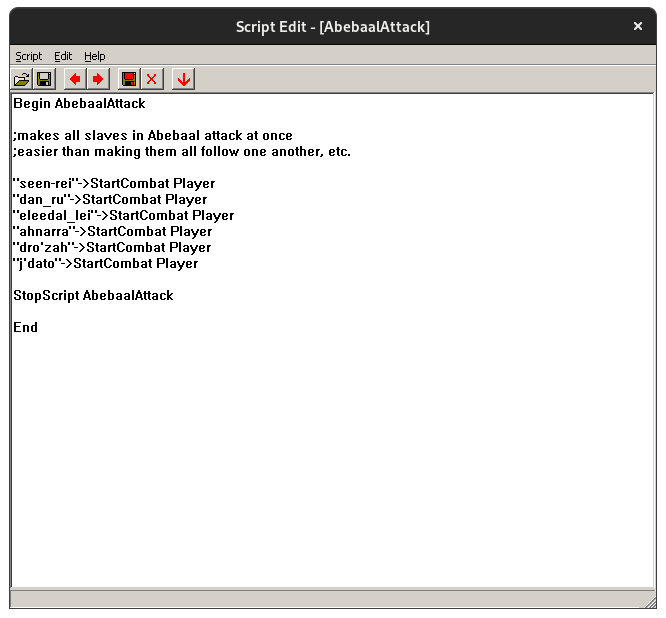
\includegraphics{media/script-abebaal-attack.png}

Let's have a look at the buttons in the taskbar, from left to right: \emph{Open} lets you select a script to edit. \emph{Save} error checks the current script and compiles it or gives out error messages -- note, however, that the plugin and thus the script is not really saved to disk at this time. When programming large scripts frequently use the save command in the main TESCS window after you have saved the script here, just in case the TESCS crashes.

Note that if you edit the script and suddenly hit "save plugin" to backup in the middle of the work, your updated script will NOT be saved with it. You must save it manually first. Also, if you just close script window, it doesn't mean that script will be saved. You must take care of it yourself (Thanks to Kir for this tip).

\emph{Forward and Backward arrows} jump to the next or previous script, respectively (alphabetical order). If you give your scripts a common tag, that will make it easier to jump between the different scripts of your project, e.g. start every script name with AA\_Scriptname this will put them right at the beginning of the list and keep them neatly together. \emph{Compile all} recompiles all scripts (what's this good for? I don't really know). Finally, the \emph{delete} button deletes a script and the last "\emph{arrow down}" button closes the script window.

The help menu gives quick access to the function and command pages of the helpfile (of moderate utility, hence the creation of this manual!)

You can cut, copy, and paste from and into the editor window by using the Windows standards ctrl-c for copy, ctrl-x for cut and ctrl-v for paste.

\hypertarget{what-do-we-want}{%
\subsection{What do we want?}\label{what-do-we-want}}

Before we really start writing our tutorial script we should decide what we want it to do. For this tutorial I decided we are going to make a \textbf{Riddle Chest: The chest will ask a riddle and only the right answer will open the chest. If the player provides the wrong answer, a trap will go off, hurting the player, and the chest can't be opened.}

That's a fairly complex undertaking, but we will take it step by step.

\hypertarget{writing-a-script}{%
\subsection{Writing a script}\label{writing-a-script}}

Ok, once you've got the Edit Script window open, \textbf{click into the main part of the window.} That is where you will write your script.

\hypertarget{naming-a-script-begin-and-end}{%
\subsubsection{Naming a script: Begin and End}\label{naming-a-script-begin-and-end}}

First of all we must give our script a name -- every script must start with the declaration of this name. \textbf{So please type:}

\begin{lstlisting}
Begin my_first_script
\end{lstlisting}

\textbf{into the editor window}. Note the underscores: Your name should be one word. Also note that the script language is not case sensitive, so \emph{Begin} could also be written without the capital letter: \emph{begin}. This name is the handle by which the script will be known in the TESCS. Try hitting the save button now: you will get an error message about "you need to end your script with end scriptname. So, for the editor to recognize the script we also need to indicate an
end: \textbf{next, write}

\begin{lstlisting}
End
\end{lstlisting}

\textbf{in a new line below the above}. As you see we can omit putting the name of the script in this line again, just \emph{end} will do. When you hit \emph{safe} now, you will see the name appear in the title bar of the script editor, indicating that the script has been accepted. This is the shortest script possible - and of course it doesn't do anything at all.

\hypertarget{detecting-an-action-by-the-player}{%
\subsubsection{Detecting an action by the player}\label{detecting-an-action-by-the-player}}

Next, we need a way to determine whether the player tries to open the chest. In TES Script we distinguish between Objects, Functions and Commands --

\textbf{Objects} are all the things in the game world, be they visible objects, creatures, NPCs or just sounds.

\textbf{Functions} are the all the "words" of TES Script that let us either manipulate these objects or let us gather information about them.

\textbf{Commands} are those "words" that structure the scripting language, but do not operate on any Game objects -- an example is the word "Begin" we used to tell the script editor about the name of our script.

To tell the game which object it is supposed to perform a given function on we can use the "arrow", or "fix" : -> (really just a hyphen and a greater-than sign). You specify the object for the function on the left (we also call this the calling object) and the function to be performed on the right:

Object\_ID-> function, {[}parameters{]}

A function may or may not have parameters. Parameters could be other object ID's, numbers and in some cases, variables.

What we need for our riddle chest is the OnActivate function: this is an informative function that tells us whether the player has "activated" an object in the game world or not. This function returns a value of 1 (which means "true" in programming terms) if the object has been activated, that means the player targets it and presses the "use" button (space, by default). So what we need to do is check if OnActivate becomes "true" anytime in the game. \textbf{So edit your script to look like this:}

\lstinputlisting{scripts/my_first_script01.txt}

A couple more things need to be explained here: The "\emph{if}" command is there to check a condition -- whenever the expression in the parentheses is "true" the following lines of code will be executed until the "endif" command is encountered. The "==" checks if an expression (in our case the "OnActivate" function) on the left of it is equal to the expression on the right of it (in our case to 1). If you forget the \emph{endif} command after an if command, the editor will complain with an error message. The ";" semicolon denotes a comment -- whatever you write behind the semicolon will be ignored when the script is run. If you ever write larger scripts you should learn to love this possibility.

\hypertarget{writing-text-and-obtaining-decisions-from-the-player}{%
\subsubsection{Writing text and obtaining decisions from the player}\label{writing-text-and-obtaining-decisions-from-the-player}}

Now we want our trapped chest to ask the player a riddle. For this we use the MessageBox function that allows us to display some text on the screen and also to display choices that the player can select from. Unfortunately Morrowind has no option to have the player type in the answer to our riddle, so we will have to give multiple choices. The line for that could read:

\begin{lstlisting}
MessageBox "Voiceless it cries, wingless flutters, toothless bites,
mouthless mutters. What is it?", "Bat", "Old woman", "Wind", "Wraith"
\end{lstlisting}

The first text is the text actually displayed in the box, the other texts, separated by commas tell the game to make "buttons", with the text given displayed.

But how do we ensure that the riddle is asked only the first time we try to open the chest and not every time? We now come to a very central point: the use of do-once conditions and state variables. Most of the problems that beginners encounter with scripting for Morrowind have their roots in misunderstanding how the scripts are actually executed and how scripts should accordingly be structured. So let's have a look at this.

\hypertarget{how-local-scripts-are-executed}{%
\subsubsection{How local scripts are
executed}\label{how-local-scripts-are-executed}}

Every script that is attached to an Object or an NPC (local script) is executed \emph{every frame the game displays on screen} while the cell with the object is active (indoors only the cell the NPC is currently in is active, outdoors the PC's cell and all adjacent cells are active). So the \emph{complete script} (not just one line of it) is executed 10-60 times a second or however fast your computer runs the game! It is best to imagine every local script wrapped in a big ``while-loop'':

\begin{lstlisting}
while (Object is in active Cell)

{[}Your script code{]}

endwhile
\end{lstlisting}

This is the reason why the following script spits out a continuous stream of messages (if attached to an Object or NPC in the same cell as the player). Try it, if you want:

\lstinputlisting{scripts/Message_script.txt}

This example is relatively harmless, but imagine what happens if you would use a line of code that adds an item to the players inventory, or places a monster next to him, etc.!

For this reason, ``Do Once'' constructions are very essential and something you will probably use a lot while scripting for Morrowind. So, let's go on with our tutorial script: we need to declare a variable and use it to make sure the message is only displayed once. \textbf{Change the script to the following:}

\lstinputlisting{scripts/my_first_script02.txt}

(Please note that the MessageBox command should be in one line in the editor!)

"\emph{Short controlvar}" declares a new variable I called "\emph{controlvar}", of type short. For the moment it's enough to know that this is variable that will contain integers (whole positive or negative numbers). A variable is a "placeholder" that can take on different values. The \emph{if} command we already know, the \emph{set} command is new, but simple enough -- it sets our variable that had the value 0 before (all variables start out at zero when declared) to 1. This, in connection with the \emph{if ( controlvar == 0 )} command provides a do-once condition -- the next frame the script is executed after the variable was set to 1 the if condition will be false and the message box will not be displayed again.

Now our script is already capable of being run, so lets test it:

\begin{itemize}
\item
  \textbf{Save the script and close the script editor window.}
\item
  \textbf{Go to the TES construction set, Object window, select the
  container tab and open "chest\_small\_01".}
\item
  \textbf{Change the ID of the chest to "tutorial\_chest"}
\item
  \textbf{In the script dropdown field, select my\_first\_script}
\item
  \textbf{Save the object as a new object, save the mod, and quit the
  construction set. Start Morrowind and load a savegame.}
\item
  \textbf{Now bring down the console (usually the \textasciitilde{} key,
  or whatever you have to the left of the "1" on the main keyboard) and
  in the console window, type:}\\
  PlaceAtPC tutorial\_chest 1,1,1\\
  \textbf{and hit return.}
\end{itemize}

Take a step back (err, let your player character step back, that is!); you should now have a little chest sitting on the floor right in front of you. Clicking on it should bring up our message, which should look like this:

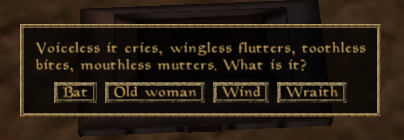
\includegraphics{media/image3.png}

Clicking on those buttons will just close the messagebox for the moment, and clicking on the chest again, nothing should happen either -- which is good, it means our do-once condition works.

\textbf{Ok, leave Morrowind and go back to the editor, and load your plugin again.}

We now need to figure out which answer the player selects, and script appropriate reactions for right and wrong answers. The function to test the selected answer is "GetButtonPressed". This function returns a number depending on which of the buttons of a message box has been clicked on with the mouse. It will return "0" for the first button ("bat" in our example) and 1, 2, 3 etc. for the following buttons, in the order you listed them in the messagebox function. While no answer
has been selected, the function will return --1, so we have to take care of that, too.

The "Activate" function will make our chest open, in fact activate will simply trigger the standard action that would usually be performed when you "use" the selected object -- e.g. doors would swing open, NPCs would initiate dialogue etc.

The following update to our script also demonstrates how you can use a control variable to force MW to process functions one after the other, although the complete script is processed every frame of the game: simply increment the control variable and test it in a series of if -- elseif statements. This is a very safe way of scripting for MW -- it may not always be necessary, but it's safe.

Please edit the script to the following:

\lstinputlisting{scripts/my_first_script03.txt}

Take a look at the part that starts with "\emph{if (controlvar == 1)}". We have set controlvar to 1 as soon as the chest got activated. Now we test for which button is being pressed. We do this by assigning the new variable "\emph{button}" a value returned by \emph{GetButtonPressed}. Since the script is still running, even while the game seemingly pauses to await your decision, we first test if no button has been selected yet -- return tells the game engine to stop processing the script for this frame.

Our correct answer was "wind" which corresponds to button number two -- if button number two gets pressed, we will tell the player that he gave the right answer, and "activate" will open the chests inventory in the usual way.

All other values of button mean that the player has selected a wrong answer, so we can use the "\emph{else}" command here. In this case we tell the player what a fool he was and the chest is not activated.

Now look at the little addition at the top of the script:

% Excerpt from external script. my_first_script03 [firstline=6, lastline=13]

\begin{lstlisting}
	If ( OnActivate == 1 )
	
	If ( controlvar == 0)
	
	MessageBox "Voiceless it cries, wingless flutters, toothless bites,
	mouthless mutters. What is it?", "Bat", "Old woman", "Wind", "Wraith"
	
	Set controlvar to 1
	
	elseif controlvar > 1
	
	activate
	
	endif
	
	endif
\end{lstlisting}

This means that, whenever the chest is activated in the future, it will only open if controlvar is greater than 1. Check above: when the player provides the wrong answer in the riddle, controlvar is set to --1, so he will never be able to open the chest. But if he knew the right answer, \emph{controlvar} is set to 2, and from now on the player can open the chest as often as he likes. Save and run your plugin, and test as described above.

\hypertarget{your-first-bug}{%
\subsubsection{Your first bug}\label{your-first-bug}}

Now, you will probably have noticed that the script does almost -- but not quite -- what we wanted. After clicking the correct answer, the chests inventory doesn't open as intended. Now, the logic above seemed fine, so what is wrong? \textbf{Let's try the following (change the corresponding part of your script according to the fragment below):}

% Excerpt from external script. [firstline=, lastline=]

\begin{lstlisting}
	if (controlvar == 1)
	
	set button to GetButtonPressed
	
	if ( button == -1 )
	
	return
	
	elseif ( button == 2 )
	
	MessageBox "The answer was correct"
	
	set controlvar to 2
	
	else
	
	MessageBox "The answer was wrong"
	
	set controlvar to -1
	
	endif
	
	elseif ( controlvar == 2 )
	
	Activate
	
	endif
\end{lstlisting}

See how I moved the activate command to the section that tests for controlvar == 2? This provides a cleaner sequence of events, and as I mentioned above, this can be very important when scripting for Morrowind -- always try to avoid doing too many things at once! \textbf{Well, run and test it.}

Great, now the inventory opens as we wanted, but what is this? The cursor is real slow, and we can't close the inventory! Look above -- \emph{controlvar} was set to two, and remains there, we do not change it again -- therefore the game now gets continuous "\emph{Activate}" commands each time the script is processed (every frame)! That's why we can't close the inventory -- it gets reopened immediately. \textbf{So change the following part of the script:}

% Excerpt from external script. [firstline=, lastline=]

\begin{lstlisting}
	elseif ( controlvar == 2 )
	
	Activate
	
	Set controlvar to 3
	
	endif
\end{lstlisting}

\textbf{Test again}: now everything works the way we wanted. I hope I have not confused you with the above excursion into the process of debugging, but it is a very important thing to know about -- you will constantly have to rethink your scripts and try different ways of doing it to be successful.

What is still missing? The trap effect of course!

\hypertarget{putting-a-spell-on-the-player}{%
\subsubsection{Putting a spell on the player}\label{putting-a-spell-on-the-player}}

Our chest will put a curse on the player if he fails to answer the riddle.

First go to the spellmaking tab in the editor, right click and select "new". Give the spell the ID "Frost\_Curse", name it "Frost Curse" and make it type "curse" then give it a magnitude of e.g. 1-5. It should look like in the picture below.

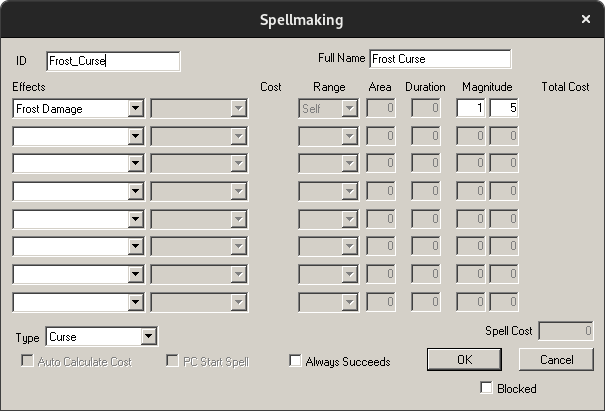
\includegraphics{media/frost-curse.png}

Now, we need to put this curse on the player. For this we use the \emph{AddSpell} function. After some time we will remove the curse again using the \emph{RemoveSpell} function, for this we need to make a timer. Edit your script again:

\lstinputlisting{scripts/my_first_script04.txt}

Let's go over this. Player-> AddSpell, "Frost\_Curse" puts the curse we created earlier on the player. Note how we need to use "Player->" to make sure the effect really targets the player. Otherwise we would curse the chest (which is the default object, because the script is attached to it), which wouldn't make a lot of sense\ldots{}

% Excerpt from external script. [firstline=, lastline=]

This bit:

\begin{lstlisting}
	Float timer
	
	Set timer to ( timer + GetSecondsPassed )
	
	if timer > 10
\end{lstlisting}

\ldots that is how you make a timer in Morrowind. \emph{GetSecondsPassed} is a function that returns the time in seconds that has passed since the last frame. Since this is usually a fraction of a second (as the script gets called every frame), it is only natural that we need a float variable for this purpose -- a variable that can store numbers with decimals. So when the timer has been running for 10 seconds we remove the curse again, and make sure we do this only once:

% Excerpt from external script. [firstline=, lastline=]

\begin{lstlisting}
	Player-> RemoveSpell, "Frost\_Curse"
	
	set controlvar to -2
\end{lstlisting}

Ok, save and test your mod. Works fine now, doesn't it? Well, almost. Try the following: let yourself be cursed, and then open your inventory. Wait. See how the curse terminates after some time, without hurting you? Of course: the script is still running, but spell effects are only calculated while in game, not while you are in the menu. We don't want the player to get off the hook so easily, so we need to put something in our script that stops it from processing when we are in menu mode. Luckily there is the \emph{MenuMode} function, which returns 1 when you enter the menu. So we can put this at the start of our script:

% Excerpt from external script. [firstline=, lastline=]

\begin{lstlisting}
	If ( MenuMode == 1 )
	
	Return
	
	Endif
\end{lstlisting}

Remember, return tells the game to stop processing the script for this frame.

Ok, now we have our final working script. Congratulations! If you want, experiment a little more with this script: Put the chest into a location in the game and lock it. Then try unlocking it (Unlock function) with the script in addition to activating it. Try adding a sound, when the riddle is successfully solved (e.g. PlaySound3D, "skillraise"). Try using the "Cast" function instead of "\emph{AddSpell}". Previous users of the Tutorial have spotted a potential bug in it: what happens if the player leaves the area with the scripted chest before the curse is removed again? How would you fix this?

This is the final script:

\lstinputlisting{scripts/my_first_script05.txt}

\hypertarget{how-to-learn-more}{%
\section{How to learn more}\label{how-to-learn-more}}

After this tutorial you may ask yourself how to continue with learning
how to script. A good way is to look at the example scripts in this
guide or at scripts that are already in the game (either form Bethesda
or from mods). Try to find a script that is similar to what you want to
do and then copy the script and change it to fit your needs. Read the
general information below and the descriptions of the functions you may
need to do what you have planned. The ordering of the functions into
thematic groups should help you to find the right ones.

Finally, the official forums are a great place to find information (use
the search function) or to get help on a specific problem. The rest is
practicing, practicing, practicing 
\includegraphics{media/image5.png}
\hypertarget{general-information-scripts-commands-and-syntax}{%
\section{\texorpdfstring{\hfill\break
General Information: Scripts, Commands and
Syntax}{ General Information: Scripts, Commands and Syntax}}\label{general-information-scripts-commands-and-syntax}}

\hypertarget{types-of-scripts}{%
\subsection{Types of scripts}\label{types-of-scripts}}

\hypertarget{local-scripts}{%
\subsubsection{Local scripts}\label{local-scripts}}

Any script that is running on an object or Actor in the game (assigned
in the script-dropdown field of the object or Actors object window) is a
local script. Local scripts are only active if the cell is loaded --
this is the current interior cell, or the current and all directly
neighboring exterior cells. When the object is outside of this range the
script is not running, but the local variables are saved. You cannot
stop a local script using Stopscript.

\hypertarget{global-scripts}{%
\subsubsection{Global scripts}\label{global-scripts}}

Any script that is not attached to any object is a global script, and is
by default not executed until you call it (see below). Note that there
is no default object for a global script to work on, so objects must
always be specified: while the following will work in a local script
attached to an NPC:

\begin{lstlisting}
	AITravel 1150, 8899, 1110
\end{lstlisting}

You will have to specify the NPC in a global script:

\begin{lstlisting}
	"NPC_ID"-> AITravel 1150, 8899, 1110 ;NPC_ID is the ID, the
	unique identifier for
	
	;each object in the editor
\end{lstlisting}

Global scripts are active all the time once they have been activated and
until they are specifically terminated. Thus, once activated, they will
be processed every frame as described for locals scripts above. That is
why they should be used with caution, as too many, or too complicated
global scripts can easily slow the game down a lot.

The command to start a non-active script is:

\begin{lstlisting}
	StartScript, "Script ID"
\end{lstlisting}

With Tribunal and Bloodmoon you also have the option to make a script
start automatically with the game. In the TESCS under the menu
Gameplay/Edit starting Scripts/ you can add any script to the list of
automatically started scripts.

The function to terminate a global script is:

\begin{lstlisting}
StopScript, "Script ID"
\end{lstlisting}

Variables local to a global script will be saved temporarily when the
script is stopped and restarted. In order to ensure that variables are
always saved, the script must be run at least once every load session.
If you need to be sure the variables are reset, you should reset them
yourself: don't rely on it happening automatically.

A simple way to ensure variables are saved is to use a startscript (only
available with expansions); so for example the startscript might look
something like this:

\lstinputlisting{scripts/KeepVarsScript.txt}

...and the script "MyScript" might look like this:

\lstinputlisting{scripts/MyScript.txt}

It is possible to use the StartScript function to run global scripts
that are tied to an object or Actor. These are called "targeted
scripts".

\begin{lstlisting}
	"Object_ID"-> StartScript "Script_ ID"
\end{lstlisting}

These scripts resemble both local scripts (in that the functions called
always default to the object or Actor the script targets) and global
scripts (in that they are always running and can be terminated with
StopScript).

\textbf{Note:} read more on the special case of "targeted scripts" in
the Tips and Tricks section.

\hypertarget{syntax}{%
\subsection{\texorpdfstring{\hfill\break
Syntax}{ Syntax}}\label{syntax}}

There are some unique features in TES script that should be explained
before we go into more detail.

\hypertarget{beginning-and-ending-scripts}{%
\subsubsection{Beginning and ending
scripts}\label{beginning-and-ending-scripts}}

\begin{lstlisting}
	Begin Script_ID
	
	End
	
	End Script_ID
\end{lstlisting}

Every script must have the Begin and End tags. The specified name will
also be the ID you will reference the script by (be it from other
scripts or inside the TES CS object windows). A script may start out
with comments, but the first line of real code must be "Begin
xxxxxxxxx".

As with other objects, it is recommended that you give your scripts a
unique tag. I usually use GBG\_Scriptname. This ensures that your
scripts are easily identified, they all are neatly listed in one block
in the scripts list, and there is little danger of conflicts with other
mods using the same name. Using leading underscores e.g. \_Scriptname is
not recommended.

If you want your scripts to appear at the top of the list of scripts,
put a 1 in front, for example, 1YAC\_ScriptName

\hypertarget{general-syntax-for-functions}{%
\subsubsection{\texorpdfstring{General syntax for functions:
}{General syntax for functions: }}\label{general-syntax-for-functions}}

Functions are not case sensitive, but using the case sensitive form as
suggested by Bethesda (e.g. GetSpellEffects instead of getspelleffects)
makes scripts easier to read, so it's recommended to keep it that way.

\begin{lstlisting}
	"Object_ID"-> Function, [parameters]
\end{lstlisting}

This is the format for all functions that act on or refer to a
specifiable object in the game world. The "arrow" or "fix" designates
which object a function will be performed on. The "object\_ID" is the
unique ID that is given to each object in the editor (usually the first
field in any object window). You need this ID, not the Name! If you call
a function without a designated Object-ID, the function will be
performed on the default object, which is the object the script is
attached to.

This is not to say that there might not be another object referenced as
a parameter:

\begin{lstlisting}
	"Object_ID1"-> Function, "Object_ID2"
\end{lstlisting}

\textbf{Notes:}

Functions with a "fix" will only compile if the object has already been
placed into the game world in the editor (with at least one reference),
otherwise the script will not compile. If you compile the script and
then delete all references, the game will give errors on load and CTD.

More than one function may be used in a \emph{set} expression, but the
functions always apply to the same reference. For example:

\begin{lstlisting}
	set SomeVar to ( player-> GetStrength ) + (
	player-> GetEndurance )
\end{lstlisting}

and

\begin{lstlisting}
	set SomeVar to ( player-> GetStrength ) + ( GetEndurance )
\end{lstlisting}

will both have the same effect, and specifying different references will
not work.

Referencing non-unique items with the "fix" will usually perform the
function only on the first reference of the object! So using this in a
global script:

\begin{lstlisting}
	"cliff racer"-> ModCurrentHealth -1000
\end{lstlisting}

will not have the desired effect, it will only kill one of the annoying
bastards. However attaching a script to the creature with just

\begin{lstlisting}
	ModCurrentHealth -1000
\end{lstlisting}

Would do the trick, because every reference of the cliff racer will have
the script running, and apply the function to itself. Note that this
does not apply to all functions (e.g. SetHealth in the above example
would affect all references the player has not yet encountered).

A number of functions refer only to the player or not to an object at
all, and are therefore using the fix is meaningless or may produce
errors. E.g.:

\begin{lstlisting}
	If ( GetPCRank == 0 )
	
	If ( CellChanged == 0 )
	
	FadeOut, 2
\end{lstlisting}

\hypertarget{general-syntax-commas-parentheses-and-spaces}{%
\subsubsection{General syntax: Commas, parentheses and
spaces}\label{general-syntax-commas-parentheses-and-spaces}}

TES Script is not too picky about syntax. Case mostly doesn't matter,
commas can be left out, and spaces are mostly ignored. Nevertheless I
would advise adhering to the following principles:

\begin{itemize}
\item
  Either avoid commas, or always use commas: inconsistent usage can
  cause problems.
\item
  If the ID contains a space or begins with an underscore, you must use
  quotation marks: "Object ID" or "\_Object\_ID". Better to avoid spaces
  altogether: Object\_ID
\item
  Get used to \textbf{always} leaving spaces around parentheses and
  operators, sometimes it seems to cause problems if you don't: if (
  variable == 1 ), not: if (variable==1).\\
  While this doesn't matter most of the time it generates weird and
  almost untraceable errors sometimes, so you are much better off always
  leaving a space.
\item
  The fix (->) is a little more complicated. If IDs are
  contained in quotes, you should \textbf{not} leave spaces around the
  fix:
\end{itemize}

\begin{quote}
"Sirollus Saccus"-> GetItemCount netch\_leather\_greaves
\end{quote}

The above will work, but spaces around the fix would cause problems.
(Thanks to Simpleton and DinkumThinkum for this info.) However, since it
has also been reported that a \emph{lack} of quotation marks can cause
problems in combination with spaces round the fix, I'm going to
recommend that you don't leave spaces round the fix at all (should be
fine in all cases).

\hypertarget{comments}{%
\subsubsection{Comments}\label{comments}}

Comments are marked by a semicolon ;. Comments can be added in their own
lines or behind lines with code.

\begin{lstlisting}
	\textbf{;} enter sneak mode
	
	Fargoth-> ForceSneak
	
	Fargoth-> AiTravel -11468.595,-71511.531,173.728
	\textbf{;}goes to tree
\end{lstlisting}

\hypertarget{indentation-using-tabstops}{%
\subsubsection{Indentation / using
tabstops}\label{indentation-using-tabstops}}

For your own sake, use proper indentation (tabstops) for if-elseif
constructs -- makes it much easier to keep track of them, so you don't
forget an endif at the end.

% In the tips and tricks section you will find a link to an external EMACS editor mode for TES script that will do automatic indentation.

\begin{lstlisting}
	If ( variable1 )
	
	If ( variable2 )
	
	{[}do something{]}
	
	endif
	
	endif
\end{lstlisting}
	
is better than

\begin{lstlisting}
	If ( variable1 )
	
	If ( variable2 )
	
	{[}do something{]}
	
	endif
	
	endif
\end{lstlisting}

\hypertarget{variables}{%
\subsection{Variables}\label{variables}}

\hypertarget{types-of-variables}{%
\subsubsection{Types of variables}\label{types-of-variables}}

There are three types of variables in the TES script language: short,
long and float. According to the manual these cover the following data
ranges:

	Short -32,768 to 32,767 (signed integer)
	
	Long -2,147,483,648 to 2,147,483,647 ( long signed integer)
	
	Float 3.4E +/- 38 (float, 7 digits)

Apparently the boundaries for Long given here are only partly correct,
in the TES-CS you can assign a maximum value of 2147483520 (Forum info /
Argent).

Theoretically there should be string variables too, but to my knowledge
these are not implemented. Unfortunately there are also no data types to
store Object\_Id's, which limits the power of the scripting language to
a certain extent.

Variables can be grouped into \emph{local} variables (valid only in the
script that declares them) and \emph{global} variables (valid in every
script).

\textbf{Note}: A long global is effectively a float! In a script, local
to that script a long will have a full 32 bits of precision. But used as
a global, the number of bits of precision drops to 24, as when it exists
globally a long \emph{is} a float. Mental Elf discovered this when
attempting to use "bit packing" to get 32 flags into a global long
(forum info / mental elf).

\textbf{A Note about Floats:}

Floating point numbers in a computer are stored in a format similar to
that used for scientific or engineering notation. The number is rounded
off to a fixed number of significant digits, any leading or trailing
zeros are dropped, and an exponent is added to indicate the correct
location of the decimal or binary point.

The number 2385901045 would be stored similar to this:

2.385901x10\textsuperscript{9}

In fitting the number into a fixed number of bytes, we have lost the end
3 digits, so the number is no longer quite what you set it to.

If you set a float to a small number, like 5.5, it would still be stored
as 5.5, because as it doesn't take up much room, no numbers need to be
cut off.\\
\strut \\
The advantage of this format is that a wide range of values can be
expressed using a relatively small number of digits or bytes. The
disadvantage is that the rounding off means floating point numbers don't
have the precision of an integer, so they shouldn't be used when you
need to make exact comparisons or keep track of exact counts.\\
\strut \\
For example, a floating point variable is fine if you just need to check
if a distance is greater or less than a certain value. But if you need
to check if the player has specific number of some item in their
inventory, then you want to use a long or short integer variable for the
count.

(Forum info / DinkumThinkum)

An example by BungaDunga shows that when doing math with floats, the
answer isn't always what you expect:

\begin{lstlisting}
	\textbf{Float num1}
	
	\textbf{Float num2}
	
	\textbf{Float num3}
	
	\textbf{Set num1 to ( 1 / 3 )}
	
	\textbf{;num1 is now 0.3333333}
	
	\textbf{Set num2 to 3}
	
	\textbf{;num2 is now 3\\
		\strut \\
		set num3 to num1 * num2}
	
	\textbf{;num3 is now 0.9999999, rather than what you would expect, 1.\\
		\strut \\
		if ( num3 == 1 )\\
		; Never happens.\\
		endif}
\end{lstlisting}

A lot of functions return float values (e.g. GetDistance, GetScale,
GetSecondsPassed\ldots): the same thing applies. Test a range, not an
exact value! E.g.:

\begin{lstlisting}
	if ( ( GetPos x ) == 500 )
	
	;will be false if it's 499.9999, or 500.0001, etc
	
	endif
\end{lstlisting}
	
but this will work:

\begin{lstlisting}	
	if ( ( GetPos x ) > 499.5 )
	
	if ( ( GetPos x ) < 500.5 )
	
	;it's close enough for me
	
	endif
	
	endif
\end{lstlisting}

\protect\hypertarget{_Toc182634499}{}{}

Another common mistake is to check if the GameHour is an exact number.
As the Gamehour variable is increased every frame, and every frame is a
slightly diffrent length, the Gamehour variable soon ends up with a
value like this, 10.12853. So never test if the gamehour is exatly equal
to a value, as it is very unlikley to happen, test if it is greater than
or equal to a value.

\hypertarget{local-variables}{%
\subsubsection{Local variables}\label{local-variables}}

Local variables these have to be declared in the script:

	Float floatvarname
	
	Short shortvarname
	
	Long longvarname

Local variables are unique to a specific instance of a local script.
This means that the local variables in multiple objects with the same
script do not influence each other. The names you use for variables are
pretty much up to you as long as they start with a letter, but you have
to avoid using function names (this will result in errors during
runtime) and reserved characters (e.g. - + / * = " )( etc.) which will
result in compiler errors. E.g. "variable-1" will not work as a variable
name. Underscores as in "my\_variable" are ok, but avoid leading
underscores. A dot has a reserved meaning as well (see
"\emph{Referencing variables in other local scripts}" below).

\hypertarget{global-variables}{%
\subsubsection{Global variables}\label{global-variables}}

To declare a global variable go to the Gameplay menu and select Globals.
Right click for "new", name it, and set the type and starting value for
the new global variable, if one is needed. By default it will be 0.
Global variables are very useful for involved quests when you need to
keep track of things over an extended time and space. They are also a
simple way to share information between different scripts

\textbf{Note}: if you declare a local variable with the same name as a
global variable, the global variable will become invisible for this
script. Do NOT declare a global variable as a local!

\hypertarget{referencing-variables-on-other-objects-and-scripts}{%
\subsubsection{Referencing variables on other objects and
scripts}\label{referencing-variables-on-other-objects-and-scripts}}

Set \ldots{} to

If a unique object has a local script running on it you can change
variables from outside the script in the following way:

\begin{lstlisting}
	Set MyObject.variable to 100
\end{lstlisting}

or

\begin{lstlisting}
	Set MyObject.variable to local_variable
\end{lstlisting}

This method changes a local variable in the object's script. The object
must have a script on it for this to be valid. The object does not have
to be in an active cell when setting the variable, but it will only work
if the cell containing the target object/(script) has previously loaded
-(Cyran0). \textbf{Note:} The scripting system looks at the first object
in the database, thus you should only reference objects that are unique
(exist only once).

Note that the reverse does \textbf{not} work:

\begin{lstlisting}
	Set local_variable to MyObject.variable ;this doesn't work!
\end{lstlisting}

Use a global variable to transfer information in this way, or set
local\_variable from the \textbf{other} script using the syntax above.

\begin{lstlisting}
	if ( anotherobject.x > 0 )
\end{lstlisting}

apparently works.

Furthermore I realized only recently that this syntax also works for
global scripts:\\
\strut \\

\begin{lstlisting}
	set Global_script_name.variable to 1
\end{lstlisting}

\strut \\
This is useful to avoid using more global variables then necessary or
also as a console command to debug global scripts.

\textbf{Note:} If your object or global script starts with a number, you
need to put quotes around it.

\begin{lstlisting}
	"11NPC01".RemoteVar ;-\/-\/-Good\\
	"11NPC01.RemoteVar" ;-\/-\/-BAD
	
	11NPC01.RemoteVar ;-\/-\/-BAD
\end{lstlisting}

A caution when setting variables from outside the script
(DinkumThinkum):

\emph{If you recompile the target script (i.e., the local script on
'MyObject'), it's a good idea to also recompile any scripts that
reference variables in that script. Reason: if the target 'variable'
winds up in a different position in the target script's list of
variables, then any scripts trying to set that variable will break if
they're not recompiled.}

I.e., if 'variable' is the 14th variable declared in the local script on
'MyObject', and you add a new variable ahead of it so that 'variable' is
now the 15th variable declared, other scripts will need to be recompiled
in order to find 'variable' in its new position, otherwise the script
will end up changing the wrong variable, leading to very strange bugs.

\emph{One way to reduce the chances of this tripping you up is declare
variables referenced by other scripts first,} before \emph{other
variables that aren't referenced externally. Then just be careful to
only add or remove variables} after \emph{the block of externally
referenced variables. However (to be safe), it's still a good idea to
recompile scripts that reference variables in other scripts any time
you've added or removed variables in the other scripts.}

\hypertarget{using-variables-in-functions}{%
\subsubsection{Using variables in
functions}\label{using-variables-in-functions}}

Unfortunately it is one of the limitations of TES script that only
certain functions accept variables as parameters, which poses some
definite limits. The type of arguments functions accept is indicated in
the list of functions below.

\textbf{Note:} For some functions where both a Get-Function and a
Set-Function exist, a workaround can be constructed by using the while
function (see below).

\hypertarget{section}{%
\subsubsection{}\label{section}}

\hypertarget{operators-mathematical-calculations}{%
\subsubsection{\texorpdfstring{Operators / mathematical calculations
}{Operators / mathematical calculations }}\label{operators-mathematical-calculations}}

You can use the standard operators to do calculations in scripts:

\begin{longtable}[]{@{}
  >{\raggedright\arraybackslash}p{(\columnwidth - 2\tabcolsep) * \real{0.82}}
  >{\raggedright\arraybackslash}p{(\columnwidth - 2\tabcolsep) * \real{0.18}}@{}}
\toprule
\begin{minipage}[b]{\linewidth}\raggedright
Addition:
\end{minipage} & \begin{minipage}[b]{\linewidth}\raggedright
+
\end{minipage} \\
\midrule
\endhead
Subtraction: & - \\
Multiplication: & * \\
Division: & / \\
\bottomrule
\end{longtable}

The syntax is as follows:

Set result\_var to (var\_a + var\_b)

Instead of variables, literal values are also allowed. I assume that
standard operator precedence applies ( * and / are calculated before +/-
). Since it has not been properly tested I usually always use
parentheses to be on the safe side. You can use parentheses according to
standard mathematical rules:

\begin{lstlisting}
	set ln to ( ln + ( k10 * math_ln10 ) + ( k2 * math_ln2 ) )
\end{lstlisting}

A warning: There are different opinions on the forums on the use of
several operators in one line. Some people report a lot of problems with
this, I myself have successfully used at least four operators and
variables in a single line. There appears to be an issue with very long
additions (e.g. adding up more than 20 variables in one line of code)
that causes a mod to crash the game upon loading. If this happens, split
the calculations to several lines.

\hypertarget{notes-by-dinkumthinkum}{%
\subparagraph{Notes by DinkumThinkum:}\label{notes-by-dinkumthinkum}}

\hypertarget{eleven-variables-in-a-single-set-statement-will-cause-the-following-error-when-loading-the-game-followed-by-a-crash-to-desktop}{%
\subparagraph{\texorpdfstring{\emph{Eleven variables in a single set
statement will cause the following error when loading the game, followed
by a crash to
desktop:}}{Eleven variables in a single set statement will cause the following error when loading the game, followed by a crash to desktop:}}\label{eleven-variables-in-a-single-set-statement-will-cause-the-following-error-when-loading-the-game-followed-by-a-crash-to-desktop}}

\hypertarget{need-more-room-for-zero-pointers-in-scriptreplaceglobalsindata}{%
\subparagraph{"Need more room for zero pointers in
Script::ReplaceGlobalsInData"}\label{need-more-room-for-zero-pointers-in-scriptreplaceglobalsindata}}

as soon as you click the button to acknowledge the error, CTD. (That
script name wasn't any script of mine; it's something internal to the
game.)

Six variables in a Set statement work fine. Don't know the maximum
number, but it's obviously at least six and definitely less than eleven.

There isn't much in the way of dedicated mathematical functions in TES
script. There is the 'Random' function and Tribunal added the
'GetSquareRoot' function (see below). If you need more complex
functions, I suggest downloading Soralis' Math Mod (available from
Planet Elder Scrolls). It's a collection of scripts that allow you to do
complex calculations. Here is a short excerpt from the readme to give
you an idea:

\emph{"This mod adds the ability to use various math functions within
Morrowind's scripts.}

Specifically, these are the scripts that are added:"

\begin{longtable}[]{@{}
  >{\raggedright\arraybackslash}p{(\columnwidth - 8\tabcolsep) * \real{0.20}}
  >{\raggedright\arraybackslash}p{(\columnwidth - 8\tabcolsep) * \real{0.15}}
  >{\raggedright\arraybackslash}p{(\columnwidth - 8\tabcolsep) * \real{0.22}}
  >{\raggedright\arraybackslash}p{(\columnwidth - 8\tabcolsep) * \real{0.32}}
  >{\raggedright\arraybackslash}p{(\columnwidth - 8\tabcolsep) * \real{0.12}}@{}}
\toprule
\endhead
Name & Check/Done & Inputs & Outputs & Accuracy \\
MathScripts & N/A & N/A & N/A & N/A \\
MathConstants & N/A & N/A & N/A & N/A \\
SquareRoot & 1 & math\_sqrt & math\_result, math\_imag & 7 \\
SineScript & 2 & math\_angle & math\_sin, math\_cos, math\_tan & 7 \\
ArcsineScript & 3 & math\_arc & math\_sin, math\_cos & 6-7 \\
NaturalLog & 4 & math\_log & math\_result, math\_imag & 4-5 \\
LogScript & 5 & math\_log, math\_base & math\_result, math\_imag &
3-4 \\
intPower & 6 & math\_value, math\_power & math\_result & 7 \\
intRoot & 7 & math\_value, math\_root & math\_result, math\_imag &
6-7 \\
Modulus & 8 & math\_value, math\_mod & math\_result & 6-7 \\
Antiln & 9 & math\_log & math\_result & 4-5 \\
Antilog & 10 & math\_log, math\_base & math\_result & 2-3 \\
AbsoluteValue & 11* & math\_abs & math\_abs & 7 \\
PowerScript & 12 & math\_value, math\_power & math\_result, math\_imag &
2-3 \\
\bottomrule
\end{longtable}

Unfortunately many of these functions are rather slow, and not suited
for real time calculations. For sine and cosine in particular, check out
JDGBOLT's script in the tips and tricks section, which uses
pre-calculated values for a very rapid calculation. You can also find
more information on UESP Wiki.

MWSE (Morrowind Script Extender) also adds trig functions to Morrowind.

\protect\hypertarget{_Toc182634504}{}{}

\hypertarget{testing-conditions}{%
\subsection{Testing conditions}\label{testing-conditions}}

\hypertarget{use-of-if-elseif-conditions}{%
\subsubsection{Use of if\ldots{} elseif
conditions}\label{use-of-if-elseif-conditions}}

	If (condition)
	
	Elseif (condition)
	
	Else
	
	Endif

Much of TES scripting relies on the use of \emph{if\ldots{} elseif}
conditions and variations thereof. It is very important to fully
understand these, and the conditions that can be used in them to test
conditions of the game world to trigger events.

In general a condition is "true" when it has the value of 1 (or simply
"not 0" (e.g. -1 is "true" in TES Script too) and "false" when the value
is 0. There are thus certain functions in the game that return "true"
under certain conditions. For example see the GetAIPackageDone function
further down. It returns "true" (= 1) for one frame when an AIPackage
has finished. All lines of code between the if-statement and endif
(which concludes a so-called "if block") will be executed only when the
condition is true.

Thus:

\begin{lstlisting}
	\textbf{If} ( GetAIPackageDone )
	
	;{[}do something here{]}
	
	\textbf{endif}
\end{lstlisting}

will be only executed when the GetAIPackageDone function currently
returns the value 1.

In addition to just a value, a condition can also be a more explicit
test of conditions. The conditions, such as "A equals B" or "A is
greater than B" will be evaluated, and the whole expression will be true
(equals 1) when the condition is fulfilled. E.g.:

\begin{lstlisting}
	\textbf{if} ( GetAIPackageDone == 1 )
	
	;{[}do something here{]}
	
	\textbf{endif}
\end{lstlisting}

Is equivalent to the example above. This second syntax tests a condition
and returns "true" if the condition is met. You can check for the
following conditions:

\begin{longtable}[]{@{}
  >{\raggedright\arraybackslash}p{(\columnwidth - 2\tabcolsep) * \real{0.54}}
  >{\raggedright\arraybackslash}p{(\columnwidth - 2\tabcolsep) * \real{0.46}}@{}}
\toprule
\endhead
\textbf{Verbose} & \textbf{Conditional operator} \\
"Equal to": & == \\
"not equal to" & != \\
"Greater than" & > \\
"Smaller than" & < \\
"Greater than or equal to" & >= \\
"Smaller than or equal to" & <= \\
\bottomrule
\end{longtable}

If you have several independent if blocks each will be evaluated
separately. If, e.g. the following if blocks are in your script:

\begin{lstlisting}
	if ( timer >= 2 )
	
	;{[}Block A,do something here{]}
	
	endif
	
	if ( timer <= 3 )
	
	;{[}Block B, do something else here{]}
	
	endif
\end{lstlisting}

Both will be true and the code in the blocks will be executed when timer
is between 2 and 3.

You can nest if-blocks if you want to make sure that two conditions are
fulfilled simultaneously:

\begin{lstlisting}
	if ( timer >= 2 )
	
	if ( controlvar == 0
	
	;{[}do something here{]}
	
	endif
	
	endif
\end{lstlisting}

The code in the inner if block will only be executed when both
conditions (timer >= 2 and controlvar == 0 ) are fulfilled at
the same time.

For more elaborate constructions you can use Else and Elseif. Elseif
tests for a separate condition if the preceding condition has failed
(but not if the previous condition was fulfilled)

\begin{lstlisting}
	if ( timer >= 2 )
	
	;{[}Block A,do something here{]}
	
	elseif ( timer <= 3 )
	
	; {[}Block B, do something else here{]}
	
	endif
\end{lstlisting}

unlike the example above, both blocks can not be true at the same time
now. Either timer is >= 2, then block A gets executed, or
timer is not >= 2 but <= 3, meaning effectively timer
is < 2, then block B gets executed. In all other cases,
neither block will be executed. You can have several elseifs behind each
other:

\begin{lstlisting}
	if ( counter == 1 )
	
	;{[}Block A,do something here{]}
	
	elseif ( counter == 2 )
	
	; {[}Block B, do something else here{]}
	
	elseif ( counter == 3 )
	
	; {[}Block C, do something else here{]}
	
	endif
\end{lstlisting}

An else creates a "default condition". The code following else will be
executed if all previously tested conditions are false:

\begin{lstlisting}
	\textbf{If} ( foo_var == 1 )
	
	[Block A: do something]
	
	\textbf{elseif} ( foo_var == 2 )
	
	[Block B: do something else]
	
	\textbf{else}
	
	[Block C: do something completely different]
	
	\textbf{endif}
\end{lstlisting}

In this example Block C will be executed it foo\_var is neither 1 nor 2.

\hypertarget{notes-and-cautions}{%
\subparagraph{Notes and cautions:}\label{notes-and-cautions}}

In my experience it is safest to use \emph{elseif} instead of multiple
separate \emph{if} statements if you test different states of one
variable.

Be careful using a function in a conditional ('If' statement); simple
functions seem to be OK, but ones with numeric parameters don't seem to
be reliable.

For example:\\
"If ( NewType != OldType )" worked correctly, but "If ( (
Player-> GetArmorType 0 ) != OldType )" always registered as
'Not equal', even if the variable 'OldType' had the same value as the
armor type that should have been returned by 'Get ArmorType 0'
function.\\
So use "Set NewType to ( Player-> GetArmorType 0 )", followed
by a separate 'If' statement to compare 'NewType' to 'OldType'.
-(DinkumThinkum)

\hypertarget{while-conditions}{%
\subsubsection{While conditions}\label{while-conditions}}

	While ( condition )
	
	; things to do
	
	EndWhile

The while command differs from the if command in that it is repeated
within one frame until the condition is fulfilled. This is best
explained with an example:

\begin{lstlisting}
	Short desiredAmnt
	
	SetStrength 0
	
	\textbf{while}( GetStrength < desiredAmnt ) ; non-literal
	value to match
	
	modStrength 1
	
	\textbf{endwhile}
\end{lstlisting}

This will set strength to the value in variable desiredAmnt after one
frame. The following script however would need an undetermined amount of
frames to do this, because the if condition is only called once each
frame:

\begin{lstlisting}
	if(getStrength < desiredAmnt) ; non-literal value to match
	
	modStrength 1
	
	endif
\end{lstlisting}

On the other hand the first example can potentially cause "freezing" (if
the value would be very high) while the second won't.

Note that this is a workaround for some functions to the problem of
functions not accepting non-literal values (variables) as arguments.

\hypertarget{constructing-boolean-operations-in-tes-script}{%
\subsubsection{Constructing Boolean operations in TES
Script}\label{constructing-boolean-operations-in-tes-script}}

Unfortunately there are no Boolean operators (AND, OR, NOT, XOR, \ldots)
in the scripting language. Thus you need to construct these yourself
using if\ldots{} elseif structures.

Instead of AND:

\begin{lstlisting}
	if ( variable1 AND variable2 ); does \textbf{not} exist
	
	{[}do something{]}
	
	endif
\end{lstlisting}
	
you have to use:

\begin{lstlisting}	
	If ( variable1 )
	
	If ( variable2 )
	
	{[}do something{]}
	
	endif
	
	endif
\end{lstlisting}
	
For OR constructs:

\begin{lstlisting}	
	if ( variable1 OR variable2 )
	
	{[}do this{]}
	
	endif
\end{lstlisting}
	
you can use elseif constructions:

\begin{lstlisting}	
	If ( variable1 )
	
	{[}do this{]}
	
	elseif ( variable2 )
	
	{[}do this{]}
	
	endif
\end{lstlisting}
% Chapter sectioning
%\protect\hypertarget{_Toc53412583}{}{}
\section{List of TES-script functions}

\hypertarget{explanation-of-the-format}{%
\subsubsection{Explanation of the
format}\label{explanation-of-the-format}}

First I will list the function and the arguments it takes:

{[}no fix{]} Code "string", arg\_enum, arg\_float, {[}optional{]}
(returns short)

{[}no fix{]} Indicates this function can never be used with a "fix"
meaning it can not be called by a specified actor. Functions without
this tag can be called by an actor, an object, or both.

Code: Name of the function

Arguments of the function: "string" indicates a literal string, such as
an object ID. arg\_enum indicates a literal value (no variables taken)
var\_float indicates a variable of the specified type (in this case
float). Brackets {[}{]} indicate optional parameters. (returns short) or
(returns float) indicate that the function returns a value and of what
type the value is. I will use the designation (returns Boolean/short) to
indicate a function that returns either 1 or 0 (a Boolean variable
although the game strictly speaking still uses a float)

Examples of usage follow in italics and are indented:

\emph{Code "ID", var\_enum, var\_float}

Example scripts are set in frames:

Begin script

{[}Script functions{]}

End script

From the 8\textsuperscript{th} edition onward the functions added with
Tribunal and Bloodmoon have been moved into the suitable sections of the
reference section. They are now marked with:

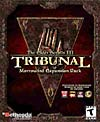
\includegraphics{media/image6.png} for Tribunal functions and

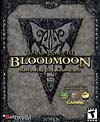
\includegraphics{media/image7.png} for Bloodmoon functions.

To use these functions the respective expansion must be installed (but
not necessarily active). Bloodmoon (and GOTY edition) incorporates all
functions from Tribunal as well.

\hypertarget{working-with-objects}{%
\section{\texorpdfstring{\hfill\break
Working with
objects}{ Working with objects}}\label{working-with-objects}}

\hypertarget{working-with-inventory-items}{%
\subsection{Working with inventory
items}\label{working-with-inventory-items}}

\hypertarget{adding-and-removing-items-from-the-inventory}{%
\subsubsection{Adding and removing items from the
inventory}\label{adding-and-removing-items-from-the-inventory}}

AddItem, "ObjectID", count\_enum

RemoveItem, "ObjectID", count\_enum

Actor-\textgreater AddItem, "item\_ID", 1

Container-\textgreater RemoveItem, "itme\_ID", 5

These functions are simple enough, adding or removing items from the
player's or any other inventory, including containers. A
\emph{RemoveItem} call will remove the item from the inventory, it will
"vanish".

\hypertarget{notes-on-additem-by-dinkumthinkum}{%
\subparagraph{Notes on AddItem (by
DinkumThinkum):}\label{notes-on-additem-by-dinkumthinkum}}

If you add items to an NPC's inventory when the inventory screen is
already open, the display won't be updated with the new items, unless
the player manually adds or removes displayed items (which forces the
game to refresh the inventory display).

The early versions of my Potion Saver coded used 'If MenuMode == 1' to
trigger putting potions back into the companion's inventory. This worked
fine when the companion was alive and conscious, since the script would
add the potions while in the dialogue window, \emph{before} the
companion share inventory window was opened.

However, if the companion was dead or unconscious, clicking on the
companion would open the inventory window immediately, and the potions
would be added after the window was already open. End result, the
potions wouldn't show up in the inventory window.\\
\strut \\
To avoid the problem, add items to an NPC's inventory as soon as they
die, as soon as they fall unconscious, or when the game goes into Menu
Mode (check Menu Mode \emph{after} checking death and unconsciousness).
That way, the items will be added before the inventory window opens.\\
\strut \\
Here's the code I used for this in the Potion Saver:

If ( GetHealth \textless{} 1 )\\
Set DTNPS\_HandlePotions to 0\\
ElseIf ( GetFatigue \textless{} 1 )\\
Set DTNPS\_HandlePotions to 0\\
ElseIf ( MenuMode == 1 )\\
Set DTNPS\_HandlePotions to 0\\
Else\\
Set DTNPS\_HandlePotions to 1\\
EndIf

\hypertarget{usage-with-containers}{%
\subparagraph{Usage with containers:}\label{usage-with-containers}}

If a container has been emptied by the player (in game), AddItem will no
longer work. One workaround is to replace the container with a new one
each time it's accessed by the player, but this may not be practical as
there's no way to detect when the container is empty. Aragon suggested a
solution:

The workaround is to attach a script to the container that always adds
and removes a dummy item in the same frame that the player activated it.
So, my ingredients chest has a script that looks like:

; Open the chest

Activate

; Always add and remove a dummy (this hack keeps the "AddItem" calls
working)

AddItem, "misc\_de\_cloth10", 1

RemoveItem, "misc\_de\_cloth10", 1

Furthermore, we make the chest with "references persist". Now we can
reference it from an ingredients sorter using code like:

set count to ( player-\textgreater GetItemCount,
"ingred\_dreugh\_wax\_01" )

while ( count \textgreater{} 0 )

set count to ( count - 1 )

player-\textgreater RemoveItem, "ingred\_dreugh\_wax\_01", 1

"\_tm\_ingredients\_chest"-\textgreater AddItem,
"ingred\_dreugh\_wax\_01", 1

endwhile

Another (probably better) workaround suggested by Enmesharra: Add a
non-carryable light with no world or inventory art associated with it to
the container. It won't show in inventory and thus the container can't
be emptied (not tested).

\hypertarget{notes-on-removeitem}{%
\subparagraph{Notes on RemoveItem:}\label{notes-on-removeitem}}

Removing items that are not present in the inventory does not crash the
game, but the 'RemoveItem' function will subtract the removed item's
weight from the character's encumbrance, EVEN IF the item is NOT in the
character's inventory. So if a script uses 'RemoveItem' to remove a 4
lb. item that the character doesn't have, the character's encumbrance
will wind up 4 lbs. lower than it should be. The workaround for this bug
is to always check for the presence of an item before using 'RemoveItem'
to delete it (Thanks DinkumThinkum for this info).

Don't remove an item that is executing a script, from the item's own
script: that will crash the game. See the example script.

A workaround for this is to use a separate global or local script to
remove the item. However, if the player has \textbf{two or more} copies
of an object with an attached script in their inventory, using
RemoveItem on that Object ID will frequently corrupt data for one of the
remaining copies (you may e.g. see corrupted health or count data).
Equipping or using that corrupt object may cause the game to crash
(Forum info / DinkumThinkum).

To avoid the two known RemoveItem bugs:\\
1. If the object is not scripted, use GetItemCount to be sure the player
has \emph{at least} 1.\\
2. If the object is scripted, use GetItemCount to be sure the player has
\emph{exactly} 1, or make sure the object is unique.

The drop function \emph{does not} have this bug. It does, however, cause
doubling, if used with OnPCEquip / SkipEquip, which can be fixed by
adding and removing any item as described for these functions.

\hypertarget{notes-on-using-additem-removeitem-in-dialogue}{%
\subparagraph{Notes on using Additem / Removeitem in
dialogue:}\label{notes-on-using-additem-removeitem-in-dialogue}}

\textbf{These functions can accept global variables, but only in
dialogue results}, and only if you don't set the global variable in the
same dialog result (Forum info / Argent; According to Argent, the
maximum amount he has been able to add using AddItem, var was 65534
(using a long var=2147483520)). In addition to Argent's info about
AddItem/RemoveItem accepting variables in dialog action boxes: make sure
that the variable in question doesn't change in the same box. Say,
var\_a equals 3 at the moment when the line is selected in dialogue. If
the result field looks like this:

set var\_a to var\_a + 10 ;

AddItem gold\_001, var\_a

three drakes will be added to NPC's inventory, and not thirteen. If such
need arises, put all calculating operators into one dialogue response's
result box, add "choice" operator, and process the AddItem function in
the following response. Also, even with long variables, I couldn't
correctly add values above 32767 (2\^{}15). (tested on pure Morrowind
without expansions) (Forum info / Kir).

Example script:

The following script was discussed on the forums (sorry don't remember
who first made it). It was supposed to ask the player if he wanted to
recycle an item when it was equipped, and then replace that item with
the "recycled" version.

\lstinputlisting{scripts/scr_thing.txt}

It worked nice enough without the \emph{RemoveItem} function in it, but
with that line it would crash. The reason was that this script was
\emph{attached} to item\_a, and thus the running script would be removed
with it, which apparently crashes the game. So the above idea had to be
handled via a global script.

\hypertarget{dropping-items-to-the-floor}{%
\subsubsection{Dropping items to the
floor}\label{dropping-items-to-the-floor}}

Drop, "ObjectID", count\_enum

"Actor\_ID"-\textgreater Drop, "ITEM\_ID", 1

This function is supposed to drop the item from the inventory "to the
calling Actor's feet". This seems to work correctly only for the player
character, dropping the item to his feet. When used on NPC's, the items
are removed correctly from the NPC, but still dropped at the player's
feet.

An interesting note on this is that if they really have that item, they
will drop it, with charges and condition intact. If they don't really
have that item, a new instance will be created. If the player drops an
item he doesn't have, his weight will still be reduced by the weight of
that item - same as the encumbrance bug for RemoveItem (Forum info /
DinkumThinkum).

Note that Drop will only work in active cells: if it is used on an NPC
in an inactive cell, nothing will happen. -(DinkumThinkum)

\textbf{Examples} of use are found in Bethesda's SlaveScript.

\hypertarget{monitoring-inventory-activities-adding-dropping-items-and-using-soul-gems}{%
\subsubsection{Monitoring inventory activities: Adding, dropping items
and using soul
gems}\label{monitoring-inventory-activities-adding-dropping-items-and-using-soul-gems}}

{[}no fix{]} OnPCAdd (is local short variable)

Short OnPCAdd

If ( OnPCAdd == 1 )

This variable is set to 1 when the PC added the object to inventory.
Must be reset manually for multiple use (set OnPCAdd to 0 ).

\textbf{Example:} This is an excerpt from the script attached to
Fargoth's ring, that gives you the magic menu during character creation:

if ( \textbf{OnPCAdd} == 1 ); Player has added the item to the inventory

if ( State == 0 )

EnableMagicMenu

MessageBox "You now have a Magic Menu, where you can see all your
powers, spells, and magic items." "Ok"

set state to 10

return

endif

endif

{[}no fix{]} OnPCDrop (is local short variable)

Short OnPCDrop

If ( OnPCDrop == 1 )

This variable gets set to one when the PC drops the object. Must be
reset manually for multiple use (set OnPCDrop to 0 ).

{[}no fix{]} OnPCSoulGemUse (is local short variable)

Short OnPCSoulGemUse

If (OnPCSoulGemUse == 1 )

This gets set to one if the calling Object is a soulgem and it has been
used in either recharging or item making. Must be reset manually for
multiple use (set OnPCSoulGemUse to 0 ).

Example: this is how Azura's star becomes an inexhaustible soulgem:

\lstinputlisting{scripts/AzurasStarScript.txt}

\hypertarget{force-equipping-an-item}{%
\subsubsection{\texorpdfstring{\hfill\break
Force-equipping an Item
}{ Force-equipping an Item }}\label{force-equipping-an-item}}

Equip, "Object\_ID" {[}count\_enum{]}

"Actor\_ID"-\textgreater Equip, "iron dagger"

(Also see OnPCEquip function below)

\textbf{Pre-Tribunal: Partly Broken.} This could have been an immensely
useful function. Unfortunately, most of the potential uses do not work:
You can NOT autoequip anything on the Player. You can NOT force the
Actors to equip weapons or armor with this (this is completely governed
by their skills with armor or weapons). You can NOT make "non-removable"
items, like cursed armor, etc. You CAN make Actors swallow potions, or
so I heard.

This Function was \textbf{fixed in Tribunal}. You can now force Actors
to equip armor, weapons and clothing. So you now CAN do all of the above
. Praise to Bethesda.

\textbf{Note}:

The Equip function can make someone equip an item they aren't carrying,
and it will add it to their inventory. However, if you do that then any
scripts on the items won't be run. So you need to use AddItem first,
then Equip, even though Equip does seem to add them. The script will
start if you take the item off the person or out of your inventory and
drop. But while it is in inventories the script doesn't start (Forum
info, ThePal).

In addition, it appears that Equip will only work on the player after at
least one AddItem has been used. -(DinkumThinkum)

The count is optional; if it's omitted then one item will be equipped.
You can't use this to force equip more than one item if it's not
possible to have more than one equipped at a time (e.g. a cuirass) - it
doesn't cause problems but it will still equip only one.

On using equip with variables: it didn't throw any errors, but I got
some strange results. It certainly didn't reliably equip the given
number.

\textbf{Note:\\
}If you equip a potion on a NPC, the NPC will not drink it. You could
get around this by making a spell with the same effects as the potion,
then removing the potion and adding the spell.\textbf{\hfill\break
}

\textbf{Sample Script:} This script (Tribunal required) curses an item
(a Chitin Club) so that it can't be unequipped anymore. Not even using
quick-keys. Bugger! Now you have to fight with a chitin club to the end
of your days, which will probably come soon The player can still use
magic however.

\lstinputlisting{scripts/cursed_item.txt}

\hypertarget{detecting-if-an-item-has-been-equipped}{%
\subsubsection{Detecting if an item has been
equipped}\label{detecting-if-an-item-has-been-equipped}}

{[}no fix{]} OnPCEquip (is local short variable)

Short OnPCEquip

If ( OnPCEquip == 1 )

The PC has the object equipped (remains true while object is equipped)

This game variable \textbf{(needs to be declared}!) gets set to 1 if the
player is equipping the calling object. It will remain "true" while the
item is still equipped, but gets reset to 0 if the item is unequipped.
So, in some cases you might want to manually reset it:

if ( \textbf{OnPCEquip} == 1 ) ; when the item is equipped

{[}do something{]}

set \textbf{OnPCEquip} to 0 ; do this once per equip event\ldots{}

endif

The next time the item is unequipped and equipped again, the functions
in {[}do something{]} will be performed again. You can also use a status
variable to control when an effect will be executed. Note that this can
also be processed while in Menu mode:

If ( MenuMode == 1 )

if ( \textbf{OnPCEquip} == 1 ) ; when the item is equipped

{[}do something{]}

set OnPCEquip to 0 ; do this once per equip event\ldots{}

endif

endif

This script will execute while you are in the menu, as soon as the item
is equipped, while the following will be executed only after you leave
the menu:

If ( MenuMode == 1 )

Return

Endif

if ( \textbf{OnPCEquip} == 1 ) ; when the item is equipped

{[}do something{]}

set \textbf{OnPCEquip} to 0 ; do this once per equip event\ldots{}

endif

An additional \textbf{Sample Script} can be found above with the Equip
function.

\textbf{Notes:} OnPCEquip was successfully tested with the following
item types:

Clothing

Armor

Weapons

Books/Scrolls (see tips and tricks for correct use, though)

Miscellaneous items

Usable lights

Probes

Potions and Ingredients will only register with OnPCEquip when you use
SkipEquip at the same time, otherwise the item is apparently "destroyed"
before the function registers! Repair objects suffer from this too, and
weirder still, apparatus (or alembics anyway) work the reverse way. They
only seem to trigger OnPCEquip when PCSkipEquip is NOT set (Forum info /
ManaUser).

Apparently books (and maybe some of the other item types that behave
strangely?) set SkipEquip to 1 instead of OnPcEquip! See the tips and
tricks section on this issue.

\hypertarget{disabling-ability-to-equip-an-item}{%
\subsubsection{Disabling ability to equip an
item}\label{disabling-ability-to-equip-an-item}}

{[}no fix{]} PCSkipEquip (is short variable)

Short PCSkipEquip

Set PcSkipEquip to 1

Set this to 1 to skip equipping object. Good for popping up messages for
breaking seals on books and such. For an extended example look at the
SealedTreasuryReport script in the editor. Its also great for using e.g.
clothing objects as script triggers in connection with the OnPCEquip
function (see my climbing mod for an example, the climbing gear is
actually a belt, but of course cannot be equipped).

\textbf{Note:} Apparently equipping a book in inventory sets this to one
(instead of setting OnPCEquip to one, as it should). See tips and tricks
section.

There is a bug associated with using this, that leads to duplication of
the item that has the SkipEquip function. I have seen this happen both
with QuickKey usage and when normally equipping items from the inventory
when OnPCEquip is also called. To bypass this, reset the inventory by
adding and removing a dummy item (from within the section of the script
that checks the OnPCEquip function). Do not remove the item with the
script itself, as this causes a crash (see RemoveItem function). If you
have a lot of SkipEquip items, make the item call a global script
(StartScript) that adds and removes the item, e.g.:

\lstinputlisting{scripts/doubling_fix.txt}

\textbf{Sample Script:} Here is a short script I made for a werewolf
mod, it makes an item non-equippable under certain conditions:

\lstinputlisting{scripts/non_equippable.txt}

\hypertarget{checking-for-presence-of-items-in-inventory}{%
\subsubsection{Checking for presence of items in
inventory}\label{checking-for-presence-of-items-in-inventory}}

GetItemCount, "ObjectID" (returns short)

Short objectcount

Set objectcount to ( "Mob\_ID"-\textgreater GetItemCount, "Object\_ID" )

If ( GetItemCount, "Object\_ID" \textgreater= 1 )

This function checks the inventory of the calling object and returns the
number of objects of type "Object\_ID" it owns.

\hypertarget{section-1}{%
\subsubsection{}\label{section-1}}

\hypertarget{repairing-objects}{%
\subsubsection{Repairing objects}\label{repairing-objects}}

{[}no fix{]} OnPCRepair (is short variable)

Short OnPCRepair

If ( OnPCRepair == 1 )

A game variable that gets set to 1 when the PC repairs the object with
the script. Requires manual reset.

RepairedOnMe, "Object ID" (returns Boolean/short)

if ( "daedric\_mace"-\textgreater RepairedOnMe, "repair\_journeyman\_01"
== 1 )

This function returns 1 if the calling item is repaired by an item of
type "Object ID". Object ID has to be of type "Repair Item" and the
calling object must be either weapon or Armor.

OnRepair

The similar function OnRepair is apparently broken. It should get set to
1 when any repair is attempted at the object: "returns true if calling
object is repaired at all".

\hypertarget{worn-equipped-object-information}{%
\subsubsection{Worn / equipped object
information}\label{worn-equipped-object-information}}

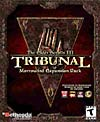
\includegraphics{media/image6.png}

GetWeaponType (returns short)

If ( Player-\textgreater GetWeaponType == 0 )

;Player uses a short blade

GetArmorType, armorPart\_enum (returns short, -1 to 2)

If ( Player-\textgreater GetArmorType, 0 == 2 )

;Player wears a heavy helmet

These functions are called on an Actor to gather information regarding
what the Actor has equipped. GetWeaponType returns the weapon type (see
Table 1.1) of the Actor's current weapon. GetArmorType returns the armor
weight (see Table 1.3) of the Actor's currently equipped armor part. The
armor parts are coded by the numbers listed below (see Table 1.2).
HasItemEquipped returns 1 if the Actor has the given item currently
equipped and 0 if it does not.

Note: If an NPC has a bow but no arrows and fights using hand-to-hand
(no other weapons), GetWeaponType 9 will still return true and
HasItemEquipped will return true for the bow.

\textbf{\hfill\break
Weapon types (Table 1.1):}

\begin{longtable}[]{@{}
  >{\raggedright\arraybackslash}p{(\columnwidth - 2\tabcolsep) * \real{0.61}}
  >{\raggedright\arraybackslash}p{(\columnwidth - 2\tabcolsep) * \real{0.39}}@{}}
\toprule
\endhead
\textbf{Weapon Type Name} & \textbf{Type Number} \\
Unarmed & -1 \\
Short blade, 1 hand & 0 \\
Long blade, 1 hand & 1 \\
Long blade, 2 hand close & 2 \\
Blunt, 1 hand & 3 \\
Blunt, 2 hand close & 4 \\
Blunt, 2 hand wide & 5 \\
Spear, 2 hand wide & 6 \\
Axe, 1 hand & 7 \\
Axe, 2 close & 8 \\
Bow & 9 \\
Crossbow & 10 \\
Thrown weapon & 11 \\
Arrow\textless?\textgreater{} & 12 \\
Bolt\textless?\textgreater{} & 13 \\
\bottomrule
\end{longtable}

\textbf{Armor parts (Table 1.2):}

\begin{longtable}[]{@{}
  >{\raggedright\arraybackslash}p{(\columnwidth - 2\tabcolsep) * \real{0.57}}
  >{\raggedright\arraybackslash}p{(\columnwidth - 2\tabcolsep) * \real{0.43}}@{}}
\toprule
\endhead
\textbf{Armor Part Name} & \textbf{Part Number} \\
Helmet & 0 \\
Cuirass & 1 \\
Left Pauldron & 2 \\
Right Pauldron & 3 \\
Greaves & 4 \\
Boots & 5 \\
Left Gauntlet & 6 \\
Right Gauntlet & 7 \\
Shield & 8 \\
Left Bracer & 9 \\
Right Bracer & 10 \\
& \\
\bottomrule
\end{longtable}

\textbf{Armor types / weight (Table 1.3):}

\begin{longtable}[]{@{}
  >{\raggedright\arraybackslash}p{(\columnwidth - 2\tabcolsep) * \real{0.57}}
  >{\raggedright\arraybackslash}p{(\columnwidth - 2\tabcolsep) * \real{0.43}}@{}}
\toprule
\endhead
\textbf{Armor Type Name} & \textbf{Type Number} \\
Unarmored & -1 \\
Light Armor & 0 \\
Medium Armor & 1 \\
Heavy Armor & 2 \\
\bottomrule
\end{longtable}

HasItemEquipped "item\_ID" (returns short)

If ( Player-\textgreater HasItemEquipped "chitin club" == 1 )

;you poor dolt!

\textbf{Sample Script:}

When this script is placed on an object, Activating a reference to that
object does ``damage'' to it based on the PC's current weapon and
strength. If the weapon is the specific weapon ``Rock Splitter'' the
object is fully damaged in one hit. When the object is fully damaged, it
explodes sending shards into the PC's face unless he has a shield or a
helmet equipped.

% Bug here? no end

\lstinputlisting{scripts/breakme.txt}

\hypertarget{usedonme-function}{%
\subsubsection{UsedOnMe function}\label{usedonme-function}}

UsedOnMe, ``Object ID'' (returns Boolean/short)

if ( UsedOnMe, Misc\_pot\_redware\_01 )

According to helpfile:

"Returns true if the ``Object ID'' has been used on the calling object.
This is used for scripts that make objects do certain things of the
player uses an object on it."

According to current knowledge this function is broken.

\hypertarget{moving-and-placing-objects}{%
\subsection{Moving and placing
objects}\label{moving-and-placing-objects}}

The following functions do not work on the player, NPCs or monsters.
They do work on static objects, activators, containers, miscellaneous
objects etc. \textbf{Note:} Actors, including the PC tend to fall
through moving objects after a while. This can be avoided by quickly
disabling and enabling a moving object every frame -- doing this
apparently updates the collision information. Actors can also be
equipped with a levitate or slowfall ability to further decrease the
chance of falling through objects (for more details see the tips and
tricks section on ridable objects by MadMax).

\hypertarget{moving-along-an-objects-axis}{%
\subsubsection{Moving along an objects
axis}\label{moving-along-an-objects-axis}}

Move axis(x/y/z), units/sec\_enum

Move x, 100

Object\_ID-\textgreater Move Z, 30

Moves the object along the selected axis (x, y, or z) at the speed
selected. This speed is in units per second (21.3 units per foot). Thus,
the distance moved per frame will depend on your frames per second,
while the distance moved in a unit time will not. This movement is based
on the object's local coordinate system. Thus, a positive y movement
will always move the object along its local forward vector:

\textbf{Note:} Move will not work on Actors, including the player.
However, it will work on dead actors (Forum info / Argent). As with all
functions using a "fix", move requires that the object is placed into
the game world in the editor, before you can use it in a script:

PlaceAtPC "My\_Object", 1,1,1

My\_Object-\textgreater Move x, 10

will not work if "My Object" has not already been placed, but you can
have a local script running on "MyObject" that just uses

Move x, 10

\hypertarget{moving-along-the-world-axis}{%
\subsubsection{Moving along the world
axis}\label{moving-along-the-world-axis}}

MoveWorld axis(x/y/z), units/sec\_enum

MoveWorld z, 100

Object\_ID-\textgreater MoveWorld Z, 30

Moves the object along the selected world axis (x, y, or z) at the speed
selected. This speed is in units per second (21.3 units per foot). This
movement is based on the world axis, thus a positive z movement will
always move the object up, regardless of its local rotation: In world
coordinates Z is always up / down (increasing upwards), X is east / west
(increasing to east) and Y is north / south (increasing to north).

\textbf{Note:} MoveWorld will not work on Actors, including the player.
Use SetPos for actors.

This is an \textbf{example} after a script I once picked up on the
forums that makes a platform slowly move out and back once the player
stands on it:

\lstinputlisting{scripts/platform_script.txt}

\hypertarget{cellupdate}{%
\subsubsection{CellUpdate}\label{cellupdate}}

CellUpdate

\textbf{Broken!} According to Bethesda: Updates the current object's
cell position. This should be called when moving objects over large
distances. The game keeps tracks of objects based on what cell they are
in, and if an object moves a cell over from its starting position, it
may not get processed correctly when running its script.

The part about not processing correctly is certainly right. Objects can
disappear or "warp" if moved too far from the place they were created
in. Unfortunately my attempts to use this function always resulted in a
runtime error: "need to add function code for function CellUpdate".

\textbf{Note:} a way around this problem (requires Tribunal) is to
disable and delete (SetDelete) the object on a regular basis (for
ridable objects upon entering a new cell) and immediately placing a new
version (PlaceItem) at the very same position using a global script
(seen in MadMax boat script from the Fishing Academy Mod). See the Tips
and Tricks section for an in-depth explanation by MadMax himself. This
works like a charm, because this way the object never really leaves the
cell it was created in.

\hypertarget{setting-position-the-other-way-to-do-movement}{%
\subsubsection{Setting position (the other way to do
movement)}\label{setting-position-the-other-way-to-do-movement}}

SetPos, axis, float\_enum\_pos (float\_var with Tribunal/Bloodmoon)

SetPos, z, 477

Object\_ID-\textgreater SetPos X, 466

This function (unlike the move and moveworld functions) also works with
Actors, including the player. Axis is x, y, or z. The float value sets
the position of the calling object to that value. This always refers to
the local coordinate system the object is currently in.

\textbf{Note:} With Tribunal, this function accepts local float
variables, but only within the currently active cells. This is relevant
for exteriors, you can not move objects an arbitrary distance, the
target location must be within the active cells (current cell of player
plus surrounding cells). (Forum info / reposted by Srikandi). Also note
that while objects can be SetPos to any position (without collision
being detected), Actors will still check for collision, and may not move
as expected in case of collision (which can be used to good effect for
collision detection).

\textbf{SampleScript:} This script is made for floating crates in the
Mournhold sewer (Tribunal). It demonstrates how \emph{SetPos} and
\emph{SetAngle} can be used instead of \emph{MoveWorld} and
\emph{Rotate} to produce fluid movements:

\lstinputlisting{scripts/floatAboveStartHeight.txt}

\hypertarget{positioning-an-object-in-the-world-or-in-an-interior-cell}{%
\subsubsection{Positioning an object in the world or in an interior
cell}\label{positioning-an-object-in-the-world-or-in-an-interior-cell}}

\textbf{Position, float\_enum\_x, float\_enum\_y, float\_enum\_z,
float\_enum\_zRot}

(for outdoors)(floats accepted with expansions)

\textbf{PositionCell, float\_enum\_x, float\_enum\_y, float\_enum\_z,
float\_enum\_zRot, ``cellID''\\
}(for interior / exterior cells) (floats accepted with expansions)

position -23515, -15355, 3355, 90

Player-\textgreater position -23515, -15355, 3355, 90

"Actor\_ID"-\textgreater PositionCell, -254, 475, -376, 360, "Balmora,
Council Club"

The classic application for this function is the teleport ring,
transporting the player to certain locations. However, it can also be
used to warp NPCs or objects to a new location. Note that in original
Morrowind this function only accepted literal values as arguments. (This
probably changed with Tribunal: not sure if in all versions or only with
the expansions, but: Position/PositionCell can take float variables, but
they must be LOCAL variables! (info by Indigo Rage).

Z\_Rot is not set in degrees (0-360°) but in minutes (1° = 60 min): So,
if you want the person to face east, use 5400. South, 10800. West 16200.

However, for some reason degrees are used for the player (thanks to Axel
for pointing this out).

\textbf{Notes:}

Using PositionCell in dialog results isn't reliable, and may cause
crashes: some users have no problems with it, but for others it will
crash the game, and for some users it may simply fail unpredictably
(this doesn't seem to be version-dependent, not sure what causes it).
The way Bethesda does this correctly is to use StartScript to start a
script that does the teleporting. (Forum Info/Emma).

You should not use this function on items that are in the players
inventory, this causes MW to crash (Forum info/Nigedo).

If you are repositioning the player immediately on detecting PC cell or
CellChanged (e.g. preventing teleport to a forbidden destination), you
may need to introduce a delay of one or two frames before using
PositionCell to move the player back out of the cell, otherwise the
player may not end up at the correct coordinates. (Forum info /
Monica21)

\textbf{Sample Script:} A simple teleport ring could look like this:

\lstinputlisting{scripts/TeleportScript.txt}

Note that both targets are outdoor cells and the different formats used.
If you try to teleport to an unsafe place (clipping with an object or
out in the void), you will instead be placed at the next safe location.

Sometimes the PositionCell format given above won't work (even though it
should): If there are no errors but nothing happens, try replacing, e.g.

Player-\textgreater PositionCell -21278, -17613, 534, 0, "Balmora (-3,
-3)"

with

Player-\textgreater PositionCell -21278, -17613, 534, 0, "Balmora"

I've found that sometimes one method works and sometimes the other.

\hypertarget{resetting-an-object-to-its-original-position}{%
\subsubsection{Resetting an object to its original
position}\label{resetting-an-object-to-its-original-position}}

SetAtStart

SetAtStart

Object\_ID-\textgreater SetAtStart

This resets the object to the original position it was given in the
editor, before any movement or rotation occurred. For an example, see
the moving platform script example under the topic "moving along the
world axis". See the \emph{Move} function for a sample script.

\hypertarget{placing-an-item-near-the-pc}{%
\subsubsection{Placing an item near the
PC}\label{placing-an-item-near-the-pc}}

{[}no fix{]} PlaceAtPC, "Object\_ID", count\_enum, distance\_enum,
direction\_enum

PlaceAtPC, "Secret Message", 0, 30, 1

PlaceAtPC, "ancestor\_ghost", 1, 256, 1

This function places a new reference of "Object\_ID" near the player.
The function lets you define a direction relative to the player where
the object is going to appear and a distance (in units). If that
location is not safe (in the air, in a wall, etc), the object will be
placed at one of the other axis or at the player's exact location
(feet). (Erratum: Thanks to Isildur and Esteban for pointing out that
number\_enum and distance\_enum were switched around in previous
versions.)

Direction is:

0 = front

1 = back

2 = left

3 = right

Note (DinkumThinkum):

\emph{According to Bethesda, on the PC version an overflow loot bag will
be created if there are more than 1024 objects in a single cell.}

\emph{\hfill\break
However, if you try to put a large number of objects into a cell using
'PlaceAtPC', the game will lockup completely. Don't know the minimum
number that will cause the crash, but 'PlaceAtPC p\_restore\_health\_e
2000 0 0' will definitely do it.}%☺

In other words: the game engine won't create an overflow loot bag for
excess items that are added to a cell by a script; instead, it just
crashes when the maximum number of items per cell is exceeded. I ran
into this with 'PlaceAtPC', but I would guess that any script function
that adds items to a cell would have the same problem. I would also
guess that the crash occurs as soon as the number of items in the cell
reaches the number that would normally trigger the creation of an
overflow loot bag.

\hypertarget{place-items-near-an-object}{%
\subsubsection{Place items near an
object}\label{place-items-near-an-object}}

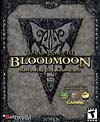
\includegraphics{media/image7.png}

PlaceAtMe "Item\_ID" count\_enum, distance\_enum, direction\_enum

Object-\textgreater PlaceAtMe `Item\_ID' count\_enum distance\_enum
direction\_enum

The PlaceAtMe function works the same as PlaceAtPC without it being
centered on the PC. Bloodmoon uses this to place attackers in different
places depending on the player's distance at the time. This allows the
script to make it appear as though there is a large number of opponents
that just keep coming, among other things.

;THIS POPS IN A HUNTER AT APPROPRIATE SPOT, INCREMENTS HUNTERCOUNT, AND
RESETS TIMER

if ( popA == 1 )

"active\_BM\_hunter1"-\textgreater{}\textbf{PlaceAtMe} skaal\_hunter 1 1
1

set huntercount to ( huntercount + 1 )

set timer to 0

elseif ( popB == 1 )

"active\_BM\_hunter2"-\textgreater{}\textbf{PlaceAtMe} skaal\_hunter 1 1
1

set huntercount to ( huntercount + 1 )

set timer to 0

elseif ( popC == 1 )

"active\_BM\_hunter3"-\textgreater{}\textbf{PlaceAtMe} skaal\_hunter 1 1
1

set huntercount to ( huntercount + 1 )

set timer to 0

endif

\hypertarget{creating-new-object-references-with-placeitem}{%
\subsubsection{Creating new object-references with
PlaceItem}\label{creating-new-object-references-with-placeitem}}

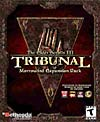
\includegraphics{media/image6.png}

{[}no fix{]} PlaceItem "object ID", float\_var\_X, float\_Y, float\_Z,
float\_Zrot

{[}no fix{]} PlaceItemCell "object ID", "cellID", X, Y, Z, Zrot

These functions are used to create new references to objects. PlaceItem
will create a reference to object "Object ID" at coordinate (X, Y, Z)
with Z rotation Zrot in the current cell. \textbf{Z\_Rot is not set in
degrees (0-360°) but in minutes (1° = 60 min): So, if you want the
person to face east, use 5400. South, 10800. West 16200.}

The function accepts (local) float variables. PlaceItemCell does the
same thing as PlaceItem except it allows you to specify a cell other
than the current one in which the object should be created. With either
function, if the target cell for the reference is an exterior cell and
the given coordinate is outside of that cell, then the reference will be
added to the cell containing the coordinate. This is a nice addition
that allows you to add things to the world without previously placing
them in the editor.

JOG posted the following interesting info on PlaceItemCell:

Well, When I first tried PlaceitemCell, I thought it's a great function
to place items instead of having a "storage-cell" where the objects lie
around until the game needs them. I soon realized that you can't refer
to those objects by script. (To disable them for example.) The script
won't compile until at least one of the objects is in use, and then the
disable command would refer to that object, so you still need
PositionCell.

(Note by GBG: you can circumvent this for many applications by having a
script on the placed item, so that you can omit the "fix" and have
functions such as disable reference to it by default.)

DinkumThinkum adds:

PlaceItemCell would have been perfect for what I wanted to do, until I
discovered that the placed NPC disappeared if I saved and reloaded
before going to the cell they were placed in.

(Note by GBG: This can be avoided in most cases by making the placing of
the NPC conditional on the player entering the cell. I still think
PlaceItem is a very useful function.)

Sample Script:

Putting this script on an object causes it, on activation, to ask the
user for an object type and then to create a reference to the specified
object at 100 units above the activated reference with 45 degree Z
rotation. If the key is selected, it is created at that same coordinate
and rotation in the cell ``key room'' rather than the current cell.

\lstinputlisting{scripts/makethingsimple.txt}

\hypertarget{rotation-and-angles}{%
\subsection{\texorpdfstring{Rotation and angles
}{Rotation and angles }}\label{rotation-and-angles}}

Bethesda uses both degrees and minutes (1° degree = 60 minutes) as units
in scripting functions:

GetAngle {[}°{]} (-180 to 180 °)\\
Setangle {[}°{]}\\
Position {[} min {]}\\
PositionCell {[}min{]} \emph{except for the player {[}°{]}}\\
PlaceItem {[}min{]}\\
PlaceItemCell {[}min{]}\\
Rotate {[} ° / second {]}\\
RotateWorld {[} ° / second {]}

\hypertarget{making-an-object-spin}{%
\subsubsection{Making an object spin}\label{making-an-object-spin}}

Similar to the movements described above, you can also rotate objects,
around either their local or the world axis and determine the current
angle:

Rotate , axis, angle/sec\_enum

RotateWorld, axis, angle/sec\_enum

Rotate, z, -30; rotate counterclockwise, 30° per second, around objects
z axis

Object\_ID-\textgreater Rotate, Y, 100

Axis can be x, y, or z. Notice that like the move functions the value
you are giving Rotate or RotateWorld is a speed setting (not an angle),
if you want to turn an object by 90\% either use set angle (for an
instantaneous change) or use Rotate together with GetAngle to check how
far the object has already been turned. These functions can not be used
with Actors.

RotateWorld does NOT update an item's position.\\
If you use RotateWorld in a script, and then call GetAngle, it will
always return the same value, regardless of what the angle actually is.
Just using rotate does not cause this problem.

(Forum info / HeyYou)

\hypertarget{setting-angles}{%
\subsubsection{\texorpdfstring{Setting Angles
}{Setting Angles }}\label{setting-angles}}

SetAngle, axis, float\_enum\_angle

SetAngle, z, 30

Object\_ID-\textgreater Setangle, z, 25

This function sets the object to a specific world angle. Axis is x, y,
or z. The float value sets the angle (in degrees) of the calling object
to that value. This always refers to the local coordinate system the
object is currently in.

\textbf{Note:} According to console test, this does not affect Actors.
With Tribunal, this function accepts local float variables, but only
within the currently active cells. This is relevant for exteriors, you
can not move objects an arbitrary distance, the target location must be
within the active cells (current cell of player plus surrounding cells).
(Forum info / reposted by Srikandi). For actors, see the "Face, x, y"
function.

Notes (by Simpleton):

SetAngle doesn't work how sfd says it does. My guess is nobody ever
noticed before because nobody ever uses it with the X or Y axis, which
is where it gets funky. I wasn't going to explain how it worked because
it's long and complicated and nobody but me cares, but I've got time to
kill and there's always a chance somebody will run across this problem
and need help.\\
\strut \\
Probably the oddest thing about SetAngle, X/Y is that neither have
anything to do with the X or Y axis'. Luckily they do have a system to
them that, with a bit of imagination, isn't too hard to understand. The
way I found easiest to understand was to imagine a protractor with an
arm being held up at a bit of an angle, so that flat side is on the
table and the curved part is about 45 degrees off the table. The angle
between the table and the protractor is y, and the angle of the arm on
the protractor is x.\\
\strut \\
There are a couple differences, one being that if you set y to 0 the
"protractor" is pointing straight up, and a positive x actually goes
down instead of up (i.e. the "arm" would go down into the table). So if
you set all the angles to 0 and then add 1 to x each frame the object
would spin in a vertical circle that is moving down while it's pointing
at you. But, if y is 90 (protractor is lying flat on the table) then
adding 1 to x each frame would spin the object around the z axis.\\
\strut \\
Interestingly in the last example if you were to add 1 to *z* each frame
you would get the same results. That's because while what changing x
does depends on the angle in y and vise versa, changing z always does
the same thing: spin the object around the z axis.\\
\strut \\
So, there ya go, and even if you don't understand what I said, you have
to give me credit for pulling that picture of a protractor out of my
a**.

(ManaUser:)

I'm afraid I don't understand the protractor analogy but the worst thing
about SetAngle is that it doesn't always save right. Particularly when
an object has been rotated on more than one axis, I've noticed it facing
some wonky direction after reloading.

\textbf{Example script: See SetPos function}

\hypertarget{scale-functions}{%
\subsection{\texorpdfstring{\hfill\break
Scale Functions}{ Scale Functions}}\label{scale-functions}}

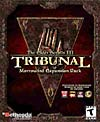
\includegraphics{media/image6.png}

GetScale (float)

SetScale newScale\_float

ModScale scaleChange\_float

If ( doonce == 0 )

Object\_ID-\textgreater SetScale 0.1

Set doonce to 1

endif

These functions are used to determine or modify the scale of a
reference. Any scale you can set must be within (exclusively) 0 and 10
(so you can set it beyond 0.5 and 2, contrary to what was written in the
original description by Bethesda) (info by Mode Locrian). The above
sample script can thus be used to set scale beyond the limits of what
the TES CS itself allows.

\textbf{Notes:} You shouldn't call "setscale" in every frame, at least
not in exteriors or other FPS-critical situations.

The scale will be reset to a value within the 0.5 - 2.0 frame when you
reload. So don't use a done-flag to call it only once. Either call it
regularly (about all 10 frames) or test for "getscale" and reset the
scale when it doesn't fit:

if ( GetScale != 5 )\\
SetScale, 5\\
endif

Another way is to set it in a Tribunal or Bloodmoon start script. This
can be done once, and will make sure the scale is set each time you load
a game. (Forum info / JOG).

Sample script:

A more complex sample script by Bethesda shows how to grow and shrink an
object.

When this script is placed on a reference, activating that reference
gives the user the ability to change that reference's scale.

\lstinputlisting{scripts/scalescript.txt}

\hypertarget{determining-location-relative-position-and-movement}{%
\subsection{\texorpdfstring{\hfill\break
Determining location, relative position and
movement}{ Determining location, relative position and movement}}\label{determining-location-relative-position-and-movement}}

\hypertarget{detecting-if-player-is-indoors-or-outdoors}{%
\subsubsection{Detecting if player is indoors or
outdoors}\label{detecting-if-player-is-indoors-or-outdoors}}

{[}no fix{]} GetInterior (returns Boolean/short)

If ( GetInterior == 1 )

\textbf{Undocumented function!} (Thanks XP-Cagey and Killgore)

This function will return 1 if the current cell is an interior cell and
0 if it is an exterior cell. It will also return 1 if the player is in
an interior acting like exterior (GetWindSpeed can be used to detect a
fake exterior).

The following is a global sample script by Killgore. If you want to try
it out start it by typing "StartScript Outside\_Check" in the console.

\lstinputlisting{scripts/Outside_Check.txt}

\hypertarget{determining-the-players-cell}{%
\subsubsection{Determining the players
cell}\label{determining-the-players-cell}}

{[}no fix{]} GetPCCell, "Cell\_ID" (returns Boolean/short)

if ( GetPCCell "Balmora" == 1 )

Set dream to 1

endif

The GetPCCell function tests for the player's presence in the specified
cell. It returns 1 if the player is in the specified cell, 0 if not.
Partial matches are supported, e.g. GetPCCell, "Vivec" will return true
for the cells "Vivec", "Vivec, foreign quarter waistworks" and "Vivec,
temple", etc.

Sample Script:

This small Bethesda script checks for the PC leaving a certain area
until removing a certain item from an NPC:

\lstinputlisting{scripts/DrothPost.txt}

\hypertarget{distance-of-one-object-to-another}{%
\subsubsection{Distance of one object to
another}\label{distance-of-one-object-to-another}}

GetDistance, "ObjectID" (returns float)

"ObjectID1"-\textgreater GetDistance, "ObjectID2"

This function returns the distance (in units) of one object to another.
In syntax one, that is the distance between the calling object (to which
script is attached to) and the named object. This can be used to trigger
attacks or other events, or simply to roughly determine the player's
whereabouts for use in a script.

Here is a snippet from an original Morrowind script:

; From a script attached to an NPC Ashamanu:

; Ashamanu will give journal entry 60 when player is near

if ( GetDisabled != 1 )

if ( \textbf{GetDistance} Player \textless= 256 )

if ( \textbf{GetDistance} "guar\_white\_unique" \textless= 256 )

if ( GetJournalIndex "MS\_WhiteGuar" \textless= 50 )

Journal "MS\_WhiteGuar" 60

endif

endif

endif

endif

Limitations:

\begin{itemize}
\item
  GetDistance requires that the object given as parameter is placed in
  the gameworld (in the editor) and has references persist checked (or
  is naturally persistent such as an NPC).
\item
  Note that you should use this function only with unique ID's or in
  environments where you exactly know that there is only one instance of
  the ID -- otherwise the Game engine will just grab the first instance
  of the ID it finds and report that distance -- most likely not the
  distance to the object you want. Thus, a script that warns the player
  of the presence of a slaughterfish that is closer than 800 units would
  have to be attached to the ID of the slaughterfish, and check the
  distance to "player" (which is unique), not vice versa.
\item
  If you determine distance to an object you are moving with Move or
  MoveWorld, GetDistance will still report the \textbf{distance to the
  original location} of the object (the one you set in the editor). Use
  GetPos and good ol' Pythagoras (c\textsuperscript{2} =
  a\textsuperscript{2} + b\textsuperscript{2}) to determine distances in
  these instances.
\item
  GetDistance won't work on disabled objects.
\end{itemize}

\hypertarget{determining-an-objects-position-and-facing}{%
\subsubsection{Determining an objects position and
facing}\label{determining-an-objects-position-and-facing}}

GetPos, axis(x/y/z)

Object\_ID-\textgreater GetPos, z

When you are moving objects with the Move/MoveWorld functions described
above, you might want to obtain information on its current whereabouts.
This functions work on Actors and objects. In the following sample
script I used this function to control the movement of a light source (a
fire) to make a fire pit where the flames actually start slowly and die
down in the evening on a daily schedule -- the fire objects original Z
position is 511:

\lstinputlisting{scripts/_HB_Scheduled fire.txt}

GetAngle , axis(x/y/z) (returns float)

If ( Object\_Id-\textgreater GetAngle, z == 180 )

The GetAngle function returns the world angle, not the local angle.
World angles are from 0 to 180 and 0 to -180 (see figure for z axis).

\textbf{Note:} This works on actors and objects, however for the player
(and I assume other actors) only the z axis is relevant - GetAngle, x or
y always return 0.

\hypertarget{line-of-sight}{%
\subsubsection{Line of Sight}\label{line-of-sight}}

GetLOS, ObjectID (returns Boolean/short)

Actor\_ID-\textgreater GetLOS, Player

Undocumented:

GetLineOfSight (returns Boolean/short)

These functions determines whether the calling object has line-of-sight
to the referenced object. It does not seem to work for non-Actor type
objects, as far as I could determine. It does not take facing into
account, so don't take the "sight" part too literally. (See "Is she
looking at me?" in the Tips and Tricks section.)

\textbf{Note}: GetLOS is a very slow function, don't let the script call
it every frame.

\textbf{Sample Script}:

\lstinputlisting{scripts/balynScript.txt}

\hypertarget{section-2}{%
\subsubsection{}\label{section-2}}

\textbf{Note:}

getLOS and getLineOfSight suffer from the same problem with generic NPCs
as getDetected (see below)\\
\protect\hypertarget{_Toc182634542}{}{}\emph{\textbf{Determine whether
an Actor is detected by another Actor}}

{[}no fix{]} GetDetected, "Actor ID" (returns Boolean/short)

If ( GetDetected, Player == 1 )

Returns true if \textbf{any} calling Actor can detect "Actor ID" (thanks
for the correction, ThePal!). This function will return 0 if the Actor
is hidden in some form, e.g. is sneaking successfully, or has an
invisibility or chameleon spell active. According to the helpfile this
is a slow function, do not call it a lot (e.g. make a counter to only
call it every 3 seconds).

\textbf{Sample script:} The player must approach an object undetected --
if not he is "caught"

\lstinputlisting{scripts/jeanneScript.txt}

GetDetected calling an NPC's ID if there's more than one reference in
the game will return nothing. For example:

getDetected, "fargoth"

will return 1, but:

GetDetected "Imperial Guard"

Returns nothing. (Not 0, it doesn't return a value). However if you
reference an exact NPC:

GetDetected "Imperial Guard00000002"

A value is returned.

(Forum info / Fliggerty )

\hypertarget{determining-when-the-pc-leaves-a-cell}{%
\subsubsection{Determining when the PC leaves a
cell}\label{determining-when-the-pc-leaves-a-cell}}

{[}no fix{]} CellChanged

If ( CellChanged == 1 )

CellChanged returns 1 for one frame when player changes cells. It
doesn't return 1 for scripted teleporting or magic teleporting.
CellChanged returns true almost immediately after the player changes
cells. This means a local script running in an interior cell won't fire
when the user leaves a cell, but rather when the player enters the cell.

Scripted teleporting may trigger CellChanged if the script is global or
targeted (local scripts will not trigger it). (Forum info / Zennorious,
Tamandra)

Note:

CellChanged doesn't always trigger, even if the player enters the cell
via a normal teleport door. Possibly scripts running in the cell can
have some effect on this, somehow. ForceGreeting seems to muck it up in
particular (and no there wasn't a menumode return in that script).

\textbf{Sample Script:} In the SlaveScript, which governs freeing slaves
in the game, CellChanged is the trigger to disable the slave -- the
slave has left for a better future:

\lstinputlisting{scripts/SlaveScript.txt}

another nice example is the Gateway Haunt's script. This spectre always
comes back just when you are not watching:

\lstinputlisting{scripts/ResurrectHaunt.txt}

\hypertarget{detect-player-traveling}{%
\subsubsection{Detect player traveling}\label{detect-player-traveling}}

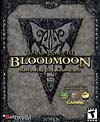
\includegraphics{media/image7.png}

{[}no fix{]} GetPCTraveling (returns boolean)

if ( GetPCTraveling == 1 )

Bloodmoon adds a functions to check whether the PC is traveling (i.e. on
a Silt Strider). Will return 1 if traveling/in jail, zero otherwise.
This is used in the werewolf change script to stop the PC from changing
if either of these are true:

if ( PCWerewolf != 1 ) ; DON' RUN IF PLAYER ISN'T WEREWOLF

return

endif

if ( \textbf{GetPCinJail} == 1 )

return

endif

if ( \textbf{GetPCTraveling} == 1 )

return

endif

\hypertarget{triggers-for-actors-standing-on-an-object}{%
\subsubsection{Triggers for Actors standing on an
object}\label{triggers-for-actors-standing-on-an-object}}

GetStandingPC (returns Boolean/short)

returns 1 if PC is standing on it.

GetStandingActor (returns Boolean/short)

returns 1 if ANY Actor (including PC) is standing on it.

If ( Object\_Id-\textgreater GetStandingPC == 1)

{[}\ldots{} trigger horrible trap{]}

endif

These are great functions to trigger events, especially for interior
cells. It is also an excellent function to build traps. You can make an
"activator" object using the nif files of any static object (hallway,
carpets etc.), and trigger certain events once the player (or another
Actor) steps on that object.

My sample script is used to light fires in a hall on as soon as the
player steps on a particular piece of floor:

\lstinputlisting{scripts/HBHallLighting.txt}

HB\_hallfire is a global variable, used to turn on the fire. This is the
script for the fire:

\lstinputlisting{scripts/HBHallfireon.txt}

\hypertarget{hurting-an-actor-standing-on-an-object}{%
\subsubsection{Hurting an Actor standing on an
object}\label{hurting-an-actor-standing-on-an-object}}

HurtStandingActor, float\_HP/s

HurtStandingActor -3

Object\_ID-\textgreater HurtStandingActor 1

Float hurt\_variable

HurtStandingActor, hurt\_variable

This function affects the health of an Actor (including the PC) that
stands on the object. Positive values will reduce health, negative
values heal (hitpoints per second). Using negative values will modify
your health even beyond your normal maximum health, so be careful to
test this if you want to use this function this way. This function
accepts float variables.

\textbf{Sample script:} The effect is probably best known from the lava
fields:

\lstinputlisting{scripts/lava01.txt}

\hypertarget{object-collision-functions}{%
\subsubsection{Object Collision
Functions}\label{object-collision-functions}}

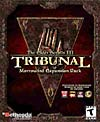
\includegraphics{media/image6.png}

GetCollidingPC (returns Boolean/short)

GetCollidingActor (returns Boolean/short)

if ( GetCollidingPC == 1 )

HurtCollidingActor, damage\_enum

HurtCollidingActor, 100

Object\_ID-\textgreater HurtCollidingActor, 100

These functions go on an object to allow it to interact with Actors
colliding with it. GetCollidingPC returns 1 if the PC is currently
colliding with the object and 0 otherwise. GetCollidingActor works the
same as the PC version of the function but will return 1 if any Actor
(other than the PC) is colliding with the object. HurtCollidingActor
lowers the colliding Actor's health Damage points every second.

\textbf{Note:} An object has to have collision to trigger these
functions, so if you can walk through the object, none of these
functions will trigger.

Sample script:

When this script is placed on an object, any Actor touching that object
will take damage. A different message is given depending on whether the
Actor is the PC or someone else.

\lstinputlisting{scripts/hurtActor.txt}

\hypertarget{section-3}{%
\subsection{}\label{section-3}}

\hypertarget{section-4}{%
\subsection{}\label{section-4}}

\hypertarget{checking-activation-of-an-item-and-activating-it}{%
\subsection{Checking activation of an item and activating
it}\label{checking-activation-of-an-item-and-activating-it}}

An item is usually activated when you press the spacebar to "use" it.
Most items have a standard action that is performed when they are
activated: Doors open, chests display their content, Actors initiate
dialogue etc. The OnActivate function allows you to intercept the
standard action and do something else or check a condition first:

OnActivate

If ( OnActivate == 1 )

This get set to one for one frame when the object is activated.
OnActivate resets itself as soon as the function is called, so only one
script can report OnActivate successfully, and you should only have one
OnActivate call in your script at each moment. OnActivate short-circuits
the normal behavior of the object -to perform the standard action of the
object once OnActivate has been called, you have to use the activate
command:

Activate

activate (if script is on the object to activate)

Activate can be used to trigger the standard action of an object, after
OnActivate has been called.

\textbf{Standard actions called by Activate are:}

Doors -\textgreater{} Open (Possibly broken in Original MW, with
v1.6.1820 it definitely works).

LoadDoors -\textgreater{} Open (If used with OnActivate)

Containers -\textgreater{} Open (show contents)

Books/scrolls -\textgreater{} Display text to read.

Activators -\textgreater{} Nothing

Actors -\textgreater{} Dialogue

Weapon -\textgreater{} Pick up

Armor -\textgreater{} Pick up

Miscellaneous -\textgreater{} Pick up

Not tested, but I assume:

Equip. Lights -\textgreater{} Pick up

Other Lights -\textgreater{} Nothing

Probes -\textgreater{} Pick up

Apparatus -\textgreater{} Pick up

Example script:

The following script demonstrates the use of OnActivate nicely. It is
attached to a container object, a chest that does NOT advertise its trap
like the normal in-game ones do:

\lstinputlisting{scripts/Trap_script.txt}

\textbf{Notes}: According to my testing, the activate function can not be used by itself, without OnActivate in the same script. The OnActivate and Activate functions can be in different parts of the script, though. However, Activate will not work before OnActivate has not at least been called once. There have been reports that the object also must have been manually activated at least once within the last 72 hours, so apparently the game eventually forgets that OnActivate has been called previously. Containers require manual activation each load session (forum info / Phaedrus). Play around with this testscript (I had it attached to a door) to
see for yourself:

\lstinputlisting{scripts/GBG_closing_door.txt}

There have also been various reports about difficulties with on
OnActivate in general, in my experience, avoiding to use more than one
OnActivate in a script is the safest way to go. Also be aware that for
items in your inventory, OnPCEquip may be the function to use instead of
OnActivate, as OnActivate does not get called by moving the item over
the Player icon.

Info from the UESP: There is an undocumented feature in the Activate
function by specifying the player after the function, for example:

\lstinputlisting{scripts/RemoteContainer.txt}

If the container is persistent (references persist) this script should
open the container wherever the player is. This is a great way to create
'carryable' containers by attaching a script similar to the above to a
ring or similar item.

\hypertarget{locking-and-unlocking-doors-or-chests}{%
\subsection{\texorpdfstring{\hfill\break
Locking and Unlocking doors or
chests}{ Locking and Unlocking doors or chests}}\label{locking-and-unlocking-doors-or-chests}}

Lock, short\_enum\_locklevel

Unlock

My\_Door-\textgreater Lock, 50

GetLocked (returns Boolean/short)

If ( GetLocked == 1 )

Unlock

Endif

(only Door and container objects)

These functions are used to lock and unlock doors or containers. The
GetLocked function returns 1 when the calling object is locked. Lock
locks the object with the lock level specified (0-100). Lock 0 has an
odd effect though. The door/container will be neither openable nor
pickable. Unlock removes any lock, regardless of lock level.

Example script:

Here is a sample script by qwert, which makes a chest function as a
security skill-training device by constantly relocking it:

\lstinputlisting{scripts/PC_Security_Skill_Trainer.txt}

\hypertarget{animating-objects}{%
\subsection{Animating objects}\label{animating-objects}}

There is a group of functions that allows you to play specific
animations that are defined in a model (.nif file). You can find out
about the animation group names by loading a model into the preview
window and then skipping through the different animation groups or by
looking at "base animation" windows in the "Character" menu. An
excellent summary of Actor animation groups can be found here:

\href{http://morrowind.preik.net/animationgroups.html}{http://www.preik.net/morrowind/animationgroups.html}

but only the ones listed in the base animation window can be called by
this function. Additional animations can be loaded to a model via the
animation button in the object window. See the Dancing girls in "Suran,
Desele's house of earthly delights" for an example.

Not all models have animation groups, but the different banners (under
activators) are good examples to see what is meant (see example below).
Examples for GroupName are: idle, idle2, idle3, walk, etc.

These functions do not work on the player character.

PlayGroup, GroupName, {[}Flags{]}

PlayGroup, walk, 1

Plays the animation group defined by GroupName. Optional flags can be
used to start the group in different ways (see below).

LoopGroup, GroupName, Number\_enum, {[}Flags{]}

Plays the animation group defined by GroupName. The animation will be
looped the number of times specified, and then return to the Idle
animation. Optional flags can be used to start the group in different
ways (see below).

Flags:

\emph{0 = Normal}

The current animation will finish its full cycle, and the new animation
will start from its beginning.

\emph{1 = Immediate Start}

The current animation will stop regardless of the frame it is on, and
the new animation will start from its beginning.

\emph{2 = Immediate Loop}

The current animation will stop regardless of the frame it is on, and
the new animation will start at the beginning of its loop cycle.

\textbf{Note:} With Bloodmoon installed (not necessarily Bloodmoon.esm
selected) some of NPC animations are crosswired. When called from
console, they may look correct, but if you insert
NPC-\textgreater PlayGroup, group, 1 into the script, you may be
unpleasantly surprised to see a different animation than you expected
(Forum info / Kir). You may have to experiment to find the correct
animation (Check out the info in the section on AIWander for a list of
NPC idle movements, or download the NPC Animation Explorer mod to see
all possible animations ingame:
\url{http://www.angelfire.com/rpg2/mad_weather/animexp.htm}).

\textbf{Note:} NPCs may play a different animation on the upper body
while the lower body does the scripted animation. This may also be
version-dependent(?), but in any case these functions appear to be
unreliable when used with NPCs.

Example Script:

This original script is attached to all the outside banners and makes
them move differently depending on the weather:

\lstinputlisting{scripts/OutsideBanner.txt}

SkipAnim

Causes the current animation to not be played for this frame.

\hypertarget{enabling-and-disabling-objects}{%
\subsection{Enabling and disabling
objects}\label{enabling-and-disabling-objects}}

Enable

Disable

"ObjectID"-\textgreater enable

GetDisabled (returns Boolean/short)

If ( GetDisabled == 1 )

Return

Endif

The \emph{Disable} function makes an object completely vanish from the
game world, meaning it's neither rendered nor processed (attached
scripts are still active, however). The \emph{Enable} function makes a
disabled object visible and processed again. \emph{GetDisabled} (returns
1 if object is disabled) can be used to obtain the current status of an
Object. These functions are very powerful and could e.g. be used to swap
different models of statics (normal house replaced by house burnt to the
ground, etc). It is e.g. used for the stronghold building process.

Note that disable should not be called every frame, as this will cause a
drop in framerate. Instead, use GetDisabled or some other condition to
ensure the object is disabled only when necessary.

Example script:

An example from the game is the SlaveScript that makes freed slaves
vanish once the player leaves the cell:

\lstinputlisting{scripts/slaveScript.txt}

\textbf{Caution: disabling lights}

There seems to be a game engine issue with disabled lights -- Actors and
some other types of objects still seem to be illuminated, while the
world around is not. I have not thoroughly tested if this can be
avoided, but a suitable workaround is to physically remove the light to
a remote location (e.g. a few meters below the floor) instead of
disabling it. Another trick comes from Indigo: If you enable a light
that is set to "negative" (which means its generating darkness instead
of light) after you disable the normal light, the illumination problem
goes away.

\textbf{Note:}

When you are in an exterior cell (haven't checked with interiors, but
presumably it applies in interiors as well) any object you disable in
the loaded cells while you are in that cell will retain its collision
properties in the game world until the next time that exterior cell is
loaded - i.e. you disable a fence piece through a script where that
fence piece is in the same exterior cell as your PC. You still can't
walk through the area where the fence piece is disabled until you exit
and reenter that exterior cell. Similarly, you subsequently reenable
that fence piece that was disabled when your PC entered that exterior
cell. You can walk right through that fence piece until the next time
that exterior cell is reloaded by the game.

To fix this use the "FixMe" command in your script after you disable or
enable a game object that exhibits collision. You should check that you
are in the same exterior cell as the game object before you execute the
FixMe command - if you aren't you don't need FixMe. This is useful in
global scripts that enable or disable objects with references persist so
you could be in any cell when the object is enabled or disabled. Using
FixMe will cause your PC to also move 128 game units (hardly noticeable
in most cases other than as a "stutter") when it executes but since
there is no other script command that reloads a cell that is something
you will have to live with. Using FixMe will cause the collision to be
reset for the cell FixMe reloads so is a way to immediately fix
collision on script enabled/disabled objects. (Forum info /
\href{http://www.bethsoft.com/bgsforums/index.php?showuser=370208}{Rougetet})

\hypertarget{section-5}{%
\subsubsection{}\label{section-5}}

\hypertarget{deleting-a-reference-completely}{%
\subsubsection{Deleting a reference
completely}\label{deleting-a-reference-completely}}

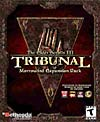
\includegraphics{media/image6.png}

{[}no fix?{]} SetDelete flag\_enum

SetDelete 1

The SetDelete function can be used in combination with Disable to remove
an object more completely. SetDelete 1 marks a reference for deletion
and SetDelete 0 clears that flag. This can be useful in optimization.
Certain objects have scripts on them which simulate picking them up by
disabling the activated reference and adding a new object to your
inventory. This leaves an ever-present, but disabled, reference at that
location (which eats up memory and processor time since the script on
the disabled reference is still run every frame). If the reference is
marked for deletion then it is essentially gone. If the reference came
from the master file, it is still there but knows it shouldn't be so has
no art and no scripting. If was created in game, it will actually be
deleted.

\textbf{Notes and cautions:}

SetDelete will crash Morrowind if there is any other function operating
on the object in the same frame. It will also crash if the object emits
sounds (or plays animations with linked sounds) and is disabled and
deleted in the same frame (forum info / JOG).

This Script \textbf{will crash}:

\lstinputlisting{scripts/_spell_effect01.txt}

A solution is to use first disabling the object and then using
GetDisabled and Return to safely delete the object:

\lstinputlisting{scripts/_spell_effect02.txt}

Another solution was proposed by Soralis, using a local variable
"deletobj" as a flag:

if ( deleteobj = 1 ) ;Local variable, set when you want to delete

if ( deletetimer == 0 )

Disable

endif

if ( deletetimer \textless{} 10 )

set deletetimer to ( deletetimer + 1 )

endif

if ( deletetimer == 10 )

\textbf{SetDelete}, 1

endif

Return

endif

Always call SetDelete from a local script assigned to the object you
want to remove. Never use Object-\textgreater SetDelete 1 as this
usually causes crashes when Morrowind is running. However, starting a
targeted script on the object and then using SetDelete in that script
works fine.

Don't delete items in inventory: this results in incorrect encumbrance.
If necessary, Drop can be used to remove the item from inventory before
deletion.

It has been reported that magic effects can cause problems with
SetDelete (forum info / Dan\_Wheeler). I (melian) am not sure exactly
what this refers to, but I do know that if an NPC is deleted too quickly
after another NPC casts a spell on it (scripted cast), the game will
crash. If this causes you problems, use a timer to wait before deleting
the object (you may need to wait a few seconds).

\hypertarget{dont-save-changes-to-an-object}{%
\subsection{\texorpdfstring{\hfill\break
Don't save changes to an
object}{ Don't save changes to an object}}\label{dont-save-changes-to-an-object}}

DontSaveObject

Call this function if changes to the object are not to be saved to the
savegame.\\
Use DontSaveObject on objects that:

1. Can be enabled/disabled during the game, such as the stages of
building a stronghold.

2. Objects that might be moved, such as rideable objects.

By using DontSaveObject you will avoid that annoying "save game data has
changed" error message that will occur when load a saved game and the
object's state has changed, ie: it has moved, or has been
disabled/enabled. This is due to the fact that object data is stored in
the save game data, such as if the object is enabled or disabled, or if
it has been moved (like a rideable object) (Forum info / IndigoRage).

In the original game, it's used in the SignRotate script and the
following one:

Sample Script:

\lstinputlisting{scripts/diseaseAscended.txt}

\hypertarget{scripting-npcs-ai-and-movement}{%
\section{\texorpdfstring{\hfill\break
Scripting NPCs: AI and
Movement}{ Scripting NPCs: AI and Movement}}\label{scripting-npcs-ai-and-movement}}

\hypertarget{make-an-npc-walk-to-a-new-location}{%
\subsection{Make an NPC walk to a new
location}\label{make-an-npc-walk-to-a-new-location}}

AiTravel, float\_enum\_x, float\_enum\_y, float\_enum\_z, {[}reset{]}

Actor-\textgreater AITravel, 1359, 2700, 1045

To make an NPC walk between different defined places in the game world
you use the AITravel function.

The variables x, y, z are world coordinates. You can determine these by
moving your camera to the desired endpoint of the movement or by
selecting a path grid point or an object nearby coordinates are
displayed below the object window. The usage of the optional reset flag
is unknown.

When using this function in scripts it is important to provide
conditions where the AI package is called only once. Consider the
following NPC bound script

\lstinputlisting{scripts/Travel01.txt}

The previous script will not work, as the script ``fires'' continuously,
and the effect is that the NPC freezes and never performs the desired
movement.

\lstinputlisting{scripts/Travel02.txt}

This should work; the NPC will wander to the designated coordinates as
soon as his script becomes active, meaning as soon as his cell is
loaded.

\hypertarget{checking-whether-an-npc-has-performed-his-movement}{%
\subsubsection{Checking whether an NPC has performed his
movement}\label{checking-whether-an-npc-has-performed-his-movement}}

GetAIPackageDone (returns Boolean/short)

if ( GetAIPackageDone == 1 )

{[}do something{]}

endif

To check whether an NPC has arrived at his location you can use the
\emph{GetAIPackageDone} function. This function returns 1 for one frame
when the current AI package has finished.

Use this to perform a check whether a movement has been finished. The
following script is an example of how to link several \emph{AITravel}
commands within one script, using a state variable and an
\emph{if-elseif} structure:

\lstinputlisting{scripts/TravelLoop.txt}

Good examples of scripting using \emph{AITravel} are also found in the
``lookoutscript'' (Fargoth hiding his treasure) and the CharGenWalkNPC
script (The guard that walks you through the ship at the beginning of
the game). Or look at my "Traveling Merchants" plugin for true AITravel
madness !

If you plan on using this function extensively you should be aware of
the following problems: When you leave a cell with an Actor that is just
performing its AITravel command, or if you rest, the script will never
detect the \emph{GetAIPackageDone} signal, meaning your NPC gets stuck
on its path once you return or finish sleeping. The following simple
code can be used to get the script going again (this is for the above
script)

% Excerpt from external script

; *************** Stalled Script rescue - recovers script after leaving
a cell or resting

If ( Player-\textgreater GetDistance, HB\_adros\_darani \textless{} 5000
)

if ( GetCurrentAIPackage == -1 ) ; check for idleness

set timeout to ( timeout + GetSecondsPassed )

if ( timeout \textgreater= 3 ) ; wait some time.

; Short instances of idleness always occur

set state to ( state - 10 ) ; stall will occur at ; AIPAckageDone - jump
to "wander" again.

set timeout to 0

endif

else

set timeout to 0

endif

endif

\hypertarget{make-an-actor-turn-or-face-a-certain-direction}{%
\subsection{Make an Actor turn or face a certain
direction}\label{make-an-actor-turn-or-face-a-certain-direction}}

Face x\_enum, y\_enum

"ActorID"-\textgreater Face, -1334, 334

To my knowledge this function does not accept variables (at least under
version 1.6.1820), but there have been reports that it did - possibly
this is version dependent. This function Makes an NPC face towards a
specified x/y coordinate. Apparently interrupts current animations.
Using this on wandering NPCs makes them stop, face wherever, then
continue on wherever they were wandering to, as soon as the facing
movement is over. (Forum info / JOG, Dan\_Wheeler).

\hypertarget{define-random-actor-movement}{%
\subsection{Define random Actor
movement}\label{define-random-actor-movement}}

AiWander, range\_enum, duration\_enum, time\_enum, {[}idle1{]},
{[}idle2{]}, {[}idle3{]}, \ldots{[}idle9{]}, {[}reset{]}

"Actor\_ID"-\textgreater AIWander, 512, 5, 0, 0, 20, 0, 0, 10, 30, 0, 0,
0

This is the random movement algorithm that most of the NPCs in the game
are using. The NPC travels along the path grid, changes direction
randomly, and performs idle movements in between.

\begin{itemize}
\item
  Range: determines the distance the Actor or creature will roam from
  his origin.
\item
  Duration: probably the time (in hours) the mob will perform the
  package (before it is reset, which seems to happen if you leave or
  sleep, not sure?)
\item
  time: presumably determines the start time for the package if it has a
  duration
\item
  {[}idle1{]}, \ldots{[}idle9{]}: chances of idle movements.\\
  \strut \\
  The Idles are (as tested in game):
\item
  Human male:\\
  Idle1: Stand still\\
  Idle2: Shifting weight from one leg to the other\\
  Idle3: Looking behind\\
  Idle4: Scratching head, shake head\\
  Idle5: Shifting clothing or armor on shoulder\\
  Idle6: Yawning and stretching\\
  Idle7: Looking at fingers and looking around furtively\\
  Idle8: Putting hand to chest, as if having heartburn\\
  Idle9: Reaching for weapon, then touching head
\item
  Human female - as above but:\\
  Idle5: Hand on hip
\item
  Khajiit female - as Human male but\\
  Idle9: Scratching head, shaking head
\end{itemize}

To let an Actor stand in one spot you can use: AIWander, 0, 0, 0

\textbf{Note:} The number of idles and some of the descriptions were
listed wrongly in previous versions (corrected with
8\textsuperscript{th} edition - credits go to Whoopa).

Here is an \textbf{example script} that displays all idles in series
(this my be useful to check out which ones you want your NPC to use):

\lstinputlisting{scripts/Animtest.txt}

\hypertarget{making-actors-activate-objects}{%
\subsection{\texorpdfstring{\hfill\break
Making Actors activate
objects}{ Making Actors activate objects}}\label{making-actors-activate-objects}}

AiActivate "Object ID"

AiActivate ObjectID {[}reset{]}

Actor-\textgreater AIActivate "Object"

In the words of Bethesda: "This package tells the Actor to activate the
specified ObjectID. A powerful and admittedly underutilized and
undertested package."

In standard Morrowind this function appeared to be mostly broken, except
for making an NPC quaff a potion. \textbf{With Tribunal} it seems to
have been fixed, at least to some extent. I could successfully use it to
get an NPC to pick up a weapon, open a normal door and go through a load
door. LoadDoors only work if the door marker it teleports to is in the
same interior cell, or within the loaded (PC's current and surrounding)
cells in exterior cells -- otherwise the game crashes. I also tested it
successfully with an activator (switch to open Ghostgate).

The usual precautions with AI functions apply (make sure the Actor is
not too far away, have a good AI grid in place, make sure nothing can
get in the way, etc.). Although not thoroughly tested, I didn't seem to
get an \emph{AIPackageDone} signal, but other conditions can be
constructed (see examples below) to set the NPC to a different AIPackage
again.

\begin{longtable}[]{@{}
  >{\raggedright\arraybackslash}p{(\columnwidth - 2\tabcolsep) * \real{0.25}}
  >{\raggedright\arraybackslash}p{(\columnwidth - 2\tabcolsep) * \real{0.75}}@{}}
\toprule
\begin{minipage}[b]{\linewidth}\raggedright
Object Type
\end{minipage} & \begin{minipage}[b]{\linewidth}\raggedright
Activation
\end{minipage} \\
\midrule
\endhead
NPC & Activating NPC will approach and circle the target NPC \\
Container & Opens \\
Door & Opens \\
Load door & Opens/teleports (same cell only) \\
Weapon, armor, misc., etc & Picks up \\
Book/Scroll & Reads \textless meaning what to an NPC?\textgreater{} \\
Activators & Execute as defined by script. If the activator doesn't have
an OnActivate block (or doesn't have a script), the Actor will try to
activate it anyway, in much the same way as 'activating' NPCs (approach
and circle). \\
\bottomrule
\end{longtable}

\textbf{Note:}

If you place the object to be activate too high, the NPC will still
approach and circle underneath it.

\textbf{Sample Script:} these are just a few testing scripts I made.
They show how you can set conditions to determine when the NPC has
finished his action.

\lstinputlisting{scripts/TT_opendoor.txt}

\lstinputlisting{scripts/TT_pickmace.txt}

\lstinputlisting{scripts/TT_openloaddoor.txt}

\hypertarget{following-and-escorting}{%
\subsection{Following and Escorting}\label{following-and-escorting}}

AiFollow, "Actor ID", duration\_f\_enum, x\_f\_enum, y\_f\_enum,
z\_f\_enum, {[}reset{]}

AiFollowCell, "Actor ID", "Cell ID", duration\_f\_enum, x\_f\_enum,
y\_f\_enum, z\_f\_enum, {[}reset{]}

Actor-\textgreater AIFollow, "Mob2ID", 0, 0, 0, 0

The "Follow" AI-package makes an Actor closely follow another. You can
use this to make an NPC or creature follow the player, but you can also
use it to make NPCs and creatures form a caravan. The following excerpt
from one of my own scripts shows the unconditional use of the function:

elseif ( state == 20 )

HB\_guar\_pack\_adros\_-\textgreater{}\textbf{AIFollow},
HB\_adros\_darani, 0, 0, 0, 0

AITravel -8144, -19409, 728 ;new coords point 1

set state to 30

Since there is no duration or destination location given, the guar will
follow the NPC until another command is given. As with other
AI-commands, make sure you set conditions so that each AIFollow command
is issued only once, not every frame.

The duration, CellID and x, y, z destination coordinates set conditions
that once fulfilled will terminate the AIPackage (which you can test
with the GetAIPackageDone function as describe for AITravel above). The
AiFollowCell function allows you to set an interior cell as the
destination.

The meaning of the optional reset option is currently unknown.

AIEscort, "Actor ID", duration, x, y, z, {[}reset{]}

AIEscortCell, "Actor ID", "Cell ID", duration, x, y, z, {[}reset{]}

This function makes an Actor lead another actor or the player to a
certain point. The Actor will wait for the follower if the distance
becomes too great, and will resume its path when the follower approaches
again (Thanks to Kir for this info). You see an \textbf{example} of this
in character generation: the guard who escorts you up from the ship's
hold to the ramp on the second level. (Thanks to MisterSmileyFaceDude).
The meaning or use of {[}reset{]} is unknown.

\hypertarget{checking-which-ai-package-is-currently-executed}{%
\subsection{Checking which AI package is currently
executed}\label{checking-which-ai-package-is-currently-executed}}

For complex Actor scripting it might be valuable to know which AI mode
is currently active and make script actions dependant on it.

GetCurrentAIPackage (returns short)

If ( GetCurrentAIPackage == 2 )

{[}do something{]}

endif

The returned values are:

\begin{longtable}[]{@{}
  >{\raggedright\arraybackslash}p{(\columnwidth - 2\tabcolsep) * \real{0.72}}
  >{\raggedright\arraybackslash}p{(\columnwidth - 2\tabcolsep) * \real{0.28}}@{}}
\toprule
\endhead
None & -1 \\
Wander & 0 \\
Travel & 1 \\
Escort & 2 \\
Follow & 3 \\
Activate & 4 \\
Pursue & 5 \\
\bottomrule
\end{longtable}

\hypertarget{section-6}{%
\paragraph{}\label{section-6}}

Casey Tucker wrote a few interesting notes about Morrowind's AI system:

\emph{These are a few notes on Morrowind's AI system, as much for myself
as for anyone wishing to look them over. The most I noticed the AI is
incredibly stubborn. There are quite a few unpredictable script
functions that deal with AI. I find that the AIFollow is actually the
most stable of them.}

\emph{\hfill\break
When working on "The Triumvirate" quest/war mod, if the player went to
Dragonhold Castle to join the Legion, I had to have the player's
Imperial Centurion, Sensius Tanarii, show the player where his barracks
room is.}

\emph{\hfill\break
Initially I had Sensius follow the player until you wandered around long
enough to find your barracks room. Sensius would confirm the location
and disappear, once Proximus Taiatius, (your legionary roommate) noticed
you.}

\emph{(GetTarget Player == 1 Usually works - For the desired effect,
GetDistance is more accurate.)}

\emph{\hfill\break
So, that was sort of the opposite of I wanted. I wanted Sensius to take
the player to their room. When I first actually thought of this, I tried
thinking of several ways to get an NPC to "AiEscort" through several
cells to the given coordinates. Let me tell you of my findings on
AIEscort. It's either broken, works only in exterior cells, or I was
doing something wrong. Regardless, I noticed that the NPC did not budge
at all from their location, though they WERE set to guard the player.
Upon further research, I saw that during the CharGen process, when the
prison ship guard appears to be escorting you to the door, Bethesda
actually used AIWander, making checks to see if the player was following
or not.}

\emph{From this I drew the conclusion that AITravel would be so much
more convenient and stable. I only use AIEscort to get a stationary
actor to guard the player if they came under attack. Useful for battle
scenes when you want it to appear that two forces are fighting each
other, without having an entire side follow the player. About mass
battles... I will lead into that later.}

\emph{\hfill\break
First, I must explain how to get an NPC to escort a player, from point
A: an interior cell, through several interior and exterior cells, to
point B: also an interior cell. First things first.. we don't want the
NPC to get stuck. You'll need some pathgrids. A few notes about
pathgrids: the NPC doesn't seem to care about the gridpoints' Z
coordinate {[}This doesn't appear to be correct. See notes below{]}.
That's a very good thing. Pathgrids are like magnetic roads. The NPC is
seemingly "magnetically attracted" to that pathgrid, and their
AIWandering, AITraveling, and AIFollowing will follow along those grids.
To see how these grids work, go in-game, to Ebonheart or another
semi-crowded city, and type in the console: 'TPG'. That will show the
pathgrids - you'll see the NPC's walking between the two yellow "rails"
that are drawn out, as if they were trains. An NPC will reluctantly pull
away from a pathgrid if led so by the player, need to walk around
something blocking their way, chasing someone/thing, and such
scenarios.}

Now that I got pathgridding done, I noticed another thing. AITravel is
not "unstable" per se, but not very reliable. Two factors come into play
here, that dictate if the NPC will blatantly ignore it's orders or do as
told. The first, I noticed, was the AI distance setting, changeable by
FPS optimizer or in-game menu. Makes sense. However, the next one is
rather annoying. The NPC cannot get distracted or their travel will
stop. This means you'll have to set their "Hello" distance to 0 during
their little stroll, otherwise they will stop and greet the player
instead.

\emph{\hfill\break
Now we come to the point where the NPC reaches a load door through
cells. The game will CTD if the NPC activates it. Here is a snippet of
an "escort" script I wrote, that gets the NPC through a load door.}

\lstinputlisting{scripts/Sensius_Escort_Script.txt}

That should explain how it would work. Coordinates are often more
reliable than a "GetAIPackageDone" function, mainly because that
function is easily broken by several factors.

Some notes on the notes (!)

\begin{itemize}
\item
  It's been reported by others (and I've found myself) that the z-pos of
  pathgrid nodes \textbf{does} matter (at least in interiors): if a node
  isn't well above the floor the actor can get "stuck" at that point and
  refuse to move past it.
\item
  AIEscort has been used successfully by a number of modders (and in
  Bethesda's scripts, e.g. CharGenWalkNPC). That's not to say it's
  without problems, but it is certainly useable. However, since AIEscort
  may not be viable in some circumstances, the above notes may help you
  develop an alternative approach should one be necessary.
\end{itemize}

\hypertarget{forcing-sneak-movement}{%
\subsection{Forcing sneak movement}\label{forcing-sneak-movement}}

ForceSneak

ClearForceSneak

"Actor\_ID"-\textgreater ForceSneak

GetForceSneak ( returns Boolean/short)

If ( "actor\_ID"-\textgreater GetForceSneak == 1 )

The \emph{ForceSneak} command puts the Actor in sneak mode, all movement
will be performed in sneaking. \emph{ClearForceSneak} terminates
\emph{ForceSneak} mode. Unfortunately there does not seem to be a
corresponding command to force running (added with Tribunal).
\emph{GetForceSneak} returns one if \emph{ForceSneak} mode is active on
the calling Actor. Check the LookoutScript script for an example. Here's
a snippet:

elseif ( walkstate == 2 )

Fargoth-\textgreater ForceSneak ; enter sneak mode

Fargoth-\textgreater AiTravel -11468.595,-71511.531,173.728 ;goes to
tree

set walkstate to 3

elseif ( walkstate == 3 )

if ( Fargoth-\textgreater GetAiPackageDone == 1 )

;Fargoth-\textgreater Equip "torch\_infinite\_time\_unique"

set walkstate to 4

;MessageBox "SHOULD BE AT TREE"

endif

elseif ( walkstate == 4 )

set timer to timer + GetSecondsPassed

Fargoth-\textgreater{}\textbf{ClearForceSneak} ; terminate sneak mode

Fargoth-\textgreater AiWander 0 0 0 0 0 0 0 0 0

if ( timer \textgreater{} 3 )

Fargoth-\textgreater{}\textbf{ForceSneak} ; reenter sneak mode

Fargoth-\textgreater AiTravel -11410.590,-72057.188,133.644 ;goes to
wall

set walkstate to 5

endif

\hypertarget{forcing-running-and-jumping-tribunal-npc-movement-functions}{%
\subsection{\texorpdfstring{\hfill\break
Forcing running and jumping: Tribunal NPC Movement
Functions}{ Forcing running and jumping: Tribunal NPC Movement Functions}}\label{forcing-running-and-jumping-tribunal-npc-movement-functions}}

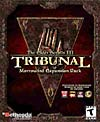
\includegraphics{media/image6.png}

ForceRun

ClearForceRun

GetForceRun (short)

ForceJump

ClearForceJump

GetForceJump (short)

ForceMoveJump

ClearForceMoveJump

GetForceMoveJump (short)

These functions all control the specified NPC's movement. The ForceRun
function makes the NPC always run when they move, the ForceJump function
makes the NPC constantly jump, and the ForceMoveJump makes the NPC
always jump when they are moving. The Get versions of the functions
return one if the specified NPC currently is forced into the given
action and zero otherwise. The Clear functions are used to turn forced
movement modes off. An NPC can only be forced to do one movement at a
time. The priority for forced movement is Sneak \textgreater{} Running
\textgreater{} Jump \textgreater{} MoveJump.

Sample Script:

This script lets an object control the movement type of Athlete, an NPC
set to Travel endlessly in a four-point square.

\lstinputlisting{scripts/AthleteControl.txt}

\hypertarget{detecting-players-action-running-jumping-sneaking}{%
\subsection{Detecting players action: running, jumping,
sneaking?}\label{detecting-players-action-running-jumping-sneaking}}

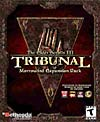
\includegraphics{media/image6.png}

{[}no fix{]} GetPCSneaking (short)

{[}no fix{]} GetPCRunning (short)

{[}no fix{]} GetPCJumping (short)

if ( GetPCRunning )

These functions returns 1 if the PC is performing the appropriate action
and 0 if he is not. Since Morrowind doesn't have functions to directly
test for keyboard input, these functions provide an alternative to check
if the player has a certain button pressed. They have accordingly been
used extensively for control purposes, e.g. for movable ships, ridable
creatures, or in my climbing mod.

Sample script:

When this script is placed on an NPC, and the player has an item
equipped called ``scissors'', MessageBox warnings will be given based on
the player's current actions.

\lstinputlisting{scripts/momscript.txt}

\hypertarget{detect-combat-readiness}{%
\subsection{Detect combat readiness}\label{detect-combat-readiness}}

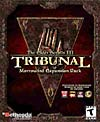
\includegraphics{media/image6.png}

GetWeaponDrawn (short)

GetSpellReadied (short)

if ( player-\textgreater GetWeaponDrawn )

These functions can be used to determine whether or not an Actor has
their weapon out or whether or not they have a spell readied for
casting.

Sample Script: This global script gives notification messages based on
the player's weapon and spell states.

\lstinputlisting{scripts/player_notifications.txt}

\textbf{Note:} GetWeaponDrawn will return 0 at some unusual times; when
a lock pick or probe is removed through scripting or when it is broken,
GetWeaponDrawn will return 0 for a few frames before you switch to
Hand-to-Hand. When fighting Hand to Hand, when you equip or remove a
piece of armor or clothing, GetWeaponDrawn will return 0 briefly.\\
Thanks to Björn and DinkumThinkum respectively for pointing this out.

\hypertarget{section-7}{%
\subsection{}\label{section-7}}

\hypertarget{making-someone-fall}{%
\subsection{Making someone fall}\label{making-someone-fall}}

Fall

Actor-\textgreater Fall

Seems to give an NPC the extra nudge they may need even after you yank
the floor out from under them. It also brings down flying creatures.
Used by the Icarian Flight guy. When I tried to use this on the player
in my climbing mod, it seemed to sometimes "warp" the player directly to
the ground below.

\hypertarget{equipment-sharing-and-other-companion-functions}{%
\subsection{Equipment sharing and other companion
functions}\label{equipment-sharing-and-other-companion-functions}}

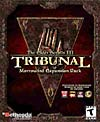
\includegraphics{media/image6.png}

{[}no fix{]} companion (is local short)

short companion

Set companion to 1

Tribunal introduced the option to "share" equipment with NPC's or
creatures. To enable this option, you must define a local short variable
named "companion" and set it to 1 or higher. Setting it to 0 or a
negative value will disable sharing. This method is used both for
mercenaries and for pack animals.

{[}no fix{]} minimumprofit (is local float)

Float minimumprofit

If ( minimumprofit \textless{} 0 )

Seems to be another variable set by the game, it is probably the
difference between current value of all goods and gold minus starting
value. If this gets negative, the mercenary can be scripted to quit.

\textbf{Sample Script:} here is the relevant part from Calvus' script
(the mercenary in Mournhold). This section handles changes in state when
Calvus leaves a contract, either because the contract expires, or
because the player has taken Calvus' stuff. The sharing is initiated
from dialogue (setting companion to 1), not in the script itself

if ( GetJournalIndex Merc\_Calvus\_Quit \textless{} 1 ) ;if Calvus has
already quit, don't do this

if ( Contract\_Calvus == 1 ) ;if Calvus doesn't have a contract, don't
do this

if ( \textbf{minimumProfit} \textless{} 0 ) ;Calvus is quitting because
player took his stuff

AiWander 128 6 0 40 30 20 0 0 0 0 0 0

\textbf{Set Companion to 0;} stop sharing

StopScript Contract\_Calvus

Set Contract\_Calvus to 0

ForceGreeting

return

else

if ( Contract\_Calvus == 0 ) ;handles Calvus after a contract expires

AiWander 128 6 0 40 30 20 0 0 0 0 0 0

\textbf{Set Companion to 0;} stop sharing

if ( GetJournalIndex Merc\_Calvus \textless{} 10 )

Journal Merc\_Calvus 10 ;first contract expired

else

Journal Merc\_Calvus 20 ; most recent contract expired

endif

endif

endif

endif

endif

{[}no fix{]} StayOutside (is local short)

short StayOutside

set StayOutside to 1

A useful variable for companions. When used in a script, it causes
whoever it's assigned to to automatically remain (and wait) outside of
any interior the player may enter (automatically rejoins upon return).
(Forum info / Grumpy)

\hypertarget{race-faction-and-rank}{%
\section{\texorpdfstring{\hfill\break
Race, Faction and
Rank}{ Race, Faction and Rank}}\label{race-faction-and-rank}}

\hypertarget{determining-race}{%
\subsection{Determining Race}\label{determining-race}}

GetRace, ``RaceID'' (returns Boolean/short)

Player-\textgreater GetRace "Dark Elf"

Returns 1 if the object is of the race indicated by RaceID.

Sample Script: This is a global script Bethesda uses to set a variable
that can be used to determine the PCs race in dialogue:

\lstinputlisting{scripts/RaceCheck.txt}

\hypertarget{determining-the-pcs-faction-status}{%
\subsection{Determining the PC's Faction
status:}\label{determining-the-pcs-faction-status}}

{[}no fix{]} GetPCRank, FactionID\_enum (returns short)

if ( GetPCRank "Telvanni" == 9 )

Returns PC's rank in faction. This will default to the Actor's faction
if FactionID is not defined. Returns 0-9 and -1 if not a member.

Sample Script: An Actor/object with the following script is only enabled
if the PC is not a member of House Redoran:

\lstinputlisting{scripts/bandenIndarysScript.txt}

{[}no fix?{]} GetPCFacRep, {[}FactionID{]} (returns short?)

This \textbf{doesn't work} in script (causes errors and/or crashes when
used).

SameFaction (returns Boolean/short)

Returns 1 if PC is in the faction of the calling object (NPC).

PCExpelled {[}"factionID"{]} (returns Boolean/short)

Returns 1 if PC has been expelled once from calling object's (NPC)
Faction, or a faction can be defined to get a specific one. For an
example script look below, PCClearExpelled function.

\hypertarget{modifying-faction-standing-and-reaction}{%
\subsection{Modifying faction standing and
reaction}\label{modifying-faction-standing-and-reaction}}

{[}no fix{]} PCJoinFaction {[}"FactionID"{]}

Makes the PC a member of the specified faction. FactionID is optional if
it is not added it will use the faction of the NPC who called the
function

LowerRank, {[}"FactionID"{]}

RaiseRank, {[}"FactionID"{]}

Raises or lowers the object's rank in its current faction. This function
doesn't work in global scripts, but works in targeted and local scripts.
It also works in dialogue. You can use the fix to raise a different
NPC's rank (NPC\_ID-\textgreater RaiseRank) in dialogue results
\textbf{only} - in scripts this function will only work on the actor the
script is attached to.

The faction ID argument is totally ignored by the game engine, so is not
required, and even if you have the faction ID as something totally
irrelevant (for example ``eel pie''), the script still compiles and runs
fine.

You cannot use RaiseRank to have an NPC join a faction (unlike the PC
version) - if the NPC doesn't already belong to a faction RaiseRank has
no effect.

{[}no fix{]} PCLowerRank, {[}"FactionID"{]}

{[}no fix{]} PCRaiseRank, {[}"FactionID"{]}

Raises or lowers the PC 1 rank in the NPCs faction. If PC is not part of
the faction, it will set the rank to 1.

\textbf{Example Script:}

\lstinputlisting{scripts/treboniusScript.txt}

{[}no fix{]} PCExpell {[}"FactionID"{]}

Expels PC from NPCs faction.

{[}no fix{]} PCClearExpelled {[}"FactionID"{]}

Clears "currently expelled" flag on the player.

Example script:

A script by Bethesda, which clears the Players expelled status after
some time:

\lstinputlisting{scripts/expelledMG.txt}

{[}no fix{]} ModPCFacRep, var\_enum, {[}"FactionID"{]}

{[}no fix{]} SetPCFacRep, var\_enum, {[}"FactionID"{]}

ModPCFacRep, 5, "Imperial Legion"

ModPCFacRep, 5, "Temple"

Modifies or defines the reaction modifier for members of the specified
faction (towards the PC).

ModFactionReaction, "factionID1", "factionID2", var\_enum

SetFactionReaction, "factionID1", "factionID2", var\_enum

Modifies or defines the reaction of one faction towards members of
another faction.

\textbf{Example}: This is part of the MoonAndStar script. This part
first makes the PC part of the faction "Nerevarine" and then sets two
factions to react particularly to this change:

;faction reaction and journal stuff

Journal "A2\_6\_Incarnate" 50

player-\textgreater modReputation 5

\textbf{PCJoinFaction}, Nerevarine

if ( GetPCRank, Redoran \textgreater= 0 )

\textbf{modFactionReaction}, "Redoran", "Nerevarine", 4

endif

if ( GetPCRank, Temple \textgreater= 0 )

\textbf{modFactionReaction}, "Temple", "Nerevarine", 4

endif

\hypertarget{determining-and-changing-reputation-and-disposition}{%
\subsubsection{Determining and changing reputation and
disposition}\label{determining-and-changing-reputation-and-disposition}}

\emph{Get/Mod/Set}Reputation

\emph{Get/Mod/Set}Disposition

SetDisposition refers to base disposition (as set in the TES CS,
unaltered by any modifiers). To set the disposition value used in game,
use a combination of GetDisposition (returns current value) and
ModDisposition; for example, to completely control an NPC's disposition
from a global "myRealDisp" (can be a short, it doesn't need to be a
float unless you want to change disposition by float values), the NPC's
local script could include something like this:

if ( myRealDisp \textgreater{} 100 )

set myRealDisp to 100

elseif ( myRealDisp \textless{} 0 )

set myRealDisp to 0

endif

set localFloatVar to ( GetDisposition )

set localFloatVar to ( myRealDisp - localFloatVar )

ModDisposition localFloatVar

\emph{\hfill\break
}

\hypertarget{werewolf-specific-functions}{%
\subsection{Werewolf-specific
functions}\label{werewolf-specific-functions}}

\hypertarget{set-the-werewolf-attributes}{%
\subsubsection{Set the werewolf
attributes}\label{set-the-werewolf-attributes}}

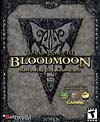
\includegraphics{media/image7.png}

SetWerewolfAcrobatics

Actor-\textgreater SetWerewolfAcrobatics

This function set the attributes of the object to those of a werewolf.
This sets the targets skills and attributes to match the fWerewolfxxxx
gameplay settings. In most cases, this means a high strength, agility,
acrobatics etc, and 0 in most other things.

Player-\textgreater AddSpell "werewolf vision"

Player-\textgreater AddSpell "werewolf regeneration"

Player-\textgreater SetWereWolfAcrobatics

\hypertarget{change-the-color-of-secunda}{%
\subsubsection{Change the color of
Secunda}\label{change-the-color-of-secunda}}

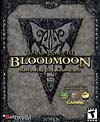
\includegraphics{media/image7.png}

{[}no fix{]} TurnMoonWhite

{[}no fix{]} TurnMoonRed

These two functions are very simple -- they change the color of Secunda
(The small, white moon) from white to red and back again. This doesn't
have any real effect to gameplay, but it does make the sky look
different. It is used during the Bloodmoon main quest -- hence the
expansion title.

if ( doOnce == 0 )

TurnMoonRed

set doOnce to 1

endif

\hypertarget{determine-how-many-kills-a-werewolf-has}{%
\subsubsection{Determine how many kills a werewolf
has}\label{determine-how-many-kills-a-werewolf-has}}

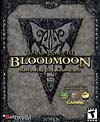
\includegraphics{media/image7.png}

{[}no fix{]} GetWerewolfKills (returns short ?)

This keeps count of how many NPC's killed by the player when in werewolf
form. Each time an NPC is killed while the PC is a werewolf, one is
added to this count. It is reset automatically when the PC changes back
into human form.

if ( GetWerewolfKills \textgreater{} 0 )

; Do code to stop the PC from being affected by the hunger.

endif

\hypertarget{check-to-see-if-the-creature-is-in-werewolf-form}{%
\subsubsection{Check to see if the creature is in werewolf
form}\label{check-to-see-if-the-creature-is-in-werewolf-form}}

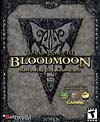
\includegraphics{media/image7.png}

IsWerewolf

If ( Actor-\textgreater IsWerewolf )

This function allows to determines if the target is a werewolf or not.
It can be used on the PC or other creatures.

if ( Player-\textgreater IsWerewolf != 1 ) ;DON'T RUN IF PLAYER ISN'T
WEREWOLF

return

endif

\hypertarget{change-to-a-werewolf}{%
\subsubsection{Change to a werewolf}\label{change-to-a-werewolf}}

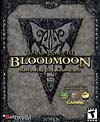
\includegraphics{media/image7.png}

BecomeWerewolf

UndoWerewolf

Actor-\textgreater BecomeWerewolf

Actor-\textgreater UndoWerewolf

These functions change the target object to a Werewolf or change them
back to their original form. IMPORTANT: Using Becomewerewolf and
Undowerewolf CAN break your game. Some quests and variables depend
solely on use of these, so if you use one to toy around.... you may be
asking for it. (This message brought to you by your friendly dev
WormGod).

Note:

When the player is a werewolf, the only thing you can detect them
activating (Using OnActivate) is doors.

If you want to detect the player activating an object, or even another
werewolf, one method is to use an invisible door and place it over the
object you want to detect the activation of.

if ( OnPCEquip == 1 )

Player-\textgreater BecomeWereWolf

Set OnPCEquip to 0

Endif

Set timer to ( timer + GetSecondsPassed )

If ( timer \textgreater{} 10 )

Player-\textgreater UndoWereWolf

Endif

\hypertarget{section-8}{%
\subsubsection{}\label{section-8}}

\hypertarget{section-9}{%
\subsubsection{}\label{section-9}}

\hypertarget{section-10}{%
\subsubsection{}\label{section-10}}

\hypertarget{special-werewolf-global-variables}{%
\subsubsection{Special werewolf global
variables}\label{special-werewolf-global-variables}}

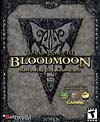
\includegraphics{media/image7.png}

{[}no fix{]} PCknownWerewolf (is short global)

A global variable that indicates whether the PC is a known werewolf

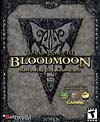
\includegraphics{media/image7.png}

{[}no fix{]} PCWerewolf (is short global)

Set to 1 when player is werewolf. Used in controlling numerous werewolf
scripts.

It works in the same way as PCVampire:

-1 = Player has been cured of lycanthropy and cannot become a werewolf
again

0 = Player is not a werewolf

1 = Player is a werewolf

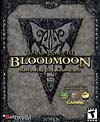
\includegraphics{media/image7.png}

{[}no fix{]} WerewolfClawMult (is float global)

A multiplier for claw damage. Exact formula unclear, see werewolf
scripts for reference.

\hypertarget{text-and-dialogue}{%
\section{\texorpdfstring{\hfill\break
Text and Dialogue}{ Text and Dialogue}}\label{text-and-dialogue}}

\hypertarget{brief-dialogue-how-to}{%
\subsection{Brief dialogue how-to}\label{brief-dialogue-how-to}}

Dialogue is an art in itself that can not be fully covered here.
However, when creating quests you will often mesh dialogue and scripting
to control your quest and achieve certain effects. Therefore, I will
give a brief introduction.

\hypertarget{the-concept-of-mw-dialogue}{%
\subsubsection{The concept of MW
dialogue}\label{the-concept-of-mw-dialogue}}

In Morrowind, dialogue is organized in a database. This database is
structured in the following way:

Top level:

The different "divisions" of dialogue are:

\emph{Topic:} The actual topic words and responses for the dialogue
window in the game.

\emph{Greetings:} The text strings you are greeted with when you
initiate dialogue with an Actor.

\emph{Persuasion:} The answers you get for successful or failed
persuasion attempts.

\emph{Journal:} The entries for your journal.

\emph{Voice:} The .mp3 sound files (and subtitles) that players "say"
when you come near, are hit, are fleeing, etc.

Find these divisions on the tabs on the top left of the dialogue window
(use the arrows to get to the hidden tabs).

Sub-level 1:

Each of these top level divisions has sublevels I call topics -- for the
\emph{Topics} division, these are the actual "keywords" (topics) that
Actors will have something to say about. These are the words that will
be highlighted ("hyperlinked") in in-game text and listed in the right
hand panel of the dialogue window. For \emph{Journal} these are the
different journals (usually one per quest). For \emph{Voices} the
different categories of sound responses that are "triggered" by the
appropriate in-game conditions etc. For \emph{Greetings} these are just
general categories of greetings (diseased, quest offers, standard and so
on). This is the way Bethesda has used them (forum info / Emma):

\begin{itemize}
\item
  Greetings 0: Npc is alarmed
\item
  Greetings 1: Quests (actually quests where it doesn't matter if the
  Player is a vampire, is nude, is a criminal, is diseased).
\item
  Greetings 2: Player is a vampire/player is nude
\item
  Greetings 3: Traitors to Morag Tong
\item
  Greetings 4: Crime and disease
\item
  Greetings 5: Quests
\item
  Greetings 6: Factions
\item
  Greetings 7: Classes, Endgame, Slaves
\item
  Greetings 8: Clothes (general greetings concerning how player is
  dressed)
\item
  Greetings 9: Locations.
\end{itemize}

For \emph{Persuasion} these are things like service refusals or bribe
success/fail messages.

Sub-level 2:

For each topic there can be one or several sub-entries ("Info/Response")
-- these are the actual responses. For \emph{Topic} and \emph{Greetings}
these are the actual answers of Actors to the topic phrase. For
\emph{Journal} these are the different entries describing the progress
of a quest.

These entries represent a linked list, meaning that each entry contains
(invisible) info on which is the next response in line and which is the
previous. (This leads to a common error message when dialogue gets
deleted or scrambled, e.g. by cleaning a mod with TESAME, or by loading
several mods that change the same topic. The game doesn't know for sure
any more which entry comes after which. This sometimes doesn't matter,
but it can also mean that certain responses are cut off, because the
order isn't right any more -- this depends on the conditions). To check
and/or change the next/previous ID strings, you can export the dialogue
and re-import it if necessary (solution suggested by Kateri).

Dialogue entries come with conditions that you can set in the dialogue
editor window. In the topic window you will find a list of general
conditions on the left -- here you can define which Actor (Actor ID) or
group of Actors (Race, Class, Disposition, etc.) potentially know this
response. There are also two conditions for the PC (PC faction and
rank). To the right you can set a maximum of 6 "free" conditions that
can refer to the Actor, the PC or other things like the state of global
variables -- lots of options here, you will have to see for yourself.
Check for journal entries, player stats, local or global variables,
items in inventory, and many other functions, some equivalent to script
functions, some unique to dialogue (see below).

An important and initially confusing feature of the dialogue editor is
the filter option (lower left-hand corner). When you select an Actor ID
here, you only see the topics that this Actor can possibly know (as
described above). Remember that when you create a \textbf{new} topic
(maybe specifically for that NPC) it contains no responses. Thus the
Actor cannot "know" it and thus the freshly created topic does not
appear! Select the empty slot on the very top to see all topics again,
make a response for the new topic that your Actor can "know" -- then you
can turn the filter on again, if you wish.

\hypertarget{how-dialogue-works}{%
\subsubsection{How dialogue works}\label{how-dialogue-works}}

To decide whether a dialogue \textbf{topic} is available during dialogue
with an NPC, the game checks:

\begin{enumerate}
\def\labelenumi{\arabic{enumi}.}
\item
  Whether the NPC "knows" the topic -- this is determined by the
  conditions set in the "speaker conditions" field -- if the NPC can
  fulfill the conditions for just one of the responses for that topic,
  he "knows" it.
\item
  Whether the Player knows it. The PC knows a topic if it (the topic
  word) either appeared previously in a response from an NPC or if it
  was specifically added with the AddTopic function. Note that the
  addition of a topic to the list of topics the PC knows only happens if
  the keyword becomes available in the same NPC's dialog that says the
  topic keyword. An example: let's say you try to trade with a weapon
  merchant and he denies you service because you have skooma in
  inventory. The word "skooma" is used in the dialogue, and there is a
  topic "skooma", but it is not familiar to weapon merchants. After
  that, you talk to a savant who \emph{is} familiar with the topic...
  but you are still not. The topic will appear in your list only when he
  (or someone else familiar with it) will mention skooma in one of
  responses (Forum info / Kir).
\item
  If both the PC and the Actor "know" the topic it shows up in the topic
  list and gets highlighted in the text -- it can now be selected by the
  player and an appropriate response will be given.
\end{enumerate}

When the game has to select the correct response from the list of
responses for that topic, it does the following:

\begin{itemize}
\item
  It starts checking \textbf{from the top} of the list, whether the
  conditions for that response are met, which means \textbf{all}
  conditions that have been defined for that response return "true".
\item
  If not -\textgreater{} Game moves on to the next item in the list and
  checks again.
\item
  If yes -\textgreater{} this entry is used and printed to the dialogue
  window.
\end{itemize}

Special rule for greetings: if none of the items in the list are met,
move on to the next level 1 item (e.g. if no greeting in "Greeting 0"
returns true, start checking "Greeting 1".

Special rule for Journal: there is only one condition here, the index
(called by Journal function). It must be exactly met.

Once a response has been selected, the game will

\begin{itemize}
\item
  Output the text string to the dialogue window (or play the mp3 for
  \emph{Voice} responses)
\item
  Execute any Script commands in the Results field (at the very bottom).
  You can use all scripting functions here. Conditions (\emph{if}
  command) can also be used (Thanks to Kir and Manauser for this info).
  Nested ifs are possible with Bloodmoon, not sure about earlier
  versions.
\end{itemize}

Be aware that the result field allows you to exchange information with
scripts (e.g. by setting variables or adding journal entries) and that
scripts can vice versa influence dialogue as well, by setting conditions
that can be tested (e.g. you can check for local or global variables in
the speaker conditions of dialogue). The simplest script that influences
dialogue is the nolore script, which is just used as a flag to keep
Actors from using standard dialogue.

\textbf{Note:} Result field scripts are not compiled by CS. You may
write any rubbish there and MW will not complain until the line is told
by an NPC and its script is compiled on-the-fly. If the script is
complex enough to worry about possible syntax errors, it is recommended
to copy/paste its text into a regular dummy script and try to save it.
That is more reliable than using the "Error Test Results" button, as it
can change preset values of global variables. On the other hand, the
fact that resultbox scripts are compiled at runtime may allow some
interesting effects, like addressing contents of another mod without
duplicating it in the current mod, which can't be done with conventional
scripts (Forum info / Kir).

\hypertarget{creating-clean-dialogue}{%
\subsubsection{Creating clean dialogue}\label{creating-clean-dialogue}}

\emph{(Thanks to JOG and Cyran0 for this information)}

\emph{When you are adding dialogue to an existing topic (including
Greetings, Voices, etc):}

\begin{itemize}
\item
  Be very careful in using a copy/edit based method. \textbf{Never}
  change an original line: only edit the copy (top line of the two).
  Editing the copy is safe, but the two may be easily confused.
\item
  \textbf{It is preferable to "clean" the original dialogue lines
  (infos) on either side of the inserted dialogue.} This can be done in
  "Details" view by toggling the "ignore" flag for the changes, or by
  using a third-party tool, as outlined in the 'Cleaning up your mod'
  section.
\item
  It is strongly recommended that you use only one insertion point
  wherever possible (you can usually achieve this by duplicating the
  text of original lines in new locations if need be).
\item
  If you are removing \textbf{all} entries you have added to a topic, or
  cleaning original dialogue of changes: use the details view, TESAME or
  a similar utility that will \emph{remove your changes}.
\item
  If you are removing one or more lines you have added (but not all
  lines in a block), do not simply clean the changes. In order to ensure
  the info-IDs are updated correctly, you should \emph{delete the
  line(s)} in the dialogue editor itself (right-click and delete, or
  'delete' key when line is selected). The editor will update the IDs
  automatically. (If for some reason you cannot do this, you can move
  the dialogue line to be deleted as far away from all other new
  dialogue as is possible, then use ignore: moving the info will also
  update IDs automatically, and the original dialogue modified by the
  move may be cleaned as above. Alternatively, you can export the
  dialogue, edit as necessary and re-import it.)
\end{itemize}

\hypertarget{some-explanation}{%
\subparagraph{Some explanation:}\label{some-explanation}}

Dialogue is a linked list: each info contains its own ID-string, and the
IDs of the previous and next lines. You can see this more easily by
exporting the dialogue and viewing it in a text editor: the long numbers
are the IDs, and the pattern should be obvious.

When you change an original line, the ID-string stays the same: this has
a similar effect to the one modders are familiar with in different mods
changing the same thing, or adding objects with identical IDs\ldots{}
\emph{The last mod to load wins}. The text and conditions of the last
mod to load will overwrite the text and conditions in other mods,
dialogue from mods that load earlier and contain that line may lose its
place, and some entries may be shifted to new (and usually highly
problematic) positions in the list. (New entries themselves are highly
unlikely to be subject to the same problem, as 'copy' or 'new' creates a
new, randomly-generated ID for the new dialogue line: note that 'copy'
does not copy the ID, it generates a new one. However, if you were to
copy an .esp with dialogue, e.g. in order to reuse the dialogue for a
different NPC, the dialogue would still have the same info-IDs as in the
original mod and the two mods would be incompatible. This still applies
if you change the topic IDs: you need to change the info-IDs as well!)

When you add dialogue to an existing topic, this in itself modifies the
original dialogue around it as the CS updates the next/previous info-IDs
to point to the new line. That changed original line can overwrite (or
be overwritten by) the same line - \emph{including its links to the
next/previous lines} - in other mods when the game loads, causing
dialogue lines to lose their place and be moved.

The way to avoid this (as much as is possible) is to clean the changes
from the original dialogue. This will give errors when the mod is loaded
in the CS ("previous/next string is different than expected for
ID\ldots" kind of errors)\ldots{} but since the new dialogue lines still
have the correct previous/next IDs the dialogue will (if all mods are
clean) be correctly placed when loaded in either the CS or the game, and
since the original dialogue is not changed it will not overwrite
original lines for other mods. Problems can still arise in some
circumstances, most particularly if an "unclean" mod loads later, but
most modders will already be familiar with this problem in other areas
(object property editing, for example, can be similar).

One problem which can arise with this method is that if your dialogue
uses more than one insertion point, so that an original line has new
dialogue both directly above and directly below, cleaning it will cause
problems. The safer method is to simply copy the original line and use
the copy, leaving the original below all your dialogue (and therefore
unused by the game) - thus keeping a single insertion point.

\emph{Further notes:}

Another point which I think fits the spirit if not quite the letter of
'creating clean dialogue' is this: It is not advisable (or, perhaps, not
\emph{polite}) to put your more generic dialogue higher in the chain
than it needs to be, nor to filter any of your dialogue more broadly
than necessary. This just leads to a game of one-upmanship as modders
try to get their dialogue higher to prevent other mods breaking it.

If possible, avoid adding dialogue that will be used by existing NPCs
(those not added by your mod) - and be especially careful of this in
Greetings. It is often suggested that you use filters unique to your mod
when creating new dialogue that is not filtered for actor ID, e.g. new
factions, classes, or cells. While this is good advice in general, be
aware that unless you prevent it, many players are likely to bring
companions into your new cells - and those companions will have any
dialogue that is filtered solely for that cell (usually not a desirable
outcome). If possible, you may want add a nolore filter to prevent this
(preferable to using the companion variable as some still use
Morrowind-only companions, and almost all companions and other followers
are nolore'd - but "not local companion \textgreater= 0" will still rule
out the vast majority of companions). You can also filter dialogue for
an otherwise-unrelated selection of NPCs from your own mod by using a
uniquely-named local variable as a filter (but all those NPCs will need
to have local scripts for this to work).

\hypertarget{a-few-golden-rules}{%
\subsubsection{A few golden rules}\label{a-few-golden-rules}}

\begin{itemize}
\item
  \textbf{The most specific responses should be on top of the list, the
  "catch all" answers should be lowest!} Remember the first one that
  returns true is the one that gets picked. So you can't have a response
  for everyone in Vivec above one for a specific NPC in Vivec.
\item
  \textbf{If you want an NPC to be able to talk with the PC about
  something special, you must introduce the topic word, e.g. in a
  greeting or in a "latest rumors" response.} Alternatively, you can use
  a script with the AddTopic function.
\item
  \textbf{Don't use normal words as journal topics.} Topic, Greeting,
  Journal are actually all in the same database -- that's why journal
  topics use a format like A1\_dreams. If it were just "dreams" than the
  journal entry to "dreams" could come up as a dialogue response to the
  word "dreams".
\item
  \textbf{Never delete a topic that belongs to the original Bethesda
  master files.} This is very hard to repair and will cause severe
  errors in peoples save games. (Emma). You should also avoid deleting
  responses from the original game: the best way to remove a response is
  simply to add your custom dialogue above the original response, so it
  still exists unchanged but is never "said"; if this is not possible,
  you can change the filtering for the response (e.g. filter for ID
  "dialog placeholder" will remove the response from all NPCs in the
  game world) - but changes to an original response will be overwritten
  by any later-loading mod that also changes that response.
\item
  \textbf{If you are using the greetings section 1, don't put your
  greetings at the very top of it.} The top greeting belongs to a
  certain quest, and must be left at the very top in order to always
  show up. You can put your greetings below these instead. (Emma)
\item
  If at all possible, avoid putting your new responses as the very first
  or very last entry in an existing topic (this includes greetings). For
  example, if you want your greeting to be above the first greeting in
  Greeting 2, put it in Greeting 1. If you want it below the last
  greeting in Greeting 1 as well, then copy that greeting and put the
  copy above your new greeting: this will achieve the same effect, as
  the original line will never be "said".
\end{itemize}

\hypertarget{dialogue-101}{%
\subsubsection{Dialogue 101}\label{dialogue-101}}

The following summarizes some of the most frequent problems with
dialogue. This list was assembled from a forum discussion with
contributions by Klinn, Emma and GarryB.

Tip 1) \textbf{My new topics disappear!} Go to the Filter box at the
bottom of the list of topics. Clear the filter by choosing the top empty
line in the drop-down list. Recommend using the button on main toolbar
to bring up the dialogue editor rather than from the NPC's properties
(if you open the dialogue window from an NPC's property box, it will be
filtered for that NPC by default; but if you open the window from the
main toolbar or menu, it will be unfiltered by default).

Tip 2) \textbf{My NPC keeps asking me a question over and over!} Be sure
to put the replies \emph{above} the original question. Sounds backwards,
but it works.

Tip 3) \textbf{My NPC talks about everything!} To keep an NPC from
having the standard topics about Morrowind lore, attach the script
"NoLore" to him or her. If you already have a script on the NPC, add the
declaration \textbf{Short NoLore} near the top.

Tip 4) \textbf{My NPC still has extra topics!} Some other general topics
may appear depending on an NPC's faction or class. For example, members
of the Imperial Legion will always automatically have topics about that
faction, the Empire, and more. There are some lore topics that are not
well-filtered and will appear in certain circumstances regardless
(especially with Bloodmoon: many BM NPCs are NoLored to avoid
\emph{Morrowind} lore topics, and most Bloodmoon lore topics are
filtered only for cell). If this is a real problem, and your mod design
allows for it, you can use a creature instead of an NPC: creatures can
only have dialogue filtered for specific ID.

Tip 5) \textbf{How do I add topics for just my NPC?} After creating the
topic and it's Info/Responses, in the Speaker Conditions area, set the
ID to your NPC.

Tip 6) \textbf{I added topics but my NPC doesn't have them!} Two
possibilities: the PC must have already heard (read) that topic word or
phrase before he can ask about it. Usually this is done by having the an
NPC's greeting include the topic. Second possibility: there may be
Speaker Conditions that prevent the topic from appearing. Even if it
appears when you filter the dialogue for an NPC, some topics depend on
the player having reached a certain point in the game, having a specific
journal entry, and so on. Note that since the resultbox scripts are
executed \emph{after} the display has updated, a topic made available by
a resultbox script may not appear immediately. Another little trap is
that topics won't be added and hyperlinked in dialogue if they don't
begin with a letter, so topics like "-follow" won't be hyperlinked in a
greeting even if the conditions are met: you will need to use AddTopic.

Tip 7) \textbf{How do I change the order of my Responses?} Use the
left-arrow and right-arrow keys to move an Info/Response up or down in
the list. Note that every original entry that is "touched" by your moved
dialogue will be marked as changed: you can remove your changes using
the details view.

Tip 8) \textbf{How do I create dialogue for creatures?} Any creature can
have its specific dialog. You do this exactly as you create the dialog
for an npc, with one difference.

You have to have the dialog UNFILTERED when making the dialog (i.e. the
slot below the topics must be empty). Once you have created the dialog
lines, you can filter them for your creature. \emph{Note: This is
because creatures can only have dialogue that is filtered for specific
ID, and when you create a new response it isn't filtered at all - so the
creature can't "know" it.}

Tip 9) \textbf{What are typical uses for the dialogue result box?} Emma
lists these useful and frequently used commands for the result box:

\begin{itemize}
\item
  Player-\textgreater AddItem "my item" 1 (a specific item is added to
  players inventory)
\item
  Player-\textgreater RemoveItem "my item" 1 (a specific item is removed
  from players inventory)
\item
  ModDisposition 5 (npc will like player 5 points better)
\item
  cast "my\_new\_spell" player (the npc will cast a certain spell)
\item
  AiFollow Player 0 0 0 0 (npc will start follow player)
\item
  AiWander 0 0 0 0 0 0 0 0 0 0 0 0 (npc will quit following the player)
\item
  SetFight 100 (npc will start attacking the player)
\item
  StartCombat player (npc will start attacking the player)
\item
  StopCombat (yep, you've guessed it. Stop combat)
\item
  StartScript "my\_global\_script" (start a certain script)
\item
  Set companion to 1 (if you have added a "short companion" command to
  your script, this will make the npc share with you; requires Tribunal
  or Bloodmoon)
\item
  SetHealth 100 (will set the npc's health to 100 - same command can be
  used for setting other skills and attributes as well, i.e. SetMagicka,
  SetLongBlade etc.)
\item
  disable (will make the npc instantly disappear)
\item
  goodbye (will force the player to end the conversation. Can be useful
  for instance in order to avoid further small talk with a npc that has
  already been disabled )
\end{itemize}

Tip 10) \textbf{I have created so much dialogue, how can I possibly
spell-check it?} Checking spelling and grammar can be streamlined by
using the export and import functions in the Construction Set. Export
"new" dialogue to a file, use your favorite editor for automatic
spellchecking and corrections and import the corrected dialogue . Much
easier on the brain than jumping around in a myriad of topics, greetings
and journal entries. (Forum info / GarryB)

\hypertarget{dialogue-related-functions}{%
\subsection{Dialogue-related
functions}\label{dialogue-related-functions}}

Many of the following functions are not only used in scripts, but also
in the result field of the dialogue editor window.

\hypertarget{displaying-messages}{%
\subsubsection{Displaying messages}\label{displaying-messages}}

{[}no fix{]} MessageBox, ``Message'', {[}var1{]}, {[}var2{]},
{[}``button1''{]}, {[}``button2''{]}

The \emph{MessageBox} command lets you give out information to the
player. Normally these appear as a small box with the text on the bottom
of the screen that stays there for a few seconds or until the player has
clicked a button if the message box has buttons. There is a limit of 9
buttons per message box. If a dialogue window is open, \emph{MessageBox}
will output to the dialogue window! This will be in a different color so
it's a good way to show that text isn't part of dialog. For example,
"Okay I'll take the curse off. \emph{He takes the curse off}."
\emph{MessageBox} has several different modes of operation. The simplest
one is just giving out an onscreen message that appears on the bottom of
the screen for a few seconds, as in the following script that gives out
a message when the item it's attached to is equipped:

\lstinputlisting{scripts/informplayer.txt}

The second mode of operation makes the message stay on the screen until
the player presses a button:

MessageBox, "Ulyah lifts her hands and speaks the formula. You will now
be transported to Sheogorad", "ok"

In the third mode of operation you can use the messagebox to demand a
decision from the player via a message box with buttons and the
\emph{GetButtonPressed} function.

\textbf{Warning:} The use of more than one messagebox in a frame can
cause a CTD. This also includes the ``Your journal has been updated''
messagebox.

Multiple MessageBox commands in the same frame can cause a crash. The
problem doesn't seem to appear if you do 2 MessageBox commands in a row,
but stick any other commands between them and you'll have problems.
Using 3 simple messages in a row can work, but usually crashes if there
are variable substitutions involved.\\
I'm guessing it's partially an interaction with the voice subtitle
boxes. There may be some overall limit to the number of messages per
frame. -(CDCooley)

Notes by DinkumThinkum:

1. My impression is that any type of text messages have the potential
for triggering a crash if they're generated in the same frame.\\
2. The bug doesn't trigger a CTD every single time you generate two text
messages in the same frame: it appears to be a random chance of it
happening. But, from what I saw when I tested this: if you keep
generating two or more text messages in the same frame (with some other
code in between them), sooner or later you \emph{will} crash. Sometimes
my test script would cause a CTD within a few seconds, sometimes it
would take five, ten, or more minutes, but it would invariably crash if
I waited long enough.\\
3. For a start-up script I was working on when I ran into this, adding a
one frame delay between popping up a Message Box message and updating
the player's Journal eliminated intermittent start-up CTDs I had been
getting.

There also appears to be a problem if you call too many message boxes
from the same script, even if you set up a frame counter. I'm not sure
the limit, but I discovered it when testing NecroRise a while ago...
Apparently, 50 is too much. (Forum info / Cid88)

\textbf{Note:} If you use a Tribunal start script to give out a message
box with a button as soon as the game is loaded, you should delay the
MessageBox, otherwise the mouse pointer will not be displayed.

A one frame delay isn't enough if you have a massive start-up script
that runs as soon as the game is loaded. So you might want to delay
Message Boxes (that have buttons) for a second or so after the game is
loaded, just to be on the safe side. (Forum info / DinkumThinkum).

If there is already a messagebox with choices on the screen, opening
another choice messagebox will cause the first choice messagebox to
vanish. However, when the player picks on of the choices, the messagebox
vanishes and the crosshair appears but the player can't move.

Using menutest, 0 will allow the player to move again.

You can enter carriage returns to message boxes, but it requires
hex-editing the .esp. Put some unusual characters like \textbar\textbar,
then save the esp. Then hex edit the \textbar\textbar{} characters and
make them 0D0A (hex for carriage return). (Forum info / qarl)

{[}no fix{]} GetButtonPressed (returns short)

Pressed button if a message box with buttons is used, starting at 0.
Will return --1 until button is pressed.

Sample Script:

\lstinputlisting{scripts/choices.txt}

\hypertarget{displaying-variables-and-text-defines-in-a-message-box}{%
\subsubsection{Displaying variables and text defines in a message
box}\label{displaying-variables-and-text-defines-in-a-message-box}}

To display variables in a message box you need to use a syntax
describing the format of the number to be displayed. ATTENTION -- there
is a lot of wrong info in the original helpfile on this!

MessageBox "You have \%.0f days left", days\_left

The \% symbol indicates the variable. The number after the dot
determines the number of digits displayed. "f" signifies a float
variable. The helpfile lists several types (f for float, D for short or
long and S for string variables), of these I could only get f to work.
However \%g and \%G work fine for short and long variables (thanks Niyt
Owl). You can use things like \%.3g, but the digit designation will
simply be ignored. The designators are not really specific to the
variable type, \%.3f will also display a short or long variable. There
is a limit of 9 variables that can be displayed in the same messagebox
(though for some reason the error message for exceeding this limit is
"Max variables of 10 exceeded on line XXX").

String variables are mentioned in the helpfile but are to my knowledge
not implemented, you can however use dialogue text defines in message
boxes but do NOT use \%: for text defines --In scripts it's \^{}instead
(thanks Ragnar\_GD):

Text defines:

\^{}PCName The player's name.

\^{}PCClass The player's class.

\^{}PCRace The player's race.

\^{}PCRank The player's rank in the speaker's faction.

\^{}NextPCRank The player's next rank in the speaker's faction.

\^{}Cell The cell the player is currently in.

\^{}Global Any global variable value. Floats display as 1.1, such as
\^{}Gamehour

\textbf{Note:} you can also display a Global variable normally, using
the above syntax such as \%.1f, which would yield the same result. If
you use the \^{}Global text define in a book, Morrowind will usually
crash if you access or change the global variable while the book is
open. This should be avoided at all costs! (Forum Info/Chris\_K)

\^{}Name The speaker's name.

\^{}Race The speaker's race.

\^{}Class The speaker's class.

\^{}Faction The speaker's faction. If they have no faction, it will be
blank.

\^{}Rank The speaker's rank.

\textbf{Note:} These last listed ones will not work quite as they do in
dialogue, as the defines default to the PC's values by default, not to
the calling Actor. So \^{}Name and \^{}PCName will both display the PC's
name, even if the MessageBox is called from dialogue results.

\hypertarget{example-script-stupid-sample-script-demonstrating-all-possible-syntax}{%
\subparagraph{Example Script: Stupid sample script demonstrating all
possible
syntax:}\label{example-script-stupid-sample-script-demonstrating-all-possible-syntax}}

% Bug here

\lstinputlisting{scripts/test1.txt}

\hypertarget{adding-a-dialogue-topic}{%
\subsubsection{Adding a dialogue topic}\label{adding-a-dialogue-topic}}

{[}no fix{]} AddTopic, "Topic"

AddTopic, "Topic"

Once you have set up a dialogue topic in the TESCS, you may find that
you still can't talk about it with the NPC you have given the dialogue
to, because for the game you don't know that particular topic yet. There
are two ways to change that condition: either you introduce the topic in
another conversation topic (e.g. a custom greeting) or you give it to
the player via script, which makes sense when it's an obvious topic the
player would ask about without being brought to it by conversation (e.g.
if you see and NPC standing under a waterfall, you might want to ask him
about "aren't you getting wet?" even if the NPC doesn't bring up the
topic.

To do that, just attach a small script to the NPC:

\lstinputlisting{scripts/AddSpecialDialogue.txt}

\textbf{Note:} You must already have the topic with this topic ID set up
before you make this script, otherwise the script compiler will
complain.

Even if a topic is introduced through dialogue, it may also be useful to
use AddTopic in the resultbox of the line that introduces the topic. If
another mod adds a topic with the same ID or an ID of which your topic's
ID is a subset, your topic may not be hyperlinked, but AddTopic will
ensure that it appears in the speaker's topics list anyway.

AddTopic adds the topic to the \textbf{player's} "known topics" list. So
using\\
"Actor\_ID"-\textgreater AddTopic "blabla" is wrong: an NPC's known
topics are entirely predefined by speaker conditions.

You can not remove a topic via script; you can however set a speaker
condition in the Dialogue editor which can be set from script (e.g. a
variable or journal entry), which can be used to achieve the same
effect.

\hypertarget{initiating-and-ending-dialogue}{%
\subsubsection{Initiating and ending
dialogue}\label{initiating-and-ending-dialogue}}

ForceGreeting

ForceGreeting can be used to make Actors initiate dialogue. When
\emph{ForceGreeting} is called the dialogue window will open, and the
Actor will use a greeting according to his dialogue settings. Therefore,
if you want a special greeting by the Actor, you have to provide it via
the dialogue window in the TES CS. It does not matter where the NPC is,
this function will always work, so its usually best used in connection
with a \emph{GetDistance} or \emph{GetPCCell} condition.

Note that ForceGreeting will \textbf{not} work remotely if the player
has not encountered the NPC in the last 72 game hours, \textbf{unless}
the NPC has "corpses persist" checked (in which case it will work as
long as the player has encountered the NPC at some point during the
game). This also applies to the "Talked to PC" flag. -(Forum info/Neko)

An alternative workaround: If you use PositionCell on the NPC once per
day (even without changing their location), the 72 hour time limit no
longer applies (Forum info /Time limit info from Cortex, thanks to
Srikandi for bringing it to my attention). This trick to get around
Actors breaking their connection to you after 72 hours seems to require
the cell you send them to to not be the cell where you initially met
them (Forum info / Cortex). This either implies it must not be their
editor starting cell or that it must be a cell that you have not
visited. In my fix I have an interior I send them to for this purpose so
either explanation could be why it works. So basically after you have
met them they get sent there each day even though they are already there
after the first sending.

See the "72-hours bug" section under "Tips and Tricks" for more
information.

Using ForceGreeting \emph{in dialogue results for a greeting} can be a
useful trick in some circumstances, usually to have a resultbox script
executed without providing extra, unique text for it (you can just use a
dot "." as the text). The NPC will then give whatever greeting would
normally be given, with just an easily-ignored dot above as evidence
that your resultbox script was executed. \emph{Note that you
\textbf{must} change the tested conditions in the resultbox script -
otherwise it will loop continuously and crash the game!}

Note also that if an NPC's "Talked to PC" flag is set by your "fake"
greeting, any normal greetings that rely on it won't be given. If this
is an issue, you could filter your fake greeting for "Talked to PC != 0"
to avoid this (the player will then have to talk to the NPC a second
time before your script runs).

\textbf{Example Script:} this script shows a nice set of condition being
checked before initiating the \emph{ForceGreeting} command

\lstinputlisting{scripts/balynScript.txt}

\textbf{Note:} If you use ForceGreeting from within an if block, the
script will continue to execute the remaining elseif/else tests instead
of skipping over them (as it should). To avoid this, add a \emph{return}
after the ForceGreeting.

This script will print the messagebox:

if ( ( Actor\_ID-\textgreater GetDisposition ) \textgreater= 80 )

Actor\_ID-\textgreater{}\textbf{ForceGreeting}

else

MessageBox "I'm not talking to you!"

endif

Here is the corrected version:

if ( ( Actor\_ID-\textgreater GetDisposition ) \textgreater= 80 )

Actor\_ID-\textgreater{}\textbf{ForceGreeting~}

\textbf{return}

else

MessageBox "I'm not talking to you!"

endif

Goodbye

\emph{Goodbye} forces the end of dialogue: after calling this function
the PC can only choose the goodbye option and thus close the dialogue
window. Usually this function is used in the result section of a
dialogue topic, not in scripts; however, it can be used in scripts if
the dialogue window is open.

\hypertarget{allowing-forced-dialogue-with-werewolf-player-bloodmoon}{%
\subsubsection{Allowing forced Dialogue with Werewolf player
(Bloodmoon)}\label{allowing-forced-dialogue-with-werewolf-player-bloodmoon}}

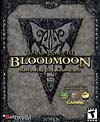
\includegraphics{media/image7.png}

{[}no fix{]} AllowWereWolfForceGreeting (is short variable)

Short AllowWereWolfForceGreeting

This variable allows to use ForceGreeting on a werewolf character. Used
on cariushuntscript, dulkscript, heartfanghuntscript. The variable
simply has to be declared, not set to a specific value.

\textbf{Example:}

\lstinputlisting{scripts/dulkScript.txt}

\hypertarget{multiple-choice-asking-questions}{%
\subsubsection{Multiple choice -- asking
questions}\label{multiple-choice-asking-questions}}

{[}no fix{]} Choice, ``choice 1'', choice1\_enum {[}"choice 2",
choice2\_enum, \ldots{]}

Choice "yes", 1, "No, certainly not!", 2

This is used in dialogue result fields to ask a decision of the player
or can be called just to "continue" a longer speech. After the PC makes
his choice, the same topic will be checked again, and you can provide
the correct response by using function / choice / = / choice\_enum in
the speaker conditions of the dialogue window. Choice can be used in
script, if the dialogue window is open. If the same resultbox/script
contains more than one choice call, the choices are presented to the
player as a single list (unlike MessageBoxes).

\hypertarget{section-11}{%
\subparagraph{}\label{section-11}}

The limit of choices per result or per call may well be version
dependent. It has been reported that there is a limit of 5 choices per
call, but I'm not sure which version this was tested with. Under version
1.6.1820, I don't think there's a limit on the number of choice
\emph{calls} in a single result, but only 20 choices can be displayed on
screen at one time: if more are displayed, the game will freeze when the
player clicks one (this applies to scripts as well as dialogue results).
More than 20 \emph{possible} choices won't cause problems as long as no
more than 20 are actually displayed (i.e. using conditional statements
to select 20 or less from a larger number of choices is OK).

On using Choice in script: I don't advise using it in a script that also
contains a StartScript command, as this can also freeze the game
sometimes. If you need to use both, you might try delaying the
StartScript part until out of menumode if possible or using some
condition to ensure that the choices can't be given more than once (not
tested).

\hypertarget{adding-to-the-journal-and-testing-journal-entries}{%
\subsubsection{Adding to the journal and testing journal
entries}\label{adding-to-the-journal-and-testing-journal-entries}}

{[}no fix{]} Journal, "Journal\_ID", Index\_enum

Journal, MG\_BCShroomsCombat, 10

This adds a journal entry to your in-game journal. The journal entry
must have previously been set up in the dialogue editor. Index
references which part of a journal topic is added. Beware of using
simple names for journal topics, adhere to Bethsoft's two letter
standard (see above example) -- otherwise the journal entry might show
up as a regular conversation response, just like any other, if the topic
title shows up in a conversation!

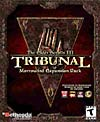
\includegraphics{media/image6.png}

{[}no fix{]} SetJournalIndex "Journal\_ID" index\_enum

SetJournalIndex "MG\_BCShroomsCombat" 99

SetJournalIndex will set the index to the specified value, whether or
not an entry exists for that index. This can be used to restart quests
or repeat sections (by setting the index backwards), or for temporary
storage of simple flags that don't need an own journal entry. However,
it should not be used to finish quests, as the quest will not be removed
from the active quests list (Journal does not have this problem, so it
is to be preferred for finishing quests).

\textbf{Note:} If the index set does not have a valid journal entry
(i.e. that index isn't defined in the "info" section of the dialogue
window), the value will be lost when a savegame is reloaded (the index
will revert to the last valid entry given). Therefore this can also be
used to detect if the player has reloaded the game:

if ( ( getjournalindex "dummy" ) != 100 )\\
Messagebox "You just reloaded, Cheater!!!"\\
setjournalindex "dummy" 100\\
endif

Where "dummy" is any journal topic that has no text for index 100.\\
\strut \\
The best thing is that it's most easy to use this in dialogue: Send the
player to the "test of courage", and set the journal index in
dialogue-result. When the player comes back, and the index differs, then
the player has failed the test. (Info on this function provided by JOG).

{[}no fix{]} ClearInfoActor

This is a function that is used in the results section of a dialogue
response -- using this function will stop the response from appearing in
the PC's journal (under "Topics"). Useful to avoid cluttering the topic
with useless information. Note however that if all responses for a topic
use ClearInfoActor, the topic will still appear in the topics list in
the journal, but clicking it will take the player to a blank page.

{[}no fix{]} GetJournalIndex, "JournalID" (returns short)

If ( GetJournalIndex, MG\_BCShroomsCombat == 10 )

This function returns the index of the current journal entry for that
journal topic (meaning the last index given, or the last index given for
which an entry exists in the case of SetJournalIndex and a reloaded
savegame). This is very convenient for keeping track of quest
advancement, and to have a script react according to what parts of the
quest have already been performed.

Sample Script: Here is a short script demonstrating the use of both
functions from the game:

\lstinputlisting{scripts/attack_slave.txt}

\hypertarget{special-dialogue-only-functions}{%
\subsubsection{Special dialogue-only
functions}\label{special-dialogue-only-functions}}

Among the functions available for defining dialogue conditions in the
dialogue editor there are a few that do not have a direct equivalent in
scripting functions. By using dialogue (e.g. using ForceGreeting,
voice-dialogue or strategically placed quest NPCs) and the dialogue
result field, you can still make use of these functions for scripting
purposes, e.g. by setting a global variable in the result field.
Examples of such functions are:

PC Sex (dialog)

This is 0 if the player is male and 1 if the player is female.

\textbf{Note:} This is the only known way to determine the player's sex.
You could use this to set a global variable that contains the Player's
gender - the most inconspicuous way would be to do this via voice
dialogue, e.g. one could put a silent hello greeting for all NPC's on
top of the list that sets a global variable "PC\_sex" to 1 when the
player is female, 2 when the player is male. The topic should be
filtered to only be active when PC\_sex equals 0.

Talked to PC (dialog)

This is 1 if the speaker has talked to the player and 0 otherwise. You
can use this to have someone say something the first time you speak with
them -- or for our scripting purposes to mark this person as "known" by
the player.

\textbf{Note:} The Talked to PC flag is subject to the "72-hours bug",
i.e. it will by default be reset if the NPC's cell has not been active
for 72 game hours or longer. See \emph{ForceGreeting} for specific
workarounds, and the "72-hours bug" section under "Tips and Tricks" for
more general information.

Rank Requirement (dialog)

Rank Requirement checks to see if you "qualify" for the next rank in the
speaker's faction.

\begin{itemize}
\item
  Returns 0 if you do not have enough Faction Reputation and do not meet
  the skill requirements.
\item
  Returns 1 if you meet the skill requirements, but do not have the
  Faction Reputation.
\item
  Returns 2 if you have the Faction Reputation, but do not meet the
  skill requirements.
\item
  Returns 3 if you qualify.
\end{itemize}

PC Clothing Modifier (dialog)

This is the total value of all the clothing and armor the player is
wearing. The value of your equipment changes the disposition of people
in the game.

Friend Hit (dialogue)

Used in dialogue for when you attack a member of your group (like a
follower)

The return values are:

0 = never been hit

1 = hit by pc 1st time

2 = hit by pc 2nd time

3 = hit by pc 3rd time

4 = hit by pc 4th time and the npc/creature is not in combat with the PC

Friend hit will reset if the player hits a different actor. It also
appears to reset if the actor starts combat, even if there are no hits
(I tried "ActorID-\textgreater StartCombat ActorID" - i.e. "start combat
with yourself" - in dialogue results, and this seemed to reset friend
hit).

\hypertarget{changing-the-hello-setting}{%
\subsubsection{Changing the Hello
setting}\label{changing-the-hello-setting}}

Get/Mod/SetHello

Changing this changes it for ALL references of the Actor. Some info from
the helpfile: Hello equates to the distance at which the Actor will
stop, face the PC and say hello. The setting (which defaults to 30) is
multiplied by the game setting, iGreetDistanceMultiplier, which defaults
to 7. Thus, a setting of 30 yields a hello distance of 210 (just under
10 feet).

\hypertarget{useful-dialogue-variables}{%
\subsubsection{Useful dialogue
variables}\label{useful-dialogue-variables}}

A number of short variables are used by Bethesda to block certain
dialogue. These must simply be declared in a script on the actor, no
value is required.

They are checked for using the Not Local filter as described in the
helpfile:

\begin{longtable}[]{@{}
  >{\raggedright\arraybackslash}p{(\columnwidth - 2\tabcolsep) * \real{0.14}}
  >{\raggedright\arraybackslash}p{(\columnwidth - 2\tabcolsep) * \real{0.86}}@{}}
\toprule
\begin{minipage}[b]{\linewidth}\raggedright
Nolore
\end{minipage} & \begin{minipage}[b]{\linewidth}\raggedright
Blocks most non-specific dialogue
\end{minipage} \\
\midrule
\endhead
NoIdle & Blocks Idle voice, used for vampires \\
NoFlee & Blocks flee voice, used for vampires \\
NoHello & Blocks Hello voice, used for vampires \\
\bottomrule
\end{longtable}

This is true if the speaker does not have this local variable. Unlike
most "Not" functions, this one does care what you set the variable to.
Both the dialogue and the variable itself should be set to 0. This can
be confusing. Here is a table of how this works:

\begin{longtable}[]{@{}
  >{\raggedright\arraybackslash}p{(\columnwidth - 6\tabcolsep) * \real{0.25}}
  >{\raggedright\arraybackslash}p{(\columnwidth - 6\tabcolsep) * \real{0.25}}
  >{\raggedright\arraybackslash}p{(\columnwidth - 6\tabcolsep) * \real{0.25}}
  >{\raggedright\arraybackslash}p{(\columnwidth - 6\tabcolsep) * \real{0.25}}@{}}
\toprule
\begin{minipage}[b]{\linewidth}\raggedright
Not Local
\end{minipage} & \begin{minipage}[b]{\linewidth}\raggedright
Variable Exists
\end{minipage} & \begin{minipage}[b]{\linewidth}\raggedright
Value
\end{minipage} & \begin{minipage}[b]{\linewidth}\raggedright
Pass?
\end{minipage} \\
\midrule
\endhead
(in dialogue) & (y/n) & (in the script) & (speaker will say this) \\
= 0 & No & NA & Yes \\
= 0 & Yes & 0 & No \\
= 0 & Yes & 5 & Yes \\
= 1 & No & NA & Yes \\
= -3 & Yes & -3 & No \\
\bottomrule
\end{longtable}

\hypertarget{changing-and-testing-skills-attributes-and-other-stats}{%
\section{\texorpdfstring{\hfill\break
Changing and testing Skills, Attributes, and other
Stats}{ Changing and testing Skills, Attributes, and other Stats}}\label{changing-and-testing-skills-attributes-and-other-stats}}

\hypertarget{get-set-and-modify-stats---general-remarks}{%
\subsection{Get, Set, and Modify stats - general
remarks}\label{get-set-and-modify-stats---general-remarks}}

Get\emph{Stat} (returns float)

Set\emph{Stat}, var\_float

Mod\emph{Stat}, var\_float

Set floatvar to ( Player-\textgreater GetHealth )

Player-\textgreater SetWillpower, 20

Player-\textgreater ModHealth, floatvar

This is really a whole family of functions that can alter player and
Actor stats, AI settings and more. Replace \emph{Stat} with any of the
game stats, attributes, AI-settings, resistances, reputation, etc.
(\textbf{list see Appendix}). Positive values are added to current stat,
negative values subtracted.

GetStat returns a float value with the \textbf{current} value of
\emph{Stat} (Not the maximum or base "natural" value of that stat for
the player, but what is currently used by the game, e.g. it could be
boosted by magic or reduced by disease).

Set\emph{Stat} sets the stat's \textbf{base and current} value to the
given value.

Mod\emph{Stat} adds (positive values are added to current stat, negative
values subtracted) the given value to both the \textbf{base and current}
value of \emph{Stat}. Mod\emph{Stat} can not set an attribute beyond its
natural limit (100) while Set\emph{Stat} can. Presumably the behavior is
equivalent for other \emph{Stat}'s.

\textbf{Note:} This is not true of some of the more unusual stats like
resistances, which can be negative (weakness) and aren't limited to 100
either.

There are so many things you can do with this set of functions that it
is not very useful to provide a sample script. Take a look at the
Marksman Toggle script in the Tips and Tricks section for a good
example. The script given under "Resurrecting a dead Actor" below also
uses ModHealth, as do many others.

These commands have a wealth of applications. They could be used for
special items, curses, blessings, to gain information on the player's
strengths and weaknesses, and to change AI settings (making an Actor
more aggressive after player has insulted him, making an NPC
uncommunicative at night etc.). Another popular use is to change weapon
stats to make NPC's switch their equipment.

\textbf{In the 8\textsuperscript{th} edition of this guide many of these
functions have been sorted into the appropriate chapters (e.g. magic,
combat, etc. )}

\hypertarget{determining-and-changing-actor-and-player-stats}{%
\subsection{\texorpdfstring{\hfill\break
Determining and changing Actor and player
stats:}{ Determining and changing Actor and player stats:}}\label{determining-and-changing-actor-and-player-stats}}

\hypertarget{determining-and-changing-attributes}{%
\subsubsection{Determining and changing
Attributes:}\label{determining-and-changing-attributes}}

\emph{Get/Mod/Set}Strength

\emph{Get/Mod/Set}Intelligence

\emph{Get/Mod/Set}Willpower

\emph{Get/Mod/Set}Agility

\emph{Get/Mod/Set}Speed

\emph{Get/Mod/Set}Endurance

\emph{Get/Mod/Set}Personality

\emph{Get/Mod/Set}Luck

\hypertarget{determining-and-changing-health-magicka-fatigue}{%
\subsubsection{Determining and changing Health, Magicka,
Fatigue:}\label{determining-and-changing-health-magicka-fatigue}}

\emph{Get/Mod/Set}Health

\emph{Get/Mod/Set}Magicka

\emph{Get/Mod/Set}Fatigue

These return, change or set the vital functions of the PC. For NPC and
the player the Get functions will report the current
health/magicka/fatigue. GetHealth also works on weapons / armor, but
only returns the maximum health. No function is known that reports
current item health (Forum info/Mana User).

\hypertarget{special-use-with-modstat-only}{%
\subparagraph{\texorpdfstring{Special use with Mod\emph{Stat}
only:}{Special use with ModStat only:}}\label{special-use-with-modstat-only}}

ModCurrentHealth, var\_float

ModCurrentMagicka, var\_float

ModCurrentFatigue, var\_float

While ModHealth changes both the maximum and the current health of an
Actor for the same amount (e.g. even a healthy Actor would be affected),
ModCurrentHealth affects only the current health and can not set health
above the original maximum health value for that Actor (so doing
ModCurrentHealth, 10000 to an Actor with 70 Health and a current health
of 35 would set Health to 70 -- Doing ModHealth, 10000 would set him to
10035 health).

\emph{Changing Health:}

SetHealth affects the object, not just a reference. If you use SetHealth
from a global script on a non-unique ID, it will apply to all instances
of the object that the player has not encountered yet (but if the player
has already encountered that reference, it won't be affected). If
SetHealth is used from a targeted script on a non-unique ID, it will
have much the same effect as a global script but will also affect the
script's target, even if the player has encountered it already.
ModCurrentHealth is the reverse: it affects the reference rather than
the object. SetHealth in the console window with a reference selected
will also affect only that reference.

Note that the same does not apply to other derived attributes: If you
place a new reference, Fatigue will be at editor level, and Magicka will
be auto-calculated from Intelligence (regardless of editor level).

GetHealthGetRatio (returns float)

This function returns the health ratio of the Actor as a float value
from 0 to 1, e.g. 1 means 100\% health, 0.9 means 90\% health and 0
means, well, dead I guess. This replaces the erroneously listed function
GetHealthRatio listed in the original helpfile.

If you want to know an Actors maximum health (Remember, GetHealth
returns your \emph{current} health points) you can use this:

Float MaxHealth

Float CurrentHealthRatio

Set CurrentHealthRatio to ( "Actor ID"-\textgreater GetHealthGetRatio )

if ( CurrentHealthRatio \textgreater{} 0 )

Set MaxHealth to ( ("Actor ID"-\textgreater GetHealth ) /
CurrentHealthRatio )

else

Set MaxHealth to 0

endif

\hypertarget{determining-and-changing-skills}{%
\subsubsection{Determining and changing
Skills:}\label{determining-and-changing-skills}}

Changing weapon skills can be used to change what weapon the NPC uses by
default. This doesn't appear to work correctly for armor -- the NPC will
only wear armor based on the skills set in the TES CS. If you know the
item ID, and have either Tribunal or Bloodmoon, you can use the Equip
function to force the NPC to use it (forum Info/Vorwoda\_the\_Black).
See the tips and tricks section for an example.

What's not obvious is the range of acceptable values for a skill: its
not just 0-100 as you might expect. In fact skills appear to be stored
as a float so you can set some large numbers in there, but there are
some checks: you can't set negative values, and decimal points are
discarded when saving/loading (Thanks FreshFish).

\emph{Get/Mod/Set}Block

\emph{Get/Mod/Set}Armorer

\emph{Get/Mod/Set}MediumArmor

\emph{Get/Mod/Set}HeavyArmor

\emph{Get/Mod/Set}BluntWeapon

\emph{Get/Mod/Set}LongBlade

\emph{Get/Mod/Set}Axe

\emph{Get/Mod/Set}Spear

\emph{Get/Mod/Set}Athletics

\emph{Get/Mod/Set}Enchant

\emph{Get/Mod/Set}Destruction

\emph{Get/Mod/Set}Alteration

\emph{Get/Mod/Set}Illusion

\emph{Get/Mod/Set}Conjuration

\emph{Get/Mod/Set}Mysticism

\emph{Get/Mod/Set}Restoration

\emph{Get/Mod/Set}Alchemy

\emph{Get/Mod/Set}Unarmored

\emph{Get/Mod/Set}Security

\emph{Get/Mod/Set}Sneak

\emph{Get/Mod/Set}Acrobatics

\emph{Get/Mod/Set}LightArmor

\emph{Get/Mod/Set}ShortBlade

\emph{Get/Mod/Set}Marksman

\emph{Get/Mod/Set}Mercantile

\emph{Get/Mod/Set}Speechcraft

\emph{Get/Mod/Set}HandToHand

\hypertarget{determining-and-changing-level}{%
\subsubsection{Determining and changing
Level}\label{determining-and-changing-level}}

\emph{Get/Mod/Set}Level (only works with Set and Get)

Sets the Actors level, and only that. Skills and stats are not
automatically increased, nor does the levelling menu come up when you
call this for the player.

Note that SetLevel does not accept variables (using variables will not
generate an error, but the actor's level will be set to 0).

\hypertarget{getstat-modstat-and-setstat-a-concerned-modders-guide.---galsiah}{%
\subsubsection{GetStat, ModStat and SetStat: A concerned modder's guide.
-
Galsiah}\label{getstat-modstat-and-setstat-a-concerned-modders-guide.---galsiah}}

\emph{\textbf{Throughout the term ``base stat'' means the value of the
stat when yellow -- i.e. unmodified by any in game bonus / penalty apart
from fortification abilities.}}

\hypertarget{getstat}{%
\subparagraph{GetStat:}\label{getstat}}

Always returns the current stat -- including any bonus / penalty. No
nasty side effects as far as I'm aware, so GetStating should always be
safe. There is (sadly) no GetBaseStat function. MWSE has these, but they
don't include e.g. racial fortification abilities in the base, and
usually you'd want them included.

Most of the problems of ModStat and SetStat explained below are only
really important for the player (and possibly companions). These
functions won't do anything worse than screwing up the stats they
operate on, so for normal NPCs, there's not much point worrying about
all this.

As with pretty much anything in Morrowind modding, if you have a choice
to use scripting or something else, then use something else. For ModStat
/ SetStat, the ``something else'' will usually be fortify/drain stat
spell effects or curses. For most purposes, standard effects will work
as well as ModStat and SetStat, and will be much less buggy.

\hypertarget{modstat}{%
\subparagraph{ModStat:}\label{modstat}}

Usually increases (or decreases) the stat concerned by the amount given
Both the current stat and the base stat are affected. Usually preserves
the amount of fortification or damage on the stat.

E.g. for a player with strength 50(base) + 10(fortification) =
60(current)

Player-\textgreater ModStrength 10 will give 60(b.) + 10(f.) = 70(c.),
just as you'd expect.

Limitations: ModStat can never decrease a stat below zero. It also
cannot increase a base stat to a value over 100. Trying to Modstat below
zero or above 100 can cause trouble in the following ways:

Strength = 30(b.) + 0(f.) = 30(c.)

ModStrength, -50 gives

Strength = 0(b.) + 0(f.) = 0(c.)

ModStrength 50 {[}hoping to undo the first modstrength{]}

Strength = 50(b.) + 0(f.) = 50(c.) -- and the player has a permanent
bonus.

You can try to avoid this by instead checking that you don't reduce the
stat by more than the current value, but that won't always work. For
example:

Strength = 40(b.) + 10(f.) = 50(c.)

ModStrength -50

Strength = 0(b.) + 0(f.) = 0(c.)

ModStrength 50

Strength = 50(b.) + 0(f.) = 50(c.) -- and the player's base strength is
increased.

If he then removes the fortification, his strength will show up as
damaged. Restoring and replacing the fortification will leave him with:

Strength = 50(b.) + 10(f.) = 60(c.)

It's never safe to ModStat down by more than the player's base stat.
Given that there's no failsafe method to determine the player's base
stat, this is annoying {[}the only ways I know to determine the player's
base stat are the method which I use in GCD -- complicated, and doesn't
work correctly when the player's stat is damaged -, using MWSE, which I
think doesn't include permanent abilities in the base (for most purposes
you'd want permanent abilities to count towards the base). Even
systematically removing every conceivable bonus / penalty -- which is a
drag anyway -- won't always work with other scripted mods{]}.

Going over 100 has similar problems. The following is fine:

Strength = 70(b.) + 20(f.) = 90(c.)

ModStrength, 20 gives

Strength = 90(b.) + 20(f.) = 110(c.)

ModStrength -20 gives

Strength = 70(b.) + 20(f.) = 90(c.) -- all fine.

However, this also happens for some reason:

Strength = 70(b.) + 20(f.) = 90(c.)

ModStrength, 50 gives

Strength = 100(b.) + 40(f.) = 140(c.) -- already screwed up.

ModStrength -50 gives

Strength = 50(b.) + 40(f.) = 90(c.) -- further screwed up.

This problem arises because if a stat is fortified or damaged, and the
base is not 100, ModStat always increases the current stat by the value
you give it, even if the base stops at 100. If the base is 100,
ModStating won't have any effect. If the stat is equal to its base
value, ModStat will behave normally.

So this is fine (so long as you don't ModStat -50 afterwards):

Strength = 70(b.) + 0(f.) = 70(c.)

ModStrength, 50 gives

Strength = 100(b.) + 0(f.) = 100(c.)

And this is fine:

Strength = 100(b.) + 20(f.) = 120(c.)

ModStrength, 50 gives

Strength = 100(b.) + 20(f.) = 120(c.)

But this isn't:

Strength = 99(b.) + 20(f.) = 119(c.)

ModStrength, 50 gives

Strength = 100(b.) + 69(f.) = 169(c.) -- oh dear.

Of course as a modder you won't know in general what the Base +
Fortification is before you use the ModStat function, so you have no way
to compensate for errors even once you know what can go wrong. Joy!

Ok, so as long as you never try to ModStat the current stat over 100,
everything should be fine, right?

Sadly not:

Strength = 95(b.) - 10(damage) = 85(c.)

ModStrength, 15 gives

Strength = 100(b.) + 0(f.) = 100(c.) -- OK so far

ModStrength, -15 gives

Strength = 85(b.) + 0(f.) = 85(c.) -- Permanent strength damage.

So under what circumstances will ModStating up or down give reliably
predictable results?

Only when you know the base value of the stat.

\hypertarget{can-you-reliably-work-out-the-base-value-of-the-stat}{%
\subparagraph{Can you reliably work out the base value of the
stat?}\label{can-you-reliably-work-out-the-base-value-of-the-stat}}

No -- only in some situations is it possible (the process is explained
below, and implemented in my Gals\_Sk\_Acrobatics script in GCD). Even
then it's not easy. (it's worth checking script extenders for updates
though)

\hypertarget{setstat}{%
\subparagraph{SetStat:}\label{setstat}}

Sets both the base and the current value to the value you give it (also
accepts local variables). Can set base and current to values over 100.
Accepts negative values, which can be useful in conjunction with ModStat
(see below).

This will pretty much always cause problems if the player's current stat
is not equal to their base stat. If their stat is fortified, and you
SetStat it, it'll turn yellow at the value you give it. Removing the
fortification, then restoring will give the player a permanent bonus.\\
If their stat is damaged, SetStating it will again turn it yellow, but
this time at a lower value than you (probably) intended. They will
instantly have their base knocked down to the value you set.

Using SetStat is therefore never even slightly safe unless you know the
player's base stat, and compensate accordingly. While you can't
guarantee that ModStat won't cause trouble, you can almost guarantee
that SetStat will.

Using SetStat is therefore almost always a bad decision -- if you're
ever not sure whether it's a bad decision, then it is.

\hypertarget{then-are-these-functions-useless}{%
\subparagraph{Then are these functions
useless!?}\label{then-are-these-functions-useless}}

Not always. You can use them on NPCs without worrying too much. Using
them on companions could occasionally not have the effect you want, but
it's unlikely the player would notice.

Using ModStat on the player can be safe, so long as you're careful --
e.g. to increase strength by (up to) 10 points temporarily, you could:

Give the player a very strong restore strength curse for a frame or two.
(you can then be sure his strength isn't damaged)

ModStrength by MIN\{ 10, 100-current \}

\ldots{}

ModStrength down by the same amount when you want the effect to finish.

You can never be sure that giving a temporary penalty won't cause
trouble, but if you only reduce the stat by at most 30, then it'll
usually be fine since most players start with all stats that high.
Restoring the stat after you've reduced it like this could cause trouble
if the player has since gained base stat points, and his stat started
close to 100.

\hypertarget{some-cunning-tricks-with-setstat-modstat}{%
\subparagraph{\texorpdfstring{\hfill\break
Some "cunning" tricks with SetStat /
ModStat:}{ Some "cunning" tricks with SetStat / ModStat:}}\label{some-cunning-tricks-with-setstat-modstat}}

Warning: using the following tricks might cause even more trouble than
using the functions normally. Use with care. Conflicts are likely.

\hypertarget{finding-the-base-of-a-stat}{%
\subparagraph{Finding the base of a
stat:}\label{finding-the-base-of-a-stat}}

You can find the base of a stat using the (mis)behaviour of ModStat, as
follows:

(1)Make sure that the player's stat isn't damaged {[}You have been
tracking increases in the natural values of the stat since the beginning
of the game, haven't you? If you haven't, then you have no way of
knowing if it's damaged -- you could check the base value on
installation of your mod, so long as you ask the player to install when
stats aren't damaged / fortified{]}.

(2)If it is damaged, give up. (you might want to check script extenders)

(3)If it isn't:

(4)Store the current value of the stat.

(5)Mod the stat up to 100 if it isn't already 100 or more.

(6)ModStat, 1 as many times as you can while the stat still increases.

(7)The fortified part of the stat is the value it reached minus 100.

(8)The base part of the stat is the current value minus the fortified
part.

(9)Return the stat to its current value (DON'T use SetStat, use
ModStat).

Armed with the base value, you can now use ModStat and SetStat wisely
and safely, so long as you're very careful.

\hypertarget{damaging-a-stat}{%
\subparagraph{Damaging a stat:}\label{damaging-a-stat}}

To set a stat to e.g. 50 damaged from 70, you can do the following:

Player-\textgreater SetStat, -20 {[}Base and current are now both -20{]}

Player-\textgreater ModStat, 0 {[}Necessary: sets the base to 0{]}

Player-\textgreater ModStat, 70 {[}Base = 70, current = 50 (red){]}

This level of precision is not possible in general using e.g. damage
stat curse effects, but it's not usually necessary either. The above can
also be done within one frame, whereas a curse effect might take a
second to kick in. Again, the speed can be useful, but is usually
unnecessary.

\textbf{Fortifying a stat:}

To set a stat to e.g. 120 fortified from 90, you can do the following:

Player-\textgreater SetStat 130 {[}Base and current are now both 130{]}

Player-\textgreater ModStat, 0 {[}Necessary: sets the base to 100{]}

Player-\textgreater ModStat, -10 {[}Base = 90, current = 120 (white){]}

\hypertarget{combat}{%
\section{Combat}\label{combat}}

\hypertarget{initiating-and-ending-combat}{%
\subsection{Initiating and ending
combat}\label{initiating-and-ending-combat}}

StartCombat, "ActorID"

StopCombat

"Actor\_ID1"-\textgreater StartCombat, "ActorID2"

"Actor\_ID1"-\textgreater StopCombat

StartCombat and StopCombat are used to set an Actor into combat mode or
back into normal mode. Start combat will make the calling Actor attack
the Actor supplied as the argument. While StopCombat seems to be "safe"
to use "every frame", you should supply a do once condition of some sort
when issuing the StartCombat command, otherwise the Actor might not do
anything. Nevertheless continuous StopCombat is very dangerous to use,
because it makes the NPC completely helpless: it will not retaliate when
attacked (which however allows you to create a real pacifist\ldots).
Another caution regarding StopCombat is that it stops combat for
\textbf{all} actors involved, other than the player.

Once in combat mode the AI settings of the Actor apply normally, e.g. if
the Actor has a high flee setting, he will flee despite the StartCombat
command. For this reason, you will often see that the Fight rating is
also changed when initiating combat in many scripts:

If ( GetDeadCount, "My Friend" \textgreater{} 0 )

\textbf{StartCombat}, Player

\textbf{SetFight}, 100

endif

The same applies to StopCombat: if the actor has a high Fight rating he
will go briefly into an idle stance (sheathe weapon or un-ready spell),
then quickly enter combat with the player again; to stop combat
completely, set the actor's Fight rating to a low value as well.

\hypertarget{detecting-attack}{%
\subsection{Detecting Attack}\label{detecting-attack}}

{[}no fix{]} OnPCHitMe (is local short variable)

Short OnPCHitMe

If ( OnPCHitme == 1 )

A local game variable (not a function, you must declare it as a variable
as shown above) that gets set to 1 when the player hits the calling
Actor. Must be manually reset. It seems the use of the variable
"short-circuits" normal NPC behavior in that an NPC with a script that
uses this variable will not attack on its own accord. If you don't want
the Actor to remain passive you have to manually \emph{StartCombat} (see
example below). Once the Actor is in combat mode, \emph{OnPCHitMe} does
not report any further hits by the PC. Except, according to information
on the forum, \emph{OnPCHitMe} gets reset (to 0) if another Actor hits
the calling Actor after the PC did, then the variable gets reset to 1 if
the player hits again.

\textbf{Note:} According to info provided by Nigedo, OnPCHitMe also
registers if the PC commits a crime, and the Actor has a sufficiently
high alarm setting.

Example Script: An example from my traveling merchants mod, to make a
guar handler defend his charge while not in AIFollow mode, I attached
this to the guar:

\lstinputlisting{scripts/_HB_Adros_GuarDefend.txt}

GetAttacked (returns Boolean/short)

If ( Actor-\textgreater GetAttacked == 1 )

Returns 0 if the Actor has never been attacked and 1 if he has ever been
attacked.

\textbf{Example script:} Uupse protects Yagrum Bagarn:

\lstinputlisting{scripts/uupse_Bagrum.txt}

GetTarget, "Actor ID" (returns Boolean/short)

If ( Actor-\textgreater GetTarget, Player == 1 )

GetTarget tests to see if the target is in focus. For the player, it's
the test to see if the target is currently in the crosshair and can be
activated. Of course NPCs don't have a crosshair like the player, but
they get the same logic. (Thanks to cdcooley for the explanation)

If you want to use GetTarget to see if one actor is fighting another,
you would have to combine it with GetWeaponDrawn and GetSpellReadied.

short temp\\
set temp to GetWeaponDrawn\\
set temp to ( temp + GetSpellReadied )\\
if ( temp \textgreater{} 0 )\\
\hspace*{0.333em}\hspace*{0.333em}\hspace*{0.333em}\hspace*{0.333em}if (
\textbf{GetTarget}, Player == 1 )\\
\hspace*{0.333em}\hspace*{0.333em}\hspace*{0.333em}\hspace*{0.333em}\hspace*{0.333em}\hspace*{0.333em}
; In combat with the player here\\
\hspace*{0.333em}\hspace*{0.333em}\hspace*{0.333em}\hspace*{0.333em}endif\\
endif

HitOnMe, "Weapon ID" (returns Boolean/short)

HitAttemptOnMe, "Weapon ID" (returns Boolean/short)

These functions return true (1) for 1 frame if the calling Actor is
successfully hit or if it was attempted to hit it with a specified
weapon. HitOnMe is used only in the LorkhanHeart script (only look at
that if you have finished the game or don't mind severe spoilers). I
guess it could be a nice function to script any kind of fight of the
"you need this special weapon to kill this particular monster" type.

\hypertarget{combat-related-getmodset-ai-functions-fight-flee-alarm}{%
\subsection{Combat related Get/Mod/Set AI functions: Fight, Flee,
Alarm}\label{combat-related-getmodset-ai-functions-fight-flee-alarm}}

\emph{Get/Mod/Set}Fight

Some info from the helpfile:

An Actor's fight setting determines how prone the Actor is to attacking
the PC. Mod/Set Fight appear to also affect all new references of the
actor you may add after calling this function (i.e. it affects the
object, not just a reference). When an Actor's fight setting hits 100,
they will attack the PC.

Player actions will increase (or decrease) an Actor's fight setting.
These are:

\emph{Get/Mod/Set}Flee

Changing this changes it for ALL references of the Actor (see note).

Setting this to a higher value will make the Actor more likely to flee,
but this may not always be the result, as the Actor will also use other
factors like how much damage they can give out, or other strategies they
may use such as magic and ranged combat. The behavior is strongly
influenced by a number of GameSettings that are listed below, and a
number of mods (e.g. by wakim and maxpublic) have tweaked these values
to allow for more realistic fleeing behavior.

\emph{Get/Mod/Set}Alarm

Changing this changes it for ALL references of the Actor (see note).

Some info from the helpfile: When a crime is committed, and it is
detected by an NPC, they will shout something at the player, this also
notifies other NPCs in the area.

When the NPCs hear this, they adjust their settings based on their alarm
setting. The higher the alarm setting, the angrier they will get.

If an NPC has an alarm of 100, he will put gold on the PC's head if they
hear of a crime.

If the NPC with alarm 100 is also of class ``Guard'', they will have
extra behavior:

Intercept the PC, by running up and arresting the PC.

If the PC's CrimeLevel is over 10000, they will attack on sight, instead
of initiating dialogue.

Guards will also attack any creatures they can see that are attacking
people (including the PC). If the player has followers (companions or
other NPCs in AIFollow mode), the presence of a guard-class NPC in the
party may also cause the non-guard followers to attack hostile creatures
before blows have been exchanged (normally a non-guard follower would do
nothing until a hit has occurred). -(Forum info/Neko)

\textbf{Note:} When you use these functions to alter the settings for an
actor, it alters the current reference of the actor AND the definition
of the actor. What this means is if you encounter a new actor of that id
that you haven't yet met, he will have the new alarm/Fight setting.
Also, if you leave the cell where an actor still has the old value, rest
for 3 days (to disconnect them from memory) then re-enter the cell, he
will take his value from the definition of the actor i.e. the new alarm
setting (Forum info / Cortex).

\hypertarget{keeping-track-of-kills-and-knockouts}{%
\subsection{Keeping track of kills and
knockouts}\label{keeping-track-of-kills-and-knockouts}}

OnDeath (returns Boolean/short)

If ( Actor-\textgreater OnDeath == 1 )

Returns 1 for 1 frame when the Actor is killed. OnDeath seems to reset
itself once it is used. This also means that only one script can
reliably detect death this way: if you have both a global and a local
script using this function, only the global script will detect OnDeath.
An alternative would be to use the GetHealth function. In the following
script only the first message box will be displayed (forum info /
Argent, ThePal):

\lstinputlisting{scripts/personScript.txt}

OnMurder (returns Boolean/short)

If ( Actor-\textgreater OnMurder == 1 )

Returns 1 for 1 frame when the Actor is murdered. The conditions for
\emph{OnMurder} are not entirely clear to me -- from the context of its
use in the game however, it seems that \emph{OnMurder} gets set when you
are reported as a murderer to the law ("your crime has been reported").
So a murder only happens when you kill someone illegally AND are seen.

\textbf{Sample Script:} this sets a variable that is used in the
"Redoran Hortator" dialogue topic to determine if the player has killed
a councilor:

\lstinputlisting{scripts/RedoranCouncilor.txt}

OnKnockout (returns Boolean/short)

If ( Actor-\textgreater OnKnockout == 1 )

Returns true for one frame when the Actor is knocked unconscious (e.g.
in hand-to-hand combat)

{[}no fix{]} GetDeadCount, "Actor ID" (returns short)

If ( GetDeadCount "divayth fyr" \textgreater{} 0)

The function returns the number of references (individuals) of type
"Actor ID" that have been killed. A useful function for quest scripting
to keep track of which NPCs are still alive. Note that there is an
equivalent function for dialogue as well. Other uses are imaginable,
e.g. building a reputation with certain monsters that might flee you
instead of fighting after you killed more than 100 of them, etc.

Sample Script:

GetDeadCount is often used to check if a certain NPC is dead. It is
advisable to use "\textgreater{} 0" in such cases, as you never know if
another mod might add another instance of that ID, so it's better to
play it safe.

\lstinputlisting{scripts/araraUvulasScript.txt}

\hypertarget{resurrecting-a-dead-actor}{%
\subsection{\texorpdfstring{\hfill\break
Resurrecting a dead
Actor}{ Resurrecting a dead Actor}}\label{resurrecting-a-dead-actor}}

Resurrect

gateway\_haunt-\textgreater Resurrect

This function brings an Actor back to life. His stats and inventory will
be reset, basically he "respawns". There is a bug when you use this
function on the player -- it will stop the PC (and all Actors) from
casting magic. After saving and reloading this side effect goes away.

\textbf{Note:} The Puzzle Canal Script shows an alternative: it simply
uses GetHealth \textless10 to determine when player is "nearly" dead and
then "resurrects" him by giving him his health back -- so the player
actually never really dies.

\textbf{Sample Script:} some people are just tougher than others\ldots{}

\lstinputlisting{scripts/dandrasScript.txt}

\hypertarget{crime}{%
\section{\texorpdfstring{\hfill\break
Crime}{ Crime}}\label{crime}}

\hypertarget{determining-and-changing-crime-level}{%
\subsection{Determining and changing Crime
Level}\label{determining-and-changing-crime-level}}

\emph{Get/Mod/Set}PCCrimeLevel (PC Only)

\emph{PCCrimeLevel} governs the gold you have to pay to be cleaned of
crimes, influences NPC disposition and how guards react to you. See also
the PayFine function.

\hypertarget{jailing-the-pc}{%
\subsection{Jailing the PC}\label{jailing-the-pc}}

{[}no fix?{]} GotoJail

Sends the PC to the (closest available) prison, more exactly speaking to
a PrisonMarker (Door object) and applies the usual prison penalties.

SampleScript:

Here is a cool little scripted item by B from the Modern Adventurer mod.
The cursed Holiday Pants that send you to prison:

\lstinputlisting{scripts/Holiday_script.txt}

\hypertarget{clearing-the-pc-of-crime}{%
\subsection{Clearing the PC of crime}\label{clearing-the-pc-of-crime}}

{[}no fix{]} PayFine

The PayFine function removes the stolen items from the PCs inventory; it
does not remove any gold. Call after paying a crime fee to clean AI.
Also puts the PCs hands down (that is not ready to cast or fight).

{[}no fix{]} PayFineThief

Like PayFine function but \emph{does not} remove stolen items from the
PCs inventory. Call to "clean AI". May have incorrectly removed stolen
items before one of the patches.

For examples check below, under "Useful global variables"

\hypertarget{detecting-crime}{%
\subsection{Detecting crime}\label{detecting-crime}}

{[}no fix{]} GetPCCrimeLevel (returns short)

Reports the current crime level of the PC. Can be used to detect whether
a crime the PC has committed has been seen. See the
"Bill\_MT\_writxxxxx" scripts for examples of its use.

An alternative was reported by Nigedo:

OnPCHitMe

If you declare OnPCHitMe in an NPC's script, any crime that they are
aware of causes this function/variable to return True. The crime does
not actually have to be committed against that NPC, they just have to
have a high enough Alarm setting to care about a crime being committed
within range, and the crime will count as a melee hit on them of zero
damage.

Although this makes OnPCHitMe less reliable for detecting just attacks
on the NPC it is declared on (I had to use a different method for the
script I was actually working on), it is potentially useful for
detecting crimes taking place.

It is possible to use this to detect all crime events in one script,
without needing an NPC to "report" them, i.e. increase Player's bounty,
or needing to check or adjust PCCrimeLevel.

I found that the following alarm settings will (usually) cause OnPCHitMe
to return True for the these events:-

\textbf{Event Minimum Alarm}

Any theft 10

Assault of an NPC 90

Murder of an NPC 10

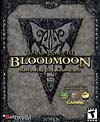
\includegraphics{media/image7.png}

{[}no fix{]} GetPCInJail (returns Boolean/short)

Bloodmoon adds a function that can be checked to see if the PC is in
Jail. The function will return 1 if traveling/in jail, zero otherwise.
This is used in the werewolf change script to stop the PC from changing
if either of these states are the case.

\textbf{Sample script:}

if ( PCWerewolf != 1 ) ; DON' RUN IF PLAYER ISN'T WEREWOLF

return

endif

if ( \textbf{GetPCinJail} == 1 )

return

endif

if ( \textbf{GetPCTraveling} == 1 )

return

endif

\hypertarget{useful-global-variables}{%
\subsection{\texorpdfstring{\hfill\break
Useful global
variables}{ Useful global variables}}\label{useful-global-variables}}

CrimeGoldDiscount (is global short)

Contains the amount of gold needed to pay the reduced fine at the
thieves guild.

CrimeGoldTurnIn (is global short)

Contains the reduced fee you have to pay when you turn yourself in.

PCHasCrimeGold (is global short)

Used in dialogue conditions. Gets set to 1 if player has enough gold to
pay for his crimes.

PCHasGoldDiscount (is global short)

Used in dialogue conditions. Gets set to 1 if player has enough gold to
pay thieves guild discount on the "price on your head".

PCHasGoldTurnIn (is global short)

Used in dialogue conditions. Gets set to 1 if player has enough gold to
the reduced crime fee that is charged when turning yourself in.

\textbf{Example:} A \textbf{dialogue result field} for the topic "price
on your head", for paying a fine at the thieves guild:

Player-\textgreater RemoveItem Gold\_001 \textbf{CrimeGoldDiscount}

\textbf{SetPCCrimeLevel} 0

\textbf{PayFineThief}

For comparison, this is the result fields that guards use when you have
a price on your head and turn yourself in (you find this under Greeting
0):

Player-\textgreater RemoveItem Gold\_001 \textbf{CrimeGoldTurnIn}

\textbf{SetPCCrimeLevel} 0

\textbf{PayFine}

Or if you get caught and have to pay the normal "fines and
compensation":

Player-\textgreater RemoveItem Gold\_001 \textbf{GetPCCrimeLevel}

\textbf{SetPCCrimeLevel} 0

\textbf{PayFine}

\hypertarget{magic}{%
\section{\texorpdfstring{\hfill\break
Magic}{ Magic}}\label{magic}}

\hypertarget{limiting-the-use-of-teleport}{%
\subsection{Limiting the use of
teleport}\label{limiting-the-use-of-teleport}}

{[}no fix{]} DisableTeleporting

{[}no fix{]} EnableTeleporting

Rather self explanatory, these functions turn the ability to use
teleporting magic on or off. Nice to keep those magic user types from
wimping out of your dungeon . In the original game it's only used when
the player encounters Dagoth Ur.

I won't show the whole script as it would be quite a spoiler, but here
is the part that uses the function:

short teleportDisabled

if ( teleportDisabled == 0 )

\textbf{DisableTeleporting}

Set teleportDisabled to 1

endif

This is later reset in the EndGame script.

\textbf{Note:} when the original Tribunal is installed this function is
effectively broken: One of the start-up scripts in Tribunal overrides
all other teleport commands and forces teleporting on except within one
specific area in Mournhold (thanks to Slink and Riiak for the info).
Here is the culprit:

\lstinputlisting{scripts/TribunalMain01.txt}

With one of the updates this problem was fixed. The latest version of
the script looks like this:

\lstinputlisting{scripts/TribunalMain02.txt}

Note: DisableTeleporting does not disable scripted amulets etc. for
teleporting. DinkumThinkum suggested the following workaround which uses
GetPCCell to check the player's current location. As long as they're in
one of the mod cells, nothing happens. If they're \emph{not} where
they're supposed to be, then the script teleports them back into the
correct area: back to the initial entry point for the mod, for example.
This wouldn't be exactly the same as blocking the teleports, but it
should make the area totally inescapable until you've fulfilled the
modder's conditions for getting out legitimately.

\lstinputlisting{scripts/DT_Test_BalmoraTrap.txt}

\hypertarget{limiting-the-use-of-levitation}{%
\subsection{Limiting the use of
levitation}\label{limiting-the-use-of-levitation}}

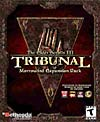
\includegraphics{media/image6.png}

{[}no fix{]} EnableLevitation

{[}no fix{]} DisableLevitation

These functions are used to allow and block Levitation magic effects.
When DisableLevitation is called, all existing Levitation effects are
canceled. When the player tries to cast a spell with a Levitate effect
while Levitation is disabled, a notify message is displayed with the
text in the GameSetting sLevitateDisabled. Currently this text reads
``Levitation magic does not work here.''

Sample scripts:

This script is on an object in the room with levitation disabled.

\lstinputlisting{scripts/clampstone.txt}

This script is on a door leaving the room.

\lstinputlisting{scripts/enable_lev_on_exit.txt}

\hypertarget{checking-and-managing-souls-and-soulgems}{%
\subsection{Checking and managing souls and
soulgems}\label{checking-and-managing-souls-and-soulgems}}

HasSoulgem, "CreatureID"

If ( Actor-\textgreater HasSoulGem, "golden saint" )

This function checks if the player has a soul gem containing the
specified soul in his inventory. A little used function that could allow
some fun quests and new uses for soulgems.

\textbf{Sample:} This is part of the StrongSoulCheck script:

if ( Player-\textgreater{}\textbf{HasSoulGem} "atronach\_storm"
\textgreater{} 1 )

Set counter to ( counter + 2 )

elseif ( Player-\textgreater{}\textbf{HasSoulGem} "atronach\_storm"
\textgreater{} 0 )

Set counter to ( counter + 1 )

endif

RemoveSoulgem, "CreatureID", number\_enum

Actor-\textgreater RemoveSoulGem, "golden saint", 1

Removes a soulgem with the specified soul from the players inventory.

Sample: this is the complementary part from RemoveStrongSoul script to
the example above:

if ( counter \textgreater{} 0 )

if ( Player-\textgreater HasSoulGem "atronach\_storm" \textgreater{} 0 )

Player-\textgreater{}\textbf{RemoveSoulGem} "atronach\_storm" 1

Set counter to ( counter - 1 )

endif

endif

Note, the player will not be happy if they get Azura's Star taken away
by this. Here's a sample solution:

short StarCount ;They could have more than one I guess.

if ( OnActivate )

if ( Player-\textgreater{}\textbf{HasSoulGem} "Golden Saint"
\textgreater{} 0 )

set StarCount to ( Player-\textgreater GetItemCount
"Misc\_Soulgem\_Azura" )

Player-\textgreater RemoveSoulGem "Golden Saint" 1

if ( ( Player-\textgreater GetItemCount "Misc\_Soulgem\_Azura" )
\textless{} StarCount )

Player-\textgreater AddItem "Misc\_Soulgem\_Azura" 1

endif

Player-\textgreater AddItem Gold\_001, 10000

MessageBox "Thank You, Come Again."

else

MessageBox "You have no Golden Saint souls."

endif

endif

AddSoulGem "creature ID", "soulgem ID"

AddSoulGem "atronach\_storm", Misc\_Soulgem\_Grand

AddSoulGem adds a soulgem of the specified type and with the specified
soul to the players inventory. You can't add more than one at a time
with this (giving it a count won't cause any problems, it's just
ignored).

DropSoulgem, "Creature ID"

DropSoulGem "atronach\_storm"

As far as I can tell, this function is broken (crashes the game).

{[}no fix{]} OnPCSoulGemUse (is short variable)

The Object is a soulgem and it has been used in either recharging or
item making

The soul gems in the game have the following ID's:

Soul Gem ID's:

Misc\_SoulGem\_Azura

Misc\_SoulGem\_Grand

Misc\_SoulGem\_Greater

Misc\_SoulGem\_Common

Misc\_SoulGem\_Lesser

Misc\_SoulGem\_Petty

This function was not used in the original game.

\hypertarget{adding-and-removing-spells-and-cursing}{%
\subsection{\texorpdfstring{\hfill\break
Adding and removing spells and cursing
}{ Adding and removing spells and cursing }}\label{adding-and-removing-spells-and-cursing}}

AddSpell, "SpellID"

RemoveSpell, "SpellID"

"Actor\_ID"-\textgreater AddSpell "Absorb Speed"

The AddSpell function will add the spell to the calling object. This can
mean two things: normal spells are added to the actor's spell list.
Curses, diseases etc, however will affect the calling object. The same
is true for the RemoveSpell function: Normal spells are removed from the
list, curses or diseases are removed as effects.

\textbf{Note:}

When you add a spell to a generic NPC, it is added to all NPCs of that
ID - unlike items, which are just added to the one NPC.

\hypertarget{some-general-notes}{%
\subparagraph{Some general notes:}\label{some-general-notes}}

You can not remove racial abilities with the RemoveSpell function (forum
info). You can remove birthsign abilities, but if the ability was added
by the player's birthsign (i.e. during character generation, not later
by script), the ability cannot be re-added afterwards (forum info /
Rocket).

(Mainly relevant for companions:) Any type of constant magical effect
(e.g. abilities, CE enchanted items, etc) on an NPC is reapplied when
the NPC changes cells, and when it gets high enough it "wraps around"
and usually starts working in reverse. Much of the time this is not
noticeable, but if necessary the problem can be avoided by removing and
re-adding the effect on CellChanged. In the case of some effects, e.g.
water breathing, the game may remove the effect too many times: in this
case SetWaterBreathing can be used (note that it must be reset after 72
game hours). (Forum info / CdCooley).

Abilities may sometimes not work as expected. If an ability is removed
by script, it may sometimes reappear after reloading a save, or later in
the game. Effects on the character's stats may also reappear or not be
removed properly on occasion (forum info / exclusiveor77). The other
problem with abilities is that damage abilities do permanent damage
(i.e. a damage health ability damages maximum health: curses do not have
this problem). This does not seem to be true of drain or fortify
effects, where it would make a lot more sense. (Forum info / ManaUser)

Curses do, however, have the problem that they can be removed by "Remove
Curse" spells.

On the Remove Curse effect, in my tests it worked but somewhat
strangely. It's percentile (like dispel rather than cure paralysis) but
the percent seemed to be cumulative or something. For example a 1\%
remove curse spell never worked (as many times as I tested it) unless I
first cast something like a 100\% remove curse spell. -(ManaUser)

\hypertarget{casting-spells}{%
\subsection{\texorpdfstring{\hfill\break
Casting spells}{ Casting spells}}\label{casting-spells}}

Cast, SpellID, "TargetID"

Object\_ID-\textgreater Cast, "flame", Player

The Cast function makes the calling object cast the spell "SpellID" on
the target "TargetID", and Target will suffer or benefit from the
effects normally. The calling object does not need to have the spell in
inventory: it will be cast regardless.

The spell's target must be specified, even if the spell is "on self". In
this case you can specify the caster or the player as the target: if the
spell is "on self" it won't make any difference. If you intend to place
the target during the game, you will still need to place a reference in
the editor. Cast will prefer a reference in the current cell if there is
one available, so there's no need to move a reference from a storage
cell: you can just place a new one.

\hypertarget{notes}{%
\subparagraph{Notes:}\label{notes}}

\begin{itemize}
\item
  \begin{quote}
  It was believed that Cast would only work on the PC. At least with
  Tribunal (not sure about earlier versions) you can use cast to cast a
  spell from an activator, or any other object, on an Actor. However,
  make sure the object you are casting the spell from is not in the
  inventory of another actor/object, as that will result in a CTD.
  \end{quote}
\item
  \begin{quote}
  You cannot force an actor to cast a spell on an activator, but you can
  have them cast on themselves, other actors, or the player.
  \end{quote}
\item
  \begin{quote}
  You can get non actor objects to cast spells on themselves. Just use
  the player (or some other object) as a target, but cast an ``On Self''
  spell.
  \end{quote}
\item
  \begin{quote}
  NPCs will not automatically lose magicka from a scripted cast. If you
  want the NPC to use up magicka in casting, this also needs to be
  scripted. -(Forum info/Kateri)
  \end{quote}
\item
  \begin{quote}
  If the spell's target is not in the current cell, the NPC will cast
  anyway (this doesn't cause any errors, but it does look a little odd -
  particularly targeted spells). They will also cast 'through' objects,
  other NPCs, walls\ldots{} anything that's in the way.
  \end{quote}
\item
  \begin{quote}
  It is entirely possible for a targeted spell to miss its target. If
  this could cause problems, it's possible to use a touch spell instead:
  it will be cast like a targeted spell (from wherever the NPC is
  standing at the time) and will always succeed, but it will have the
  same visual effects as a normal touch spell. The downside of this is
  that if you want an NPC to cast a touch spell normally (from close up)
  you need to get them into position some other way.
  \end{quote}
\end{itemize}

\textbf{Sample Script:} The cast function can be used for traps, as in
the following example attached to a Container. Note that there is a do
once condition here, so that the effect is not cast continuously on the
player.

\lstinputlisting{scripts/Trap_script.txt}

The next example script uses the \emph{AddSpell} function:

\lstinputlisting{scripts/Item_Cast.txt}

The added spell is a custom-made curse spell doing one point per second
flame damage. Note that there is again a do once condition implicit in
this script. \textbf{Failure to have a do once condition can crash the
game! Also, it appears that creatures killed with curse spell effects on
them cause all other creatures of that type to have the same curse on
them. This can be avoided by using `RemoveSpell' in an `OnDeath' section
of the script. (Forum Info / Argent)}

\hypertarget{managing-and-testing-for-spells}{%
\subsubsection{Managing and testing for
spells}\label{managing-and-testing-for-spells}}

GetSpell, "Spell\_ID" (returns Boolean/short)

If ( Player-\textgreater GetSpell, "heal companion" == 1 )

Returns true if object has Spell\_ID in inventory. However, this does
not work for abilities or powers associated with race or birthsign.
Sample script see below.

GetSpellEffects, "Spell\_ID" (returns Boolean/short)

if ( Player-\textgreater GetSpellEffects, "flame" == 1 )

Returns true if Spell\_ID is affecting calling object. The following
could be added to the "trap\_script" discussed under "casting spells"
above:

if ( Player-\textgreater{}\textbf{GetSpellEffects}, "flame" == 1 )

MessageBox "You have been flamed"

endif

This is the favorite possibility of adding new "spell effects". A dummy
spell is created that does some minimal effect, e.g. raising luck by 1
point for 1 second. The GetSpellEffects function is used to detect if
that spell has been cast on the player, and the script handles
everything else. Sample script see below.

GetSpellEffects \emph{does} work for race or birthsign abilities and
powers (with of course the proviso that the power is currently affecting
the calling object).

RemoveSpellEffects, "Spell\_ID"

Player-\textgreater RemoveSpellEffects, "flame"

Removes the effects of Spell\_ID from the player. This makes it even
more useful for scripted spells.

if ( Player-\textgreater GetSpellEffects, "flame" == 1 )

player-\textgreater{}\textbf{RemoveSpellEffects}, "flame"

;do what you want here

endif

\hypertarget{managing-and-testing-spell-effects}{%
\subsubsection{Managing and testing spell
effects}\label{managing-and-testing-spell-effects}}

GetEffect, Effect\_ID (returns short)

If ( GetEffect, sEffectRestoreHealth == 1 )

This function returns TRUE if the calling Actor is being affected by the
effect. Important: Effects are not spells, but the elements spells are
made of. In the Appendix you can find a list of all spell effects.

Don't count on GetEffect being triggered immediately when a spell is
added/cast: it will return 1 when the spell has begun to \textbf{affect}
the actor, not when the spell is cast on or added to the actor (i.e.
there's a short delay - might only be 1 frame but I didn't check).

\textbf{Note}: sEffectRestoreFatigue can't be detected using GetEffect.
-(Phaedrus). This may also be true of other fatigue-related effects
-(CaveRat).

sEffectWaterBreathing can't be detected from scripts, although it works
in the console. Luckly there is a workarround in the form of the
GetWaterBreathing function.

RemoveEffects, Effect\_ID\#\_enum

Player-\textgreater RemoveEffects, 75

Removes all spells on the Actor that include the Effect. For this
function you need the \textbf{number} of the effect-ID unlike the
GetEffect function where you need the effect ID itself (Bravo,
Bethesda!). Both can be found in the appendix.

Important: Effects are not spells, but the elements spells are made of.
In the Appendix you can find a list of all spell effects and their
number.

Sample script: This is a demonstration script that lets you check if a
spell is in inventory, if it's active on the player, if the effect it
causes is on the player and then removes the effect. Start it in the
console using "StartScript Magictest" to try it out.

\lstinputlisting{scripts/Magictest.txt}

\hypertarget{testing-disease}{%
\subsubsection{Testing disease}\label{testing-disease}}

GetBlightDisease (returns Boolean/short)

GetCommonDisease (returns Boolean/short)

If ( Actor-\textgreater GetBlightDisease == 1 )

Both functions return 1 if the calling Actor has the appropriate type of
disease, otherwise 0. These are used in the disease scripts that give
diseased or blighted creatures their disease:

Sample Script:

\lstinputlisting{scripts/diseaseBlackHeart.txt}

\hypertarget{testing-player-blight-disease-forum-info-rocket}{%
\subparagraph{Testing player blight disease (forum info /
Rocket):}\label{testing-player-blight-disease-forum-info-rocket}}

\emph{Any time the current weather is blight, the player will have
blight diseases added to them without any effects evident. They cannot
be removed with cure blight spells and getBlightDisease will continue to
return 1 for ever after unless they're removed by removeSpell. Next time
you see blight weather though, they will be back. The engine picks
random blight diseases, including any added by mods, with the exception
of those that contain the corprus spell effect. You end up with them all
very quickly.}

\emph{As a guess, I would say it's a feature (according to lore, you can
catch blight disease from exposure to blight storms) that is bugged and
was subsequently disabled, without the code being removed. So we have
this side effect. It actually breaks Bethesda's own game elements in
that the Tribunal Shrines no longer give the message that you are not
infected by blight when they should. The reason I suggest it is bugged
is that the chance to catch blight disease from blight storms is 0.10
and yet you get them very quickly. Way too quickly. It would get
annoying, even if the chance was reduced further. You catch it often
enough just from the creatures as it is.}

\emph{To disable this you need to modify the ini file. In the section
{[}Weather Blight{]} you will find Disease Chance=.10 Set this to zero.
If you then load a game where the player is currently in Red Mountain
region, it appears that you will need to wait for a weather change to
occur before the new setting takes hold (from blight to blight). Until
then, you will continue to have them added by the engine.}

Further notes:

Auto-added blight diseases that aren't showing effects make the player
effectively immune to those diseases, since the spell cannot be re-added
without first removing it (use RemoveSpell).

The dialogue function PC Blight Disease is still a reliable test, as it
only returns 1 if disease effects are present. I don't know of any
reliable way of testing player blight disease by script without
modifying the ini file, but GetSpellEffects can be used for individual
diseases (there are only four besides Corprus in the unmodded game) if
necessary.

\hypertarget{explosion}{%
\subsection{Explosion}\label{explosion}}

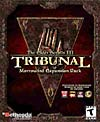
\includegraphics{media/image6.png}

ExplodeSpell ``spellName''

ExplodeSpell "proj\_trap\_spell"

The ExplodeSpell function makes a reference cast the given touch range
spell at itself. If an area effect touch range spell is used, this can
make the reference ``explode''. See the TrapProjScript, shown in the
tips and trick section on the Arrow trap.

\hypertarget{magic-getmodset-effects-functions}{%
\subsection{Magic Get/Mod/Set effects
functions:}\label{magic-getmodset-effects-functions}}

Most of these seem to refer to certain boni you normally get only from
spells. With these functions you can apparently make them permanent or
alter them. Most of these will normally use values between -100 to 100
(\%) but will accept any number, but others are flags (0 or 1). Thus,
you could make a creature that removes e.g. your ResistBlight bonus --
wouldn't that be a nice surprise for our Nerevarine?

\emph{Get/Mod/Set}ResistMagicka

\emph{Get/Mod/Set}ResistFire

\emph{Get/Mod/Set}ResistFrost

\emph{Get/Mod/Set}ResistShock

\emph{Get/Mod/Set}ResistDisease

\emph{Get/Mod/Set}ResistBlight

\emph{Get/Mod/Set}ResistCorprus

\emph{Get/Mod/Set}ResistPoison

\emph{Get/Mod/Set}ResistParalysis)

\emph{Get/Mod/Set}ResistNormalWeapons

\emph{Get/Mod/Set}WaterBreathing

Setting this to 1 enables water breathing

Get/Mod/SetChameleon

Corresponds to the Chameleon spell. This doesn't change the way the
player looks (as a spell cast would), but has the same effect otherwise,
i.e. NPCs may not detect the player and so on.

\emph{Get/Mod/Set}WaterWalking

Setting this to 1 enables water walking

\emph{Get/Mod/Set}SwimSpeed

\emph{Get/Mod/Set}SuperJump

These correspond to the Swift Swim and Jump spell effects, so they
normally range from 0 to 100, but work with negative or higher values as
well.

\emph{Get/Mod/Set}Flying

I found the following info on the UESP: This sets the player's flying
mode. To get this cheat to work, enter the console command and then cast
a Levitate Spell. The effect should now last until you disable the
flying with the console (thanks Dave Humphrey).

\emph{Get/Mod/Set}ArmorBonus

corresponds to shield effect

\emph{Get/Mod/Set}CastPenalty

corresponds to "Sound" effect? (\textless0 makes casting harder,
\textgreater0, easier)

\emph{Get/Mod/Set}Silence

\emph{Get/Mod/Set}Blindness

\emph{Get/Mod/Set}Paralysis

What it does is each paralysis effect you apply to the actor increments
the number by one. Each effect you remove decrements it by 1. You can
also alter these using the set and the mod functions. Whenever its zero
the actor can move. Try clicking on someone in the console and typing
setparalysis 1. What's good about it is if you have multiple actors of
the same ID, this allows you to paralyse an individual much like
targeting them with a spell would.\\
This is different from using a paralysis ability which would paralyse
all of that ID if you left the cell then went in again. Paralysing them
using SetParalysis lasts until you set it to zero or have gone out of
their cell for 3 days even if they are not autocalc npc's. (Forum info /
Cortex)

\emph{Get/Mod/Set}Invisibile

(Original MW: sic! Not invisible!)

\emph{Get/Mod/Set}Invisible

(Later versions of MW, apparently spelling was fixed at some point
(Forum info / Cortex))

\emph{Get/Mod/Set}AttackBonus

corresponds to fortify attack effect

\emph{Get/Mod/Set}DefendBonus

corresponds to sanctuary effect

\hypertarget{sound}{%
\section{\texorpdfstring{\hfill\break
Sound}{ Sound}}\label{sound}}

\hypertarget{make-actors-speak-an-audio-file}{%
\subsection{Make Actors speak an audio
file}\label{make-actors-speak-an-audio-file}}

Say, ``file name'', ``text''

Actor-\textgreater say,
"vo\textbackslash Misc\textbackslash CharGenBoat1.wav", "This is where
they want you."

Make subject "say" the sound file, only works on animating objects. The
.mp3 voice sound files can be found in "Data
files\textbackslash Sound\textbackslash Vo\textbackslash" folder and are
ordered in subfolders by race and gender. You can browse through most of
them in the dialogue/voice window as well. Text is what is displayed as
a subtitle as the file is played.

SayDone

Returns true if the calling object is not saying anything.

Sample Script: from character generation:

\lstinputlisting{scripts/CharGenBoatNPC.txt}

\hypertarget{playing-music}{%
\subsection{Playing music}\label{playing-music}}

{[}no fix{]} StreamMusic, ``filename.ext''

Plays the sound file "filename.ext", usually an mp3 file, as the current
music file. The music file should by default be located in the data
files/music/ folder. Stream music can also play MIDI files (JOG).

\textbf{Note:} Slightly bugged: Calling StreamMusic automatically sets
the music volume to 100, and leaves it there even after the music has
finished playing. Since there is no function to set the volume, the user
has to reset to his desired volume manually through the options menu.

\hypertarget{playing-sounds}{%
\subsection{Playing sounds}\label{playing-sounds}}

{[}no fix{]} PlaySound, ``sound ID''

{[}no fix{]} PlaySoundVP, ``sound ID'', volume\_enum, pitch\_enum

PlaySound3D, ``sound ID''

PlaySound3DVP, ``sound ID'', volume\_enum, pitch\_enum

"ex\_gg\_portcullis\_02"-\textgreater Playsound3DVP "Dwemer Door Open"
1.0 1.0

The PlaySound function plays a sound without any modification. It does
not matter to which object the script using the function is attached,
the sound will always play at full volume, directly in the player's ear,
so to speak.

The PlaySound3D function plays a directional sound source. The sound
will seem to be emitted by the object to which the script with this
function is attached.

The "VP" variants of each of these commands allow setting volume and
pitch for the sound that is played. Bethesda has not made much use of
this, it seems and it's only ever used with 1.0 set for both, which
appears to be the standard anyway. My own experiments showed the sound
not playing when I set volume to a variable, but this is no final
verdict.

The "sound ID" is the ID listed in the sound window accessed via
Gameplay -- sounds menu. You can add sounds there (place the .wav file
somewhere in Data files/sounds). A good source for sounds on the web is
\url{http://www.findsounds.com/}. Sounds should be in a certain format
(see below) so you might have to change the format in a suitable program
if you don't hear a sound in game.

\hypertarget{controlling-sound}{%
\subsubsection{Controlling sound}\label{controlling-sound}}

StopSound, "Sound ID"

Object\_ID-\textgreater StopSound "Lava Layer"

stops the sound "SoundID" if it is currently playing in the calling
object.

GetSoundPlaying, "sound ID" (returns Boolean/short)

if ( GetSoundPlaying "lava layer" == 0 )

Returns 1 when the specified sound is currently playing on the calling
object. The sound ID's can be found in the Gameplay menu /sounds and
/sound gen, where you can also set up your own (see below for formats).
This function can be used to control sounds, but also to gain
information, because certain sounds are tied to certain events in game,
e.g. the "Critical Damage" sound or the "Disarm trap" sound.

\textbf{Sample Script:} This simple script ensures that lava always has
its rumble sound playing:

\lstinputlisting{scripts/lava02.txt}

\hypertarget{sound-file-formats}{%
\subsubsection{Sound file formats}\label{sound-file-formats}}

\textbf{Note:} Not all sound files seem to play correctly in the game
(although all play in the editor). To be safe, use the formats used by
Bethesda (thanks to random name) :

"Cr" and the "Fx" folder\\
Windows PCM (.wav)\\
22050 kHz, 16-bit, Mono

Lower qualities work as well, e.g. 8,000 kHz; 8 Bit; Mono. Used e.g. in
my "The Regulars" mod for Tavern music.\\
\strut \\
"Vo" folder format\\
MPEG Layer-3, 64 Kbps\\
44100 kHz, 16-bit, Mono

\hypertarget{keeping-track-of-time}{%
\section{\texorpdfstring{\hfill\break
Keeping track of
time}{ Keeping track of time}}\label{keeping-track-of-time}}

There are a number of possibilities to follow the passage of time in
scripts, including some that are not, or only poorly documented in the
help file.

\hypertarget{timer}{%
\subsection{Timer}\label{timer}}

{[}no fix{]} GetSecondsPassed (returns float)

A simple timer can be scripted with the GetSecondsPassed function. It
returns the seconds passed \emph{since the last frame} as a float value.
To use this for a timer use something like the following example:

\lstinputlisting{scripts/TimerScript.txt}

{[}no fix{]} GetCurrentTime (returns float)

This returns the ingame time (24 hour) to two decimal places. This is
exactly the same as using the global GameHour variable, but slightly
less accurate.

\hypertarget{morrowinds-time-related-global-variables}{%
\subsection{Morrowind's time related global
variables}\label{morrowinds-time-related-global-variables}}

GameHour (is float global variable)

Day (is short global variable)

Month (is short global variable)

Year (is short global variable)

These globals get set by the game and contain the current date and time.

The MW calendar is a little bugged (thanks to samois for the info): MW
starts on Day 16, Month 7, Year 427. (16 Last seed)

The months are as follows, with the days in each month.

(Morning Star ???)

Suns Dawn 31

First Seed 28

Rain's Hand 31

Second Seed 30

Mid Year 31

Sun's Height 30

Last Seed 31

Heart Fire 31

Frost Fall 30

Suns Dusk 31

Evening Star 30

So there are 334 days in a MW year!?! Basically it seems that Bethesda
screwed up their code and lost a month, Morning Star / January\ldots{}
It seems the mistake was simply making it "wrap" to the wrong month from
Evening Star. If you manually set month to 0 it will correctly display
Morning Star in the rest menu. So this could be scripted around.

\textbf{Sample Script:} Checking the time of day with the GameHour
function:

\lstinputlisting{scripts/AfternoonTea.txt}

\hypertarget{keeping-track-of-days-passed}{%
\subsubsection{Keeping track of days
passed}\label{keeping-track-of-days-passed}}

Day (is short global variable)

Use the global ``Day'' variable. It contains the current "day of the
month" -- so on "17, last seed" it is 17. This can be used to keep track
of the number of days passed:

Short localdaysPassed

Short currentDay

if ( currentDay != Day ) ;whenever Day changes (presumably
increasing)\ldots{}

set currentDay to Day

set localdaysPassed to localdaysPassed + 1 ;add one to the counter

endif

This would usually be used for time-limited quests in a global script,
to make sure the passage of time is correctly measured. Innovative
scripting might also make use of it to trigger events after an item has
been in the player's possession for some time, etc.

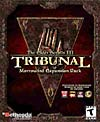
\includegraphics{media/image6.png}

DaysPassed (is short global variable)

Contains the number of days since the game started. In order to work,
DaysPassed has to be declared as a global short variable. This
declaration is present in Tribunal.esm, but not in Bloodmoon.esm. Thus,
in mods that make use of it, and that do not depend on Tribunal.esm,
DaysPassed MUST be declared explicitly. This may be one of the reasons
that some people reported it to be broken with Bloodmoon, but for others
it worked fine - it depends on whether they had Tribunal.esm checked or
not (Forum info / Erstam).

\hypertarget{moon-phases}{%
\subsubsection{Moon phases}\label{moon-phases}}

Indispensable for any potential werewolf mod.

{[}no fix{]} GetMasserPhase (returns short)

{[}no fix{]} GetSecundaPhase (returns short)

If (GetMasserPhase == 4)

{[}enable werewolf monster{]}

endif

\textbf{Note:} The helpfile lists \emph{GetSecundusPhase}, the above
syntax \emph{GetSecundaPhase} is the correct one. Also note that
GetMasserPhase and GetSecundaPhase return the value of the moon phases
for the last exterior cell you visited (Forum Info / Elim).

I only made a quick test with these, but they seem to work.

Both functions return short with these values:

0 =~MOON\_PHASE\_NEW (this is the default)

1 =~MOON\_PHASE\_WAXING\_CRESCENT or~MOON\_PHASE\_WANING\_CRESCENT:

2 =~MOON\_PHASE\_WAXING\_HALF or~MOON\_PHASE\_WANING\_HALF:

3 =~MOON\_PHASE\_WAXING\_GIBBOUS or~MOON\_PHASE\_WANING\_GIBBOUS:

4 =~MOON\_PHASE\_FULL

\hypertarget{weather}{%
\section{\texorpdfstring{\hfill\break
Weather}{ Weather}}\label{weather}}

\hypertarget{changing-weather}{%
\subsection{Changing weather}\label{changing-weather}}

{[}no fix{]} ChangeWeather, "RegionID", short\_Type\_Enum

ChangeWeather, "West Gash Region", 4

This function changes the weather in the indicated region to the weather
type specified by TypeEnum, and will change again to according to the
region settings after the time set by the game (I assume that is set in
the Morrowind.ini file in the Weather section. In mine the entry
reads:\\
Hours Between Weather Changes=20

The weather TypeEnum values are:

\begin{longtable}[]{@{}
  >{\raggedright\arraybackslash}p{(\columnwidth - 2\tabcolsep) * \real{0.35}}
  >{\raggedright\arraybackslash}p{(\columnwidth - 2\tabcolsep) * \real{0.65}}@{}}
\toprule
\endhead
0 & Clear \\
1 & Cloudy \\
2 & Foggy \\
3 & Overcast \\
4 & Rain \\
5 & Thunder \\
6 & Ash \\
7 & Blight \\
\bottomrule
\end{longtable}

\hypertarget{changing-weather-settings-for-a-region}{%
\subsection{Changing weather settings for a
region}\label{changing-weather-settings-for-a-region}}

{[}no fix{]} ModRegion, "RegionID", clear\_enum, {[}cloudy\_enum{]},
{[}foggy\_enum{]}, {[}overcast\_enum{]}, {[}rain\_enum{]},
{[}thunder\_enum{]}, {[}ash\_enum{]}, {[}blight\_enum{]},
{[}snow\_enum{]}, {[}blizzard\_enum{]}

ModRegion, "West Gash Region", 10, 20, 10, 5, 5, 40, 10, 0, 0, 0

Changes the weather chances for the RegionID. Used to get rid of, or add
weathers to an area permanently. The values must add up to 100 or you
will get odd results.

At least with Bloodmoon, all arguments except the first seem to be
optional. I am not sure if this remains true with Morrowind and
Tribunal.

If you want to maintain compatibility with a Morrowind only install, it
would be best to use only 8 arguments.

\hypertarget{determining-current-weather}{%
\subsection{Determining current
weather}\label{determining-current-weather}}

{[}no fix{]} GetCurrentWeather (returns short)

If ( GetCurrentWeather == 1 )

;{[}Do something if it is cloudy{]}

endif

This returns the weather TypeEnum listed above.

\textbf{Sample script:} Bethesda used this to make the banners move in
the wind according to weather type:

\lstinputlisting{scripts/OutsideBanner.txt}

\hypertarget{detecting-wind-speed}{%
\subsection{Detecting wind speed}\label{detecting-wind-speed}}

Undocumented:

{[}no fix{]} GetWindSpeed (returns float)

I have only very briefly tested this function and it returns values, 0
indoors and floats outdoors (varying quickly, in overcast weather the
values seemed to oscillate around 2). (Thanks to XPCagey for finding
this)

GetWindSpeed will return a value greater than 0 in interiors acting like
exteriors, which can be very useful if you need to detect an interior
acting like an exterior.

\textbf{Sample Script:} This script detects if the players current cell
is interior, exterior or interior acting like exterior.

if ( getInterior == 0 )

;outside

elseif ( getWindSpeed \textgreater{} 0.01 )

;Interior acting like exterior

else

;Interior

Endif

\hypertarget{player-sleeping}{%
\subsection{\texorpdfstring{\hfill\break
Player sleeping}{ Player sleeping}}\label{player-sleeping}}

{[}no fix{]} ShowRestMenu

Brings up rest menu, and allows the player to sleep. This is used e.g.
for beds in cells where it is otherwise illegal to sleep.

Sample Script: This is the standard script for beds:

\lstinputlisting{scripts/Bed_Standard.txt}

Returns true (1) if pc is sleeping. \textbf{Note:} The sleep selector
and counter you see while sleeping counts as a menu. So be aware of
that, if you want to use this function, and the MenuMode function in the
same script!

The \textbf{example script} seems to come from a fairly useless item,
but it demonstrates the use\ldots{}

\lstinputlisting{scripts/pillowScript.txt}

{[}no fix{]} WakeUpPC

Makes the PC wake up before the selected sleeping time is over.
Sometimes creates a monster if the player was sleeping outside. This
always happens if they try to sleep for only one hour, with longer times
it may or may not happen (Thanks to Manauser for this info). WakeUpPC
interrupts the rest only when you actually *sleep*. It does not affect
loitering in places where resting is forbidden (Forum info / Kir).

Sample script: This is an edited excerpt from the lengthy "sleepers"
script by Bethesda. It is responsible for giving you the dreams about
Dagoth Ur that plague the player during the main quest. It shows how
GetPCSleep and WakeUpPC can be used:

\textbf{if ( GetPCSleep == 0 )}

return

endif

Set dream to 0

if ( GetPCCell "Balmora" == 1 )

Set dream to 1

endif

if ( GetPCCell "Ald-ruhn" == 1 )

Set dream to 2

endif

{[}\ldots{]}

if ( dream == 0 )

Set doOnce to 0

;this makes sure you have to leave the city and come back for another
attack to occur

return

endif

AddTopic "Disturbing Dreams"

;add this topic, doesn't matter if you do it over and over

;THE FIRST DREAM...

if ( GetJournalIndex A1\_2\_AntabolisInformant \textgreater= 10 )

if ( GetJournalIndex A1\_Dreams \textless{} 1 )

\textbf{WakeUpPC}

MessageBox "You had a disturbing dream. Bla bla bla", "Ok"

Journal A1\_Dreams 1

return

endif

endif

\hypertarget{enabling-and-disabling-player-control-and-interface}{%
\subsection{Enabling and disabling player control and
interface}\label{enabling-and-disabling-player-control-and-interface}}

\hypertarget{disable-player-control-functions}{%
\subsubsection{Disable player control
functions}\label{disable-player-control-functions}}

All of these functions disable some part of the user interface, thus
restricting the players actions.

{[}no fix{]} DisablePlayerControls

Player can only look around with mouse or use options menu, nothing else
and menus disappear.

{[}no fix{]} DisablePlayerFighting

{[}no fix{]} DisablePlayerMagic

These two functions seem to be unreliable according to forum
information: If the player holds a weapon or has a spell readied he can
continue to use it and quick-keys for weapons and spell likewise still
seem to work. I currently don't know of a reliable solution for this
problem.

{[}no fix{]} DisablePlayerJumping

{[}no fix{]} DisablePlayerLooking

{[}no fix{]} DisablePlayerViewSwitch

{[}no fix{]} DisableVanityMode

\hypertarget{enable-player-control-functions}{%
\subsubsection{Enable player control
functions}\label{enable-player-control-functions}}

Once a disable function has been used, the corresponding enable function
can be used to restore control.

{[}no fix{]} EnableLevelUpMenu

{[}no fix{]} EnablePlayerControls (Enables the controls and menus.)

{[}no fix{]} EnablePlayerJumping

{[}no fix{]} EnablePlayerFighting

{[}no fix{]} EnablePlayerLooking

{[}no fix{]} EnablePlayerMagic

{[}no fix{]} EnablePlayerViewSwitch

{[}no fix{]} EnableRest

{[}no fix{]} EnableVanityMode

\hypertarget{check-player-control-status}{%
\subsubsection{Check player control
status}\label{check-player-control-status}}

All of these functions return 1 if the corresponding "Disable" function
has been called and is active, 0 if control is with the player.

{[}no fix{]} GetPlayerControlsDisabled

{[}no fix{]} GetPlayerFightingDisabled

{[}no fix{]} GetPlayerJumpingDisabled

{[}no fix{]} GetPlayerMagicDisabled

{[}no fix{]} GetPlayerLookingDisabled

GetPlayerViewSwitch

(\textbf{Broken}, function does not work. Instead use: )

{[}no fix{]} GetVanityModeDisabled

\hypertarget{force-first-or-third-person-view}{%
\subsubsection{Force first or third person
view}\label{force-first-or-third-person-view}}

{[}no fix{]} PCGet3rdPerson (returns Boolean/short)

returns 1 if in 3\textsuperscript{rd} person mode

{[}no fix{]} PCForce3rdPerson

queue the change to 3\textsuperscript{rd} person mode (this may have to
wait for the animation to finish)

{[}no fix{]} PCForce1stPerson

same as above but 1\textsuperscript{st} person mode

(See also the console command "ToggleVanityMode" (TVM).

\hypertarget{functions-for-character-generation-menus}{%
\subsubsection{Functions for character generation
menus}\label{functions-for-character-generation-menus}}

These undocumented functions are used for character creation. They
enable all the menus that are used during the character creation process
and enable certain basic features like the inventory, magic menu, stats
window and the map:

Show character generation menus:

{[}no fix{]} EnableBirthMenu\\
{[}no fix{]} EnableClassMenu\\
{[}no fix{]} EnableRaceMenu\\
{[}no fix{]} EnableNameMenu

There is no disable command for these. They are disabled by selecting ok
in the menu.

Enabling in-game menus:

{[}no fix{]} EnableMagicMenu\\
{[}no fix{]} EnableMapMenu\\
{[}no fix{]} EnableInventoryMenu\\
{[}no fix{]} EnableStatsMenu

Also no disable commands here unfortunately. These would have been
useful.

The names of the functions should be self-explanatory. One use for these
functions is as a cheat if you want to change your appearance or other
things during a running game (although there might be problems
associated with doing that). They can (and have been) used to create
different ways of character generation. Be careful, sometimes these
reset your level to 1.

\textbf{Sample Script:} This is one of many CharGen scripts that guide
the player through character generation. This one is basically a safety
feature for a player who just runs out the door, without triggering any
or all of the little tutorials.

\lstinputlisting{scripts/CharGenDoorExit.txt}

\hypertarget{determining-if-player-has-menus-open}{%
\subsection{Determining if player has menus
open}\label{determining-if-player-has-menus-open}}

{[}no fix{]} MenuMode

If ( MenuMode == 1 )

MenuMode returns one if the player has menus open, and 0 otherwise.
\textbf{This doesn't only apply to the inventory and dialogue menus.}

A good explanation is given by DinkumThinkum:

\emph{It looks to me as though the game considers 'MenuMode' to be
anytime the mouse pointer is on the screen instead of the crosshairs.
I.e., any time you can move the mouse pointer around on the screen to
select things, rather than the whole display moving and you can only
select items at the center of the screen.\\
\strut \\
For example, hitting Escape for the in-game Options menu, displaying a
message box with an "OK" button (or any other clickable buttons),
hitting '`' for the console window: all those count as menu mode, in
addition to the more obvious ones such as the dialogue window, the
character data/map/inventory screen, the container window, etc.}

It is common practice to put the following lines at the beginning of
almost any script, to prevent unnecessary or problematic functions being
processed in MenuMode:

If ( MenuMode == 1 )

Return

Endif

\hypertarget{using-menutest-to-open-and-close-menus}{%
\subsection{Using MenuTest to open and close
menus}\label{using-menutest-to-open-and-close-menus}}

Undocumented:

{[}no fix{]} MenuTest, short\_enum

MenuTest doesn't return anything, however, when it is called, it closes
certain types of inventory menus, including Player, NPC and containers.
It doesn't work for dialogue, enchanting, alchemy, spell or armorer
menus. (Forum Info / JOG, Jilin).

menutest or menutest 0 for closing menu

menutest 3 open stats menu or focus on it

menutest 4 open inventory menu or focus on it

menutest 5 open spell menu or focus on it

menutest 6 open map menu or focus on it

for menutest 3,4,5,6, it's like clicking on the upper right button of
the menu

Example Script:

if ( OnPCEquip == 1 )

set OnPCEquip to 0

coc Balmora

\textbf{MenuTest}

endif

\hypertarget{miscellaneous-functions-and-variables}{%
\section{\texorpdfstring{\hfill\break
Miscellaneous functions and
variables}{ Miscellaneous functions and variables}}\label{miscellaneous-functions-and-variables}}

\hypertarget{breaking-of-script-processing}{%
\subsection{Breaking of script
processing}\label{breaking-of-script-processing}}

{[}no fix{]} Return

Return tells the game engine to finish processing the script for this
frame. All code below this line will be ignored for this frame. In the
next frame the script is executed again \textbf{from the top}.

If ( MenuMode == 1 )

Return

Endif

Careful: Anything below a return function will not be processed, even if
there are "true" if statements there! So use this with caution.

\hypertarget{controlling-global-scripts}{%
\subsection{Controlling global
scripts}\label{controlling-global-scripts}}

These function are used to control global scripts. Global scripts have
to be started with the StartScript function (either from another local
or global script or from a dialogue result field) and a running script
can be terminated with the StopScript function.

Tribunal "Start Scripts" in a plug-in start executing each time the game
is loaded. If a Tribunal Start Script is terminated with a 'StopScript',
it will start up again the next time the game is loaded - see the Tip
and Tricks section on "Detecting when a player does a load from
savegame". (Forum info / DinkumThinkum).

To my knowledge these functions do not work with local scripts attached
to objects, you can however start and stop "targeted scripts" by using
an object "fix": "ObjectID-\textgreater StartScript" (for more info see
the Tips and Tricks section on targeted scripts).

StartScript, "ScriptName"

This starts the specified script.

\textbf{Warning:} When you use startscript, all the scripts that have
been run before you called startscript will be re-run, so scripts could
be run more than once in the same frame.

{[}no fix?{]} ScriptRunning, "ScriptName" (returns Boolean/short)

The ScriptRunning function returns 1 if a script is running, 0 if it's
not running:

if ( ScriptRunning, CharGen == 0 )

StartScript CharGen

Endif

StopScript, "ScriptName"

Stops the specified script

\textbf{Note:} If you use 'StopScript' from inside the global script
you're terminating, it doesn't actually terminate the script
immediately. Instead, the script continues executing to the 'End'
statement, and then terminates. So you still need to use "Return" if you
don't want the rest of the script to be processed.

StopScript can also be used to construct do-once conditions for global
scripts in a very clean way by self-terminating the script:

\lstinputlisting{scripts/do-once_script.txt}

\hypertarget{fading-the-screen-in-and-out}{%
\subsection{Fading the screen in and
out}\label{fading-the-screen-in-and-out}}

{[}no fix{]} FadeIn time\_float\_enum

{[}no fix{]} FadeOut time\_float\_enum

{[}no fix{]} FadeTo alpha\_enum time\_float\_enum

FadeTo 50 2.0 ;(Fades screen to 50\% in 2 seconds)

FadeIn and Fadeout fades the screen (not an object) to blackness in the
time specified (in seconds). Time is \textgreater{} 0 and \textless=
10.0. FadeTo fades only to a certain percentage: 0 is full transparency.
100 is black.

\hypertarget{adding-a-location-to-the-map}{%
\subsection{Adding a location to the
map}\label{adding-a-location-to-the-map}}

{[}no fix{]} ShowMap "cell ID"

ShowMap "Gnisis"

This function will highlight the indicated cells. Cell ID can be full or
partial, i.e. all cells that begin with the given string will be
highlighted on the world map (e.g. ShowMap "Vivec" will highlight all
the cantons).

\textbf{Sample Script:} reading this book will indicate all these places
on the world map:

\lstinputlisting{scripts/bookPilgrimsPath.txt}

Also see "FillMap" console command.

\hypertarget{assigning-random-values-to-variables}{%
\subsection{Assigning random values to
variables}\label{assigning-random-values-to-variables}}

{[}no fix{]} Random, value\_enum

Set my\_variable to Random, 50

Introducing some unpredictability into the effects of a script is a nice
option, and it can be done with the \emph{Random} function.
\emph{Random} returns values between 0 and the set value --1. So in the
example above, my\_variable will be set to a value in the range from 0
to 49.

Note that the global short variable Random100 gets set each frame by the
game's \emph{Main} script to a random value between 0 and 100
(inclusive), so you can make use of that one, too.

Note that if you are using random100 in dialogue, you may want to add:

set random100 to random, 101

in the resultbox so that random100 is reset for the next topic chosen.
Main does not set random100 in menumode.

\textbf{Note}: For any call to Random with a range over 100, the
randomosity of the return value gets very poor indeed... right up to
Random, 255 where you only get 0 or 1... and any multiple of 256 also
gets you a CTD. (Morrowind and Tribunal). In Bloodmoon, they seem to
have fixed the randomosity of the return value... you seem to get
numbers that are more evenly distributed, even with a range above 100.
But the CTD's at 256 and 512, etc, still happen (Info by Neko). It was
furthermore discovered that sometimes the Random cap is set much higher
than the number given. Setting any variable to a Random with the cap
value of one of the following numbers produces some strange result,
setting the higher cap actually to something around 1100: 65, 66, 68,
70, 71, 76, 77, 79, 82, 83, 84

TunaandCheese suggests that a method to work arround the poor
randomosity in Morrowind and Tribunal is to merge Random results, as is
demonstrated in this script:

\textbf{begin randomnumber}

\textbf{;this script works out a random number between 0 and 10000\\
\strut \\
short spare\\
short number\\
}

\textbf{;works out how many thousands there are\\
set number to random, 10\\
set number to ( number * 1000 )\\
}

\textbf{;how many hundrerds\\
set spare to random, 10\\
set spare to ( spare * 100 )\\
set number to ( number + spare )\\
}

\textbf{;and how many tens\\
set spare to random, 10\\
set spare to ( spare * 10 )\\
set number to ( number + spare )\\
}

\textbf{;this has to be random, 11, rather than random, 10 as if it was
random 10,}

\textbf{;it would only be 0 - 9999\\
set spare to random, 11\\
set number to ( number + spare )}

\textbf{;the variable number now contains a random number between 0 and
10,000 that you can use\\
\strut \\
end}

\hypertarget{playing-videos}{%
\subsection{Playing videos}\label{playing-videos}}

{[}no fix{]} PlayBink ``filename'' flag\_enum

Pauses game and plays video. Set Flag to true if player can escape
movie.

The video needs to be in Bink format and placed into the
Datafiles/Videos directory.

To convert a video to Bink format you need to use
\href{http://www.radgametools.com/bnkdown.htm}{The RAD Video Tools}.

\hypertarget{levelled-list-functions}{%
\subsection{Levelled List functions}\label{levelled-list-functions}}

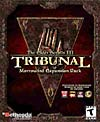
\includegraphics{media/image6.png}

{[}no fix{]} AddToLevCreature ``levcreaname'' ``creature\_ID''
level\_enum

{[}no fix{]} AddToLevItem ``levitemname'' ``item\_Id'' level\_enum

{[}no fix{]} RemoveFromLevCreature ``levcreaname'' ``creature\_ID''
level\_enum

{[}no fix{]} RemoveFromLevItem ``levitemname'' ``item\_ID'' level\_enum

These functions are used to manipulate Leveled Item and Leveled Creature
lists at run-time. Leveled lists are comprised of object/level pairs
where the level is the level the PC has to be to encounter the object.
The AddTo functions will add the given object/level pair to the
specified leveled list as long as the list does not already contain a
matching pair. The RemoveFrom functions will remove all occurrences of
the object/pair from the leveled list. \textbf{Additionally, if a
RemoveFrom function is given an object pair with a level of --1, all
object pairs containing the specified object are removed.}

\textbf{Note:} The RemoveFrom functions will not remove existing objects
from the world. If a Leveled Creature reference has already calculated
to be a certain creature, removing that creature from the Leveled
Creature's list will not get rid of the existing creature in the world.
However it will prevent that Leveled Creature reference from calculating
to be that creature again.

\textbf{Note:} The ability of creature leveled lists to call other
leveled lists is \textbf{only} in Bloodmoon. Those wishing to "nest"
creature leveled lists in their plugins must have that Bloodmoon
dependency, even if they use no objects from Bloodmoon. (forum info /
blockhead)

\textbf{Warning:} It is not recommended that you use these functions as
it will break any other mod that uses leveled lists.

DarkDragon writes on the Official forums:\\
\emph{The problem lies in the way Morrowind loads items. First it loads
ESMs, then ESPs, which can modify the leveled lists. If you have a list
merger, you can merge those lists and keep the changes from all of them
(where as before, the last loaded mod would take precedence). Then it
loads ESS, or save files.}

\emph{\hfill\break
The problem is, if a script adds something to a Leveled List, it
modifies the ESS (save game) and the save game then has a reference to
that Leveled list. This is loaded last and it overwrites ANY changes
done by other mods.}

Sample Script:

When this script is placed on an object, activating it will toggle the
existence of rats in the world by removing them from a Leveled Creature
and removing rat meat from a Leveled Item.

\lstinputlisting{scripts/norats.txt}

\hypertarget{square-root}{%
\subsection{Square root}\label{square-root}}

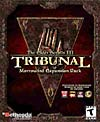
\includegraphics{media/image6.png}

{[}no fix{]} GetSquareRoot, number (float)

set var\_1 to GetSquareRoot var\_2

The GetSquareRoot function returns the square root of the given number.
This can be useful for vector or distance calculations (remember
Pythagoras?).

It is possible to get the square root of a number without using this
function, however it is significantly slower. See Soralis's Math mod for
an example script. MWSE also has a square root function.

\hypertarget{water-level-functions}{%
\subsection{Water Level Functions}\label{water-level-functions}}

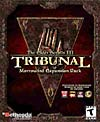
\includegraphics{media/image6.png}

{[}no fix{]} GetWaterLevel (float)

{[}no fix{]} SetWaterLevel newWaterLevel\_float

{[}no fix{]} ModWaterLevel waterLevelChange\_float

A great opportunity for cruel traps\ldots{} These functions are used to
determine and modify the Water Level of the current interior cell. When
an Actor suddenly finds itself underwater, it will wait until it is
halfway out of breath and then begin to make its way to the surface in a
straight line up. Floating corpses are moved with the water without
regard for collision.

\textbf{Note:} If you use GetWaterLevel in a interior cell with no
water, GetWaterLevel will still return a result other than 0.

\textbf{Note:} Set/ModWaterLevel doesn't work in exteriors.

Sample scripts:

This script goes on a crank to make it raise or lower the water level in
the room.

\lstinputlisting{scripts/crank.txt}

This modified ``Float'' script is placed on any object with a centered
pivot point to make it float on the water's surface regardless of water
level. It also will make the object stop bobbing if the PC is standing
on it.

\lstinputlisting{scripts/NewFloat.txt}


% Chapter sectioning
\hypertarget{tips-and-tricks}{%
\section{\texorpdfstring{\hfill\break
Tips and tricks}{ Tips and tricks}}\label{tips-and-tricks}}

\hypertarget{little-helpers-text-search-copy-paste}{%
\subsection{Little helpers: Text search, copy,
paste}\label{little-helpers-text-search-copy-paste}}

A good function to use for the beginning scripter is the search text
function in the main TESCS edit menu. You can use it to search scripts,
e.g. for a specific function you would like to use and want to find
sample scripts for.

You can also use any text-editor, or the alternative scripting editors
listed below for editing your scripts and copy / paste the script to and
from the TES CS editor using ctrl-c / ctrl-v.

To make a copy of a script you want to change, don't just change the
name, this will just overwrite the old script. Instead copy the original
script (ctrl-a, ctrl-c) start a new script and paste the old one in
(ctrl-v) now rename the script and change what you need.

\hypertarget{alternative-scripting-editors}{%
\subsection{Alternative scripting
editors}\label{alternative-scripting-editors}}

1) MentalElf created an Elder Scrolls Scripting mode for the venerable
\textbf{EMACS} coding editor, including automatic tabulation of
if-blocks, and color coding of script code.:

\url{http://www.mentalelfz.com/}

EMACS is available for free under the gnu license (link is on MetalElf's
page).

2) UESP's Dave Humphrey created \textbf{MWEdit,} an alternative
construction set with improved scripting support (This is a beta
version. I have only tested it briefly, but it looks very good, and
seemed quite stable): \url{http://mwedit.sourceforge.net/}

Regarding scripting, Dave lists the following features:

- Color coding of script code. Use a default white or blue color scheme
or use any custom colors to identify the various word types. Can also be
disabled. (\emph{see the trigonometry script below for an example of the
color coding})

- Select the font used in the script window.

- New script compiler reports many more errors and possible errors.

- Three levels of warning/error messages (weak, default, and strong)
allowing you to set how many compiler messages are recorded.

- Compiler adds spaces to the script output where they might be required
or expected (such as in if statements).

- Object types used in functions are checked more rigorously. If the
function expects an NPC ID, you'll receive an error/warning if you use
another type.

- Compiles script on save automatically (no warning/errors displayed).

- Export and import scripts to/from text files.

- View detailed help on all script functions.

- All compiler errors/warnings are displayed in a splitter pane at the
bottom of the script window. Double-click a message to jump to the
location of the message.

- View detailed information on compiler messages and display the
function help if the message is related to a specific function.

- Compiler does not permit the use of reserved words as local variables
(such as end, X, Y, etc...).

- Functions that are known to be broken will result in a compiler
message.

- Simple function tooltips can be displayed for faster scripting.

\hypertarget{script-extenders}{%
\subsection{Script Extenders}\label{script-extenders}}

Script extenders are programs that need to be run at the same time as
Morrowind to work, they add new functions to the Morrowind scripting
language.\\
This is by no means a guide to 3\textsuperscript{rd} party programs; it
is intended to give a brief overview. To find out more, it is
recommended that you download the programs/dev kits.

A list of mods made using script extenders that should give an overview
of what is possible:\\
http://www.mwmythicmods.com/MWE.htm

Morrowind Enhanced (MWE):

\url{http://planetelderscrolls.gamespy.com/View.php?view=Utilities.Detail\&id=8}\strut \\
Adds many new functions, including getting references and using them
with the vanilla Morrowind functions. It also adds better sound
detection, skill leveling functions and functions to manipulate spells.

Scripts are written in the TESCS, with functions using unused commands
like ToggleLoadFade. The esp then has to be processed by another
compiler.\\
Unfortunately it is no longer being developed.

Morrowind Script Extender (MWSE):\\
\url{http://sourceforge.net/projects/mwse/}

MWSE is fairly similar to MWE in some respects, as it can get
references, and then use those references with other default functions.
It adds more functions than MWE, and is still being developed. It is
slightly harder to code with, in that the MWSE functions cannot be used
within normal if blocks, only within new ifx blocks, which have some
drawbacks. However, the script readability is improved as it uses words
for functions rather than cryptic unused commands and variable settings.

To compile MWSE scripts, you need to use MWEdit\textbf{.}

Morrowind Graphics Extender (MGE):

\url{http://www.tesnexus.com/downloads/file.php?id=5535}\strut \\
MGE mainly allows manipulation of the rendering to the screen, so if you
want to draw a texture to the screen, it is the program you want. It
also allows you to apply shaders to the screen, press keys, manipulate
the mouse, use bumpmaps and other graphics related features.

It requires MWSE (Included in MGE), and scripts are compiled using
MWEdit

\hypertarget{script-with-style-for-safer-scripting}{%
\subsection{Script with style for safer
scripting}\label{script-with-style-for-safer-scripting}}

This is bound to be a bit controversial as it is as much about personal
style as it is about fact. And it's bound to sound snobbish .
Nevertheless, I think this might be of some use for the newcomer, so
here are a few comments about my personal views on good style and safer
scripting:

\begin{itemize}
\item
  Use annotations. In a really short script they might seem useless, but
  even there you might want to state which mod/quest/item they belong to
  or what their general purpose is, etc. For long scripts this becomes
  indispensable, for yourself, if you stop working for a few days as
  well as for others that might want to learn from your script. Explain
  your variables, put headers on the main part of your script, comment
  on important lines of code, etc.
\item
  Use state variables with style. Basically, due to the "executed once a
  frame" nature of the scripts this is your principal way of structuring
  your script for sequential events. There are several things to this.\\
  A) Limit yourself to the minimal amount you need for the script.\\
  B) use elseifs to chain different states of one state variable
  together, not separate if-blocks -- this should be the main structural
  element of your script (it's not always possible nor necessary, but if
  it is, its going to save you a lot of trouble).\\
  C) Check the elseifs are arranged from lowest to highest and in a
  logical order of events -- will help you to keep everything organized,
  and thus avoids bugs. Jumping around wildly with state variables is
  the equivalent to careless use of GOTO in good old BASIC.\\
  D) Use them extensively, do small steps. I can't tell you how many
  times bugged scripts started working simply because I moved some
  functions to a separate "state-block". Sometimes this doesn't seem to
  be logical at all -- but if you can safely enter another step, do it.
\item
  Decide for one style. TES Script is relatively forgiving regarding
  syntax. You can write functions small letters or capitalized as in
  this document, or all caps. You can use if ( SomeFunction == 1 ) of if
  (somefunction). But whatever you choose, try to be consistent in your
  usage.
\item
  Use verbose variable names. A name that reflects the function of this
  variable makes a script much more readable. If you use global
  variables give them a unique name, e.g. put your initials in front or
  whatever -- just try to minimize the chance that another mod will come
  up with the same name for a global -- because that would screw things
  up royally.
\item
  Keep track of your Return function uses. The Return function is
  inherently dangerous -- remember that it will stop anything in that
  script below that line from being executed. Use it, but use it
  sparingly. If you have the feeling you have to use it a lot in one
  script, you should probably introduce a state variable instead.
\end{itemize}

\hypertarget{cleaning-up-your-mod}{%
\subsection{\texorpdfstring{\hfill\break
Cleaning up your
mod}{ Cleaning up your mod}}\label{cleaning-up-your-mod}}

When you work on your mod, you will probably want to look up other
things as reference or simply to cut and copy things for your own
purposes. The problem is that the TESCS will remember you looked at the
things if you moved them the slightest bit in the game world, or if you
ever hit an ``OK'' button, even if you did not change anything. Before
you release your mod you should check it for such unwanted references
and remove them.

In the File Menu select Data Files. Then select your mod like you
normally would and hit the Details button. Look at the list of features
here: this is a list of everything your mod changed or added. Look for
things that you did not want to change, and select them.

Select a single item with Left Click.

You can select multiple items using Ctrl + Left Mouse Button.

If you click on an item and then use Shift + Left Click on another item,
everything in between will be selected.

You don't have to select everything you want to remove at once, you can
do it in multiple deletes.

To remove items, hit {[}del{]} on your keyboard. This marks the feature
as ignored. Loading and resaving the mod will remove these ignored
features from the mod.

An alternative, and much easier to use is the utility TESAME (TES
advanced mod editor), available from various sites, e.g.:

\url{http://theseventhrealm.com/portal/tools.html}

A more recent tool that has become indispensable to me is the Morrowind
Enchanted Editor, available at:

\url{http://tfo.rh.rit.edu/esforum/secretmasters/EnchantedSetup0.91c.exe}.

It's not very well documented, but offers a much nicer user interface
than TESAME and is immensely powerful.

For scripts, try to remove any unused global variables or whole scripts
you may have made in the course of developing your script. It bloats
your .esp filesize, it probably wastes memory, or at the very least it
looks bad.

This is a list of the change indicators found in the details tab of
TESAME:

DIAL -- A new or changed topic

INFO -- A dialogue response, or journal entry

REFR -- a reference of an object that was put into the game world, while
MISC, CONT etc. describe the actual Object (even if there is no instance
of it placed in the world)

SOUN -- A Sound

NPC\_ - A new type of NPC, or a changed NPC

CREA -- A new creature or a change to a creature

LIGH -- A new or changed Light

LTEX -- An application of a landscape texture

PGRD -- A change to the AI grid

CELL -- obvious, signifies a changed cell either indoors or outdoors --
in case your mod had nothing to do with that cell you should get rid of
it. This affects all changes in that cell automatically, I think
automatically

SCRPT -- A Script -- lots of people leave superfluous "test scripts" in
their mods -- that's bad style, I think.

MISC -- A new or changed miscellaneous object -- check names, delete if
the change is unrelated to your plugin

ACTI -- An activator -- see above

CONT -- A container -- very critical: make sure you only change a new ID
(copy of a container), not the original container -- or they will all be
changed.

STAT -- A static object -- see above

\hypertarget{on-references-persist}{%
\subsection{\texorpdfstring{\hfill\break
On References
Persist}{ On References Persist}}\label{on-references-persist}}

The object windows in the TESCS have a checkbox named "References
persist". Ticking this checkbox ensures that a reference (an instance of
the object in the game world) is always available to be referenced by
script, even if the player is in a different cell, or has not yet
encountered the object.

If a script uses a specific reference to an object such as

RefObject-\textgreater Enable

Then "RefObject" should have References persist checked.

Indirect referencing such as;\\
PlaceAtMe my\_object 1 1 1\\
Player-\textgreater AddItem my\_object 1

do not usually require references persist. Some functions may be
exceptional in this respect. For example;

GetDistance, RefObject

requires that RefObject has been placed in the world and references
persist checked.

Actors (NPC and Creatures) are always persistent.

(Thanks to Nigedo for additional information)

\hypertarget{the-72-hours-bug-a-brief-explanation}{%
\subsection{The "72-Hours Bug": A Brief
Explanation}\label{the-72-hours-bug-a-brief-explanation}}

(Thanks to DinkumThinkum, Emma, Iudas, Qarl and others for this
information.)

The so-called "72-Hours Bug" is not really a bug at all - nor is it
necessarily 72 game hours. The time is set by fCorpseClearDelay (see
"Game Settings"), which defaults to 72, and which also controls the
delay before non-persistent corpses vanish. After the specified time,
some temporary data is cleared to improve game performance.

Examples include:

\begin{itemize}
\item
  Talked to PC flag (dialogue) is reset.
\item
  ForceGreeting: an actor will not be available for a ForceGreeting
  after the specified time unless "Corpses persist" is checked in the
  object info box.
\item
  Actor stats and skills are reset to editor/autocalc levels.
\item
  AI resets: e.g. an actor in combat with the player but with a low
  fight setting will no longer attack.
\item
  Targeted scripts on non-persistent objects lose their targeting.
\item
  OnActivate may be reset (see function description for more details).
\end{itemize}

Specific workarounds are mentioned in the relevant function's
description. Alternatively, other methods can be used to store
information. For example:

\begin{itemize}
\item
  A script that runs at least once each load session can be used to keep
  track of information, e.g. a companion's stats and skills.
\item
  Journal entries or global variables can be used to store information,
  e.g. as a substitute for the Talked to PC flag.
\item
  Token items may be added to an actor's inventory (or a refs persist
  container).
\end{itemize}

Of course, other workarounds may be devised. Note that it is usually not
advisable to change the value of fCorpseClearDelay, as GMSTs are not
accessible to script and your change may break mods which rely on
time-dependent methods of avoiding the loss of temporary data. (Changing
the setting to a \emph{higher} value is less likely to break other mods,
but more likely to cause CTDs for those whose system can't cope with the
amount of data stored.)

\hypertarget{limits-of-the-script-editor}{%
\subsection{Limits of the Script
Editor}\label{limits-of-the-script-editor}}

\textbf{Character Limit:} There is a limit of the maximum number of
characters per script. It is somewhere around 30000 characters ( the
true limit is most likely 32767, which is the max value for a 16-bit
signed integer, which is how script length is stored in the .esp --
thanks to Horatio for this info). If this occurs you can no longer type
in the editor window. To save characters try the following:

\begin{itemize}
\item
  Remove characters
\end{itemize}

\begin{itemize}
\item
  Use shorter variable names
\item
  See if the script can be split and some part maybe handled in a global
  script or attached to a separate object as a separate script.
\end{itemize}

\textbf{Line Limit:} there also is reportedly a maximum line limit. This
seems to vary and reports on the forum range between 900-and 1500 lines
of code. It's probably rather a limit of the compiled script than the
actual lines of text, so empty lines and comments don't count. This is
reported by an error message upon saving the script.

\textbf{If-elseif limit:} There is a limit on the maximum number of
if-elseif conditions that can be used per script. I am not sure of the
absolute number (I heard both 127 and 256). Also there is a maximum
depth of nested if commands, it's reportedly 10 (thanks Riiak).
\emph{(Note: Error message for exceeding the maximum depth of nested
if's is "Max nesting of 10 exceeded on line XXX" - in this case, you'll
need to break it up somehow.)}

\textbf{Instruction Limit:} An If-block or While-block is limited to 255
compiled commands (per block, not per script). The limit is \emph{not}
on the number of lines (each line may end up as several commands when
compiled), and blank lines and comments don't count towards this total.
-(Dave Humphrey, thanks to Galsiah for pointing this out)

\hypertarget{script-name-limit-tunaandcheese-reported-a-limit-to-the-length-of-the-scriptname-your-scripts-name-should-never-go-over-31-characters-in-length.-it-if-you-have-32-characters-in-the-script-name-there-will-be-a-box-on-the-end-of-the-script-and-when-there-is-33-characters-the-33rd-character-goes-funny-the-34th-character-seemed-to-be-fine.}{%
\paragraph{\texorpdfstring{\textbf{Script Name Limit:} TunaandCheese
reported a limit to the length of the scriptname:\\
Your script's name should never go over 31 characters in length. It if
you have 32 characters in the script name there will be a box on the end
of the script and when there is 33 characters the 33rd character goes
funny, the 34th character seemed to be
fine.}{Script Name Limit: TunaandCheese reported a limit to the length of the scriptname: Your script's name should never go over 31 characters in length. It if you have 32 characters in the script name there will be a box on the end of the script and when there is 33 characters the 33rd character goes funny, the 34th character seemed to be fine.}}\label{script-name-limit-tunaandcheese-reported-a-limit-to-the-length-of-the-scriptname-your-scripts-name-should-never-go-over-31-characters-in-length.-it-if-you-have-32-characters-in-the-script-name-there-will-be-a-box-on-the-end-of-the-script-and-when-there-is-33-characters-the-33rd-character-goes-funny-the-34th-character-seemed-to-be-fine.}}

Character 32 gets replaced by some other character in the title bar and
in the Details list information. From looking at the .esm/.esp/.ess
format information on Argent's web site, apparently only 32 bytes are
allocated for the script name, which makes a 31 character limit
reasonable. -(DinkumThinkum)

\hypertarget{pitfalls}{%
\subsection{Pitfalls}\label{pitfalls}}

\hypertarget{inconsistent-commas}{%
\subparagraph{Inconsistent Commas}\label{inconsistent-commas}}

The scripting language is fairly forgiving in terms of comma usage or
not, but the inconsistent use of commas can cause difficulties:

This will work:

Player-\textgreater PositionCell, -1396, 124, 3312, 90, "Cell ID"

and this will work:

Player-\textgreater PositionCell -1396 124 3312 90 "Cell ID"

but this will sometimes have problems:

Player-\textgreater PositionCell -1396, 124, 3312, 90 "Cell ID"

\hypertarget{object-names}{%
\subparagraph{Object Names}\label{object-names}}

Don't start object names with an underscore. Otherwise, some script
operations will fail.

This will cause runtime error.

\_wr\_testNPC-\textgreater forceGreeting

This will work fine

wr\_testNPC-\textgreater forceGreeting~;-\/-Okay.

\hypertarget{fractional-numbers}{%
\subparagraph{Fractional Numbers}\label{fractional-numbers}}

A constant float specified without digit before the decimal point will
cause a runtime error. Floats in the range: -1 \textless{} 0 \textless{}
1 should be specified with a leading '0'. Otherwise you'll experience a
runtime error.

This gives you a runtime error

if ( number == .2 )~

This runs fine

if ( number == 0.2 )

34th Variable

If you have a script with 34 or more variables of the same type (short,
long or float), the 34th variable of that type can cause errors when
used. For that reason, most scripters call it "DoNotUse" or something
like that to remember that they should not use it. The reason for this
problem seems to be that the ASCII character 34 is the double quote
character.

Short 32ndVar

Short 33ndVar

Short DoNotUse ;Really the 34\textsuperscript{th} Var

Short 34thVar

Short 35thVar

\hypertarget{saving-cpu-time}{%
\subsection{\texorpdfstring{\hfill\break
Saving CPU time}{ Saving CPU time}}\label{saving-cpu-time}}

If you plan a mod with lots of scripts or long and involved scripts, you
may want to give some thought to not wasting CPU power. There are a
number of things you can do here:

If the script does not have to be executed every frame, \textbf{put a
little counter in there}:

\lstinputlisting{scripts/My_super_long_script.txt}

This little piece of code, that should be at the very top of your
script, will allow your script (or rather the main, CPU power eating
part of it) to be executed only every 10\textsuperscript{th} frame. You
could do the same thing with a timer, and execute the script only every
3 seconds or once every minute.

\textbf{Execute script only if the player is suitably near.} If you have
scripted a fancy magic bouncing ball, or basically anything that is a
visible effect, there is no reason to run the script if the player
cannot see it. So put something like this on top of your script:

If ( GetDistance, player \textless{} 5000 )

Return

Endif

However, as getDistance isn't an amazingly fast function, you wouldn't
want to put this check above a simple getScale, setScale script.

\textbf{Shortcut scripts that are no longer needed.} If you have local
scripts that you may not need from a certain point onwards, e.g. because
of Actor death or because the object was disabled, reduce their CPU need
by putting something like the following at the top of the script:

if ( GetDisabled == 1 )

Return

Endif

If ( GetHealth \textless= 0 )

Return

Endif

\textbf{Terminate global scripts.} Remember, global scripts are running
all the time until you stop them again with StopScript. You can do
do-once global scripts by just putting a StopScript command at their end

\lstinputlisting{scripts/do_once_global_script.txt}

\textbf{Try to use local scripts} instead of global scripts. With local
scripts you are sure that they only run when you are in the vicinity.
Think hard before making a script global if it can be done with a local
script instead.

\textbf{Be careful with while-loops, GetDetected, GetLOS} and other
"slow" functions. Use methods as described above (e.g. a counter or a
timer) to make sure they are not called too often.

\textbf{Stop script while in menu mode.} Always, unless you have
specific reason not to, put the following at the top, to avoid the mouse
lagging in the menu and other unwanted effects.

If ( MenuMode == 1 )

Return

Endif

\hypertarget{section-12}{%
\subsection{}\label{section-12}}

\textbf{In general, reducing the number of scripts running improves
efficiency} more than reducing the complexity of individual scripts.

So, for example, if you have two short globals running all the time, it
is better to merge them into one global.

If you've got a few global scripts which only need to run based on some
check, it makes sense to place the checks in one "parent" script, and
startscript the others from there when they need to run (remembering to
ensure to run them once per game session if they need to conserve
variable values).

\hypertarget{targeted-scripts-running-global-scripts-tied-to-an-object}{%
\subsection{\texorpdfstring{\hfill\break
Targeted scripts: running "global" scripts tied to an
object}{ Targeted scripts: running "global" scripts tied to an object}}\label{targeted-scripts-running-global-scripts-tied-to-an-object}}

"Object\_ID"-\textgreater StartScript "Script\_ ID"

\emph{(Credit for discovery of this technique and much of the following
information goes to FreshFish. Further information supplied by Riiak,
MentalElf, DinkumThinkum, Argent, Cortex, and others.)}

It is possible to use the StartScript function to run global scripts
that are tied to an object or Actor. These scripts resemble both local
scripts (in that the functions called always default to the object or
Actor the script targets) and global scripts (in that they are always
running). Objects may have several different targeted scripts running on
them at one time, and may also have a local script.

\hypertarget{to-start-a-script-as-a-targeted-script}{%
\subparagraph{To start a script as a targeted
script:}\label{to-start-a-script-as-a-targeted-script}}

\begin{itemize}
\item
  Object\_ID-\textgreater StartScript Script\_ID (may be used from
  script, but does not work from dialogue results).
\item
  Start the script from the intended target's local script or another
  targeted script on the object (it will inherit the target).
\item
  Start the script from dialogue results (this will only work to target
  the actor the player is in dialogue with: it is not possible to
  specify a different target in dialogue results). This method is
  particularly useful as you don't need access to scripts running on the
  actor, nor do you need an ID.
\end{itemize}

\hypertarget{uses-of-targeted-scripts}{%
\subparagraph{Uses of targeted
scripts:}\label{uses-of-targeted-scripts}}

As a general rule: If a function requires a fix in a global script but
the fix can be omitted in a local script, that function may be used
without a fix in a targeted script as well. Examples of popular
functions for targeted scripts include:

AddItem, RemoveItem, GetItemCount

AIFollow, AIWander, AIEscort

GetPos, SetPos, PositionCell

Get/Set/Mod\emph{Stat}

StartCombat, StopCombat

Targeted scripts can be powerful tools, especially in combination with
dialogue: you can create generic dialogue (e.g. filtered for class only)
and start your script from the resultbox. CDCooley's "Companion
Teleportation" is a good example of use with dialogue. Voice dialogue
can also be used this way: for example, many companions have a targeted
"pacifist" script that is started from Attack voice results if the
player tells the companion to avoid combat.

\hypertarget{cautions-and-limitations}{%
\subparagraph{Cautions and
limitations:}\label{cautions-and-limitations}}

\begin{itemize}
\item
  Variables defined in a targeted script are not considered local to the
  object from the point of view of dialogue and other scripts. For
  example, they cannot be used as dialogue conditions. The special
  variable "companion" also cannot be used, i.e. declaring a short
  variable "companion" in a targeted script and setting it to 1 will not
  enable companion share on the target actor. I assume this applies to
  other special locals as well, but I haven't tested any others.
\item
  You cannot have more than one instance of a targeted script running at
  one time (same as global scripts). The obvious workaround is to have
  several different scripts that all do the same thing.
\item
  If OnActivate is used in a targeted script, the object will not be
  able to be activated by normal means after the script is stopped,
  unless a targeted script with an OnActivate is again added to the
  object.
\item
  If an object is deleted while a targeted script is running on it, the
  game will CTD. If the target is not necessary but is merely a
  consequence of the way the script was started, you can usually target
  the script on the player instead to avoid this:
  "player-\textgreater StartScript ScriptName". Otherwise, the script
  must be stopped before deleting the object.
\item
  Scripts will detach from non-persistent targets when the game is saved
  and reloaded. This may give errors on load ("Unable to locate
  reference for global script\ldots"), or may not; either way it may
  also give odd effects in some circumstances.
\item
  When a targeted script is started on an object that was not placed
  into the gameworld in the editor (i.e. an object that was placed or
  generated during the game), the script will lose its targeting when a
  savegame is reloaded. Note that this applies to the player character
  as well.
\item
  Load list changes may also cause targeted scripts to lose their
  targeting when the game is reloaded, whether or not the target is
  persistent and whether or not it was placed in the editor. This
  doesn't always happen, but it can (adding several mods higher in the
  load list will usually do it).
\end{itemize}

If a script becomes detached from its target, some functions that
manipulate data about the previously targeted object (e.g.
getHealthGetRatio) may cause CTD if used without a fix.

As a workaround to avoid untargeted scripts running, you may be able to
use a startscript to stop the targeted script if it is running, then
restart it if necessary. As a safety check for targeted scripts on
actors, GetHealth may be used before any functions that may cause
problems (returns 0 in an untargeted script):

if ( GetHealth \textless= 0 )

StopScript ScriptName

return

endif

; main body of script goes here

\hypertarget{detecting-when-the-player-does-a-load-from-saved-game}{%
\subsection{Detecting when the player does a load from saved
game:}\label{detecting-when-the-player-does-a-load-from-saved-game}}

Some reasons to test for player loading a saved game:

1) To continue custom music (mp3 type music resets on load).

2) To keep a NPC running or sneaking.

3) To reset an object to its proper scale (if outside of range 0.5 to
2.0).

There are a number of ways to do this:

JOG proposed the use of SetJournalIndex:

if ( ( getjournalindex "dummy" ) != 100 )

Messagebox "You just reloaded, Cheater!!!"

setjournalindex "dummy" 100

endif

"Dummy" is any journal-topic that has no text for index 100.

Setjournalindex will set the index to the new value, no matter if an
entry exists for this value or not, but when you reload, the index will
be reset (see SetJournalIndex for more information).

MentalElf suggested that GetForceRun, GetForceSneak, GetScale can all be
used to detect when the player has just loaded a save game. This is due
to ForceRun and ForceSneak being cleared during a load from saved game,
and scale is set to within the range 0.5 to 2.0. In my opinion ForceRun
is best, as ForceSneak puts the NPC into a crouch posture.

; (NPC object)

if ( GetForceRun == 0 )

; Player just loaded a saved game

; Handle game load here.

ForceRun

Endif

A different option is to use start scripts ( available only with
Tribunal and Bloodmoon): Here are two examples by Dinkum Thinkum:

\lstinputlisting{scripts/DT_DoOnce_TribStartScript02.txt}

\lstinputlisting{scripts/DT_DoOnce_TribStartScript01.txt}

\hypertarget{uses-of-the-chargenstate-variable---disabling-saving-and-menus}{%
\subsection{Uses of the CharGenState variable - Disabling saving and
menus}\label{uses-of-the-chargenstate-variable---disabling-saving-and-menus}}

The availability of the save option in the main menu (and the Quicksave
key) depends on the value of the CharGenState global. Set it to
something other than -1 (to 99, for example), and the player is no
longer allowed to save the game. Setting CharGenState back to -1 again
turns everything back to normal.

This has several side effects. First, you won't be able to access the
menu screen. This can be fixed by EnableStatsMenu - it reenables ALL the
menus, not only the stats window. However, the journal, the Quick Keys
and the QuickKey menu (F1) are disabled as well, and you can't loot
corpses. I haven't found a way around these limitations.

There is some conflict potential in this, so it would be good to take
some precautions that the player is not currently inside the character
generation sequence, and that the value is set back to its original
value after use.

(Forum info / Erstam)

\textbf{Note:\\
}If you use a command like EnableStatsMenu or EnableInventoryMenu while
CharGenState is other than -1, you will never be able to turn off the
menus again with CharGenState. The EnableInventoryMenu command only
seems to have this effect in the CharGen process, while EnableStatsMenu
has this effect all the time. If the menus were supposed to be turned
off in a mod, it won't work. You still can't save or use quick keys. But
what really is annoying about this is that this applies for the whole
game session! You actually need to exit the game and restart it, so you
can never rely on that menus will be turned off.

(Forum info / Björn )

\hypertarget{detecting-use-of-scrolls-or-books}{%
\subsection{\texorpdfstring{\hfill\break
Detecting use of scrolls or
books}{ Detecting use of scrolls or books}}\label{detecting-use-of-scrolls-or-books}}

This is a surprisingly difficult task, as OnActivate and OnPCEquip are
both needed AND don't work quite as expected. Kir has found a solution
as shown in this script for invoking a letter of credit:

\lstinputlisting{scripts/BankLetter10.txt}

Erstam posted a script with even better features, that also revealed an
interesting glitch with the scripting variables OnPCEquip / SkipEquip:

"Inspired by the BankLetter script in MSFD 7, I have found a way to run
custom script code on books and scrolls when either "equipped" from the
player's inventory or activated from the game world, \emph{while the
book/scroll is displayed as normally}. Surprisingly, it's the
PCSkipEquip variable that is set to 1 when the book is dropped on the
player's portrait, rather than the OnPCEquip variable. This is the code
I used:"

\lstinputlisting{scripts/activateBook.txt}

It should work without the doOnce condition, in case you want the action
to take place every time you equip the book, but I haven't tested it
yet.

\hypertarget{making-actors-switch-between-weapons}{%
\subsection{\texorpdfstring{\hfill\break
Making Actors switch between
weapons}{ Making Actors switch between weapons}}\label{making-actors-switch-between-weapons}}

Since the equip function does not work, the only way to do this is to
take items away from the Actor, or to modify his skills at runtime.

Here is an example I used to make a guard switch between bow and sword:

\lstinputlisting{scripts/HBCaravanGuardAI.txt}

The next example is one by Bethesda, which does the same thing, using
the skill change method (admittedly more elegant than mine ):

\lstinputlisting{scripts/marksmanToggle.txt}

\hypertarget{making-npcs-switch-between-spell-sets}{%
\subsection{Making NPCs switch between spell
"sets"}\label{making-npcs-switch-between-spell-sets}}

If you want an NPC to switch between different sets of spells, the
skill-setting method will not work unless the spells are grouped into
different schools (which is unlikely to be the case). Adding and
removing spells will only take effect when the NPC is not in combat, but
StopCombat will stop combat for all actors involved (usually not a good
idea). However, other AI commands can be used to stop combat for a
single character. This method is more useful for followers of the player
than for hostile NPCs as the character will exit combat, however
briefly: since the enemy will generally attack the player rather than a
follower, temporarily removing a follower from combat is unlikely to
cause problems; using AIFollow to remove the follower from combat
ensures that the NPC will immediately re-enter combat at the first hit
by or on the player. AIWander (and probably other AI commands) will also
work, but you may need to restart combat using StartCombat afterwards.

The following example is an abbreviated snippet from the local script of
a companion I'm working on. Most of the time the spell-switching is
barely noticeable (just a moment of hesitation), and the companion
quickly re-enters combat.

;CombatStyle is set from dialogue when the player gives combat orders

if ( CombatStyle == 1 ) ;switch between targeted and touch spells

if ( player-\textgreater GetSpellReadied == 1 )

set CombatMage to 1

elseif ( player-\textgreater GetWeaponType \textgreater= 9 )

set CombatMage to 1

elseif ( player-\textgreater GetWeaponType \textless= 8 )

set CombatMage to 2

endif

elseif ( CombatStyle == 2 ) ;switch between targeted spells and weapons

if ( player-\textgreater GetSpellReadied == 1 )

set CombatMage to 1

elseif ( player-\textgreater GetWeaponType \textgreater= 9 )

set CombatMage to 1

elseif ( player-\textgreater GetWeaponType \textless= 8 )

set CombatMage to 3

endif

elseif ( CombatStyle \textgreater= 3 ) ;no combat magic

set CombatMage to 3

elseif ( CombatStyle == 0 ) ;AI choose

set CombatMage to 0

endif

if ( CombatMage != MageState ) ;MageState is a doonce for spell
switching

if ( MageState != 3 ) ;don't remove spells that aren't there

if ( CombatMage != 0 ) ;don't remove spells just to add them back

;remove unwanted spells here

endif

endif

if ( CombatMage == 0 )

;add all combat spells here

elseif ( CombatMage == 1 )

;add targeted spells here

elseif ( CombatMage == 2 )

;add touch spells here

endif

set MageState to CombatMage

AIFollow player 0 0 0 0 ;this ensures that changes take effect
immediately

endif

\hypertarget{making-actors-lie-down}{%
\subsection{Making Actors lie down}\label{making-actors-lie-down}}

It's not uncommon for modders to want actors to lie down, e.g. as a
scheduled rest at night or a "corpse" that comes to life to attack the
player. Making this happen is not as simple as it sounds, so I thought
I'd present a few ideas here. \textbf{This is not a complete list of all
information}: it's just a place to start.

\textbf{Custom animations:}

These can be added to NPCs in the Construction Set (open the NPC's info
box, "Add animation file" button, and select file); to play the
animation use AIWander with 100 chance for the relevant idle and 0
chance for all other idles (assuming the animation is set to replace an
idle, but most are).

Note that custom animations replace at least one standard animation, so
you will also need to ensure that animation isn't played at random when
you don't want the actor lying down. You will also need to prevent the
player activating the NPC while the animation is playing (since the NPC
is alive and conscious, activation will give normal dialogue), and
prevent the NPC saying voice entries: this can be achieved by adding an
empty entry for each relevant voice dialogue type and filtering it
carefully. You can also add an empty greeting (carefully filtered) to
prevent the player talking to NPCs, or creatures with dialogue.

\textbf{PlayGroup:}

In theory at least, you can use knockdown or death animations to make an
actor lie down (for basic usage, see the function description). Note
that some character animation groups may not work as expected with
Bloodmoon, and some are different for different races. Note also that
the NPC's upper body may not play the correct animation; this may be
version-dependent (not tested) so even if it seems to work - be careful!
In my experience, under version 1.6.1820, PlayGroup is too unreliable to
be of much use with NPCs.

If you do use PlayGroup, you will also need to stop NPCs using normal
voices and prevent the player activating them for dialogue, as above.

\textbf{0 Fatigue:}

This is usually the easiest method to use, and you won't need to do
anything special to prevent the actor talking to the player while
unconscious/dead/asleep. Note however that it will not work reliably by
itself: usually the actor will not fall unless it takes a hit in combat
or tries to move from where it is standing. Also note that if you use
ModCurrentFatigue, the actor's Fatigue may end up set to a negative
value: if you want to revive the actor at a particular time, be sure to
mod Fatigue back up completely.

From my own tests, AIActivate is the best and most reliable method of
getting the actor to move (and therefore fall) when at 0 Fatigue. Place
the object to be activated far enough away from the actor so that the
actor will try to move, and give a different AI command when reviving
the actor. AIWander with distance (e.g. "AIWander 512 0 0") may also be
useful, but be aware that the actor may stand in place for a while
before falling (depends on the random idle/wander).

Other AI commands (including AIFollow) are not suitable: for example,
AIFollow will have the actor standing up to follow when necessary, then
falling down when the follow target stops moving. AIEscort \emph{may}
work if you can be sure the escort target will never be too far away:
once the target is far enough away that the actor would normally stop
and wait, the actor will "warp" to a standing position and stay there
until the escort target comes back within range.

If you want the NPC to stop breathing, you can wait briefly after the
AIActivate to give your NPC time to collapse, then add a paralysis
ability.\\
\emph{\textbf{Arrow- or magical traps}}

I had originally posted this as an example script for setdelete (as
which I received it from Bethesda), but I think it is better placed
here.

When this script is placed on an object, as soon as it is placed in the
world (or encountered if it was placed in the editor) it will calculate
where the player is and move towards that location at a steady rate
(determined with GetSquareRoot). When that point is reached, or if the
object is ever within range of the player, it explodes (with
ExplodeSpell) and disables. Once it has detonated, it waits a few frames
for the spell system to clear, then deletes itself (with SetDelete).

\lstinputlisting{scripts/trapProjScript.txt}

\hypertarget{scripted-teleporting}{%
\subsection{Scripted teleporting}\label{scripted-teleporting}}

Teleporting to variable positions in interior, and especially exterior
locations is not trivial, there are issues with surrounding cells not
loading properly (meaning part of the landscape may not be rendered) or
crashes. One solution was suggested by Aftershock\_81:

COE 0 0

Player-\textgreater SetPos x xpos

Player-\textgreater SetPos x ypos

Player-\textgreater SetPos x zpos

FixMe

where FixMe is meant to reload the destination cell to avoid the problem
where SetPos does not force the cell to load correctly.

I only ever managed to get Aftershock's method to work via a local
script, when I tried using a global script, everything worked, but I got
an ``Function greater than index count'' error. A good example of using
setpos and fixme can be found in Dongle's Ranger Tent mod, available on
Planet Elder Scrolls.

If you use FixMe, you may also want to use SetPos again, as fixMe will
move the player. It depends on how accurately you want to place the
player.

\hypertarget{example-script-by-nigedo-based-on-the-work-of-aftershock_81-and-jog}{%
\subparagraph{Example script, by Nigedo (based on the work of
Aftershock\_81 and
JOG)}\label{example-script-by-nigedo-based-on-the-work-of-aftershock_81-and-jog}}

Note: This script \textbf{must} be a local script. Attach it to an
activator or door: It will not work as a global script!

\lstinputlisting{scripts/script_PlacePC.txt}

If it is not possible to simply attach the script to an activate-able
item, one alternative is to have another script (global or local) place
an item in the player's inventory temporarily, with a teleport script
attached to the inventory item (thanks to Kaos\_nyrb and Nigedo).

\hypertarget{interaction-between-mods}{%
\subsection{\texorpdfstring{\hfill\break
Interaction between
mods}{ Interaction between mods}}\label{interaction-between-mods}}

\emph{(Thanks to Emma, TheOtherFelix and Ragnar\_GD for much of this
information.)}

\hypertarget{some-cautions}{%
\subparagraph{Some cautions}\label{some-cautions}}

\begin{itemize}
\item
  If you want your mod to include interaction with someone else's mod,
  the modder in question should be contacted first, and permissions
  asked.
\item
  An update to the mod you wish to interact with may destroy
  compatibility if certain things are changed (another reason to ask
  permission first!).
\item
  If the mod you wish to interact with is removed from the load list,
  this may cause problems (depending on what you want to do).
\item
  Be very careful! Always test thoroughly to make sure you haven't
  broken anything.
\end{itemize}

\hypertarget{global-variables-1}{%
\subparagraph{Global variables}\label{global-variables-1}}

Global variables are not unique to a single mod: if another mod contains
a variable of the same name, the last mod to load will overwrite the
other, and both mods can set the global from script \emph{(Note by GBG:
-- one more reason why people should try to use unique names wherever
possible in their mods -- don't name your global "check" at least call
it (your initials)\_check, e.g. "YI\_check" -- that avoids lots of
problems and compatibility issues)}.

This can be used to facilitate interaction between mods: by implementing
a global of the same type with the same default value in your own mod,
it is possible to test for the value of that global in script or
dialogue without interfering with the other mod (as long as you
\textbf{never set the global}, and make sure you give it the same
default value and type, it will have no effect on the other mod). When
the other mod sets the global to some value other than the default, this
can be detected.

Some modders have used this simply to "declare" a mod to others, by
setting a global (usually from a startscript) so that it can be detected
from script or dialogue. In other cases the interaction is more complex:
for example, since a global can be tested from dialogue, and dialogue
resultbox scripts aren't compiled until the line is "said" in game, a
global can be used as a dialogue filter for a line whose resultbox
script can only be run while the second mod is loaded (e.g. starting a
script or referencing an ID that doesn't exist in your mod). Another
common use is in "follow globals" for companions, which may be tested in
dialogue or script to detect whether an NPC from a different mod is
currently in AIFollow mode.

\hypertarget{local-variables-1}{%
\subparagraph{Local variables}\label{local-variables-1}}

Emma and TheOtherFelix introduced this ingenious idea with "emmasnpcid":
this local variable is declared and set to a unique value for each of
Emma's companions, and can then be tested for those values in dialogue.
This makes it possible to identify the companion the player is currently
in dialogue with, thus opening up a great range of possibilities.

A simpler use of local variables in dialogue is to make dialogue from
your mod \emph{unavailable} to NPCs with that local variable, in cases
where other modders might want to prevent their NPCs being affected by a
particular mod.

\hypertarget{journal-entries}{%
\subparagraph{Journal entries}\label{journal-entries}}

It is possible to test journal entries from other mods, in much the same
way as for globals. To do this, create a dummy journal topic with the
same ID as the original (leave the topic blank). You can then test the
journal index in your own mod. This does not interfere with the journal
entries added by the original mod.

\hypertarget{safely-starting-global-scripts--avoiding-the-main-script}{%
\subsection{\texorpdfstring{\hfill\break
Safely starting global scripts- avoiding the main
script}{ Safely starting global scripts- avoiding the main script}}\label{safely-starting-global-scripts--avoiding-the-main-script}}

With the expansion, this issue is a problem no more -- just add the
script you want to start running to the list of "Start Scripts" by
selecting Edit Start Scripts from the Gameplay menu. This script will
now be automatically started when a game is loaded, just like the main
script. For those without Tribunal/Bloodmoon:

Many modders like to add a line to the main script (the only script that
is started by default when a new game is started, and always runs) to
make sure a global script is started that is essential to their mod. For
example:

StartScript "My\_Script"

While this works, it might easily cause conflicts with mods that used
the same approach -- because only the changes of the last loaded plugin
will be active in the game. There are some good alternatives to using
the main script. Putting an (invisible) activator in the Seyda Neen
census office with the following attached script will make sure the
script is started during character creation (assuming no alternative
char gen mods are used alongside your mod):

\lstinputlisting{scripts/Script_launcher.txt}

To make sure a global script is started in an already running game you
can use a similar method, and place activators in commonly visited
cells. If you have one in Balmora, Vivec, Sadrith Mora, Dagon Fel, and
Caldera and maybe the PC strongholds, I am sure it won't take long until
the script is running. You can also use an object that is required for
your mod anyway to start it. E.g. for Indestructibles excellent Bank
mod, I made myself a version that attaches the above script to the
banner of the bank and starts the "interest" script. That makes sure
that that script is running before the PC ever sets foot inside the
bank.

\hypertarget{use-sound-to-detect-events}{%
\subsection{\texorpdfstring{\hfill\break
Use sound to detect
events}{ Use sound to detect events}}\label{use-sound-to-detect-events}}

This to me was a very smart idea (thanks to BalorNG), so it bears
mentioning again here, although it's also described in the sound section
above. You can use the GetSoundPlaying function to determine certain
events in the game that would otherwise not be accessible. Just take a
look at the sounds in the Gameplay/sounds menu, and it may give you some
ideas: determine if someone is falling, determine whether a certain
monster is near, determine a hit with a weapon etc.

Here is some more info on this (thanks Horatio):

\emph{GetSoundPlaying is a very powerful command that can be used to
detect when the PC ( and I'm assuming other Actors ) is doing a certain
action like casting a spell or swinging a weapon. I used it in my
spellcasting mod to determine when the PC is casting a spell and what
school of magic the spell is in. the format is as follows:\\
\strut \\
}if ( player-\textgreater GetSoundPlaying, "Sound ID" == 1 )\\
;do something cool here\\
endif\\
\emph{\hfill\break
Look in the sounds menu in the TESCS to find which Sound ID corresponds
to a specific action. For instance "illusion cast" corresponds to the
player casting an illusion based spell. You'll probably have to
experiment a little. Note: for some reason the Sound ID "drink" causes
an error, so no checking if the PC is drinking a potion.}

\hypertarget{large-battles}{%
\subsection{Large battles}\label{large-battles}}

(by Horatio)

The easiest way to do a large battle between two groups of NPCs is to
use the AI commands. Let's use an example of a bunch of imperial
legionnaires, with whom the PC is aligned, versus a dark brotherhood
gang. First set the 'fight' rating ( in the AI tab) of the DB NPCs to
100 so that they'll attack the PC on sight. Then, you'll need to set the
AI of the legionnaires to:

AIFollow player 0 0 0 0

You can do this either with scripts attached to the legion NPCs or with
an external script. The default behavior of AIFollow is to attack
whatever is attacking the person they are following. So when the DB guys
attack the PC, all the legionnaires will freak out and starting
attacking them back. Presto instant giant melee.

I use a variation on this in the GIANTS mod to convince the guards to
attack monsters that are actually NPCs ( vampires, shades, giants,
gorgos, etc ).

\hypertarget{a-guide-to-making-ridable-objects}{%
\subsection{\texorpdfstring{\hfill\break
A guide to making ridable
objects}{ A guide to making ridable objects}}\label{a-guide-to-making-ridable-objects}}

(By MadMax\_001)

MadMax shares his insights on how to make ridable objects (e.g. boats)
here, especially which problems will arise and what he did to solve
them. There is a lot of interesting info here that goes beyond just this
specific application, though. You can look at his scripts in the
"Fishing Academy" and the "Magic Carpet" Mods (but don't use them in
your mod without his consent).

\hypertarget{selecting-objects}{%
\subsubsection{\texorpdfstring{Selecting objects
}{Selecting objects }}\label{selecting-objects}}

Practically all objects (statics/activators) can be used. However,
selecting the right type of objects is paramount. It will make your
scripting a lot easier later on. Now, what type of objects are suitable?
Preference is given to small and minimum height ( thickness ). The other
important factor is the center point which is also the point where your
character will be standing on. This will also save you a lot of
programming work later on. If the object center point is not what you
want, you can fix this by importing the object to 3DS and move the axis
to the point to where you plan your character to stand. I am not going
to explain in details how to do it in 3DS, there should be quite a
number of tutorials out there which teach you how to do it.

\hypertarget{creatingdeleting-objects}{%
\subsubsection{\texorpdfstring{Creating/Deleting objects
}{Creating/Deleting objects }}\label{creatingdeleting-objects}}

I am sure a lot of modders know that you can only move an object through
the exterior cells within certain distances. This is because the game
will only update and process objects/codes within a certain

distance. When your character gets out of that parameter, the object
will actually be frozen or to the player, the object has
warped/disappeared into thin air. But, if you trace back to the original
cell, the object will re-appear.

Now, to move objects throughout the entire exterior cells, the trick to
use here is to create a new object. Everytime when you move to a new
cell, the function "CellChanged" will become TRUE for one frame. This is
the best time to replace the existing object with a new one. There is
one BIG problem that I discovered here. NEVER create an object from an
object script. It doesn't seems to work. So, what you need to do is to
use a global script to create one instead. At the same time, do not
forget to Delete the old object or you will have all these objects
spreading in different cells which will cause you major problems later
on. Always maintain one object at one time. Below is a simple example
you can use:

;-\/-\/-\/-\/-\/-\/-\/-\/-\/-\/-\/-\/-\/-\/-\/-

; Object script

;-\/-\/-\/-\/-\/-\/-\/-\/-\/-\/-\/-\/-\/-\/-\/-

if ( player-\textgreater CellChanged == 1 )

Startscript, "Create\_obj\_script" ; this is the global script

set obj\_count to ( obj\_count - 1 ) ; global parameter to count how
many object exist

Disable

SetDelete, 1

endif

;-\/-\/-\/-\/-\/-\/-\/-\/-\/-\/-\/-\/-\/-\/-\/-

; Global script

;-\/-\/-\/-\/-\/-\/-\/-\/-\/-\/-\/-\/-\/-\/-\/-

PlaceAtPC "objectname", 1, 0, 0 ; or you can use PlaceItem

set obj\_count to ( obj\_count + 1 )

Stopscript "create\_obj\_script"

Ideally, the above script should work like a charm but in reality it is
going to cause you major problems. Deleting an object immediately after
changing cell may sometimes cause CTD. This is especially true when you
have a heavy area loading. To fix this problem, delay the deletion.
Introduce a time delay ( I personally find the 1.5seconds to be OK so
far ). Here's how the object script will looks like now.

if ( player-\textgreater CellChanged == 1 )

Startscript, "Create\_obj\_script" ; this is the global script

Disable

set timer\_flag to 1

endif

if ( timer\_flag == 1 )

set timer to ( timer + GetSecondsPassed )

if ( timer \textgreater{} 1.5 )

set obj\_count to ( obj\_count - 1 )

SetDelete, 1

else

return ; stop all other code processing

endif

endif

That is not all. If you plan to move your object at very high speed.
There is a possibility that the object may encounter another cell change
during the 1.5 seconds delay. You must make sure that the object gets
deleted before it gets out of the processing parameter or it will come
back and haunt you later. Now the script looks like this.

if ( player-\textgreater CellChanged == 1 )

if ( timer\_flag == 1 )

SetDelete, 1

return

endif

Startscript, "Create\_obj\_script"

Disable

set timer\_flag to 1

endif

if ( timer\_flag == 1 )

set timer to ( timer + GetSecondsPassed )

if ( timer \textgreater{} 1.5 )

SetDelete, 1

else

return

endif

endif

\hypertarget{falling-off-from-objects}{%
\subsubsection{\texorpdfstring{Falling off from objects
}{Falling off from objects }}\label{falling-off-from-objects}}

This is actually very simple. Remove the gravitational effect on the
character. This can be achieved by either introducing a levitation or
floating ability to the character (\textbf{Note} by GBG: SetPOS also
works for this purpose). The former being the perfect solution but it
will disable your ability to make use of detecting RUN and SNEAK
buttons. The latter allows you to detect movements but at the expense of
possible falloff. You must also be wondering why your character falls
off in the first place. The fact is that everytime when you create an
object, the object collision parameter are not updated. It

will be updated though when you change cell. You will find out that you
can actually clip through the object with your character. The good news
is that there is a way to work around this. By Disable and then Enable
the object again will automatically update this. To make sure that the
object is always "SOLID", perform the Disable and Enable at least once
in every frame in the object script.

\hypertarget{collision-detection}{%
\subsubsection{\texorpdfstring{Collision detection
}{Collision detection }}\label{collision-detection}}

This is biggest headache of all. Objects will not collide with objects.
Only character/NPC/creatures can collide with objects. In this term,
objects means statics/activators and landmass. The only way to detect
collision is when your character hit the object. That is why I mentioned
earlier that if you select a big object to ride, you will see clipping
until the moment your character hit something. If you can live with
that, that's fine otherwise it looks pretty awkward. The simplest method
to detect collision is to get your player coordinates and measure
against the object coordinates ( the one you are riding on ). Although,
this is not fully proven, using GetSquareRoot function in the object
script can sometimes cause CTD. There are 2 planes that you need to take
care of. For eg, the flying carpet uses detection for both vertical (z
axis) and horizontal (x, y axis ) planes. You can refer to my script on
how this is done. If somebody can come up with a better method, please
do share it.

\hypertarget{savegame-issue}{%
\subsubsection{\texorpdfstring{Savegame issue
}{Savegame issue }}\label{savegame-issue}}

If you have not realised already, when you save your game while in
motion, the object coordinates updated in the your savegame are the ones
during the cell changed. In order to position the object correctly, it
is always best to keep a global parameters of the object coordinates.
When you first load the game, do a detection on the object existing
coordinates vs its global coordinates. If there is a big discrepancy,
set the object to the global coordinates. In this way, when you first
load the game, the object will be in precisely the same position when
you save it.

\hypertarget{trigonometry-script---fast-sine-and-cosine}{%
\subsection{\texorpdfstring{\hfill\break
Trigonometry script - fast sine and
cosine}{ Trigonometry script - fast sine and cosine}}\label{trigonometry-script---fast-sine-and-cosine}}

I asked JDGBOLT to share his latest, greatest trigonometry script with
the readers of MSFD, and I am happy to present it here. Although it is
very long, I believe this will be an invaluable resource for anyone
doing scripts involving trigonometry, e.g. those involving directional
movement. I have edited and commented the original script to make it
easy to use for any modder. Please give JDGBOLT credit if you use this!

The script calculates the sine and cosine of three angles. These will
usually be the angles of all three axes of an object, obtained with
GetAngle. Store these angles in the global variables

float Z\_input\_variable

float X\_input\_variable

float \_input\_variable

You can do this e.g. from another script on the object you are moving.
Then run the script: Startscript jdtrigscript. The script in this
version is self-terminating and will place the results in the following
global variables:

Float Z\_sin

Float Z\_cos

Float X\_sin

Float X\_cos

Float Y\_sin

Float Y\_cos

You need to create all of the global variables before you can compile
this script. The script is very fast, and the results very precise. The
results will be available after one frame.

(Extra thanks to JDGBOLT for sharing his script! By the way, this is the
colored script output from MWEdit, see the tip on alternative editors.)

\lstinputlisting{scripts/jdtrigscript.txt}

\hypertarget{mannequins}{%
\subsection{\texorpdfstring{\hfill\break
Mannequins}{ Mannequins}}\label{mannequins}}

These are popular with many people as they are a nice way to show off
your collected armor -- you find them in many house mods -- this shows
how it is done (many thanks to Stephen Kent aka Riiak Shi Nal for
sharing the script). \emph{This example is a "next generation" one that
uses Tribunal functions for checking weapon/armor to prevent PC from
moving mannequin while} weapons (Riiak has not yet figured out how to
get mannequins to wield weapons) and\emph{/or armor are present on
mannequin. Also split into two separate scripts to support both male and
female versions of the mannequin. These changes do not prevent PC from
picking up the mannequin while there are still misc items on it, those
items will be lost.}

I have added some extra comments in addition to Riiak's. The Mannequin
is in reality a normal NPC with 0 health or corpse (health set to 0 in
TES CS). For this version you simply activate it to give it items, and
it will equip armor you give it.

\lstinputlisting{scripts/rsn_mannequin_f_script.txt}

The following script goes on the item that's added to our inventory when
we move the mannequin. When you drop it, a new mannequin is created at
your feet, hence the necessary removal of armor. You will lose it all
otherwise:

; Script split into two scripts to handle the two different mannequin
genders.

% External .txt file misspelled. extra space

\lstinputlisting{scripts/rsn_man_f_holder_script .txt}

\hypertarget{cinematic-sequence}{%
\subsection{\texorpdfstring{\hfill\break
Cinematic sequence}{ Cinematic sequence}}\label{cinematic-sequence}}

The following is a very smart approach to do a cinematic sequence by
gianluca (Morrowind Summit forums). It removes player control, places
the player on an invisible "CollisionWall" object and then moves him
(and thus the camera) around. You can't have cinematic sequences
involving the PC, but it's still great.

If menumode==1\\
return\\
endif\\
\strut \\
if doOnce==0\\
"Collision wall2"-\textgreater disable\\
"Collision wall3"-\textgreater disable\\
"Collision wall4"-\textgreater disable\\
set doOnce to 1\\
endif\\
\strut \\
if doOnce==1\\
"Collision wall1"-\textgreater moveworld X 800\\
messagebox "moving"\\
if ( "Player"-\textgreater getPos Z \textless{} 570 )\\
set doOnce to 2\\
set playxx to "Player"-\textgreater getPos X\\
set playyy to "Player"-\textgreater getPos Y\\
set playzz to "Player"-\textgreater getPos Z\\
"Collision wall2"-\textgreater enable\\
"Player"-\textgreater position -114679 -4119 590 90\\
endif\\
endif\\
\strut \\
if doOnce==2\\
"Collision wall2"-\textgreater moveworld X 800\\
messagebox "moving"\\
if ( "Player"-\textgreater getPos Z \textless{} 570 )\\
set playxx to "Player"-\textgreater getPos X\\
set playyy to "Player"-\textgreater getPos Y\\
set playzz to "Player"-\textgreater getPos Z\\
"Collision wall3"-\textgreater enable\\
°Player°-\textgreater position -112634 -4119 590 90\\
set doOnce to 3\\
endif\\
endif\\
\strut \\
if doOnce==3\\
"Collision wall3"-\textgreater moveworld X 200\\
"Collision wall3"-\textgreater moveworld Y -800\\
if ( "Player"-\textgreater getPos Z \textless{} 570 )\\
set doOnce to 4\\
set playxx to "Player"-\textgreater getPos X\\
set playyy to "Player"-\textgreater getPos Y\\
set playzz to "Player"-\textgreater getPos Z\\
"Collision Wall4"-\textgreater enable\\
°Player"-\textgreater position -112126 -6150 590 90\\
endif\\
endif\\
\strut \\
if doOnce==4\\
"Collision wall4"-\textgreater moveworld X 600\\
"Collision wall4"-\textgreater moveworld Y -450\\
if ( "Player"-\textgreater getPos Z \textless{} 570 )\\
set doOnce to 5\\
set playxx to "Player"-\textgreater getPos X\\
set playyy to "Player"-\textgreater getPos Y\\
set playzz to "Player"-\textgreater getPos Z\\
endif\\
endif\\
\strut \\
if doOnce==5\\
stopscript ELDQ\_visualforbattle\\
endif\\
end ELDQ\_visualforbattle

% Chapter sectioning
\hypertarget{troubleshooting}{%
\section{Troubleshooting}\label{troubleshooting}}

\hypertarget{general-hints}{%
\subsection{General hints}\label{general-hints}}

\begin{itemize}
\item
  A good way to debug is to insert MessageBox commands at key points in
  your script.
\item
  If you produce error messages and can't find the cause, try to remove
  suspect lines of codes one by one (using ; to mark them as comments)
  to pinpoint the error causing line.
\item
  Pay attention to the error codes that the editor and the game give
  you, they usually let you pinpoint the source of the problem to some
  degree.
\item
  When you make changes to a script, it's a very good idea to save the
  script \textbf{twice} afterwards, to make sure the compiler properly
  checks it for errors.
\end{itemize}

For example, if you delete a variable declaration but forget to remove
the variable from the script, the compiler may not report an error the
first time you save the script. This also happens when you change the
name of a script (in the 'Begin' statement), but leave the original name
in a StopScript statement.

\begin{quote}
Apparently, the compiler doesn't update its internal list of variables,
script names, etc. until \textbf{after} it compiles the script. End
result is that the compiler will use the stored variable declarations
and script names from its previous pass through the script, rather than
the current ones.

This probably explains why you have to save a script at least once
before its name (from the 'Begin' statement) will be recognized in a
StopScript statement in the same script. -(DinkumThinkum)
\end{quote}

\hypertarget{the-console}{%
\subsection{The Console}\label{the-console}}

\hypertarget{using-the-console-to-check-variables}{%
\subsubsection{Using the Console to check
variables:}\label{using-the-console-to-check-variables}}

In the game you can use the console to check on the state of variables.
Bring up the console window (standard key is \textasciitilde{} or
whatever key is left of the "1" key if you are using a non-US keyboard
layout) and type "sv" -- this lists all the global variables with their
values, then all running global scripts (including targeted scripts)
with their variables. Now find an object that has a script running on
it. Bring up the console again, left click on the object -- the console
window title will change. Type "sv" again -- now the local variables for
the script running on this object will be listed. To check a single
variable, use "show \emph{var\_name}", however, if trying to get a var
from a object that doesn't have a script, it can sometimes crash the
game.

\hypertarget{using-the-console-to-quickly-test-scripts}{%
\subsubsection{Using the Console to quickly test
scripts:}\label{using-the-console-to-quickly-test-scripts}}

The console can help you test your scripts. For objects you don't need
to place them with the editor and then go there. Just write down the ID
for your object, load any savegame and then, in the console type:

PlaceatPC "My\_Object" 1,1,1

This will drop the object directly at your feet.

Player-\textgreater AddItem "My\_Object" 1

This will drop the item into your inventory

To go to a specific location use

coc "cell\_name"

for interior cells or

coe -1,-7

for exterior cells (write down the cell coordinates in the editor). coc
works for exterior cells too but since most exterior cells have
non-unique names you may not land quite where you want. It can still be
useful though, for example coc balmora will take you somewhere in
Balmora.

tcl

Toggles collision -- float through walls, visit difficult to reach
places easily.

Tgm

Toggle God mode -- test without worrying about some monster killing you.

Also, the invaluable console commands to run the game in "debug" mode
allow one to view hard numbers about spell effects, chances to hit, etc
(thanks to Wakim). Some of these are:

1) press the "\textasciitilde" key to call up the console.

2) type "tcs" into the console and hit return.

3) click (right or left click, can't recall) anywhere on the screen
outside of the console box to continue game time while leaving the box
displayed and active.

That's it. There are other variants on the "tcs" command, such as (but
not limited to) "tks" and "tms" which all stand for "toggle xxxxxx
statistics" where xxxxx is: c = combat, m = magic, k = kill, or what
have you.

\hypertarget{error-messages-malfunctions-and-common-causes}{%
\subsection{Error messages, malfunctions and common
causes}\label{error-messages-malfunctions-and-common-causes}}

\hypertarget{in-the-editor}{%
\subsubsection{In the editor}\label{in-the-editor}}

The editor usually indicates the line in which the problem was
encountered, so often errors reported here are relatively easy to fix.

"Mismatched If/else/endif starting on line..."

One or several if statements are not closed. Use tabs to facilitate
finding missing endifs. This also happens when wrong names are used for
variables functions or other typing errors.

"Function reference object "Foobject" not found"

This error indicates that the object in question e.g.

Foobject-\textgreater GetDistance Player

Does not exist. When you write a script and then create a new object to
be thus referenced you will also get this error. Close the editor window
and reopen it to register the object with the compiler.

"Could not find variable or function "Foobject""

Another syntax error, indicating you have used an undefined variable,
function or a non-existent object.

"Script command "foofunc" not found on line 3"

A command / function was not recognized by the compiler. Usually results
from typos.

"You need to end a script with script End scriptname"

Indicates that the compiler did not find the End command. This error can
also appear when a previous error disrupts the compilation process.

"Syntax error Line 20. Miss matched parenthesis"

Indicates that you do not close all parentheses you opened or vice
versa.

"You need to enter a value on line 20"

You have not supplied all the arguments needed by a specific function.

\hypertarget{in-game-error-messages}{%
\subsubsection{In game error messages:}\label{in-game-error-messages}}

"EXPRESSION in script..."

Followed by

"RightEval ..."

This error indicates that Variables are not declared. Most often this
happens with game variables that are almost used like functions, e.g.
OnPCEquip.

EXPRESSION in general appears mostly when variables have not been
declared in the script.

"LeftEval"

This error seems to come up when you have accidentally declared a
Function as a variable. The following lines e.g. would produce this
error:

short ScriptRunning

if (ScriptRunning "MyScript" == 1 )

Both of the above can also be caused by not having spaces at the proper
places. Always leave a space between parentheses and function calls,
variables etc.

If ( OnActivate == 1 ), not if (OnActivate==1). This only causes errors
very rarely, but it sometimes does, trust me.

"Infix to Postfix" error

Usually indicates bad syntax. Can be caused by bad set commands using
the "fix" arrow:

set somevar to ActorID-\textgreater GetHealth

should be changed to:

set somevar to ( ActorID-\textgreater GetHealth )

An alternative is again a forgotten variable declaration of variable
type functions, e.g. of OnPCEquip, etc. (Thanks Horatio and Ragnar\_GD)

\hypertarget{aitravel-command-does-not-work}{%
\subparagraph{AITravel command does not
work}\label{aitravel-command-does-not-work}}

A common cause is coordinates erroneously set too far away (e.g. by
omitting a "-" or having a digit too much in there). I once had a very
nasty one of having typed two "-" which looked like one just slightly
longer than usual "-" in the editor.

\textbf{Doubled Objects\\
}There are two reasons why you may get doubled items in your game

\begin{enumerate}
\def\labelenumi{\arabic{enumi}.}
\item
  You changed your mod load order (or added a mod in the middle of the
  load order) and then continued on from a save. This is very easy to do
  accidentally by just saving a mod in the CS, which will move the mod
  in the load order.
\item
  You altered a object that had information about it stored in the save
  or Added/removed a object that is in the same cell as a object with
  information stored about it in a save.
\end{enumerate}

The best way to prevent doubling when testing work in progress mods is
to always test a mod on a save that doesn't have the mod loaded or even
better a new game.

Wrye has notes on these in much greater detail
\url{http://wrye.ufrealms.net/Wrye\%20Matching.html}

\hypertarget{script-fails-to-start-or-stops-unexpectedly}{%
\subparagraph{Script fails to start, or stops
unexpectedly}\label{script-fails-to-start-or-stops-unexpectedly}}

This can happen when a variable is not declared but the script was
nevertheless successfully saved, for example if you deleted a variable
declaration or changed the variable name after saving and didn't update
it correctly in the script. It can also be caused by the same thing in
another (different) script.

\hypertarget{crash-to-desktop-when-executing-the-script}{%
\subparagraph{Crash to desktop when executing the
script}\label{crash-to-desktop-when-executing-the-script}}

There are unfortunately a great number of possible causes. Many are
connected with not having "do once" conditions (e.g. calling certain
functions every frame). Other known problems: Removing objects with
running scripts from within their own script. Using Equip on anything
but potions (fixed with Tribunal). Casting targeted spells from an
activator (fixed with Tribunal). Using AIActivate on teleport doors that
lead outside of the active cell. Trying to use PlaceItem with the same
Object ID the script is running on. Using SetDelete on a non-disabled
object or an object with a targeted script running on it.

\hypertarget{crash-to-desktop-ctd-upon-loading-the-plugin}{%
\subparagraph{\texorpdfstring{Crash to Desktop (CTD) upon loading the
plugin
}{Crash to Desktop (CTD) upon loading the plugin }}\label{crash-to-desktop-ctd-upon-loading-the-plugin}}

One reported reason is overlong calculations: there appears to be an
issue with very long additions (e.g. adding up more than 20 variables in
one line of code) that causes a mod to CTD upon loading. If this
happens, split the calculations to several lines.


% Chapter sectioning
\hypertarget{appendix}{%
\section{Appendix}\label{appendix}}

\hypertarget{new-functions-that-come-with-tribunal}{%
\subsection{New functions that come with
TRIBUNAL}\label{new-functions-that-come-with-tribunal}}

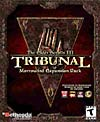
\includegraphics{media/image6.png} The Tribunal expansion for Morrowind
introduced a number of new functions and fixes and extends several of
the old ones. Note that both you and the user of the mod must have
Tribunal (or Bloodmoon, or GOTY edition) installed to make use of these,
so make sure you mark your mod accordingly. The functions are now sorted
into the main document, but this list may serve as an easy reference to
see which functions are Tribunal functions.

(Many thanks to Bethsoft's Mike Lipari for sharing the information on
these functions with the community.)

\hypertarget{changes-fixes-to-morrowind-scripting}{%
\subsubsection{Changes / fixes to Morrowind
scripting:}\label{changes-fixes-to-morrowind-scripting}}

\begin{itemize}
\item
  SetPos now accepts variables (float) as arguments.
\item
  SetAngle now accepts variables (float) as arguments.
\item
  Equip now works as intended and forces NPC to equip (put on) armor and
  clothing.
\item
  AIActivate was apparently fixed.
\end{itemize}

\hypertarget{index-of-new-tribunal-script-functions}{%
\subsubsection{Index of new Tribunal Script
Functions:}\label{index-of-new-tribunal-script-functions}}

\hypertarget{section-13}{%
\subsubsection{}\label{section-13}}

AddToLevCreature

AddToLevItem

ClearForceJump

ClearForceMoveJump

ClearForceRun

DaysPassed (variable)

DisableLevitation

EnableLevitation

ExplodeSpell

ForceJump

ForceMoveJump

ForceRun

GetArmorType

GetCollidingActor

GetCollidingPC

GetForceJump

GetForceMoveJump

GetForceRun

GetPCJumping

GetPCRunning

GetPCSneaking

GetScale

GetSpellReadied

GetSquareRoot

GetWaterLevel

GetWeaponDrawn

GetWeaponType

HasItemEquipped

HurtCollidingActor

ModScale

ModWaterLevel

PlaceItem

RemoveFromLevCreature

RemoveFromLevItem

SetDelete

SetJournalIndex (?)

SetScale

SetWaterLevel

\hypertarget{new-functions-that-come-with-bloodmoon}{%
\subsection{New functions that come with
BLOODMOON}\label{new-functions-that-come-with-bloodmoon}}

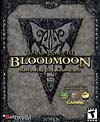
\includegraphics{media/image7.png} The second expansion for Morrowind,
Bloodmoon, introduces a few new functions. Note that both you and the
user of the mod must have Bloodmoon installed to make use of these, so
make sure you mark your mod accordingly.

\hypertarget{index-of-new-bloodmoon-script-functions-and-variables}{%
\subsubsection{Index of new Bloodmoon Script Functions and
variables:}\label{index-of-new-bloodmoon-script-functions-and-variables}}

AllowWereWolfForceGreeting

BecomeWerewolf

GetPCInJail

GetPCTraveling

GetWerewolfKills

IsWerewolf

PCKnownWerewolf

PlaceAtMe

SetWerewolfAcrobatics

TurnMoonRed

TurnMoonWhite

UndoWerewolf

\hypertarget{previously-undocumented-functions}{%
\subsection{\texorpdfstring{\hfill\break
Previously undocumented
functions}{ Previously undocumented functions}}\label{previously-undocumented-functions}}

These functions were not documented in the original helpfile. I have
explained most of them in this guide, but for a few the uses are still
unknown to me. I thought it might be useful to have as a list for an
easy overview. The list was put together by someone who Hex-edited the
TES-CS .exe, so it's likely to be complete.

(thanks to Soralis for the list and XPCagey and others who helped to put
it together):

\textbf{Undocumented in Helpfile:}

PayFineThief

EnableStatReviewMenu

GetFactionReaction

ShowMap

EnableBirthMenu

EnableClassMenu

EnableRaceMenu

EnableNameMenu

RemoveEffects

EnableMagicMenu

EnableMapMenu

EnableInventoryMenu

EnableStatsMenu

GetInterior

GetLineOfSight (alias for GetLOS)

GetWindSpeed

GetCurrentTime

ResetActors

OutputRefInfo

MenuTest

Functions which are \textbf{spelled differently than documented
(XPCagey):}

getHealthRatio -\textgreater{} getHealthGetRatio

getInvisible -\textgreater{} getInvisibile

setInvisible -\textgreater{} setInvisibile

modInvisible -\textgreater{} modInvisibile

getSecundusPhase -\textgreater{} getSecundaPhase

\textbf{(actual syntax on the right)}

And those which don't work:

getPlayerViewSwitch -\textgreater{} (can't be used)

OnRepair -\textgreater{} not in string tables

UsedOnMe -\textgreater{} not in string tables

name -\textgreater{} not in string tables

Also be aware that most console commands can be compiled as functions by
the Construction Set (see list below). These are also to a large part
not listed by the helpfile.

\hypertarget{variable-type-functions}{%
\subsection{\texorpdfstring{\hfill\break
Variable-type
functions:}{ Variable-type functions:}}\label{variable-type-functions}}

For easy reference, the following list shows all those variable/function
type hybrids that you \textbf{need to declare} as variables if you use
them in a script.

\hypertarget{local-variables-that-get-set-by-the-game}{%
\subsubsection{Local variables that get set by the
game:}\label{local-variables-that-get-set-by-the-game}}

Short OnPCEquip

Short OnPCAdd

Short OnPCRepair

Short OnPCSoulGemUse

Short OnPCHitMe

Float minimumProfit (Tribunal)

\hypertarget{local-variables-that-you-can-set-as-a-flag}{%
\subsubsection{Local variables that you can set as a
flag:}\label{local-variables-that-you-can-set-as-a-flag}}

Short Companion (Tribunal)

Short StayOutside (Tribunal)

Short PCSkipEquip

\hypertarget{special-globals}{%
\subsubsection{Special Globals}\label{special-globals}}

Some globals hold special significance that you can take advantage of
for your own scripting. Since they are globals, you do not need to
declare them.

\begin{longtable}[]{@{}
  >{\raggedright\arraybackslash}p{(\columnwidth - 2\tabcolsep) * \real{0.36}}
  >{\raggedright\arraybackslash}p{(\columnwidth - 2\tabcolsep) * \real{0.64}}@{}}
\toprule
\endhead
Short NPCVoiceDistance (750) & Used as a distance when Following NPCs
call after you to wait for them (e.g. see DandsaScript) \\
Float GameHour & Holds the current hour of the day (0-23)

Note, this is a float, so 10:30 would be represented as 10.5. See the
section on float variables for more information \\
Short Day & Holds the current day of the month (1-30) \\
Short Month & Holds the current Month of the year (0-11) \\
Short Year (427) & Holds the current year \\
Float TimeScale (30) & Sets the ratio of real-time/game-time \\
Short Random100 & Is randomly set between 0-100 (set by main script when
out of menumode) \\
Short PCRace & Contains the player's Race

(1=Argonian, 2=Breton, 3=Dark Elf, 4=High Elf, 5=Imperial, 6= Khajiit,
7=Nord, 8=Orc, 9=Redguard, 10=Woodelf)

If the player is using a custom race, PCRace will remain 0 by default.
Note that it is possible to add your own racecheck script for custom
races, and set PCRace to a custom value, but be warned: if two mods do
this, you may have conflicts. As this variable is only used in dialog,
it is not required that you set it to a different number for every
custom race you make. If you made a new race with dialog, instead of
using this it would be far better to make your own global variable as it
would be less likely to conflict with other mods. \\
Short PCVampire & Vampire status: 0=Normal, 1=Vampire, -1= cured \\
Short VampClan & If the PC becomes a vampire, this indicates his clan.
1=Aundae, 2=Berne, 3=Quarra \\
Short DaysPassed & Contains the number of days since the game started.
Requires an explicit declaration, which is present in Tribunal but must
otherwise be added (not present in Bloodmoon or Morrowind). \\
Short PCWerewolf & Werewolf status: 0=Normal, 1=Werewolf, -1=Cured \\
Float WerewolfClawMult (25.00) & Increased during the Werewolf quests to
make your claw attack more powerful. \\
Short PCHasGoldDiscount & Used in dialogue. Gets set to 1 if player has
enough gold to pay thieves guild discount on the "price on your
head". \\
Short PCHAsTurnIn & Used in dialogue. Gets set to 1 if player has enough
gold to pay the reduced fee for turning yourself in. \\
Short PCHasCrimeGold & Used in dialogue. Gets set to 1 if player has
enough gold to pay the crime fee. \\
Short CrimeGoldTurnIn & Gold needed for reduced crime fee \\
CrimeGoldDiscount & Gold needed for thieves guild discount crime fee \\
\bottomrule
\end{longtable}

\hypertarget{game-units}{%
\subsection{\texorpdfstring{\hfill\break
Game units:}{ Game units:}}\label{game-units}}

1 game unit = 0.56 inches\\
50 =28 inches\\
500 = 23.3 feet\\
5000 = 233.3 feet\\
8192 = 385 feet = 1 game cell

1 game unit = 1.42 cm\\
100 game units = 142 cm = 1.42 meters\\
1000 game units = 14.2 meters\\
8192 game units = 116.33 meters = 1 exterior cell

The island of Morrowind itself is 5.00 km north to south and 4.65 km
east to west.

(thanks to Iudas for this information)

\hypertarget{derived-attribute-calculations}{%
\subsection{Derived attribute
calculations:}\label{derived-attribute-calculations}}

(Thanks to DinkumThinkum for this info.)

The following is based on how they're calculated for player characters;
checking in the Construction Set, NPC derived attributes appear to use
basically the same system (if auto-calculate is enabled).

\textbf{Maximum Fatigue:} equals the total of current Strength, current
Endurance, current Willpower, and current Agility.

\textbf{Maximum Magicka:} current Intelligence times the character's
magicka multiplier (varies with race and birthsign). For NPCs, the
multiplier apparently is fixed at two (default value of
fNPCbaseMagickaMult: see Game Settings); race doesn't seem to affect it.

NOTE: this is based on the Maximum Magicka shown in the editor. Racial
abilities that fortify Maximum Magicka are listed in the 'spells'
section of the NPC's properties page, so that may be figured into the
maximum value used during game play; haven't tested this.

\textbf{Maximum Encumbrance:} five times the character's current
Strength.

\textbf{Maximum Health (player):} When you create your character, their
starting maximum Health (at first level) is one half the total of their
Strength and Endurance. After that, each time your character goes up a
level their maximum Health is increased by 10\% of their Endurance
(value set by fLevelUpHealthEndMult, see Game Settings). This is based
on the character's base natural Endurance; magical modifications to
Endurance are ignored.

Strength is only used to calculate the player character's starting value
for maximum Health; it has no further affect on Health once the
character has been created. Also, Endurance affects the amount added to
the character's maximum Health each level; there's no recalculation of
the amount added in previous levels.

\textbf{Maximum Health (NPCs):} A number of formulas for NPC health have
been proposed, but I (melian) have yet to find one that works for more
than one NPC. At base level, NPC Health appears to be auto-calculated in
the same way as the player's: (STR + END)/2. After that it gets tricky,
and most formulas fail quite dramatically at higher levels.

For \emph{some} NPCs: The calculation is based on the character's
Strength and Endurance, and Health increase factor per level is constant
within three brackets: before STR has maxed (largest increase), after
STR but before END has maxed (smaller increase), and after both have
maxed (constant smaller increase from then on). It's usually easy enough
to calculate a single NPC's Health at any given level by noting Health,
Strength and Endurance at various levels and working out the increase
factor per level in each of the three brackets (remembering that values
are really floats: averaging a larger value will get a more accurate
increase factor). This has worked for most NPCs I've used it on, whose
Strength maxed well before Endurance did. I'm not sure of the
progression for NPCs whose Endurance maxes first, and race may have
something to do with it as well.\protect\hypertarget{_Toc53412751}{}{}

\hypertarget{magic-effect-list}{%
\subsection{Magic Effect List}\label{magic-effect-list}}

For the function GetEffect, you need the ID-string itself (e.g.
GetEffect sEffectWaterBreathing). For the RemoveEffects function, the
effect number is used (e.g. RemoveEffects, 0)

0 =\textgreater{} sEffectWaterBreathing\\
1 =\textgreater{} sEffectSwiftSwim\\
2 =\textgreater{} sEffectWaterWalking\\
3 =\textgreater{} sEffectShield\\
4 =\textgreater{} sEffectFireShield\\
5 =\textgreater{} sEffectLightningShield\\
6 =\textgreater{} sEffectFrostShield\\
7 =\textgreater{} sEffectBurden\\
8 =\textgreater{} sEffectFeather\\
9 =\textgreater{} sEffectJump\\
10 =\textgreater{} sEffectLevitate\\
11 =\textgreater{} sEffectSlowFall\\
12 =\textgreater{} sEffectLock\\
13 =\textgreater{} sEffectOpen\\
14 =\textgreater{} sEffectFireDamage\\
15 =\textgreater{} sEffectShockDamage\\
16 =\textgreater{} sEffectFrostDamage\\
17 =\textgreater{} sEffectDrainAttribute\\
18 =\textgreater{} sEffectDrainHealth\\
19 =\textgreater{} sEffectDrainSpellpoints\\
20 =\textgreater{} sEffectDrainFatigue\\
21 =\textgreater{} sEffectDrainSkill\\
22 =\textgreater{} sEffectDamageAttribute\\
23 =\textgreater{} sEffectDamageHealth\\
24 =\textgreater{} sEffectDamageMagicka\\
25 =\textgreater{} sEffectDamageFatigue\\
26 =\textgreater{} sEffectDamageSkill\\
27 =\textgreater{} sEffectPoison\\
28 =\textgreater{} sEffectWeaknessToFire\\
29 =\textgreater{} sEffectWeaknessToFrost\\
30 =\textgreater{} sEffectWeaknessToShock\\
31 =\textgreater{} sEffectWeaknessToMagicka\\
32 =\textgreater{} sEffectWeaknessToCommonDisease\\
33 =\textgreater{} sEffectWeaknessToBlightDisease\\
34 =\textgreater{} sEffectWeaknessToCorprusDisease\\
35 =\textgreater{} sEffectWeaknessToPoison\\
36 =\textgreater{} sEffectWeaknessToNormalWeapons\\
37 =\textgreater{} sEffectDisintegrateWeapon\\
38 =\textgreater{} sEffectDisintegrateArmor\\
39 =\textgreater{} sEffectInvisibility\\
40 =\textgreater{} sEffectChameleon\\
41 =\textgreater{} sEffectLight\\
42 =\textgreater{} sEffectSanctuary\\
43 =\textgreater{} sEffectNightEye\\
44 =\textgreater{} sEffectCharm\\
45 =\textgreater{} sEffectParalyze\\
46 =\textgreater{} sEffectSilence\\
47 =\textgreater{} sEffectBlind\\
48 =\textgreater{} sEffectSound\\
49 =\textgreater{} sEffectCalmHumanoid\\
50 =\textgreater{} sEffectCalmCreature\\
51 =\textgreater{} sEffectFrenzyHumanoid\\
52 =\textgreater{} sEffectFrenzyCreature\\
53 =\textgreater{} sEffectDemoralizeHumanoid\\
54 =\textgreater{} sEffectDemoralizeCreature\\
55 =\textgreater{} sEffectRallyHumanoid\\
56 =\textgreater{} sEffectRallyCreature\\
57 =\textgreater{} sEffectDispel\\
58 =\textgreater{} sEffectSoultrap\\
59 =\textgreater{} sEffectTelekinesis\\
60 =\textgreater{} sEffectMark\\
61 =\textgreater{} sEffectRecall\\
62 =\textgreater{} sEffectDivineIntervention\\
63 =\textgreater{} sEffectAlmsiviIntervention\\
64 =\textgreater{} sEffectDetectAnimal\\
65 =\textgreater{} sEffectDetectEnchantment\\
66 =\textgreater{} sEffectDetectKey\\
67 =\textgreater{} sEffectSpellAbsorption\\
68 =\textgreater{} sEffectReflect\\
69 =\textgreater{} sEffectCureCommonDisease\\
70 =\textgreater{} sEffectCureBlightDisease\\
71 =\textgreater{} sEffectCureCorprusDisease\\
72 =\textgreater{} sEffectCurePoison\\
73 =\textgreater{} sEffectCureParalyzation\\
74 =\textgreater{} sEffectRestoreAttribute\\
75 =\textgreater{} sEffectRestoreHealth\\
76 =\textgreater{} sEffectRestoreSpellPoints\\
77 =\textgreater{} sEffectRestoreFatigue\\
78 =\textgreater{} sEffectRestoreSkill\\
79 =\textgreater{} sEffectFortifyAttribute\\
80 =\textgreater{} sEffectFortifyHealth\\
81 =\textgreater{} sEffectFortifySpellpoints\\
82 =\textgreater{} sEffectFortifyFatigue\\
83 =\textgreater{} sEffectFortifySkill\\
84 =\textgreater{} sEffectFortifyMagickaMultiplier\\
85 =\textgreater{} sEffectAbsorbAttribute\\
86 =\textgreater{} sEffectAbsorbHealth\\
87 =\textgreater{} sEffectAbsorbSpellPoints\\
88 =\textgreater{} sEffectAbsorbFatigue\\
89 =\textgreater{} sEffectAbsorbSkill\\
90 =\textgreater{} sEffectResistFire\\
91 =\textgreater{} sEffectResistFrost\\
92 =\textgreater{} sEffectResistShock\\
93 =\textgreater{} sEffectResistMagicka\\
94 =\textgreater{} sEffectResistCommonDisease\\
95 =\textgreater{} sEffectResistBlightDisease\\
96 =\textgreater{} sEffectResistCorprusDisease\\
97 =\textgreater{} sEffectResistPoison\\
98 =\textgreater{} sEffectResistNormalWeapons\\
99 =\textgreater{} sEffectResistParalysis\\
100 =\textgreater{} sEffectRemoveCurse\\
101 =\textgreater{} sEffectTurnUndead\\
102 =\textgreater{} sEffectSummonScamp\\
103 =\textgreater{} sEffectSummonClannfear\\
104 =\textgreater{} sEffectSummonDaedroth\\
105 =\textgreater{} sEffectSummonDremora\\
106 =\textgreater{} sEffectSummonAncestralGhost\\
107 =\textgreater{} sEffectSummonSkeletalMinion\\
108 =\textgreater{} sEffectSummonLeastBonewalker\\
109 =\textgreater{} sEffectSummonGreaterBonewalker\\
110 =\textgreater{} sEffectSummonBonelord\\
111 =\textgreater{} sEffectSummonWingedTwilight\\
112 =\textgreater{} sEffectSummonHunger\\
113 =\textgreater{} sEffectSummonGoldensaint\\
114 =\textgreater{} sEffectSummonFlameAtronach\\
115 =\textgreater{} sEffectSummonFrostAtronach\\
116 =\textgreater{} sEffectSummonStormAtronach\\
117 =\textgreater{} sEffectFortifyAttackBonus\\
118 =\textgreater{} sEffectCommandCreatures\\
119 =\textgreater{} sEffectCommandHumanoids\\
120 =\textgreater{} sEffectBoundDagger\\
121 =\textgreater{} sEffectBoundLongsword\\
122 =\textgreater{} sEffectBoundMace\\
123 =\textgreater{} sEffectBoundBattleAxe\\
124 =\textgreater{} sEffectBoundSpear\\
125 =\textgreater{} sEffectBoundLongbow\\
126 =\textgreater{} sEffectExtraSpell\\
127 =\textgreater{} sEffectBoundCuirass\\
128 =\textgreater{} sEffectBoundHelm\\
129 =\textgreater{} sEffectBoundBoots\\
130 =\textgreater{} sEffectBoundShield\\
131 =\textgreater{} sEffectBoundGloves\\
132 =\textgreater{} sEffectCorpus\\
133 =\textgreater{} sEffectVampirism\\
134 =\textgreater{} sEffectSummonCenturionSphere\\
135 =\textgreater{} sEffectSunDamage\\
136 =\textgreater{} sEffectStuntedMagicka

\hypertarget{list-of-console-commands}{%
\subsection{\texorpdfstring{\hfill\break
List of console
commands}{ List of console commands}}\label{list-of-console-commands}}

Console (in game only commands). Most are useful for debugging / testing
only, but some of these (marked with *) CAN be used in scripts. For
functions that produce an output to console: you can continue playing
with the console open by rightclicking outside of the console window.

\begin{longtable}[]{@{}
  >{\raggedright\arraybackslash}p{(\columnwidth - 4\tabcolsep) * \real{0.30}}
  >{\raggedright\arraybackslash}p{(\columnwidth - 4\tabcolsep) * \real{0.12}}
  >{\raggedright\arraybackslash}p{(\columnwidth - 4\tabcolsep) * \real{0.58}}@{}}
\toprule
\begin{minipage}[b]{\linewidth}\raggedright
\textbf{Command}
\end{minipage} & \begin{minipage}[b]{\linewidth}\raggedright
\textbf{short}
\end{minipage} & \begin{minipage}[b]{\linewidth}\raggedright
\textbf{Description}
\end{minipage} \\
\midrule
\endhead
\textsuperscript{*}CenterOnCell, "\emph{Cell\_ID"} & COC & Places the PC
in the named cell. Very useful for testing mods. \\
\textsuperscript{*}CenterOnExterior, \emph{X, Y} & COE & Places the PC
in the exterior cell grid. \\
CreateMaps \emph{"Filename.esp"} & & Creates map image file depending on
the Create Maps Enable value in the Morrowind.INI file. If it is 1
(XBox), the file FILENAME.ESP.MAP is created in the DataFiles path with
the map data (unknown format). If the value is 2 (Exterior Cell Maps)
and you have created a directory /Maps/ in the main Morrowind game
directory, this command will create a 256x256 high color bitmap of each
exterior cell in the game. This command takes a long while even on fast
computers as each cell in the game is loaded.

Note that CreateMaps won't generate an image of the cell in which the
player is currently located. So if you're standing in your mod's
landscape, all the cells around it are processed just fine, but you'll
be missing the current cell. To work around this, move to a cell you
don't care about before starting the CreateMaps process. You might also
be able to move to an interior cell, but this is untested. -(Klinn) \\
& BC & \begin{minipage}[t]{\linewidth}\raggedright
Beta Comment: Edit the morrowind.ini file to give a filename in the beta
comment line:\\
Beta Comment File=BetaComment.txt\\
Then you can use the BC Command to make a note about an object in the
game. You open the console and click something, then type your comment,
like this:\\
BC "Root not attached well."\\
And in BetaComment.txt you get:\\
6/20/2004 (21:02) Morrowind.esm 5/8/2003 (21:07) Paul ex\_t\_root\_03
Tel Vos (10,14) 85078 118468 4111 "Root not attached well."\\
The time I made the comment, the file the object is from, the
modification time of that file, my name (windows log-in), the cell, the
X, Y and Z Position of the object, and of course, the comment (forum
info / ManaUser).\strut
\end{minipage} \\
FillJournal & & add all entries to journal, takes a long time \\
\textsuperscript{*}FillMap & & show all the towns / uniquely named cells
on the full map. Takes a few seconds. Not recommended for scripts. \\
\textsuperscript{*}FixMe & & Jump 128 units away from where I am now.
Good to get "unstuck" \\
GetFactionReaction, \emph{"factionID", "factionID", amount} & & The
faction ID's are not optional, works in Console window only. Not sure
about the actual meaning of the output. \\
Help & & Lists, and shows shorthand for most commands \\
MoveOneToOne & MOTO & This command changes the speed at which the PC
actor (and presumably other actors) RUN. With MOTO active your walking
and running speeds are the same, and the same animation will play for
either walking or running.(IndigoRage) \\
ObjectReferenceInfo & ORI & Lists info about the selected object, such
as the cell it's in and the esm/esp file it originates from. Handy when
identifying which mod added a certain item. \\
OutputObjCounts & & Counts all objects in various categories. Output is
written to the console window \\
OutputRefCounts & & Counts all references in various categories. Output
is written to the console window. \\
& PT & "Purge textures" makes the engine reload all textures. If you
play in windows mode you can use this to test textures in-game, while
editing them in another application. \\
Show \emph{global\_var} & & Writes the value of the specified global
variable to the console \\
ShowVars & SV & Lists global variables and variables in global scripts,
or local variables if you click on an object with a local script first.
Output to console. \\
StopCellTest & SCT & Stops the cell test, player remains in currently
loaded cell \\
TestCells & & Loads all cells in alphabetical order (On testing it
seemed to be only interiors - Not sure about difference to
TestInteriorCells)

Note: TestCells, TestInteriorCells and TestThreadCells is a bit buggy.
Even if you load a savegame while it's in process, it will continue
until the last cell is reached. \\
TestInteriorCells & & Loads all interior cells in alphabetical order \\
TestThreadCells & & \begin{minipage}[t]{\linewidth}\raggedright
Loads all exterior cells , then all interior cells. Exterior cells load
in the following order:

{[}biggest x number{]}, {[}biggest y number{]}\\
{[}biggest x number{]}, {[}biggest y number - 1{]}\\
When the "y" number reaches the last value this follows\\
{[}biggest x number - 3 \_OR\_ - 1{]}, {[}biggest y number{]}\\
{[}biggest x number - 3 \_OR\_ - 1{]}, {[}biggest y number - 1{]}\\
etc.

Interior cells load in alphabetical order.

The command pauses in menumode, but not exactly when the menumode is
first triggered. It waits several frames. -(unknown)\strut
\end{minipage} \\
TestModels & T3D & Test all objects and reports missing .nif files \\
\textsuperscript{*}ToggleAI & TA & Stops AI, including combat. Useful in
testing a cell without being attacked by nasties \\
ToggleBorders~ & TB & Shows borders of exterior cells \\
ToggleCombatStats & TCS & Allows you to monitor combat statistics in
realtime. Enable this, then right-click outside the console window to
continue playing with the console window open. Note: When I tested, the
output was also written to log.txt - not sure if this is by default. \\
\textsuperscript{*}ToggleCollision & TCL & Turns collision on and off.
Lets you float through walls. Can make Actors drop through floors, or
float \\
ToggleCollisionBoxes & TCB & Shows the collision boxes of all models \\
ToggleCollisionGrid & TCG & Outputs a matrix to the screen that probably
indicates the current collision situation - I couldn't interpret it.
Slows the game to a crawl \\
ToggleDebugText & TDT & Displays some debugging info on the screen:
Players animation groups, speed, heading, position, FPS, delta movement
per frame, and some I could not identify \\
ToggleDialogueStats & TDS & Outputs result of persuasion attempts (and
maybe other dialogue results?) to the console \\
\textsuperscript{*}ToggleFogOfWar & TFOW & Lets you see all of the local
map \\
ToggleFullHelp & TFH & Shows you ownership and script on mouseover while
in console mode or in the info box during normal play. Also displays
info on how the game fills leveled lists (upon entering a cell or
opening a container) in the console. \\
\textsuperscript{*}ToggleGodMode & TGM & Makes you invulnerable. \\
ToggleGrid & TG & Displays the current cell's coordinates, and a grid of
the currently loaded cells on screen, indicating the activities of
morrowinds "thread loading" (caching of cells) \\
ToggleKillStats & TKS & When an actor is killed the name of the kill,
the total number of kills, and (with Bloodmoon) werewolf kills, is
displayed in the console \\
ToggleLights & & Unknown, I did not get any effect or output from
this. \\
ToggleLoadFade & & Unknown. From the name it would seem to refer to the
screen fading in and out on loading of a game or teleporting, but I
could not detect a difference. \\
ToggleMagicStats & TMS & Displays info on active spell effects in the
console. Gives effect \#, spell name, and statistical info \\
\textsuperscript{*}ToggleMenus & TM & Disables all menus (including the
main save/load/options menu!). Menus stay invisible until console is
brought up again (press console key twice). Not recommended for use in
scripts - If the player uses the console, your script may end up
disabling the menus completely! \\
ToggleScripts & & Presumably stops script processing \\
ToggleScriptOutput & TSO & Unknown, I did not get any effect or output
from this. \\
ToggleStats & TST & Activates all stat debugging modes
(ToggleCombatStats, ToggleMagicStats, ToggleDialogueStats,
ToggleKillStats) \\
\textsuperscript{*}ToggleSky & TS & Switches the sky off. Also affects
lighting, basically with switched off sky it's also "night". \\
ToggleTextureString & TTS & Unknown, I did not get any effect or output
from this. \\
ToggleWater & & Unknown, I did not get any effect or output from
this. \\
\textsuperscript{*}ToggleWorld & TW & Stops the "world" and all objects
from being rendered, just leaves the sky and water. Does not affect
anything else, meaning collision, AI, etc. All remain active, just
invisible \\
ToggleWireframe & TWF & Shows grid instead of full render \\
TogglePathGrid & TPG & Toggle AI path grid display \\
\textsuperscript{*}ToggleVanityMode & TVM & Switches to vanity mode,
player can not switch again until toggle is off. May be useful for
cutscenes. \\
& SA & "Show Animation" Shows status and animation info for the selected
actor: Spell readied, weapon drawn, attacked, animation group \\
ShowGroup & SG & Writes the selected Actors goup actual ID + reference
number to the console window. For the player this is PlayerSaveGame \\
& ST & "Show target group" Writes the ID + reference number of the
selected actors "target" group (combat opponent) to the console
window. \\
ShowScenegraph & SSG & Opens a new window that displays a hierarchical
view of (I assume) the data structure of the currently rendered scene.
Use TAB to get to the window. MW will remain unresponsive while the
scene graph window is open. \\
\bottomrule
\end{longtable}

\hypertarget{game-settings}{%
\subsection{\texorpdfstring{\hfill\break
Game Settings}{ Game Settings}}\label{game-settings}}

The following long table is a list of game settings. Listed here are all
settings that have a numerical value. Not listed are string entries --
which are used to set many standard message texts, menu-texts, spell
effect names, etc. But since they are fairly descriptive, they should be
easy to figure out. Not so the numerical settings. Thanks to four forum
members (maxpublic, Ldones, Wakim and Iudas), the meaning of many of the
settings is now known and compiled into the list below. The list may
still be a bit rough. I have not edited it thoroughly, but I am sure it
will be interesting information for many modders.

In many cases where you see Base and Mult game settings, the formula
they're involved in is a standard linear equation in the form y = mx +
b, where m is the mult, b is the base, and x is some attribute, skill,
or other value.

Note that the entry names begin with f or i (for floats and integers).
The string entries begin with s (string). To my knowledge they can not
be changed in-game, only in the TES-CS.

\begin{longtable}[]{@{}
  >{\raggedright\arraybackslash}p{(\columnwidth - 6\tabcolsep) * \real{0.07}}
  >{\raggedright\arraybackslash}p{(\columnwidth - 6\tabcolsep) * \real{0.27}}
  >{\raggedright\arraybackslash}p{(\columnwidth - 6\tabcolsep) * \real{0.09}}
  >{\raggedright\arraybackslash}p{(\columnwidth - 6\tabcolsep) * \real{0.58}}@{}}
\toprule
\endhead
\textbf{Nr.} & \textbf{Name} & \textbf{Value} & \textbf{Description and
Comments} \\
"465" & "fRepairMult" & 1.0000 & Sets the general effectiveness of the
repair skill of the character, via the armorer's hammer used \\
"466" & "fRepairAmountMult" & 3.0000 & Tells the game how many points of
health are returned to the item when repaired

Determines cost for repairing items (Whether calculated from Max Item
Health or Item Cost, I'm not sure) \\
"467" & "fSpellValueMult" & 10.0000 & \\
"468" & "fSpellMakingValueMult" & 7.0000 & \\
"469" & "fEnchantmentValueMult" & 1000.0000 & The setting for the price
you pay at an enchanter to enchant an item. Linear. \\
"470" & "fTravelMult" & 4000.0000 & Sets the cost of Silt Strider and
boat travel (I think)

Multiplies cost of Travel -- Unsure why the number is so high, but
raising it raises the cost of Fast Travel \\
"471" & "fTravelTimeMult" & 16000.0000 & Tells the game how much time
elapses during this sort of travel \\
"472" & "fMagesGuildTravel" & 10.0000 & Sets the cost of Guild Guide
travel \\
& & & \\
"947" & "fWortChanceValue" & 15.0000 & Is compared to your alchemy skill
to determine which of the effects of an ingredient you can see. -(Wakim,
Iudas) \\
& & & \\
"949" & "fMinWalkSpeed" & 100.0000 & This is the minimum walking speed
of the PC, regardless of stats, skills or encumbrance \\
"950" & "fMaxWalkSpeed" & 200.0000 & This is the maximum walking speed
of the PC, regardless of stats, skills, or encumbrance

The actual walking speed of NPC's (and the PC) is set by checking
various factors (Speed, Athletics, etc.) and assigning a value between
fMinWalkSpeed and fMaxWalkSpeed based on that -- The two settings
dictate the spectrum of Walk Speeds \\
"951" & "fMinWalkSpeedCreature" & 5.0000 & The same as for the PC, but
if you badly encumber a creature it'll move veeerrry slowly. I've done
this by accident. \\
"952" & "fMaxWalkSpeedCreature" & 300.0000 & Same as above, they get
faster, so they cover the speed spectrum more rapidly \\
"953" & "fEncumberedMoveEffect" & 0.3000 & This sets how encumbrance
affects walking and running speed, within the min/max limits set by
other values. \\
"954" & "fBaseRunMultiplier" & 1.7500 & Exactly as it says. Changing the
value will increase/decrease base running speed.

Dictates how much faster Running is than the current Walk Speed \\
"955" & "fAthleticsRunBonus" & 1.0000 & Sets how Athletics affects
running speed. \\
"956" & "fJumpAcrobaticsBase" & 128.0000 & Sets the base jumping
distance for the PC. \\
"957" & "fJumpAcroMultiplier" & 4.0000 & Sets the multiplier for
Acrobatics, which is why you can leap over tall buildings when your Acro
is high enough. \\
"958" & "fJumpEncumbranceBase" & 0.5000 & Effects how greatly jumping
ability is effected by Encumbrance, but I'm unsure how \\
"959" & "fJumpEncumbranceMultiplier" & 1.0000 & Effects how greatly
jumping ability is effected by Encumbrance, but I'm unsure how \\
"960" & "fJumpRunMultiplier" & 1.0000 & UNSURE -- Presumably effects
Jump Distance while running (it doesn't seem to effect height, but I
could be wrong) \\
"961" & "fJumpMoveBase" & 0.5000 & \\
"962" & "fJumpMoveMult" & 0.5000 & \\
"963" & "fSwimWalkBase" & 0.5000 & Multiplies your walking speed to
achieve the swimming speed at a 'walk'

Base swim speed while `walking' \\
"964" & "fSwimRunBase" & 0.5000 & Multiplies your running speed to
achieve the swimming speed at a 'run'. \\
"965" & "fSwimWalkAthleticsMult" & 0.0200 & Tells the game how Athletics
affects 'walking' swimming speed. These low values keep you from flying
through the water like you do on land when your Athletics is high. \\
"966" & "fSwimRunAthleticsMult" & 0.1000 & Same as above. \\
"967" & "fSwimHeightScale" & 0.9000 & Determines how close to the
surface you have to be before the breathe indicator goes away \\
"968" & "fHoldBreathTime" & 20.0000 & The number of seconds your PC can
hold her breath.

Base time that a character can remain underwater before incurring
suffocation damage \\
"969" & "fHoldBreathEndMult" & 0.5000 & How Endurance affects the time
you can hold your breath. I believe this is a flat-out multiplier to
End, added as seconds to HoldBreathTime.\textless Doesn't seem to
work.\textgreater{} \\
"970" & "fSuffocationDamage" & 3.0000 & The amount of health damage you
take each second you suffocate \\
"971" & "fMinFlySpeed" & 5.0000 & Exactly as it says -- minimum flying
speed. \\
"972" & "fMaxFlySpeed" & 300.0000 & See above \\
"973" & "fStromWindSpeed" & 0.7000 & UNSURE - Determines altered walk
speed during an ash or blight storm, but I'm unsure how -- Might be a
separate value from that entirely -- might determine speed of storm
particles /sprites(Dust, etc.) Interesting (possibally related) note,
while treading water in an ash storm, I noticed I was moving
slightly. \\
"974" & "fStromWalkMult" & 0.2500 & Determines altered walk speed during
an ash or blight storm, but I'm unsure how uses the getwindspeed to
lower the PC movement speed during storms... \\
"975" & "fFallDamageDistanceMin" & 400.0000 & The minimum distance you
have to fall before you take damage.

(Presumably in units) In game units each unit - .0.56 inches \\
"976" & "fFallDistanceBase" & 0.0000 & This will increase/decrease the
distance needed to fall before you take damage. \\
"977" & "fFallDistanceMult" & 0.0700 & Higher you are the more damage
you take when you hit \\
"978" & "fFallAcroBase" & 0.2500 & Acrobatics skill increases the
distance you can fall before you take damage. \\
"979" & "fFallAcroMult" & 0.0100 & Has to do w/ how the Acrobatics skill
effects Fall Distance and Damage, but unsure how \\
"980" & "iMaxActivateDist" & 192 & Maximum distance for the player to be
able to `Activate' an object - approx 9 feet \\
"981" & "iMaxInfoDist" & 192 & Maximum distance for an Info message
(object/NPC/creature name, etc.) to pop up in the Player's view \\
"982" & "fVanityDelay" & 30.0000 & Seconds until VanityMode begins --
the camera starts circling the player if there is no input via mouse or
keyboard. \\
"983" & "fMaxHeadTrackDistance" & 400.0000 & IIRC, this is the maximum
distance an NPC or creature can be away from another NPC or creature and
still trigger the 'head follow' routine you sometimes see. Put your PC
in Balmora, let it go to Vanity View and you'll see your PC watch
passing NPCs and 'follow' their movements for a certain amount of
time. \\
"984" & "fInteriorHeadTrackMult" & 0.5000 & UNSURE -- something to do w/
the modifier for this in Interiors -- Do they track at half-distance in
Interiors? \\
"985" & "iHelmWeight" & 5 & \multirow{7}{*}{These values are used to set
what weights are used to determine whether a piece of armor is light,
medium, or heavy. Altering a value alters these categories for *all*
armor of that type *everywhere* in the game. Rather nice, actually; I
used it in redux to set weight categories for all of my armor types
across the board.} \\
"986" & "iPauldronWeight" & 10 \\
"987" & "iCuirassWeight" & 30 \\
"988" & "iGauntletWeight" & 5 \\
"989" & "iGreavesWeight" & 15 \\
"990" & "iBootsWeight" & 20 \\
"991" & "iShieldWeight" & 15 \\
"992" & "fLightMaxMod" & 0.6000 & \multirow{2}{*}{These values are used
in conjunction with armor weights to set the weight classes (Light,
Medium, Heavy).} \\
"993" & "fMedMaxMod" & 0.9000 \\
"994" & "fUnarmoredBase1" & 0.1000 & \multirow{2}{*}{These two values
dictate the range of AR for characters going Unarmored, based on the
Unarmored skill -- As they are, the settings produce a Maximum Unarmored
AR of 65 (at 100 Unarmored skill), which you can see is some for of
multiplication between the two settings -- Reversing the values produces
the same effect , so it seems the values are interchangeable (unless I
missed something -- could be wrong) - Changing one to 1.000 and the
other to 0.0650 results in a max Unarmored AR of 650 -- The game
multiplies the numbers and then multiplies the resulting number by 1000
to obtain the actual in-game Max Unarmored AR -- Doesn't seem to effect
Min AR independently, only max - Progression of AR (from low skill to
high skill) appears to be hard-coded.

It has also been found that the Unarmored skill doesn't work at all
UNLESS atleast one item of armor is worn. (Forum Info / The other
Felix)} \\
"995" & "fUnarmoredBase2" & 0.0650 \\
"996" & "iBaseArmorSkill" & 30 & The Skill Level where in-game armors
reach their base (i.e. `In-Editor') AR value -- Example: Glass Armor has
a Base AR of 50 -- At Light Armor skill level 30 (as indicated above),
it will read as having AR 50 in-game -- Before Skill Level 30, armors
have diminished AR's from their Base Value, and after Skill Level 30,
armors have higher AR's than their base until Skill Level reaches 100 --
I haven't figured out the game's scheme for determining the mult value
yet \\
"997" & "fBlockStillBonus" & 1.2500 & UNSURE -- Presumably the amount
that standing still increases the chance to block \\
"998" & "fDamageStrengthBase" & 0.5000 & Your STR adds to the damage you
do with weapons. This determines how much damage is added. \\
"999" & "fDamageStrengthMult" & 0.1000 & Effects amount that Strength
effects damage dealt in combat (Unsure of how this value relates to
in-game effect) \\
"1000" & "fSwingBlockBase" & 1.0000 & \\
"1001" & "fSwingBlockMult" & 1.0000 & \\
"1002" & "fFatigueBase" & 1.2500 & How much fatigue you lose while
walking. However, this appears to let you jump very high without getting
hurt (Bug? -- Forum Info / DinkumThinkum).

1002 -- 1022 All effect `Fatigue' in-game, obviously -- For separate
actions, although not all of them actually have an effect in-game (I've
never been able to get spells to reduce fatigue) -- They seem pretty
self-explanatory, but I haven't tested them thoroughly \\
"1003" & "fFatigueMult" & 0.5000 & Used to determine successful chance
of casting if you are fatigued \\
"1004" & "fFatigueReturnBase" & 2.5000 & How much fatigue you regain per
second. This is why you don't actually fatigue while walking. \\
"1005" & "fFatigueReturnMult" & 0.0200 & How much fatigue returns per
second while walking \\
"1006" & "fEndFatigueMult" & 0.0400 & \\
"1007" & "fFatigueAttackBase" & 2.0000 & How much fatigue you lose with
every melee attack you make \\
"1008" & "fFatigueAttackMult" & 0.0000 & \\
"1009" & "fWeaponFatigueMult" & 0.2500 & \\
"1010" & "fFatigueBlockBase" & 4.0000 & How much fatigue you lose
blocking with a shield. \\
"1011" & "fFatigueBlockMult" & 0.0000 & This will increase the amount of
fatigue lost when blocking with a shield. \\
"1012" & "fWeaponFatigueBlockMult" & 1.0000 & \\
"1013" & "fFatigueRunBase" & 5.0000 & How much fatigue you lose
running. \\
"1014" & "fFatigueRunMult" & 2.0000 & This one appears to work with
encumbrance,the more encumbered the more fatigue you lose/second \\
"1015" & "fFatigueJumpBase" & 5.0000 & How much fatigue you lose
jumping. \\
"1016" & "fFatigueJumpMult" & 0.0000 & Modifier for fatigue loss \\
"1017" & "fFatigueSwimWalkBase" & 2.5000 & How much fatigue you lose
swimming at a 'walk' \\
"1018" & "fFatigueSwimRunBase" & 7.0000 & How much fatigue you lose
swimming at a 'run'. \\
"1019" & "fFatigueSwimWalkMult" & 0.0000 & Modifier for fatigue loss \\
"1020" & "fFatigueSwimRunMult" & 0.0000 & Modifier for fatigue loss \\
"1021" & "fFatigueSneakBase" & 1.5000 & The base level of fatigue loss
while sneaking \\
"1022" & "fFatigueSneakMult" & 1.5000 & Multiplier to that base level \\
"1023" & "fMinHandToHandMult" & 0.1000 & \\
"1024" & "fMaxHandToHandMult" & 0.5000 & \\
"1025" & "fHandtoHandHealthPer" & 0.1000 & \\
"1026" & "fCombatInvisoMult" & 0.2000 & Reduce the chance to hit the PC
when he is chameleoned or invisible \\
"1027" & "fCombatKODamageMult" & 1.5000 & \\
"1028" & "fCombatCriticalStrikeMult" & 4.0000 & This one appears to only
work if you hit someone unawares while sneaking. I never got it to do
anything else. 4x damage from a successful sneak attack works when
chameleoned or invisible \\
"1029" & "iBlockMinChance" & 10 & Minimum chance of blocking with a
shield \\
"1030" & "iBlockMaxChance" & 50 & Maximum chance of blocking with a
shield \\
"1031" & "fLevelUpHealthEndMult" & 0.1000 & Multiplies current END to
get hit points added at level-up. \\
"1032" & "fSoulGemMult" & 3.0000 & A soul gem's monetary value is
multiplied by this value to determine the soul capacity of a soul gem.
Creatures with a soul value less than or equal to that capacity can
"fit" in the gem. \\
"1033" & "fEffectCostMult" & 0.5000 & The setting for all magicka costs
for all spell effects. Changing this will change what all spells and
enchantments cost. Everything. Linear change. Doubling this makes all
spells cost twice as much magicka, all enchanted items cost twice as
many charges. \\
"1034" & "fSpellPriceMult" & 2.0000 & \\
"1035" & "fFatigueSpellBase" & 0.0000 & \\
"1036" & "fFatigueSpellMult" & 0.0000 & \\
"1037" & "fFatigueSpellCostMult" & 0.0000 & \\
"1038" & "fPotionStrengthMult" & 0.5000 & \\
"1039" & "fPotionT1MagMult" & 1.5000 & \\
"1040" & "fPotionT1DurMult" & 0.5000 & \\
"1041" & "fPotionMinUsefulDuration" & 20.0000 & \\
"1042" & "fPotionT4BaseStrengthMult" & 20.0000 & \\
"1043" & "fPotionT4EquipStrengthMult" & 12.0000 & \\
"1044" & "fIngredientMult" & 1.0000 & Min \# of an ingredient required
to make a potion \\
"1045" & "fMagicItemCostMult" & 1.0000 & \multirow{6}{*}{UNUSED} \\
"1046" & "fMagicItemPriceMult" & 1.0000 \\
"1047" & "fMagicItemOnceMult" & 1.0000 \\
"1048" & "fMagicItemUsedMult" & 1.0000 \\
"1049" & "fMagicItemStrikeMult" & 1.0000 \\
"1050" & "fMagicItemConstantMult" & 1.0000 \\
"1051" & "fEnchantmentMult" & 0.1000 & Setting for how much enchantment
an item can hold based upon the value set in each individual item's
property file. Linear, if an item in TESCS shows an enchantment value of
1200 (i.e. an exquisite ring) multiply it by fEnchantmentMult to get the
actual enchantment you'll see in the make an enchanted item window. \\
"1052" & "fEnchantmentChanceMult" & 3.0000 & These affect the PC's
chance of making an enchantment \\
"1053" & "fPCbaseMagickaMult" & 1.0000 & This sets the spell point
multiplier for the PC with respect to INT (e.g., 1 x INT with this
setting) \\
"1054" & "fNPCbaseMagickaMult" & 2.0000 & This does the same thing for
NPCs. \\
"1055" & "fAutoSpellChance" & 80.0000 & \\
"1056" & "fAutoPCSpellChance" & 50.0000 & \\
"1057" & "iAutoSpellTimesCanCast" & 3 & \\
"1058" & "iAutoSpellAttSkillMin" & 70 & \\
"1059" & "iAutoSpellAlterationMax" & 5 & \\
"1060" & "iAutoSpellConjurationMax" & 2 & \\
"1061" & "iAutoSpellDestructionMax" & 5 & \\
"1062" & "iAutoSpellIllusionMax" & 5 & \\
"1063" & "iAutoSpellMysticismMax" & 5 & \\
"1064" & "iAutoSpellRestorationMax" & 5 & \\
"1065" & "iAutoPCSpellMax" & 100 & \\
"1066" & "iAutoRepFacMod" & 2 & A positive modification to relations you
get with people who belong to the same faction \\
"1067" & "iAutoRepLevMod" & 0 & You can apparently add rep points with
each level-up. I've never tried it. \\
"1068" & "iMagicItemChargeOnce" & 1 & \multirow{4}{*}{1068-1071 effect
the amount of charges auto-calculated on magic items based on their
function -- This value is the number of uses that the game will account
for when calculating the max charges of a magic item (works universally,
across the board with all --ingame items --

1068 is the setting for the number of charges an automatically
calculated cast once effect enchanted item will have. Formula is
BaseSpellEffectCost x iMagicItemChargeOnce. Linear. This way an item
with a cast once effect will have exactly the number of charges needed
to cast the effect upon it

1069 for const effect items

1070 is the setting for the multiplier for charges for automatically
calculated cast when used effect enchanted items. See above for
explanation.

1071 for "Cast on Strike" items

(charges are calculated to account for X `uses' with this value as
is)} \\
"1069" & "iMagicItemChargeConst" & 10 \\
"1070" & "iMagicItemChargeUse" & 5 \\
"1071" & "iMagicItemChargeStrike" & 10 \\
"1072" & "iMonthsToRespawn" & 4 & The time to respawn things like the
Fighters Guild/Mages Guild chests, etc. How many months before a picked
plant respawns ingredients. Chests in guilds respawn contents the same
as any other chests. \\
"1073" & "fCorpseClearDelay" & 72.0000 & How many hours it takes before
a non-persistent corpse disappears. Also controls time before certain
temporary data is cleared if the object has not been in an active cell
in that time (e.g. Talked to PC flag). \\
"1074" & "fCorpseRespawnDelay" & 72.0000 & How many hours it takes
before a respawnable creature actually respawns (note that this doesn't
seem to work properly). \\
"1075" & "fBarterGoldResetDelay" & 24.0000 & How many hours it takes
before a trader resets it barter gold to its default value. \\
"1076" & "fEncumbranceStrMult" & 5.0000 & A straight multiplier to STR
to see how much a PC/NPC/creature can carry. \\
"1077" & "fPickLockMult" & -1.0000 & Dictates amount that Lock pick
difficulty raises according to Lock Level -- Lower the value here, the
harder it gets -- Positive values make locks get easier with higher lock
Levels \\
"1078" & "fTrapCostMult" & 0.0000 & Dictates difficulty of traps based
on the spell cost of the spell assigned as trap -- Lower the value here,
the harder it gets to disarm (again, based on spell cost of assigned
`trap')

The values is multiplied by the spell cost of a trap and then added to
your chance of disarming it. Since it's set to zero, the trap spell's
cost is not incorporated into the chance. So basically it's also
unused. \\
"1079" & "fMessageTimePerChar" & 0.1000 & \\
"1080" & "fMagicItemRechargePerSecond" & 0.0500 & This is the setting
for the amount of charges restored to a charged magic item per second of
game play. Linear. 0.05 x 20 seconds = 1 charge restored. \\
"1081" & "i1stPersonSneakDelta" & 10 & \\
"1082" & "iBarterSuccessDisposition" & 1 & \multirow{2}{*}{If you barter
with a merchant successfully, your disposition with that merchant
increases by one and falls by 1 if you fail a barter attempt.} \\
"1083" & "iBarterFailDisposition" & -1 \\
"1084" & "iLevelupTotal" & 10 & How many skill points you need before
you level up. \\
"1085" & "iLevelupMajorMult" & 1 & How much each major skill is worth in
points. E.g., if you set this to 2 then each point earned in a major
skill counts as 2 skill points for leveling up. \\
"1086" & "iLevelupMinorMult" & 1 & Same as above, but for minor
skills. \\
"1087" & "iLevelupMajorMultAttribute" & 1 & \multirow{3}{*}{I *think* -
not sure if I remember this correctly - but I think this works like the
above, but for skills governed by your two primary attributes. So if
your primary attributes are STR and AGI, and you set 1087 to 2, then any
major skill governed by one of these attributes which goes up by a point
counts as 2 points for purposes of leveling.} \\
"1088" & "iLevelupMinorMultAttribute" & 1 \\
"1089" & "iLevelupMiscMultAttriubte" & 1 \\
"1090" & "iLevelupSpecialization" & 1 & \multirow{11}{*}{The game keeps
track of how many skill points you've gained since the last level up. If
you gained 8 skill points in skills governed by AGI, then when you get
to distribute attribute points whatever number is in place for
iLevelUp08Mult will be used for AGI. So if this value is 4, you'll see a
x 4 next to AGI when you level up (you'll get 4 points in AGI if you
pick this during the leveling process).} \\
"1091" & "iLevelUp01Mult" & 2 \\
"1092" & "iLevelUp02Mult" & 2 \\
"1093" & "iLevelUp03Mult" & 2 \\
"1094" & "iLevelUp04Mult" & 2 \\
"1095" & "iLevelUp05Mult" & 3 \\
"1096" & "iLevelUp06Mult" & 3 \\
"1097" & "iLevelUp07Mult" & 3 \\
"1098" & "iLevelUp08Mult" & 4 \\
"1099" & "iLevelUp09Mult" & 4 \\
"1100" & "iLevelUp10Mult" & 5 \\
"1101" & "iSoulAmountForConstantEffect" & 400 & This is the setting for
the minimum soul value to toggle the constant effect button in the
enchantment creation window. \\
"1102" & "fConstantEffectMult" & 15.0000 & UNUSED \\
"1103" & "fEnchantmentConstantDurationMult" & 100.0000 & This setting is
the multiplier for constant effect cast cost as compared to a 0 duration
spell. so restore health 2-2 for 0 secs, which costs 0.50 to cast as a
spell, costs 0.5 x 100 = 50 as a constant effect. \\
"1104" & "fEnchantmentConstantChanceMult" & 0.5000 & \\
"1105" & "fWeaponDamageMult" & 0.1000 & weapon damage during combat.
depreciation as it were. \\
"1106" & "fSeriousWoundMult" & 0.0000 & UNUSED \\
"1107" & "fKnockDownMult" & 0.5000 & This sets the chance for a
knock-down factored on how much damage you do in a single blow. \\
"1108" & "iKnockDownOddsBase" & 50 & \multirow{2}{*}{Sets the base odds
for a knockdown when the condition for it is met} \\
"1109" & "iKnockDownOddsMult" & 50 \\
"1110" & "fCombatArmorMinMult" & 0.2500 & \\
"1111" & "fHandToHandReach" & 1.0000 & Sets the reach of HTH weapons.
Values of less than 1.0 have no meaning. \\
"1112" & "fVoiceIdleOdds" & 10.0000 & Controls likelihood of an NPC
`speaking' a voice clip when Idle (Unsure of specifics) \\
"1113" & "iVoiceAttackOdds" & 10 & Controls likelihood of an NPC
`speaking' a voice clip when attacking (Unsure of specifics) \\
"1114" & "iVoiceHitOdds" & 30 & Controls likelihood of an NPC `speaking'
a voice clip when being hit (Unsure of specifics \\
"1115" & "fProjectileMinSpeed" & 400.0000 & Sets the minimum speed of
projectile weapons \\
"1116" & "fProjectileMaxSpeed" & 3000.0000 & Dictates maximum speed of
projectiles from bows and crossbows \\
"1117" & "fThrownWeaponMinSpeed" & 300.0000 & Sets the minimum speed of
thrown weapons \\
"1118" & "fThrownWeaponMaxSpeed" & 1000.0000 & Dictates Max speed of
thrown weapons \\
"1119" & "fTargetSpellMaxSpeed" & 1000.0000 & Sets the speed of spells.
Double this and your spells will *zip* across the screen!

-- Min speed is apparently hard-coded \\
"1120" & "fProjectileThrownStoreChance" & 25.0000 & The odds of getting
arrows back when you loot a corpse. Thrown weapons also \\
"1121" & "iPickMinChance" & 5 & Minimum pickpocketing chance (forum info
/ Iudas) \\
"1122" & "iPickMaxChance" & 75 & Maximum pickpocketing chance (forum
info / Iudas) \\
"1123" & "fDispRaceMod" & 5.0000 & You have better relations with your
own race than with others. \\
"1124" & "fDispPersonalityMult" & 0.5000 & \multirow{2}{*}{These
determine how personality affect NPC disposition} \\
"1125" & "fDispPersonalityBase" & 50.0000 \\
"1126" & "fDispFactionMod" & 3.0000 & \multirow{3}{*}{These determine
how your rank in a faction will alter your relations with people that
belong to that faction. This is why when you reach high ranks in a
faction everyone in that faction suddenly becomes very friendly.} \\
"1127" & "fDispFactionRankBase" & 1.0000 \\
"1128" & "fDispFactionRankMult" & 0.5000 \\
"1129" & "fDispCrimeMod" & 0.0000 & This is multiplied by the player's
crime level (bounty) to determine how that information affects an NPC's
disposition towards the player. \\
"1130" & "fDispDiseaseMod" & -10.0000 & How much disposition is lowered
when you're suffering from a disease. \\
"1131" & "iDispAttackMod" & -50 & Not completely sure -- NPC disposition
modifier if PC attacks said NPC \\
"1132" & "fDispWeaponDrawn" & -5.0000 & How much disposition is lowered
when you have a weapon drawn. \\
"1133" & "fDispBargainSuccessMod" & 1.0000 & \multirow{2}{*}{I don't
remember if these work the same as the previous barter disposition
values, or if these are multipliers. These effect the long term
disposition of the merchant} \\
"1134" & "fDispBargainFailMod" & -1.0000 \\
"1135" & "fDispPickPocketMod" & -25.0000 & NPC disposition modifier for
catching the PC attempting to pickpocket them \\
"1136" & "iDaysinPrisonMod" & 100 & Determines prison time based on your
crime level. \\
"1137" & "fDispAttacking" & -10.0000 & Unsure -- I believe it's an NPC
Disposition modifier if the PC is attacking something other than the
NPC, ie it effects non-combatants dispostion. \\
"1138" & "fDispStealing" & -0.5000 & Unsure - I believe it's an NPC
Disposition modifier if the PC is stealing from someone other than the
NPC it effects \\
"1139" & "iDispTresspass" & -20 & NPC Disposition modifier for catching
the PC `trespassing' -- Not sure what that exactly means in-game \\
"1140" & "iDispKilling" & -50 & Unsure NPC Disposition modifier for
witnessing the PC kill an innocent NPC (I think\ldots) \\
"1141" & "iTrainingMod" & 10 & Determines training costs. The higher the
value, the more training costs.

-- unsure of method of calculation \\
"1142" & "iAlchemyMod" & 2 & Controls the value of player-made potions.
Set to 0 and player made potions have 0 value, set to 1 and player made
potions have about 1/4 to 1/2 of what they have if you leave it at the
default 2 (forum info / BeanCounter, Iudas). \\
"1143" & "fBargainOfferBase" & 50.0000 & This is multiplied by the
item's value to determine what the merchant will offer when selling.
Base value is also modified by PC level.

Base amount that merchants will buy items from you for, in percentage
points -- Believe it goes both ways, but I'm unsure how it would work
the `other way' \\
"1144" & "fBargainOfferMulti" & -4.0000 & Effects how much the merchant
lowers his offers during a bargaining session \\
"1145" & "fDispositionMod" & 1.0000 & \\
"1146" & "fPersonalityMod" & 5.0000 & \\
"1147" & "fLuckMod" & 10.0000 & IIRC, this is multiplied by your Luck as
a percentage to get a base increase to all skills. \\
"1148" & "fReputationMod" & 1.0000 & \\
"1149" & "fLevelMod" & 5.0000 & \\
"1150" & "fBribe10Mod" & 35.0000 & Dictates amount that NPC Disposition
will raise on a successful 10 Gold Bribe -- Don't believe it's in
straight disposition points -- Could be percentages - (Other factors
like race, sex, opposing faction etc. reduce this amount
significantly) \\
"1151" & "fBribe100Mod" & 75.0000 & Dictates amount that NPC Disposition
will raise on a successful 100 Gold Bribe. See above. \\
"1152" & "fBribe1000Mod" & 150.0000 & Dictates amount that NPC
Disposition will raise on a successful 1000 Gold Bribe. See above. \\
"1153" & "fPerDieRollMult" & 0.3000 & \\
"1154" & "fPerTempMult" & 1.0000 & is used in just about every
disposition modifying calculation. \\
"1155" & "iPerMinChance" & 5 & \\
"1156" & "iPerMinChange" & 10 & \\
"1157" & "fSpecialSkillBonus" & 0.8000 & \multirow{4}{*}{These all
determine how fast you gain skill points in each skill. The lower the
value, the faster you'll gain skill points. The values are multiplied by
whatever rate you set for each individual skill.} \\
"1158" & "fMajorSkillBonus" & 0.7500 \\
"1159" & "fMinorSkillBonus" & 1.0000 \\
"1160" & "fMiscSkillBonus" & 1.2500 \\
"1161" & "iAlarmKilling" & 90 & \\
"1162" & "iAlarmAttack" & 50 & \\
"1163" & "iAlarmStealing" & 1 & \\
"1164" & "iAlarmPickPocket" & 20 & \\
"1165" & "iAlarmTresspass" & 5 & \\
"1166" & "fAlarmRadius" & 2000.0000 & When an NPC raises the alarm, this
is the base radius for response by other affiliated NPCs. \\
"1167" & "iCrimeKilling" & 1000 & \multirow{5}{*}{These set the gold
value for crimes. I believe that fCrimeStealing is multiplied by the
price of the item stolen.} \\
"1168" & "iCrimeAttack" & 40 \\
"1169" & "fCrimeStealing" & 1.0000 \\
"1170" & "iCrimePickPocket" & 25 \\
"1171" & "iCrimeTresspass" & 5 \\
"1172" & "iCrimeThreshold" & 1000 & When NPC's start to react negatively
to the PC \\
"1173" & "iCrimeThresholdMultiplier" & 10 & \\
"1174" & "fCrimeGoldDiscountMult" & 0.5000 & Thieves guild discount when
you have a price on your head. \\
"1175" & "fCrimeGoldTurnInMult" & 0.9000 & Discount on the fine if you
turn yourself in. \\
"1176" & "iFightAttack" & 100 & \\
"1177" & "iFightAttacking" & 50 & \\
"1178" & "iFightDistanceBase" & 20 & \\
"1179" & "fFightDistanceMultiplier" & 0.0050 & \\
"1180" & "iFightAlarmMult" & 1 & \\
"1181" & "fFightDispMult" & 0.2000 & \\
"1182" & "fFightStealing" & 50.0000 & \\
"1183" & "iFightPickpocket" & 25 & \\
"1184" & "iFightTrespass" & 25 & \\
"1185" & "iFightKilling" & 50 & \\
"1186" & "iFlee" & 0 & UNUSED \\
"1187" & "iGreetDistanceMultiplier" & 6 & Used for those annoying voice
greetings NPCs use when you get too close Specifically (if the
Construction Set help is to be believed) this is multiplied by their
hello rating to get the distance before they talk. \\
"1188" & "iGreetDuration" & 4 & \\
"1189" & "fGreetDistanceReset" & 512.0000 & How far away from an NPC you
have to get before they check for a voice greeting again. \\
"1190" & "fIdleChanceMultiplier" & 0.7500 & Probability multiplier that
an NPC will mumble something while standing idly near the PC \\
"1191" & "fSneakUseDist" & 500.0000 & Helps determine if you can
sneak \\
"1192" & "fSneakUseDelay" & 1.0000 & Helps determine how long before the
Sneak Icon come on \\
"1193" & "fSneakDistanceBase" & 0.5000 & see above \\
"1194" & "fSneakDistanceMultiplier" & 0.0020 & see above \\
"1195" & "fSneakSpeedMultiplier" & 0.7500 & Multiplied by base walking
speed to see how fast you move while sneaking. \\
"1196" & "fSneakViewMult" & 1.5000 & Makes it more difficult to sneak
when in view of an NPC. \\
"1197" & "fSneakNoViewMult" & 0.5000 & Makes it easier to sneak when you
aren't in view. \\
"1198" & "fSneakSkillMult" & 1.0000 & \\
"1199" & "fSneakBootMult" & -1.0000 & Multiplied by the boot value
(weight?) to determine the reduction to Sneak skill. \\
"1200" & "fCombatDistance" & 128.0000 & Combined with weapon reach,
determines the effective distance that hits can be obtained \\
"1201" & "fCombatAngleXY" & 60.0000 & \\
"1202" & "fCombatAngleZ" & 60.0000 & \\
"1203" & "fCombatForceSideAngle" & 30.0000 & \\
"1204" & "fCombatTorsoSideAngle" & 45.0000 & \\
"1205" & "fCombatTorsoStartPercent" & 0.3000 & \\
"1206" & "fCombatTorsoStopPercent" & 0.8000 & \\
"1207" & "fCombatBlockLeftAngle" & -90.0000 & \multirow{2}{*}{Shields
are worn on the left and partially block attacks from 90 degrees left to
30 degrees right of the PC's facing.} \\
"1208" & "fCombatBlockRightAngle" & 30.0000 \\
"1209" & "fCombatDelayCreature" & 0.1000 & \\
"1210" & "fCombatDelayNPC" & 0.1000 & \\
"1212" & "fAIMeleeWeaponMult" & 2.0000 & Used in the determination of
how far away an NPC will flee if they flee combat and the PC has a melee
weapon in hand \\
"1213" & "fAIRangeMeleeWeaponMult" & 5.0000 & as above but the PC has a
crossbow or Bow in hand \\
"1214" & "fAIMagicSpellMult" & 3.0000 & \\
"1215" & "fAIRangeMagicSpellMult" & 5.0000 & As above but the PC has a
spell readied \\
"1216" & "fAIMeleeArmorMult" & 1.0000 & \\
"1217" & "fAIMeleeSummWeaponMult" & 1.0000 & \\
"1218" & "fAIFleeHealthMult" & 7.0000 & Alters the opponents flee rating
when health declines \\
"1219" & "fAIFleeFleeMult" & 0.3000 & Used to alter base flee
ratings. \\
"1220" & "fPickPocketMod" & 0.3000 &
\begin{minipage}[t]{\linewidth}\raggedright
Multiplier to item's weight vs player's security. As far as I've tested
it, chances are as follows:

Enter/Leave inventory:

Player.Sneak \textgreater{} d100 + Victim.Sneak

Take items:

Player.Security \textgreater{} d100 + fPickPocketMod * item Weight

In the moment you successfully take an item, the inventory is reloaded
(this is why sometimes items vanish or appear) and you have to make
another Enter/Leave inventory check, so effectively both checks are made
when taking items. When the victim can't detect you (sneaking,
invisibility or chameleon) you always succeed in entering the inventory,
though only chameleon will also help you in taking items and leaving the
inventory. (JOG)
\end{minipage} \\
"1221" & "fSleepRandMod" & 0.2500 & Affects the chance of a mob waking
the PC up while asleep in the wilderness. \\
"1222" & "fSleepRestMod" & 0.3000 & Unused (Thanks to Damar Stiehl for
these two) \\
"1223" & "iNumberCreatures" & 1 & \\
"1224" & "fAudioDefaultMinDistance" & 5.0000 & \\
"1225" & "fAudioDefaultMaxDistance" & 40.0000 & \\
"1226" & "fAudioVoiceDefaultMinDistance" & 10.0000 & \\
"1227" & "fAudioVoiceDefaultMaxDistance" & 60.0000 & \\
"1228" & "fAudioMinDistanceMult" & 20.0000 & \\
"1229" & "fAudioMaxDistanceMult" & 50.0000 & \\
"1230" & "fNPCHealthBarTime" & 3.0000 & Controls delay before the
Opponents health bar disappears \\
"1231" & "fNPCHealthBarFade" & 0.5000 & Controls how many seconds the
bar "fades" for (rather than abruptly vanishing) \\
"1232" & "fDifficultyMult" & 5.0000 & \\
"1399" & "fMagicDetectRefreshRate" & 0.0167 & \\
"1400" & "fMagicStartIconBlink" & 3.0000 & The number of seconds a spell
icon will fade before the spell runs out, on the lower right-hand corner
of the screen. \\
"1401" & "fMagicCreatureCastDelay" & 1.5000 & \\
"1431" & "fDiseaseXferChance" & 2.5000 & The chance of catching a
disease if hit by a creature, or looting a diseased creature's
corpse. \\
"1432" & "fElementalShieldMult" & 0.1000 & \\
"1435" & "fMagicSunBlockedMult" & 0.5000 & Vampire weakness \\
& ``fWereWolfRunMult'' & 1.3000 & Werewolf run speed multiplier. \\
& ``fWereWolfSilverWeaponDamageMult'' & 2.0000 & The damage multiplier
for silver weapon damage against all werewolves. \\
& ``iWereWolfBounty'' & 1000 & \multirow{35}{*}{These are the skills and
attributes for Werewolf form.} \\
& ``fWereWolfStrength'' & 150.0000 \\
& ``fWereWolfAgility'' & 150.0000 \\
& ``fWereWolfEndurance'' & 150.0000 \\
& ``fWereWolfSpeed'' & 90.0000 \\
& ``fWereWolfHandtoHand & 100.0000 \\
& ``fWereWolfUnarmored'' & 100.0000 \\
& ``fWereWolfAthletics'' & 50.0000 \\
& ``fWereWolfAcrobatics'' & 80.0000 \\
& ``fWereWolfInteligence'' & 0.0000 \\
& ``fWereWolfWillPower'' & 0.0000 \\
& ``fWereWolfPersonality'' & 0.0000 \\
& ``fWereWolfLuck'' & 25.0000 \\
& ``fWereWolfBlock'' & 0.0000 \\
& ``fWereWolfArmorer'' & 0.0000 \\
& ``fWereWolfMediumArmor'' & 0.0000 \\
& ``fWereWolfHeavyARmor'' & 0.0000 \\
& ``fWereWolfBluntWeapon'' & 0.0000 \\
& ``fWereWolfLongBlade'' & 0.0000 \\
& ``fWereWolfAxe\textbf{''} & 0.0000 \\
& ``fWereWolfSpear'' & 0.0000 \\
& ``fWereWolfDestruction'' & 0.0000 \\
& ``fWereWolfAlteration'' & 0.0000 \\
& ``fWereWolfIllusion'' & 0.0000 \\
& ``fWereWolfConjuration'' & 0.0000 \\
& ``fWereWolfMysticism'' & 0.0000 \\
& ``fWereWolfRestoration'' & 0.0000 \\
& ``fWereWolfEnchant'' & 0.0000 \\
& ``fWereWolfAlchemy'' & 0.0000 \\
& ``fWereWolfSecurity'' & 0.0000 \\
& ``fWereWolfSneak'' & 95.0000 \\
& ``fWereWolfLightArmor'' & 0.0000 \\
& ``fWereWolfShortBlade'' & 0.0000 \\
& ``fWereWolfMarksman'' & 0.0000 \\
& ``fWereWolfSpeechcraft'' & 0.0000 \\
& ``iWereWolfLevelToAttack'' & 20 & \\
& ``iWereWolfFightMod'' & 100 & \\
& ``iWereWolfFleeMod'' & 100 & \\
& ``fWereWolfHealth'' & 2.0000 & \\
& ``fWereWolfFatigue'' & 400.0000 & \\
& ``fWereWolfMagica'' & 100.0000 & \\
& ``fCombatDistaceWereWolfMod'' & 0.3000 & Determines the attack range
of a Werewolf. \\
& ``fFleeDistance'' & 3000.0000 & Determines how far away someone will
flee. \\
\bottomrule
\end{longtable}

\end{document}